\documentclass{article}
\usepackage{booktabs}
\usepackage{graphicx}
\usepackage[section]{placeins}

\begin{document}

\title{ECHR-OD Benchmarks Report}


\maketitle

\tableofcontents


\section*{Introduction}

This report has been generated automatically from a template.

\section{Dataset descriptions}

This section contains a description of the datasets used for the benchmarks.
Table \ref{table:binary_datasets} describes binary datasets. Table \ref{table:multiclass_datasets} describes the multiclass dataset and Table \ref{table:multilabel_datasets} describes the multilabel dataset.

\begin{table}
\centering
\caption{Datasets description for binary classification.}
\label{table:binary_datasets}
\begin{tabular}{lrrrr}
\toprule
{} &  Size &  Violation &  Non Violation &  Prevalence \\
\midrule
Article 2    &   683 &        594 &             89 &       0.870 \\
Article 3    &  2263 &       2004 &            259 &       0.886 \\
Article 5    &  2090 &       1901 &            189 &       0.910 \\
Article 6    &  6994 &       6337 &            657 &       0.906 \\
Article 8    &  1434 &       1075 &            359 &       0.750 \\
Article 10   &   714 &        555 &            159 &       0.777 \\
Article 11   &   275 &        237 &             38 &       0.862 \\
Article 13   &  1925 &       1816 &            109 &       0.943 \\
Article 14   &   401 &        219 &            182 &       0.546 \\
Article 34   &   181 &        122 &             59 &       0.674 \\
Article p1-1 &  1411 &       1279 &            132 &       0.906 \\
\bottomrule
\end{tabular}
\end{table}
~\\
\newpage

\begin{table}
\centering
\caption{Datasets description for multiclass classification.}
\label{table:multiclass_datasets}
\begin{tabular}{lrllr}
\toprule
             &  Size &    Violation & No-Violation &  Prevalence \\
\midrule
   Article 2 &   488 &  401 (0.041) &   87 (0.009) &       0.822 \\
   Article 3 &  1275 & 1153 (0.118) &  122 (0.012) &       0.904 \\
   Article 5 &   672 &  609 (0.062) &   63 (0.006) &       0.906 \\
   Article 6 &  2924 & 2660 (0.272) &  264 (0.027) &       0.910 \\
   Article 8 &   947 &  701 (0.072) &  246 (0.025) &       0.740 \\
  Article 10 &   633 &  481 (0.049) &  152 (0.016) &       0.760 \\
  Article 11 &   254 &  231 (0.024) &   23 (0.002) &       0.909 \\
  Article 13 &  1803 & 1697 (0.174) &  106 (0.011) &       0.941 \\
  Article 14 &   274 &  145 (0.015) &  129 (0.013) &       0.529 \\
Article p1-1 &   501 &  459 (0.047) &   42 (0.004) &       0.916 \\
\bottomrule
\end{tabular}
\end{table}
~\\
\newpage

\begin{table}
\centering
\caption{Datasets description for multilabel classification.}
\label{table:multilabel_datasets}
\begin{tabular}{lrllr}
\toprule
             &  Size &    Violation & No-Violation &  Prevalence \\
\midrule
   Article 2 &   687 &  598 (0.042) &   89 (0.006) &       0.870 \\
   Article 3 &  2284 & 2019 (0.140) &  265 (0.018) &       0.884 \\
   Article 5 &  1457 & 1350 (0.094) &  107 (0.007) &       0.927 \\
   Article 6 &  3580 & 3243 (0.225) &  337 (0.023) &       0.906 \\
   Article 8 &  1444 & 1079 (0.075) &  365 (0.025) &       0.747 \\
  Article 10 &   716 &  557 (0.039) &  159 (0.011) &       0.778 \\
  Article 11 &   278 &  239 (0.017) &   39 (0.003) &       0.860 \\
  Article 13 &  1941 & 1828 (0.127) &  113 (0.008) &       0.942 \\
  Article 14 &   415 &  222 (0.015) &  193 (0.013) &       0.535 \\
  Article 34 &   182 &  122 (0.008) &   60 (0.004) &       0.670 \\
Article p1-1 &  1400 & 1269 (0.088) &  131 (0.009) &       0.906 \\
\bottomrule
\end{tabular}
\end{table}
~\\
\newpage



\begin{figure}
    \centering
    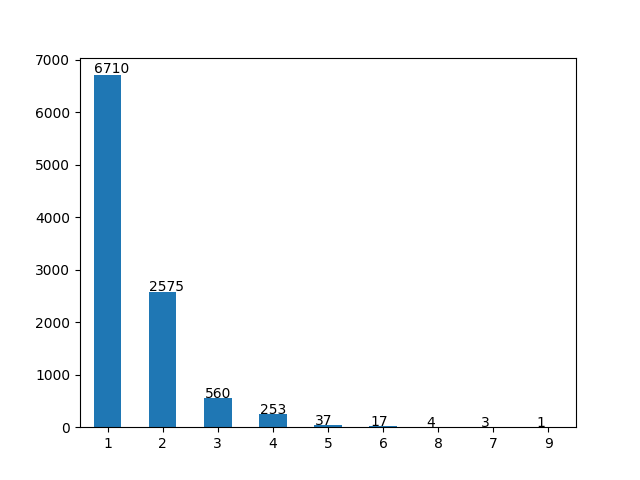
\includegraphics[scale=0.6]{data/analysis/labels_per_cases.png}
    \caption{Histogram representing the number of labels per cases for the multilabel dataset.}
\end{figure}



\section{Binary Classification}
\subsection{Best Results per Article}

This section presents the best results for several evaluation metrics and each article. It also reports the corresponding flavor.

	\begin{tabular}{|l|l|l|l| }
\hline
Article & Accuracy & Method & Flavor \\ \hline
Article 2 & 0.9708 (0.01) & Linear SVC & Descriptive and Bag-of-Words\\
Article 3 & 0.9532 (0.02) & Ensemble Extra Tree & Bag-of-Words only\\
Article 5 & 0.9627 (0.01) & Random Forest & Descriptive and Bag-of-Words\\
Article 6 & 0.9740 (0.01) & Ensemble Extra Tree & Descriptive and Bag-of-Words\\
Article 8 & 0.9568 (0.02) & Gradient Boosting & Descriptive and Bag-of-Words\\
Article 10 & 0.9509 (0.02) & Gradient Boosting & Descriptive and Bag-of-Words\\
Article 11 & 0.9672 (0.03) & Linear SVC & Descriptive and Bag-of-Words\\
Article 13 & 0.9704 (0.01) & Linear SVC & Descriptive and Bag-of-Words\\
Article 14 & 0.8854 (0.04) & Decision Tree & Descriptive and Bag-of-Words\\
Article 34 & 0.7567 (0.09) & Neural Net & Bag-of-Words only\\
Article p1-1 & 0.9745 (0.02) & Random Forest & Bag-of-Words only\\
Average & 0.9384 & & \\
Micro average & 0.9633 & & \\
\hline
\end{tabular}
	%\newpage
	\begin{tabular}{|l|l|l|l| }
\hline
Article & F1 score & Method & Flavor \\ \hline
Article 2 & 0.9702 & Linear SVC & Descriptive and Bag-of-Words\\
Article 3 & 0.9490 & Ensemble Extra Tree & Bag-of-Words only\\
Article 5 & 0.9607 & Random Forest & Descriptive and Bag-of-Words\\
Article 6 & 0.9735 & Ensemble Extra Tree & Descriptive and Bag-of-Words\\
Article 8 & 0.9565 & Gradient Boosting & Descriptive and Bag-of-Words\\
Article 10 & 0.9506 & Gradient Boosting & Descriptive and Bag-of-Words\\
Article 11 & 0.9680 & Ensemble Extra Tree & Descriptive and Bag-of-Words\\
Article 13 & 0.9678 & Linear SVC & Descriptive and Bag-of-Words\\
Article 14 & 0.8847 & Decision Tree & Descriptive and Bag-of-Words\\
Article 34 & 0.7216 & Neural Net & Bag-of-Words only\\
Article p1-1 & 0.9733 & Random Forest & Bag-of-Words only\\
Average & 0.9342 & & \\
Micro average & 0.9616 & & \\
\hline
\end{tabular}
	%\newpage
	\begin{tabular}{|l|l|l|l| }
\hline
Article & MCC & Method & Flavor \\ \hline
Article 2 & 0.8764 & Linear SVC & Descriptive and Bag-of-Words\\
Article 3 & 0.7454 & Ensemble Extra Tree & Bag-of-Words only\\
Article 5 & 0.7582 & Random Forest & Descriptive and Bag-of-Words\\
Article 6 & 0.8441 & Ensemble Extra Tree & Descriptive and Bag-of-Words\\
Article 8 & 0.8858 & Gradient Boosting & Descriptive and Bag-of-Words\\
Article 10 & 0.8595 & Gradient Boosting & Descriptive and Bag-of-Words\\
Article 11 & 0.8725 & Linear SVC & Descriptive and Bag-of-Words\\
Article 13 & 0.6940 & Linear SVC & Descriptive and Bag-of-Words\\
Article 14 & 0.7756 & Decision Tree & Descriptive and Bag-of-Words\\
Article 34 & 0.3795 & Neural Net & Bag-of-Words only\\
Article p1-1 & 0.8444 & Random Forest & Bag-of-Words only\\
Average & 0.7759 & & \\
Micro average & 0.8059 & & \\
\hline
\end{tabular}
	%\newpage
	\begin{tabular}{|l|l|l|l| }
\hline
Article & Precision & Method & Flavor \\ \hline
Article 2 & 0.9737 & Linear SVC & Descriptive and Bag-of-Words\\
Article 3 & 0.9515 & Ensemble Extra Tree & Bag-of-Words only\\
Article 5 & 0.9618 & Random Forest & Descriptive and Bag-of-Words\\
Article 6 & 0.9739 & Ensemble Extra Tree & Descriptive and Bag-of-Words\\
Article 8 & 0.9580 & Gradient Boosting & Descriptive and Bag-of-Words\\
Article 10 & 0.9522 & Gradient Boosting & Descriptive and Bag-of-Words\\
Article 11 & 0.9742 & Linear SVC & Descriptive and Bag-of-Words\\
Article 13 & 0.9694 & Linear SVC & Descriptive and Bag-of-Words\\
Article 14 & 0.8926 & Gradient Boosting & Descriptive and Bag-of-Words\\
Article 34 & 0.7395 & Neural Net & Bag-of-Words only\\
Article p1-1 & 0.9751 & Random Forest & Bag-of-Words only\\
Average & 0.9384 & & \\
Micro average & 0.9632 & & \\
\hline
\end{tabular}
	%\newpage
	\begin{tabular}{|l|l|l|l| }
\hline
Article & Recall & Method & Flavor \\ \hline
Article 2 & 0.9708 & Linear SVC & Descriptive and Bag-of-Words\\
Article 3 & 0.9532 & Ensemble Extra Tree & Bag-of-Words only\\
Article 5 & 0.9627 & Random Forest & Descriptive and Bag-of-Words\\
Article 6 & 0.9740 & Ensemble Extra Tree & Descriptive and Bag-of-Words\\
Article 8 & 0.9568 & Gradient Boosting & Descriptive and Bag-of-Words\\
Article 10 & 0.9509 & Gradient Boosting & Descriptive and Bag-of-Words\\
Article 11 & 0.9672 & Linear SVC & Descriptive and Bag-of-Words\\
Article 13 & 0.9704 & Linear SVC & Descriptive and Bag-of-Words\\
Article 14 & 0.8854 & Decision Tree & Descriptive and Bag-of-Words\\
Article 34 & 0.7567 & Neural Net & Bag-of-Words only\\
Article p1-1 & 0.9745 & Random Forest & Bag-of-Words only\\
Average & 0.9384 & & \\
Micro average & 0.9633 & & \\
\hline
\end{tabular}
	%\newpage

\subsection{Summary \& Method ranking}

	\begin{tabular}{|l|l|l|l| }
\hline
Method                  & Accuracy & Micro Accuracy & Rank \\ \hline
Linear SVC              & 0.9350 & 0.9610 & 1\\
Ensemble Extra Tree     & 0.9315 & 0.9615 & 2\\
Gradient Boosting       & 0.9297 & 0.9602 & 3\\
Random Forest           & 0.9274 & 0.9608 & 4\\
BaggingClassifier       & 0.9238 & 0.9588 & 5\\
Neural Net              & 0.9194 & 0.9498 & 6\\
AdaBoost                & 0.9187 & 0.9494 & 7\\
Decision Tree           & 0.9162 & 0.9451 & 8\\
Extra Tree              & 0.8821 & 0.9226 & 9\\
Bernoulli Naive Bayes   & 0.8648 & 0.9006 & 10\\
Multinomial Naive Bayes & 0.8589 & 0.8995 & 11\\
K-Neighbors             & 0.8523 & 0.8947 & 12\\
Average & 0.9050 & 0.9386 & \\
\hline
\end{tabular}\\
	\newpage
	\begin{tabular}{|l|l|l| }
\hline
Method                  & F1 score & Rank \\ \hline
Linear SVC              & 0.9308 & 1\\
Gradient Boosting       & 0.9272 & 2\\
Ensemble Extra Tree     & 0.9236 & 3\\
BaggingClassifier       & 0.9213 & 4\\
Random Forest           & 0.9176 & 5\\
Decision Tree           & 0.9162 & 6\\
AdaBoost                & 0.9158 & 7\\
Neural Net              & 0.9125 & 8\\
Extra Tree              & 0.8807 & 9\\
Bernoulli Naive Bayes   & 0.8298 & 10\\
Multinomial Naive Bayes & 0.8219 & 11\\
K-Neighbors             & 0.8193 & 12\\
Average & 0.8931 & \\
\hline
\end{tabular}\\
	\newpage
	\begin{tabular}{|l|l|l| }
\hline
Method                  & MCC & Rank \\ \hline
Linear SVC              & 0.7662 & 1\\
Ensemble Extra Tree     & 0.7544 & 2\\
Gradient Boosting       & 0.7473 & 3\\
Random Forest           & 0.7366 & 4\\
BaggingClassifier       & 0.7343 & 5\\
Decision Tree           & 0.7027 & 6\\
AdaBoost                & 0.6939 & 7\\
Neural Net              & 0.6799 & 8\\
Extra Tree              & 0.5718 & 9\\
Bernoulli Naive Bayes   & 0.3327 & 10\\
Multinomial Naive Bayes & 0.3084 & 11\\
K-Neighbors             & 0.2952 & 12\\
Average & 0.6103 & \\
\hline
\end{tabular}\\
	\newpage
	\begin{tabular}{|l|l|l| }
\hline
Method                  & Precision & Rank \\ \hline
Linear SVC              & 0.9344 & 1\\
Ensemble Extra Tree     & 0.9313 & 2\\
Gradient Boosting       & 0.9301 & 3\\
BaggingClassifier       & 0.9247 & 4\\
Neural Net              & 0.9229 & 5\\
Random Forest           & 0.9220 & 6\\
Decision Tree           & 0.9211 & 7\\
AdaBoost                & 0.9191 & 8\\
Extra Tree              & 0.8842 & 9\\
K-Neighbors             & 0.8189 & 10\\
Bernoulli Naive Bayes   & 0.8181 & 11\\
Multinomial Naive Bayes & 0.8079 & 12\\
Average & 0.8945 & \\
\hline
\end{tabular}\\
	\newpage
	\begin{tabular}{|l|l|l| }
\hline
Method                  & Recall & Rank \\ \hline
Linear SVC              & 0.9350 & 1\\
Ensemble Extra Tree     & 0.9315 & 2\\
Gradient Boosting       & 0.9297 & 3\\
Random Forest           & 0.9274 & 4\\
BaggingClassifier       & 0.9238 & 5\\
Neural Net              & 0.9194 & 6\\
AdaBoost                & 0.9187 & 7\\
Decision Tree           & 0.9162 & 8\\
Extra Tree              & 0.8821 & 9\\
Bernoulli Naive Bayes   & 0.8648 & 10\\
Multinomial Naive Bayes & 0.8589 & 11\\
K-Neighbors             & 0.8523 & 12\\
Average & 0.9050 & \\
\hline
\end{tabular}\\
	\newpage

\subsection{Detailed Results}

This section presents the results for each method on each article and for all evaluation metrics.
It also reports the best normalized confusion matrices for each article.\\

\noindent
	\begin{tabular}{|l|l|l|l| }
\hline
Prev=0.7773 &  \multicolumn{3}{c|}{Accuracy - Article 10} \\
\cline{2-4} & desc & BoW & both \\ \hline
AdaBoost                & 0.8359 (0.06) & 0.9313 (0.03) & 0.9187 (0.02)\\
BaggingClassifier       & {\bf 0.8767} (0.04) & 0.9342 (0.03) & 0.9495 (0.02)\\
Bernoulli Naive Bayes   & 0.7773 (0.00) & 0.7801 (0.02) & 0.7745 (0.01)\\
Decision Tree           & 0.8445 (0.03) & 0.9076 (0.04) & 0.9243 (0.03)\\
Ensemble Extra Tree     & 0.8025 (0.03) & 0.9468 (0.03) & 0.9482 (0.03)\\
Extra Tree              & 0.7564 (0.08) & 0.8599 (0.06) & 0.8727 (0.05)\\
Gradient Boosting       & 0.8697 (0.06) & 0.9371 (0.03) & {\bf 0.9509} (0.02)\\
K-Neighbors             & 0.8291 (0.05) & 0.7773 (0.00) & 0.7773 (0.00)\\
Linear SVC              & 0.8529 (0.05) & {\bf 0.9496} (0.02) & 0.9495 (0.02)\\
Multinomial Naive Bayes & 0.7773 (0.00) & 0.7787 (0.01) & 0.7773 (0.00)\\
Neural Net              & 0.8178 (0.09) & 0.9285 (0.03) & 0.9312 (0.04)\\
Random Forest           & 0.7856 (0.02) & 0.9468 (0.03) & 0.9482 (0.03)\\
\hline
\end{tabular}~\\
	%\newpage
	\begin{tabular}{|l|l|l|l| }
\hline
Prev=0.8618 &  \multicolumn{3}{c|}{Accuracy - Article 11} \\
\cline{2-4} & desc & BoW & both \\ \hline
AdaBoost                & 0.8877 (0.04) & 0.9202 (0.04) & 0.9378 (0.05)\\
BaggingClassifier       & 0.9164 (0.04) & 0.9270 (0.05) & 0.9525 (0.04)\\
Bernoulli Naive Bayes   & 0.8619 (0.01) & 0.8583 (0.02) & 0.8619 (0.01)\\
Decision Tree           & 0.8733 (0.06) & 0.9235 (0.05) & 0.9414 (0.05)\\
Ensemble Extra Tree     & 0.8582 (0.02) & 0.9562 (0.03) & 0.9669 (0.04)\\
Extra Tree              & 0.8619 (0.04) & 0.8940 (0.05) & 0.8948 (0.06)\\
Gradient Boosting       & 0.8870 (0.04) & 0.9304 (0.06) & 0.9525 (0.04)\\
K-Neighbors             & 0.8692 (0.04) & 0.8619 (0.01) & 0.8619 (0.01)\\
Linear SVC              & {\bf 0.9238} (0.06) & {\bf 0.9636} (0.03) & {\bf 0.9672} (0.03)\\
Multinomial Naive Bayes & 0.8619 (0.01) & 0.8583 (0.02) & 0.8619 (0.01)\\
Neural Net              & 0.8730 (0.07) & 0.9090 (0.06) & 0.9197 (0.05)\\
Random Forest           & 0.8582 (0.02) & 0.9561 (0.04) & 0.9198 (0.03)\\
\hline
\end{tabular}~\\
	%\newpage
	\begin{tabular}{|l|l|l|l| }
\hline
Prev=0.9434 &  \multicolumn{3}{c|}{Accuracy - Article 13} \\
\cline{2-4} & desc & BoW & both \\ \hline
AdaBoost                & 0.9455 (0.01) & 0.9501 (0.01) & 0.9506 (0.01)\\
BaggingClassifier       & 0.9486 (0.01) & 0.9642 (0.01) & 0.9683 (0.01)\\
Bernoulli Naive Bayes   & 0.9429 (0.00) & 0.9252 (0.03) & 0.9356 (0.01)\\
Decision Tree           & 0.9403 (0.01) & 0.9413 (0.02) & 0.9595 (0.01)\\
Ensemble Extra Tree     & 0.9475 (0.01) & 0.9688 (0.01) & 0.9699 (0.01)\\
Extra Tree              & 0.9309 (0.03) & 0.9356 (0.02) & 0.9314 (0.01)\\
Gradient Boosting       & 0.9507 (0.00) & 0.9657 (0.01) & 0.9657 (0.01)\\
K-Neighbors             & 0.9465 (0.00) & 0.9434 (0.00) & 0.9434 (0.00)\\
Linear SVC              & {\bf 0.9590} (0.01) & {\bf 0.9693} (0.01) & {\bf 0.9704} (0.01)\\
Multinomial Naive Bayes & 0.9382 (0.01) & 0.9361 (0.02) & 0.9403 (0.01)\\
Neural Net              & 0.9522 (0.02) & 0.9512 (0.01) & 0.9532 (0.01)\\
Random Forest           & 0.9475 (0.00) & 0.9688 (0.01) & 0.9647 (0.01)\\
\hline
\end{tabular}~\\
	%\newpage
	\begin{tabular}{|l|l|l|l| }
\hline
Prev=0.5461 &  \multicolumn{3}{c|}{Accuracy - Article 14} \\
\cline{2-4} & desc & BoW & both \\ \hline
AdaBoost                & 0.8352 (0.06) & 0.8329 (0.07) & 0.8702 (0.06)\\
BaggingClassifier       & 0.8428 (0.04) & 0.8604 (0.08) & 0.8653 (0.08)\\
Bernoulli Naive Bayes   & 0.5462 (0.01) & 0.8280 (0.10) & 0.7433 (0.08)\\
Decision Tree           & 0.8102 (0.10) & 0.7956 (0.05) & {\bf 0.8854} (0.04)\\
Ensemble Extra Tree     & 0.8107 (0.09) & 0.8752 (0.08) & 0.8678 (0.07)\\
Extra Tree              & 0.7111 (0.10) & 0.7354 (0.08) & 0.7657 (0.06)\\
Gradient Boosting       & {\bf 0.8727} (0.06) & 0.8802 (0.06) & 0.8852 (0.06)\\
K-Neighbors             & 0.6683 (0.07) & 0.7035 (0.11) & 0.6984 (0.09)\\
Linear SVC              & 0.8704 (0.06) & {\bf 0.8803} (0.06) & 0.8828 (0.07)\\
Multinomial Naive Bayes & 0.7683 (0.09) & 0.7982 (0.12) & 0.7706 (0.09)\\
Neural Net              & 0.8404 (0.06) & 0.8578 (0.08) & 0.8652 (0.10)\\
Random Forest           & 0.7979 (0.10) & 0.8602 (0.07) & 0.8677 (0.07)\\
\hline
\end{tabular}~\\
	%\newpage
	\begin{tabular}{|l|l|l|l| }
\hline
Prev=0.8697 &  \multicolumn{3}{c|}{Accuracy - Article 2} \\
\cline{2-4} & desc & BoW & both \\ \hline
AdaBoost                & 0.8888 (0.03) & 0.9561 (0.02) & 0.9488 (0.02)\\
BaggingClassifier       & 0.8888 (0.05) & 0.9620 (0.02) & 0.9620 (0.02)\\
Bernoulli Naive Bayes   & 0.8697 (0.00) & 0.8741 (0.03) & 0.8668 (0.01)\\
Decision Tree           & 0.8843 (0.04) & 0.9458 (0.03) & 0.9474 (0.02)\\
Ensemble Extra Tree     & 0.8932 (0.03) & 0.9678 (0.02) & 0.9693 (0.02)\\
Extra Tree              & 0.8639 (0.04) & 0.9110 (0.05) & 0.9210 (0.05)\\
Gradient Boosting       & 0.8962 (0.03) & 0.9635 (0.02) & 0.9620 (0.02)\\
K-Neighbors             & 0.8903 (0.03) & 0.8990 (0.03) & 0.8990 (0.03)\\
Linear SVC              & {\bf 0.9180} (0.03) & {\bf 0.9693} (0.02) & {\bf 0.9708} (0.01)\\
Multinomial Naive Bayes & 0.8741 (0.01) & 0.8727 (0.02) & 0.8682 (0.01)\\
Neural Net              & 0.8990 (0.03) & 0.9430 (0.03) & 0.9459 (0.03)\\
Random Forest           & 0.8917 (0.03) & {\bf 0.9693} (0.02) & 0.9649 (0.02)\\
\hline
\end{tabular}~\\
	%\newpage
	\begin{tabular}{|l|l|l|l| }
\hline
Prev=0.8856 &  \multicolumn{3}{c|}{Accuracy - Article 3} \\
\cline{2-4} & desc & BoW & both \\ \hline
AdaBoost                & 0.9054 (0.01) & 0.9346 (0.02) & 0.9342 (0.02)\\
BaggingClassifier       & 0.9121 (0.02) & 0.9426 (0.03) & 0.9483 (0.02)\\
Bernoulli Naive Bayes   & 0.8856 (0.00) & 0.9006 (0.03) & 0.8895 (0.01)\\
Decision Tree           & 0.8957 (0.01) & 0.9147 (0.03) & 0.9346 (0.02)\\
Ensemble Extra Tree     & 0.9090 (0.01) & {\bf 0.9532} (0.02) & {\bf 0.9528} (0.02)\\
Extra Tree              & 0.8723 (0.02) & 0.9152 (0.02) & 0.9019 (0.02)\\
Gradient Boosting       & 0.9143 (0.01) & 0.9479 (0.02) & 0.9492 (0.03)\\
K-Neighbors             & 0.9055 (0.03) & 0.8860 (0.00) & 0.8856 (0.00)\\
Linear SVC              & {\bf 0.9209} (0.02) & 0.9501 (0.03) & 0.9523 (0.03)\\
Multinomial Naive Bayes & 0.8878 (0.01) & 0.9072 (0.02) & 0.8953 (0.01)\\
Neural Net              & 0.9152 (0.01) & 0.9390 (0.02) & 0.9373 (0.02)\\
Random Forest           & 0.9037 (0.02) & 0.9523 (0.03) & 0.9514 (0.03)\\
\hline
\end{tabular}~\\
	%\newpage
	\begin{tabular}{|l|l|l|l| }
\hline
Prev=0.674 &  \multicolumn{3}{c|}{Accuracy - Article 34} \\
\cline{2-4} & desc & BoW & both \\ \hline
AdaBoost                & 0.6687 (0.10) & 0.7126 (0.05) & 0.6629 (0.09)\\
BaggingClassifier       & 0.6070 (0.09) & 0.6465 (0.09) & 0.6635 (0.09)\\
Bernoulli Naive Bayes   & 0.6740 (0.02) & 0.6740 (0.02) & 0.6740 (0.02)\\
Decision Tree           & 0.6073 (0.11) & 0.6901 (0.08) & 0.6360 (0.09)\\
Ensemble Extra Tree     & 0.6626 (0.04) & 0.7012 (0.05) & 0.7073 (0.03)\\
Extra Tree              & 0.6184 (0.06) & 0.5915 (0.10) & 0.6857 (0.08)\\
Gradient Boosting       & 0.6237 (0.08) & 0.7015 (0.05) & 0.6959 (0.05)\\
K-Neighbors             & 0.6681 (0.03) & 0.6740 (0.02) & 0.6740 (0.02)\\
Linear SVC              & 0.6792 (0.09) & 0.7345 (0.08) & {\bf 0.7401} (0.08)\\
Multinomial Naive Bayes & 0.6740 (0.02) & 0.6740 (0.02) & 0.6740 (0.02)\\
Neural Net              & {\bf 0.6845} (0.08) & {\bf 0.7567} (0.09) & 0.7123 (0.12)\\
Random Forest           & 0.6573 (0.02) & 0.6792 (0.06) & 0.6795 (0.03)\\
\hline
\end{tabular}~\\
	%\newpage
	\begin{tabular}{|l|l|l|l| }
\hline
Prev=0.9096 &  \multicolumn{3}{c|}{Accuracy - Article 5} \\
\cline{2-4} & desc & BoW & both \\ \hline
AdaBoost                & 0.9177 (0.02) & 0.9435 (0.02) & 0.9464 (0.02)\\
BaggingClassifier       & 0.9124 (0.02) & 0.9531 (0.01) & 0.9560 (0.01)\\
Bernoulli Naive Bayes   & 0.9091 (0.00) & 0.9038 (0.03) & 0.9038 (0.01)\\
Decision Tree           & 0.9057 (0.03) & 0.9316 (0.02) & 0.9445 (0.02)\\
Ensemble Extra Tree     & 0.9096 (0.02) & {\bf 0.9608} (0.01) & 0.9622 (0.01)\\
Extra Tree              & 0.8861 (0.02) & 0.9258 (0.02) & 0.9220 (0.03)\\
Gradient Boosting       & 0.9144 (0.02) & 0.9579 (0.01) & 0.9574 (0.01)\\
K-Neighbors             & 0.9158 (0.01) & 0.9105 (0.00) & 0.9105 (0.00)\\
Linear SVC              & {\bf 0.9273} (0.01) & 0.9603 (0.01) & 0.9622 (0.01)\\
Multinomial Naive Bayes & 0.9091 (0.00) & 0.9096 (0.02) & 0.9072 (0.01)\\
Neural Net              & 0.9239 (0.02) & 0.9431 (0.01) & 0.9450 (0.01)\\
Random Forest           & 0.9096 (0.00) & 0.9598 (0.01) & {\bf 0.9627} (0.01)\\
\hline
\end{tabular}~\\
	%\newpage
	\begin{tabular}{|l|l|l|l| }
\hline
Prev=0.9061 &  \multicolumn{3}{c|}{Accuracy - Article 6} \\
\cline{2-4} & desc & BoW & both \\ \hline
AdaBoost                & 0.9301 (0.02) & 0.9624 (0.01) & 0.9670 (0.01)\\
BaggingClassifier       & {\bf 0.9411} (0.02) & 0.9690 (0.01) & 0.9731 (0.01)\\
Bernoulli Naive Bayes   & 0.9001 (0.01) & 0.8902 (0.04) & 0.9056 (0.04)\\
Decision Tree           & 0.9239 (0.02) & 0.9528 (0.01) & 0.9560 (0.02)\\
Ensemble Extra Tree     & 0.9222 (0.01) & 0.9733 (0.01) & {\bf 0.9740} (0.01)\\
Extra Tree              & 0.8903 (0.02) & 0.9367 (0.01) & 0.9420 (0.02)\\
Gradient Boosting       & 0.9392 (0.02) & 0.9714 (0.01) & 0.9735 (0.01)\\
K-Neighbors             & 0.9079 (0.01) & 0.9068 (0.00) & 0.9071 (0.00)\\
Linear SVC              & 0.9409 (0.01) & 0.9700 (0.01) & 0.9718 (0.01)\\
Multinomial Naive Bayes & 0.9068 (0.00) & 0.8955 (0.04) & 0.9121 (0.04)\\
Neural Net              & 0.9322 (0.01) & 0.9694 (0.01) & 0.9695 (0.02)\\
Random Forest           & 0.9174 (0.01) & {\bf 0.9737} (0.01) & 0.9730 (0.01)\\
\hline
\end{tabular}~\\
	%\newpage
	\begin{tabular}{|l|l|l|l| }
\hline
Prev=0.7497 &  \multicolumn{3}{c|}{Accuracy - Article 8} \\
\cline{2-4} & desc & BoW & both \\ \hline
AdaBoost                & 0.8710 (0.04) & 0.9323 (0.03) & 0.9274 (0.02)\\
BaggingClassifier       & 0.8724 (0.04) & 0.9442 (0.02) & 0.9561 (0.01)\\
Bernoulli Naive Bayes   & 0.7497 (0.00) & 0.9260 (0.06) & 0.8013 (0.02)\\
Decision Tree           & 0.8515 (0.04) & 0.9135 (0.03) & 0.9386 (0.01)\\
Ensemble Extra Tree     & 0.8152 (0.02) & {\bf 0.9477} (0.03) & 0.9477 (0.03)\\
Extra Tree              & 0.7678 (0.05) & 0.8772 (0.05) & 0.8968 (0.03)\\
Gradient Boosting       & {\bf 0.8835} (0.04) & 0.9449 (0.02) & {\bf 0.9568} (0.02)\\
K-Neighbors             & 0.8054 (0.02) & 0.7538 (0.01) & 0.7538 (0.01)\\
Linear SVC              & 0.8696 (0.03) & 0.9449 (0.03) & 0.9456 (0.03)\\
Multinomial Naive Bayes & 0.7594 (0.01) & 0.8807 (0.03) & 0.7734 (0.03)\\
Neural Net              & 0.8214 (0.03) & 0.9386 (0.04) & 0.9372 (0.05)\\
Random Forest           & 0.8131 (0.02) & 0.9456 (0.03) & 0.9484 (0.03)\\
\hline
\end{tabular}~\\
	%\newpage
	\begin{tabular}{|l|l|l|l| }
\hline
Prev=0.9064 &  \multicolumn{3}{c|}{Accuracy - Article p1-1} \\
\cline{2-4} & desc & BoW & both \\ \hline
AdaBoost                & 0.9178 (0.02) & 0.9667 (0.02) & 0.9653 (0.02)\\
BaggingClassifier       & 0.9334 (0.02) & 0.9660 (0.02) & 0.9674 (0.02)\\
Bernoulli Naive Bayes   & 0.9057 (0.00) & 0.9107 (0.03) & 0.9050 (0.02)\\
Decision Tree           & 0.9327 (0.02) & 0.9561 (0.03) & 0.9561 (0.02)\\
Ensemble Extra Tree     & 0.9093 (0.02) & 0.9724 (0.02) & 0.9731 (0.02)\\
Extra Tree              & 0.8902 (0.02) & 0.9327 (0.03) & 0.9483 (0.04)\\
Gradient Boosting       & {\bf 0.9433} (0.02) & 0.9695 (0.02) & 0.9695 (0.02)\\
K-Neighbors             & 0.9065 (0.01) & 0.9150 (0.01) & 0.9192 (0.01)\\
Linear SVC              & 0.9298 (0.02) & 0.9724 (0.01) & 0.9724 (0.01)\\
Multinomial Naive Bayes & 0.9057 (0.00) & 0.9114 (0.03) & 0.9079 (0.01)\\
Neural Net              & 0.9164 (0.01) & 0.9490 (0.02) & 0.9476 (0.02)\\
Random Forest           & 0.9100 (0.01) & {\bf 0.9745} (0.02) & {\bf 0.9745} (0.01)\\
\hline
\end{tabular}~\\
	%\newpage
	\begin{tabular}{|l|l|l|l| }
\hline
Prev=0.7773 &  \multicolumn{3}{c|}{F1 score - Article 10} \\
\cline{2-4} & desc & BoW & both \\ \hline
AdaBoost                & 0.8296 & 0.9311 & 0.9186\\
BaggingClassifier       & {\bf 0.8749} & 0.9338 & 0.9493\\
Bernoulli Naive Bayes   & 0.6799 & 0.6965 & 0.6785\\
Decision Tree           & 0.8444 & 0.9079 & 0.9245\\
Ensemble Extra Tree     & 0.7522 & 0.9471 & 0.9485\\
Extra Tree              & 0.7436 & 0.8583 & 0.8713\\
Gradient Boosting       & 0.8616 & 0.9377 & {\bf 0.9506}\\
K-Neighbors             & 0.8158 & 0.6799 & 0.6799\\
Linear SVC              & 0.8408 & {\bf 0.9496} & 0.9495\\
Multinomial Naive Bayes & 0.6799 & 0.6874 & 0.6799\\
Neural Net              & 0.8043 & 0.9262 & 0.9296\\
Random Forest           & 0.7169 & 0.9471 & 0.9483\\
\hline
\end{tabular}~\\
	%\newpage
	\begin{tabular}{|l|l|l|l| }
\hline
Prev=0.8618 &  \multicolumn{3}{c|}{F1 score - Article 11} \\
\cline{2-4} & desc & BoW & both \\ \hline
AdaBoost                & 0.8822 & 0.9059 & 0.9353\\
BaggingClassifier       & 0.9041 & 0.9328 & 0.9554\\
Bernoulli Naive Bayes   & 0.7980 & 0.7962 & 0.7980\\
Decision Tree           & 0.8682 & 0.9212 & 0.9428\\
Ensemble Extra Tree     & 0.7962 & 0.9579 & {\bf 0.9680}\\
Extra Tree              & 0.8501 & 0.8976 & 0.8918\\
Gradient Boosting       & 0.8693 & 0.9349 & 0.9545\\
K-Neighbors             & 0.8363 & 0.7980 & 0.7980\\
Linear SVC              & {\bf 0.9063} & {\bf 0.9634} & 0.9671\\
Multinomial Naive Bayes & 0.7980 & 0.7962 & 0.7980\\
Neural Net              & 0.8446 & 0.8969 & 0.9216\\
Random Forest           & 0.7962 & 0.9569 & 0.9115\\
\hline
\end{tabular}~\\
	%\newpage
	\begin{tabular}{|l|l|l|l| }
\hline
Prev=0.9434 &  \multicolumn{3}{c|}{F1 score - Article 13} \\
\cline{2-4} & desc & BoW & both \\ \hline
AdaBoost                & 0.9393 & 0.9470 & 0.9478\\
BaggingClassifier       & 0.9408 & 0.9604 & 0.9649\\
Bernoulli Naive Bayes   & 0.9156 & 0.9224 & 0.9141\\
Decision Tree           & 0.9352 & 0.9423 & 0.9585\\
Ensemble Extra Tree     & 0.9266 & 0.9636 & 0.9655\\
Extra Tree              & 0.9281 & 0.9357 & 0.9276\\
Gradient Boosting       & 0.9378 & 0.9624 & 0.9619\\
K-Neighbors             & 0.9235 & 0.9159 & 0.9159\\
Linear SVC              & {\bf 0.9547} & {\bf 0.9659} & {\bf 0.9678}\\
Multinomial Naive Bayes & 0.9133 & 0.9293 & 0.9176\\
Neural Net              & 0.9455 & 0.9354 & 0.9388\\
Random Forest           & 0.9250 & 0.9641 & 0.9567\\
\hline
\end{tabular}~\\
	%\newpage
	\begin{tabular}{|l|l|l|l| }
\hline
Prev=0.5461 &  \multicolumn{3}{c|}{F1 score - Article 14} \\
\cline{2-4} & desc & BoW & both \\ \hline
AdaBoost                & 0.8335 & 0.8322 & 0.8700\\
BaggingClassifier       & 0.8407 & 0.8594 & 0.8646\\
Bernoulli Naive Bayes   & 0.3859 & 0.8225 & 0.7152\\
Decision Tree           & 0.8069 & 0.7935 & {\bf 0.8847}\\
Ensemble Extra Tree     & 0.8057 & 0.8734 & 0.8655\\
Extra Tree              & 0.7076 & 0.7311 & 0.7632\\
Gradient Boosting       & {\bf 0.8700} & 0.8795 & 0.8839\\
K-Neighbors             & 0.6173 & 0.6994 & 0.6936\\
Linear SVC              & 0.8690 & {\bf 0.8797} & 0.8823\\
Multinomial Naive Bayes & 0.7540 & 0.7899 & 0.7551\\
Neural Net              & 0.8390 & 0.8557 & 0.8608\\
Random Forest           & 0.7863 & 0.8579 & 0.8663\\
\hline
\end{tabular}~\\
	%\newpage
	\begin{tabular}{|l|l|l|l| }
\hline
Prev=0.8697 &  \multicolumn{3}{c|}{F1 score - Article 2} \\
\cline{2-4} & desc & BoW & both \\ \hline
AdaBoost                & 0.8837 & 0.9556 & 0.9480\\
BaggingClassifier       & 0.8742 & 0.9614 & 0.9608\\
Bernoulli Naive Bayes   & 0.8091 & 0.8240 & 0.8102\\
Decision Tree           & 0.8804 & 0.9455 & 0.9476\\
Ensemble Extra Tree     & 0.8620 & 0.9675 & 0.9687\\
Extra Tree              & 0.8493 & 0.9128 & 0.9205\\
Gradient Boosting       & 0.8701 & 0.9633 & 0.9615\\
K-Neighbors             & 0.8556 & 0.8643 & 0.8644\\
Linear SVC              & {\bf 0.9083} & 0.9688 & {\bf 0.9702}\\
Multinomial Naive Bayes & 0.8184 & 0.8230 & 0.8109\\
Neural Net              & 0.8859 & 0.9340 & 0.9390\\
Random Forest           & 0.8572 & {\bf 0.9691} & 0.9642\\
\hline
\end{tabular}~\\
	%\newpage
	\begin{tabular}{|l|l|l|l| }
\hline
Prev=0.8856 &  \multicolumn{3}{c|}{F1 score - Article 3} \\
\cline{2-4} & desc & BoW & both \\ \hline
AdaBoost                & 0.8931 & 0.9311 & 0.9296\\
BaggingClassifier       & 0.8992 & 0.9391 & 0.9442\\
Bernoulli Naive Bayes   & 0.8318 & 0.8989 & 0.8618\\
Decision Tree           & 0.8896 & 0.9153 & 0.9325\\
Ensemble Extra Tree     & 0.8840 & {\bf 0.9490} & {\bf 0.9486}\\
Extra Tree              & 0.8640 & 0.9141 & 0.9010\\
Gradient Boosting       & 0.8938 & 0.9450 & 0.9451\\
K-Neighbors             & 0.8832 & 0.8328 & 0.8318\\
Linear SVC              & {\bf 0.9094} & 0.9462 & 0.9482\\
Multinomial Naive Bayes & 0.8391 & 0.8989 & 0.8611\\
Neural Net              & 0.9070 & 0.9311 & 0.9285\\
Random Forest           & 0.8747 & 0.9480 & 0.9472\\
\hline
\end{tabular}~\\
	%\newpage
	\begin{tabular}{|l|l|l|l| }
\hline
Prev=0.674 &  \multicolumn{3}{c|}{F1 score - Article 34} \\
\cline{2-4} & desc & BoW & both \\ \hline
AdaBoost                & {\bf 0.6621} & 0.6953 & 0.6337\\
BaggingClassifier       & 0.5719 & 0.6305 & 0.6465\\
Bernoulli Naive Bayes   & 0.5428 & 0.5428 & 0.5428\\
Decision Tree           & 0.5950 & 0.6903 & 0.6379\\
Ensemble Extra Tree     & 0.5447 & 0.6331 & 0.6322\\
Extra Tree              & 0.5706 & 0.5866 & 0.6764\\
Gradient Boosting       & 0.5770 & 0.6841 & 0.6774\\
K-Neighbors             & 0.5479 & 0.5428 & 0.5428\\
Linear SVC              & 0.6338 & 0.6993 & {\bf 0.7044}\\
Multinomial Naive Bayes & 0.5428 & 0.5428 & 0.5428\\
Neural Net              & 0.6408 & {\bf 0.7216} & 0.6999\\
Random Forest           & 0.5343 & 0.5856 & 0.5761\\
\hline
\end{tabular}~\\
	%\newpage
	\begin{tabular}{|l|l|l|l| }
\hline
Prev=0.9096 &  \multicolumn{3}{c|}{F1 score - Article 5} \\
\cline{2-4} & desc & BoW & both \\ \hline
AdaBoost                & 0.9086 & 0.9404 & 0.9428\\
BaggingClassifier       & 0.9040 & 0.9514 & 0.9547\\
Bernoulli Naive Bayes   & 0.8663 & 0.8869 & 0.8674\\
Decision Tree           & 0.8994 & 0.9320 & 0.9446\\
Ensemble Extra Tree     & 0.8818 & {\bf 0.9590} & 0.9606\\
Extra Tree              & 0.8773 & 0.9231 & 0.9224\\
Gradient Boosting       & 0.8992 & 0.9568 & 0.9566\\
K-Neighbors             & 0.8957 & 0.8687 & 0.8687\\
Linear SVC              & 0.9150 & 0.9582 & 0.9602\\
Multinomial Naive Bayes & 0.8663 & 0.8865 & 0.8677\\
Neural Net              & {\bf 0.9160} & 0.9349 & 0.9374\\
Random Forest           & 0.8744 & 0.9582 & {\bf 0.9607}\\
\hline
\end{tabular}~\\
	%\newpage
	\begin{tabular}{|l|l|l|l| }
\hline
Prev=0.9061 &  \multicolumn{3}{c|}{F1 score - Article 6} \\
\cline{2-4} & desc & BoW & both \\ \hline
AdaBoost                & 0.9249 & 0.9620 & 0.9661\\
BaggingClassifier       & {\bf 0.9375} & 0.9684 & 0.9722\\
Bernoulli Naive Bayes   & 0.8632 & 0.9039 & 0.9115\\
Decision Tree           & 0.9224 & 0.9522 & 0.9564\\
Ensemble Extra Tree     & 0.9015 & 0.9727 & {\bf 0.9735}\\
Extra Tree              & 0.8838 & 0.9373 & 0.9414\\
Gradient Boosting       & 0.9321 & 0.9711 & 0.9730\\
K-Neighbors             & 0.8752 & 0.8634 & 0.8641\\
Linear SVC              & 0.9348 & 0.9696 & 0.9714\\
Multinomial Naive Bayes & 0.8775 & 0.9072 & 0.9167\\
Neural Net              & 0.9248 & 0.9690 & 0.9691\\
Random Forest           & 0.8915 & {\bf 0.9732} & 0.9725\\
\hline
\end{tabular}~\\
	%\newpage
	\begin{tabular}{|l|l|l|l| }
\hline
Prev=0.7497 &  \multicolumn{3}{c|}{F1 score - Article 8} \\
\cline{2-4} & desc & BoW & both \\ \hline
AdaBoost                & 0.8667 & 0.9325 & 0.9276\\
BaggingClassifier       & 0.8702 & 0.9443 & 0.9553\\
Bernoulli Naive Bayes   & 0.6424 & 0.9277 & 0.7522\\
Decision Tree           & 0.8478 & 0.9136 & 0.9389\\
Ensemble Extra Tree     & 0.7855 & {\bf 0.9479} & 0.9479\\
Extra Tree              & 0.7529 & 0.8758 & 0.8961\\
Gradient Boosting       & {\bf 0.8785} & 0.9450 & {\bf 0.9565}\\
K-Neighbors             & 0.7827 & 0.6516 & 0.6516\\
Linear SVC              & 0.8663 & 0.9453 & 0.9460\\
Multinomial Naive Bayes & 0.6660 & 0.8748 & 0.6932\\
Neural Net              & 0.8144 & 0.9391 & 0.9381\\
Random Forest           & 0.7773 & 0.9458 & 0.9485\\
\hline
\end{tabular}~\\
	%\newpage
	\begin{tabular}{|l|l|l|l| }
\hline
Prev=0.9064 &  \multicolumn{3}{c|}{F1 score - Article p1-1} \\
\cline{2-4} & desc & BoW & both \\ \hline
AdaBoost                & 0.9070 & 0.9656 & 0.9645\\
BaggingClassifier       & 0.9222 & 0.9649 & 0.9663\\
Bernoulli Naive Bayes   & 0.8616 & 0.8961 & 0.8684\\
Decision Tree           & 0.9276 & 0.9568 & 0.9568\\
Ensemble Extra Tree     & 0.8769 & 0.9709 & 0.9717\\
Extra Tree              & 0.8804 & 0.9320 & 0.9487\\
Gradient Boosting       & {\bf 0.9327} & 0.9685 & 0.9684\\
K-Neighbors             & 0.8681 & 0.8816 & 0.8887\\
Linear SVC              & 0.9178 & 0.9713 & 0.9713\\
Multinomial Naive Bayes & 0.8616 & 0.8930 & 0.8711\\
Neural Net              & 0.9010 & 0.9429 & 0.9423\\
Random Forest           & 0.8720 & {\bf 0.9733} & {\bf 0.9731}\\
\hline
\end{tabular}~\\
	%\newpage
	\begin{tabular}{|l|l|l|l| }
\hline
Prev=0.7773 &  \multicolumn{3}{c|}{MCC - Article 10} \\
\cline{2-4} & desc & BoW & both \\ \hline
AdaBoost                & 0.5094 & 0.8094 & 0.7716\\
BaggingClassifier       & {\bf 0.6441} & 0.8121 & 0.8551\\
Bernoulli Naive Bayes   & 0.0000 & 0.0741 & -0.0129\\
Decision Tree           & 0.5610 & 0.7434 & 0.7900\\
Ensemble Extra Tree     & 0.2990 & 0.8520 & 0.8564\\
Extra Tree              & 0.2588 & 0.5935 & 0.6307\\
Gradient Boosting       & 0.5949 & 0.8271 & {\bf 0.8595}\\
K-Neighbors             & 0.4667 & 0.0000 & 0.0000\\
Linear SVC              & 0.5419 & {\bf 0.8569} & 0.8569\\
Multinomial Naive Bayes & 0.0000 & 0.0334 & 0.0000\\
Neural Net              & 0.4403 & 0.7899 & 0.8032\\
Random Forest           & 0.1729 & 0.8522 & 0.8542\\
\hline
\end{tabular}~\\
	%\newpage
	\begin{tabular}{|l|l|l|l| }
\hline
Prev=0.8618 &  \multicolumn{3}{c|}{MCC - Article 11} \\
\cline{2-4} & desc & BoW & both \\ \hline
AdaBoost                & 0.5046 & 0.5875 & 0.7350\\
BaggingClassifier       & 0.5643 & 0.7563 & 0.8260\\
Bernoulli Naive Bayes   & 0.0000 & -0.0079 & 0.0000\\
Decision Tree           & 0.4338 & 0.6643 & 0.7577\\
Ensemble Extra Tree     & -0.0082 & 0.8363 & 0.8685\\
Extra Tree              & 0.3460 & 0.5950 & 0.5499\\
Gradient Boosting       & 0.3896 & 0.7544 & 0.8206\\
K-Neighbors             & 0.2597 & 0.0000 & 0.0000\\
Linear SVC              & {\bf 0.5758} & {\bf 0.8558} & {\bf 0.8725}\\
Multinomial Naive Bayes & 0.0000 & -0.0079 & 0.0000\\
Neural Net              & 0.2931 & 0.5539 & 0.7193\\
Random Forest           & -0.0082 & 0.8160 & 0.6308\\
\hline
\end{tabular}~\\
	%\newpage
	\begin{tabular}{|l|l|l|l| }
\hline
Prev=0.9434 &  \multicolumn{3}{c|}{MCC - Article 13} \\
\cline{2-4} & desc & BoW & both \\ \hline
AdaBoost                & 0.3940 & 0.4979 & 0.5152\\
BaggingClassifier       & 0.4264 & 0.6162 & 0.6617\\
Bernoulli Naive Bayes   & -0.0018 & 0.2789 & 0.0351\\
Decision Tree           & 0.3590 & 0.4793 & 0.6138\\
Ensemble Extra Tree     & 0.1968 & 0.6513 & 0.6673\\
Extra Tree              & 0.3412 & 0.4110 & 0.3077\\
Gradient Boosting       & 0.3643 & 0.6365 & 0.6298\\
K-Neighbors             & 0.1444 & 0.0000 & 0.0000\\
Linear SVC              & {\bf 0.5728} & {\bf 0.6756} & {\bf 0.6940}\\
Multinomial Naive Bayes & -0.0119 & 0.3159 & 0.0585\\
Neural Net              & 0.4895 & 0.3315 & 0.3882\\
Random Forest           & 0.1836 & 0.6577 & 0.5922\\
\hline
\end{tabular}~\\
	%\newpage
	\begin{tabular}{|l|l|l|l| }
\hline
Prev=0.5461 &  \multicolumn{3}{c|}{MCC - Article 14} \\
\cline{2-4} & desc & BoW & both \\ \hline
AdaBoost                & 0.6740 & 0.6739 & 0.7422\\
BaggingClassifier       & 0.6874 & 0.7288 & 0.7380\\
Bernoulli Naive Bayes   & 0.0000 & 0.6698 & 0.5289\\
Decision Tree           & 0.6175 & 0.5978 & {\bf 0.7756}\\
Ensemble Extra Tree     & 0.6305 & 0.7594 & 0.7470\\
Extra Tree              & 0.4210 & 0.4817 & 0.5325\\
Gradient Boosting       & {\bf 0.7490} & 0.7639 & 0.7748\\
K-Neighbors             & 0.3610 & 0.4083 & 0.4014\\
Linear SVC              & 0.7413 & {\bf 0.7693} & 0.7721\\
Multinomial Naive Bayes & 0.5540 & 0.6086 & 0.5678\\
Neural Net              & 0.6819 & 0.7348 & 0.7551\\
Random Forest           & 0.6062 & 0.7310 & 0.7448\\
\hline
\end{tabular}~\\
	%\newpage
	\begin{tabular}{|l|l|l|l| }
\hline
Prev=0.8697 &  \multicolumn{3}{c|}{MCC - Article 2} \\
\cline{2-4} & desc & BoW & both \\ \hline
AdaBoost                & 0.4814 & 0.8113 & 0.7840\\
BaggingClassifier       & 0.4470 & 0.8364 & 0.8365\\
Bernoulli Naive Bayes   & 0.0000 & 0.0974 & 0.0198\\
Decision Tree           & 0.4722 & 0.7682 & 0.7824\\
Ensemble Extra Tree     & 0.3376 & 0.8656 & 0.8670\\
Extra Tree              & 0.2954 & 0.6436 & 0.6587\\
Gradient Boosting       & 0.3816 & 0.8453 & 0.8375\\
K-Neighbors             & 0.3120 & 0.3505 & 0.3498\\
Linear SVC              & {\bf 0.5897} & 0.8697 & {\bf 0.8764}\\
Multinomial Naive Bayes & 0.0790 & 0.1013 & 0.0218\\
Neural Net              & 0.4759 & 0.7188 & 0.7391\\
Random Forest           & 0.3132 & {\bf 0.8724} & 0.8509\\
\hline
\end{tabular}~\\
	%\newpage
	\begin{tabular}{|l|l|l|l| }
\hline
Prev=0.8856 &  \multicolumn{3}{c|}{MCC - Article 3} \\
\cline{2-4} & desc & BoW & both \\ \hline
AdaBoost                & 0.4520 & 0.6519 & 0.6419\\
BaggingClassifier       & 0.4792 & 0.6915 & 0.7211\\
Bernoulli Naive Bayes   & 0.0000 & 0.5122 & 0.2824\\
Decision Tree           & 0.4365 & 0.5896 & 0.6670\\
Ensemble Extra Tree     & 0.4091 & {\bf 0.7454} & {\bf 0.7429}\\
Extra Tree              & 0.3047 & 0.5761 & 0.5108\\
Gradient Boosting       & 0.4645 & 0.7245 & 0.7260\\
K-Neighbors             & 0.3876 & 0.0185 & 0.0000\\
Linear SVC              & {\bf 0.5403} & 0.7293 & 0.7401\\
Multinomial Naive Bayes & 0.0982 & 0.4914 & 0.2798\\
Neural Net              & 0.5275 & 0.6545 & 0.6387\\
Random Forest           & 0.3396 & 0.7388 & 0.7343\\
\hline
\end{tabular}~\\
	%\newpage
	\begin{tabular}{|l|l|l|l| }
\hline
Prev=0.674 &  \multicolumn{3}{c|}{MCC - Article 34} \\
\cline{2-4} & desc & BoW & both \\ \hline
AdaBoost                & {\bf 0.2404} & 0.3089 & 0.1619\\
BaggingClassifier       & 0.0063 & 0.1536 & 0.1937\\
Bernoulli Naive Bayes   & 0.0000 & 0.0000 & 0.0000\\
Decision Tree           & 0.0905 & 0.3267 & 0.1992\\
Ensemble Extra Tree     & 0.0070 & 0.2327 & 0.2119\\
Extra Tree              & 0.0053 & 0.0836 & 0.2548\\
Gradient Boosting       & 0.0179 & 0.2764 & 0.2606\\
K-Neighbors             & 0.0128 & 0.0000 & 0.0000\\
Linear SVC              & 0.1659 & 0.3273 & {\bf 0.3387}\\
Multinomial Naive Bayes & 0.0000 & 0.0000 & 0.0000\\
Neural Net              & 0.1899 & {\bf 0.3795} & 0.3332\\
Random Forest           & -0.0391 & 0.1081 & 0.0861\\
\hline
\end{tabular}~\\
	%\newpage
	\begin{tabular}{|l|l|l|l| }
\hline
Prev=0.9096 &  \multicolumn{3}{c|}{MCC - Article 5} \\
\cline{2-4} & desc & BoW & both \\ \hline
AdaBoost                & 0.4136 & 0.6269 & 0.6406\\
BaggingClassifier       & 0.3910 & 0.7004 & 0.7229\\
Bernoulli Naive Bayes   & -0.0022 & 0.2633 & 0.0405\\
Decision Tree           & 0.3672 & 0.5910 & 0.6666\\
Ensemble Extra Tree     & 0.2014 & {\bf 0.7472} & 0.7581\\
Extra Tree              & 0.2165 & 0.5233 & 0.5343\\
Gradient Boosting       & 0.3493 & 0.7356 & 0.7356\\
K-Neighbors             & 0.3158 & 0.0439 & 0.0439\\
Linear SVC              & 0.4557 & 0.7403 & 0.7526\\
Multinomial Naive Bayes & -0.0022 & 0.2461 & 0.0306\\
Neural Net              & {\bf 0.4738} & 0.5943 & 0.6117\\
Random Forest           & 0.1201 & 0.7423 & {\bf 0.7582}\\
\hline
\end{tabular}~\\
	%\newpage
	\begin{tabular}{|l|l|l|l| }
\hline
Prev=0.9061 &  \multicolumn{3}{c|}{MCC - Article 6} \\
\cline{2-4} & desc & BoW & both \\ \hline
AdaBoost                & 0.5529 & 0.7771 & 0.7992\\
BaggingClassifier       & {\bf 0.6239} & 0.8139 & 0.8349\\
Bernoulli Naive Bayes   & 0.0522 & 0.5739 & 0.5486\\
Decision Tree           & 0.5467 & 0.7171 & 0.7514\\
Ensemble Extra Tree     & 0.4058 & 0.8394 & {\bf 0.8441}\\
Extra Tree              & 0.2948 & 0.6385 & 0.6546\\
Gradient Boosting       & 0.5887 & 0.8308 & 0.8408\\
K-Neighbors             & 0.2016 & 0.0692 & 0.0859\\
Linear SVC              & 0.6071 & 0.8222 & 0.8327\\
Multinomial Naive Bayes & 0.1983 & 0.5744 & 0.5716\\
Neural Net              & 0.5447 & 0.8203 & 0.8204\\
Random Forest           & 0.3415 & {\bf 0.8422} & 0.8387\\
\hline
\end{tabular}~\\
	%\newpage
	\begin{tabular}{|l|l|l|l| }
\hline
Prev=0.7497 &  \multicolumn{3}{c|}{MCC - Article 8} \\
\cline{2-4} & desc & BoW & both \\ \hline
AdaBoost                & 0.6481 & 0.8236 & 0.8120\\
BaggingClassifier       & 0.6564 & 0.8537 & 0.8823\\
Bernoulli Naive Bayes   & 0.0000 & 0.8259 & 0.3936\\
Decision Tree           & 0.5973 & 0.7713 & 0.8397\\
Ensemble Extra Tree     & 0.4539 & {\bf 0.8646} & 0.8646\\
Extra Tree              & 0.3225 & 0.6769 & 0.7249\\
Gradient Boosting       & {\bf 0.6803} & 0.8556 & {\bf 0.8858}\\
K-Neighbors             & 0.4298 & 0.0498 & 0.0498\\
Linear SVC              & 0.6488 & 0.8593 & 0.8605\\
Multinomial Naive Bayes & 0.1049 & 0.6796 & 0.2320\\
Neural Net              & 0.5080 & 0.8453 & 0.8445\\
Random Forest           & 0.4497 & 0.8600 & 0.8658\\
\hline
\end{tabular}~\\
	%\newpage
	\begin{tabular}{|l|l|l|l| }
\hline
Prev=0.9064 &  \multicolumn{3}{c|}{MCC - Article p1-1} \\
\cline{2-4} & desc & BoW & both \\ \hline
AdaBoost                & 0.4288 & 0.7956 & 0.7917\\
BaggingClassifier       & 0.5290 & 0.7977 & 0.8046\\
Bernoulli Naive Bayes   & -0.0027 & 0.3641 & 0.1059\\
Decision Tree           & 0.5672 & 0.7584 & 0.7572\\
Ensemble Extra Tree     & 0.1987 & 0.8306 & 0.8346\\
Extra Tree              & 0.2560 & 0.6032 & 0.7177\\
Gradient Boosting       & {\bf 0.5994} & 0.8192 & 0.8173\\
K-Neighbors             & 0.1026 & 0.2210 & 0.2698\\
Linear SVC              & 0.5082 & 0.8314 & 0.8314\\
Multinomial Naive Bayes & -0.0027 & 0.3418 & 0.1362\\
Neural Net              & 0.3736 & 0.6617 & 0.6612\\
Random Forest           & 0.1115 & {\bf 0.8444} & {\bf 0.8428}\\
\hline
\end{tabular}~\\
	%\newpage
	\begin{tabular}{|l|l|l|l| }
\hline
Prev=0.7773 &  \multicolumn{3}{c|}{Precision - Article 10} \\
\cline{2-4} & desc & BoW & both \\ \hline
AdaBoost                & 0.8350 & 0.9363 & 0.9228\\
BaggingClassifier       & {\bf 0.8796} & 0.9358 & 0.9503\\
Bernoulli Naive Bayes   & 0.6042 & 0.6709 & 0.6037\\
Decision Tree           & 0.8508 & 0.9131 & 0.9293\\
Ensemble Extra Tree     & 0.8014 & 0.9497 & 0.9513\\
Extra Tree              & 0.7498 & 0.8614 & 0.8738\\
Gradient Boosting       & 0.8645 & 0.9415 & {\bf 0.9522}\\
K-Neighbors             & 0.8242 & 0.6042 & 0.6042\\
Linear SVC              & 0.8513 & {\bf 0.9512} & 0.9512\\
Multinomial Naive Bayes & 0.6042 & 0.6326 & 0.6042\\
Neural Net              & 0.8181 & 0.9300 & 0.9348\\
Random Forest           & 0.7486 & 0.9498 & 0.9503\\
\hline
\end{tabular}~\\
	%\newpage
	\begin{tabular}{|l|l|l|l| }
\hline
Prev=0.8618 &  \multicolumn{3}{c|}{Precision - Article 11} \\
\cline{2-4} & desc & BoW & both \\ \hline
AdaBoost                & 0.8884 & 0.9021 & 0.9445\\
BaggingClassifier       & {\bf 0.9011} & 0.9489 & 0.9634\\
Bernoulli Naive Bayes   & 0.7431 & 0.7426 & 0.7431\\
Decision Tree           & 0.8661 & 0.9236 & 0.9473\\
Ensemble Extra Tree     & 0.7426 & 0.9660 & 0.9729\\
Extra Tree              & 0.8515 & 0.9113 & 0.8966\\
Gradient Boosting       & 0.8604 & 0.9472 & 0.9613\\
K-Neighbors             & 0.8229 & 0.7431 & 0.7431\\
Linear SVC              & 0.9000 & {\bf 0.9699} & {\bf 0.9742}\\
Multinomial Naive Bayes & 0.7431 & 0.7426 & 0.7431\\
Neural Net              & 0.8328 & 0.8979 & 0.9447\\
Random Forest           & 0.7426 & 0.9606 & 0.9252\\
\hline
\end{tabular}~\\
	%\newpage
	\begin{tabular}{|l|l|l|l| }
\hline
Prev=0.9434 &  \multicolumn{3}{c|}{Precision - Article 13} \\
\cline{2-4} & desc & BoW & both \\ \hline
AdaBoost                & 0.9372 & 0.9486 & 0.9518\\
BaggingClassifier       & 0.9455 & 0.9616 & 0.9666\\
Bernoulli Naive Bayes   & 0.8899 & 0.9261 & 0.8982\\
Decision Tree           & 0.9332 & 0.9452 & 0.9599\\
Ensemble Extra Tree     & 0.9217 & 0.9675 & 0.9680\\
Extra Tree              & 0.9346 & 0.9381 & 0.9278\\
Gradient Boosting       & 0.9403 & 0.9633 & 0.9631\\
K-Neighbors             & 0.9132 & 0.8900 & 0.8900\\
Linear SVC              & {\bf 0.9588} & {\bf 0.9682} & {\bf 0.9694}\\
Multinomial Naive Bayes & 0.8897 & 0.9311 & 0.9002\\
Neural Net              & 0.9541 & 0.9391 & 0.9486\\
Random Forest           & 0.9222 & 0.9674 & 0.9649\\
\hline
\end{tabular}~\\
	%\newpage
	\begin{tabular}{|l|l|l|l| }
\hline
Prev=0.5461 &  \multicolumn{3}{c|}{Precision - Article 14} \\
\cline{2-4} & desc & BoW & both \\ \hline
AdaBoost                & 0.8428 & 0.8428 & 0.8740\\
BaggingClassifier       & 0.8491 & 0.8699 & 0.8742\\
Bernoulli Naive Bayes   & 0.2984 & 0.8491 & 0.8131\\
Decision Tree           & 0.8128 & 0.8056 & 0.8923\\
Ensemble Extra Tree     & 0.8270 & 0.8869 & 0.8823\\
Extra Tree              & 0.7171 & 0.7504 & 0.7719\\
Gradient Boosting       & {\bf 0.8810} & 0.8859 & {\bf 0.8926}\\
K-Neighbors             & 0.7321 & 0.7106 & 0.7088\\
Linear SVC              & 0.8746 & {\bf 0.8903} & 0.8908\\
Multinomial Naive Bayes & 0.8009 & 0.8203 & 0.8139\\
Neural Net              & 0.8457 & 0.8775 & 0.8898\\
Random Forest           & 0.8202 & 0.8740 & 0.8795\\
\hline
\end{tabular}~\\
	%\newpage
	\begin{tabular}{|l|l|l|l| }
\hline
Prev=0.8697 &  \multicolumn{3}{c|}{Precision - Article 2} \\
\cline{2-4} & desc & BoW & both \\ \hline
AdaBoost                & 0.8844 & 0.9584 & 0.9538\\
BaggingClassifier       & 0.8891 & 0.9642 & 0.9655\\
Bernoulli Naive Bayes   & 0.7564 & 0.7906 & 0.7702\\
Decision Tree           & 0.8829 & 0.9492 & 0.9533\\
Ensemble Extra Tree     & 0.8557 & 0.9713 & 0.9712\\
Extra Tree              & 0.8426 & 0.9220 & 0.9239\\
Gradient Boosting       & 0.8680 & 0.9661 & 0.9646\\
K-Neighbors             & 0.8534 & 0.8576 & 0.8575\\
Linear SVC              & {\bf 0.9142} & 0.9721 & {\bf 0.9737}\\
Multinomial Naive Bayes & 0.7849 & 0.7935 & 0.7704\\
Neural Net              & 0.8871 & 0.9467 & 0.9486\\
Random Forest           & 0.8517 & {\bf 0.9727} & 0.9682\\
\hline
\end{tabular}~\\
	%\newpage
	\begin{tabular}{|l|l|l|l| }
\hline
Prev=0.8856 &  \multicolumn{3}{c|}{Precision - Article 3} \\
\cline{2-4} & desc & BoW & both \\ \hline
AdaBoost                & 0.8956 & 0.9309 & 0.9293\\
BaggingClassifier       & 0.9011 & 0.9389 & 0.9466\\
Bernoulli Naive Bayes   & 0.7842 & 0.9041 & 0.8747\\
Decision Tree           & 0.8874 & 0.9175 & 0.9342\\
Ensemble Extra Tree     & 0.9005 & {\bf 0.9515} & {\bf 0.9510}\\
Extra Tree              & 0.8610 & 0.9149 & 0.9014\\
Gradient Boosting       & 0.9103 & 0.9460 & 0.9475\\
K-Neighbors             & 0.8885 & 0.7961 & 0.7842\\
Linear SVC              & {\bf 0.9147} & 0.9476 & 0.9502\\
Multinomial Naive Bayes & 0.8367 & 0.9022 & 0.8864\\
Neural Net              & 0.9088 & 0.9360 & 0.9329\\
Random Forest           & 0.8831 & 0.9500 & 0.9490\\
\hline
\end{tabular}~\\
	%\newpage
	\begin{tabular}{|l|l|l|l| }
\hline
Prev=0.674 &  \multicolumn{3}{c|}{Precision - Article 34} \\
\cline{2-4} & desc & BoW & both \\ \hline
AdaBoost                & {\bf 0.6704} & 0.7043 & 0.6354\\
BaggingClassifier       & 0.5577 & 0.6329 & 0.6521\\
Bernoulli Naive Bayes   & 0.4545 & 0.4545 & 0.4545\\
Decision Tree           & 0.5985 & 0.7112 & 0.6550\\
Ensemble Extra Tree     & 0.4847 & 0.6832 & 0.6526\\
Extra Tree              & 0.5513 & 0.6014 & 0.6742\\
Gradient Boosting       & 0.5596 & 0.6880 & 0.6807\\
K-Neighbors             & 0.4862 & 0.4545 & 0.4545\\
Linear SVC              & 0.6409 & 0.7095 & 0.7148\\
Multinomial Naive Bayes & 0.4545 & 0.4545 & 0.4545\\
Neural Net              & 0.6532 & {\bf 0.7395} & {\bf 0.7189}\\
Random Forest           & 0.4507 & 0.5999 & 0.5534\\
\hline
\end{tabular}~\\
	%\newpage
	\begin{tabular}{|l|l|l|l| }
\hline
Prev=0.9096 &  \multicolumn{3}{c|}{Precision - Article 5} \\
\cline{2-4} & desc & BoW & both \\ \hline
AdaBoost                & 0.9067 & 0.9400 & 0.9425\\
BaggingClassifier       & 0.9033 & 0.9518 & 0.9554\\
Bernoulli Naive Bayes   & 0.8273 & 0.8867 & 0.8412\\
Decision Tree           & 0.8979 & 0.9333 & 0.9458\\
Ensemble Extra Tree     & 0.8797 & {\bf 0.9597} & 0.9616\\
Extra Tree              & 0.8728 & 0.9229 & 0.9242\\
Gradient Boosting       & 0.9006 & 0.9575 & 0.9574\\
K-Neighbors             & 0.8991 & 0.8463 & 0.8463\\
Linear SVC              & 0.9176 & 0.9585 & 0.9606\\
Multinomial Naive Bayes & 0.8273 & 0.8864 & 0.8388\\
Neural Net              & {\bf 0.9182} & 0.9396 & 0.9423\\
Random Forest           & 0.8673 & 0.9587 & {\bf 0.9618}\\
\hline
\end{tabular}~\\
	%\newpage
	\begin{tabular}{|l|l|l|l| }
\hline
Prev=0.9061 &  \multicolumn{3}{c|}{Precision - Article 6} \\
\cline{2-4} & desc & BoW & both \\ \hline
AdaBoost                & 0.9275 & 0.9625 & 0.9664\\
BaggingClassifier       & {\bf 0.9376} & 0.9688 & 0.9725\\
Bernoulli Naive Bayes   & 0.8469 & 0.9341 & 0.9272\\
Decision Tree           & 0.9243 & 0.9521 & 0.9583\\
Ensemble Extra Tree     & 0.9177 & 0.9731 & {\bf 0.9739}\\
Extra Tree              & 0.8819 & 0.9389 & 0.9416\\
Gradient Boosting       & 0.9347 & 0.9716 & 0.9733\\
K-Neighbors             & 0.8942 & 0.8781 & 0.8877\\
Linear SVC              & 0.9371 & 0.9703 & 0.9721\\
Multinomial Naive Bayes & 0.8802 & 0.9334 & 0.9315\\
Neural Net              & 0.9271 & 0.9703 & 0.9703\\
Random Forest           & 0.9139 & {\bf 0.9736} & 0.9731\\
\hline
\end{tabular}~\\
	%\newpage
	\begin{tabular}{|l|l|l|l| }
\hline
Prev=0.7497 &  \multicolumn{3}{c|}{Precision - Article 8} \\
\cline{2-4} & desc & BoW & both \\ \hline
AdaBoost                & 0.8721 & 0.9346 & 0.9307\\
BaggingClassifier       & 0.8734 & 0.9456 & 0.9569\\
Bernoulli Naive Bayes   & 0.5620 & 0.9377 & 0.8289\\
Decision Tree           & 0.8521 & 0.9145 & 0.9404\\
Ensemble Extra Tree     & 0.8218 & {\bf 0.9500} & 0.9500\\
Extra Tree              & 0.7484 & 0.8813 & 0.8976\\
Gradient Boosting       & {\bf 0.8850} & 0.9463 & {\bf 0.9580}\\
K-Neighbors             & 0.8027 & 0.6144 & 0.6144\\
Linear SVC              & 0.8721 & 0.9482 & 0.9486\\
Multinomial Naive Bayes & 0.6605 & 0.8880 & 0.7945\\
Neural Net              & 0.8203 & 0.9434 & 0.9432\\
Random Forest           & 0.8332 & 0.9485 & 0.9505\\
\hline
\end{tabular}~\\
	%\newpage
	\begin{tabular}{|l|l|l|l| }
\hline
Prev=0.9064 &  \multicolumn{3}{c|}{Precision - Article p1-1} \\
\cline{2-4} & desc & BoW & both \\ \hline
AdaBoost                & 0.9101 & 0.9663 & 0.9659\\
BaggingClassifier       & 0.9290 & 0.9674 & 0.9684\\
Bernoulli Naive Bayes   & 0.8216 & 0.9020 & 0.8573\\
Decision Tree           & 0.9304 & 0.9602 & 0.9597\\
Ensemble Extra Tree     & 0.8830 & 0.9729 & 0.9736\\
Extra Tree              & 0.8762 & 0.9338 & 0.9546\\
Gradient Boosting       & {\bf 0.9429} & 0.9711 & 0.9706\\
K-Neighbors             & 0.8600 & 0.8836 & 0.8873\\
Linear SVC              & 0.9279 & 0.9726 & 0.9726\\
Multinomial Naive Bayes & 0.8216 & 0.9015 & 0.8676\\
Neural Net              & 0.9007 & 0.9486 & 0.9484\\
Random Forest           & 0.8547 & {\bf 0.9751} & {\bf 0.9748}\\
\hline
\end{tabular}~\\
	%\newpage
	\begin{tabular}{|l|l|l|l| }
\hline
Prev=0.7773 &  \multicolumn{3}{c|}{Recall - Article 10} \\
\cline{2-4} & desc & BoW & both \\ \hline
AdaBoost                & 0.8359 & 0.9313 & 0.9187\\
BaggingClassifier       & {\bf 0.8767} & 0.9342 & 0.9495\\
Bernoulli Naive Bayes   & 0.7773 & 0.7801 & 0.7745\\
Decision Tree           & 0.8445 & 0.9076 & 0.9243\\
Ensemble Extra Tree     & 0.8025 & 0.9468 & 0.9482\\
Extra Tree              & 0.7564 & 0.8599 & 0.8727\\
Gradient Boosting       & 0.8697 & 0.9371 & {\bf 0.9509}\\
K-Neighbors             & 0.8291 & 0.7773 & 0.7773\\
Linear SVC              & 0.8529 & {\bf 0.9496} & 0.9495\\
Multinomial Naive Bayes & 0.7773 & 0.7787 & 0.7773\\
Neural Net              & 0.8178 & 0.9285 & 0.9312\\
Random Forest           & 0.7856 & 0.9468 & 0.9482\\
\hline
\end{tabular}~\\
	%\newpage
	\begin{tabular}{|l|l|l|l| }
\hline
Prev=0.8618 &  \multicolumn{3}{c|}{Recall - Article 11} \\
\cline{2-4} & desc & BoW & both \\ \hline
AdaBoost                & 0.8877 & 0.9202 & 0.9378\\
BaggingClassifier       & 0.9164 & 0.9270 & 0.9525\\
Bernoulli Naive Bayes   & 0.8619 & 0.8583 & 0.8619\\
Decision Tree           & 0.8733 & 0.9235 & 0.9414\\
Ensemble Extra Tree     & 0.8582 & 0.9562 & 0.9669\\
Extra Tree              & 0.8619 & 0.8940 & 0.8948\\
Gradient Boosting       & 0.8870 & 0.9304 & 0.9525\\
K-Neighbors             & 0.8692 & 0.8619 & 0.8619\\
Linear SVC              & {\bf 0.9238} & {\bf 0.9636} & {\bf 0.9672}\\
Multinomial Naive Bayes & 0.8619 & 0.8583 & 0.8619\\
Neural Net              & 0.8730 & 0.9090 & 0.9197\\
Random Forest           & 0.8582 & 0.9561 & 0.9198\\
\hline
\end{tabular}~\\
	%\newpage
	\begin{tabular}{|l|l|l|l| }
\hline
Prev=0.9434 &  \multicolumn{3}{c|}{Recall - Article 13} \\
\cline{2-4} & desc & BoW & both \\ \hline
AdaBoost                & 0.9455 & 0.9501 & 0.9506\\
BaggingClassifier       & 0.9486 & 0.9642 & 0.9683\\
Bernoulli Naive Bayes   & 0.9429 & 0.9252 & 0.9356\\
Decision Tree           & 0.9403 & 0.9413 & 0.9595\\
Ensemble Extra Tree     & 0.9475 & 0.9688 & 0.9699\\
Extra Tree              & 0.9309 & 0.9356 & 0.9314\\
Gradient Boosting       & 0.9507 & 0.9657 & 0.9657\\
K-Neighbors             & 0.9465 & 0.9434 & 0.9434\\
Linear SVC              & {\bf 0.9590} & {\bf 0.9693} & {\bf 0.9704}\\
Multinomial Naive Bayes & 0.9382 & 0.9361 & 0.9403\\
Neural Net              & 0.9522 & 0.9512 & 0.9532\\
Random Forest           & 0.9475 & 0.9688 & 0.9647\\
\hline
\end{tabular}~\\
	%\newpage
	\begin{tabular}{|l|l|l|l| }
\hline
Prev=0.5461 &  \multicolumn{3}{c|}{Recall - Article 14} \\
\cline{2-4} & desc & BoW & both \\ \hline
AdaBoost                & 0.8352 & 0.8329 & 0.8702\\
BaggingClassifier       & 0.8428 & 0.8604 & 0.8653\\
Bernoulli Naive Bayes   & 0.5462 & 0.8280 & 0.7433\\
Decision Tree           & 0.8102 & 0.7956 & {\bf 0.8854}\\
Ensemble Extra Tree     & 0.8107 & 0.8752 & 0.8678\\
Extra Tree              & 0.7111 & 0.7354 & 0.7657\\
Gradient Boosting       & {\bf 0.8727} & 0.8802 & 0.8852\\
K-Neighbors             & 0.6683 & 0.7035 & 0.6984\\
Linear SVC              & 0.8704 & {\bf 0.8803} & 0.8828\\
Multinomial Naive Bayes & 0.7683 & 0.7982 & 0.7706\\
Neural Net              & 0.8404 & 0.8578 & 0.8652\\
Random Forest           & 0.7979 & 0.8602 & 0.8677\\
\hline
\end{tabular}~\\
	%\newpage
	\begin{tabular}{|l|l|l|l| }
\hline
Prev=0.8697 &  \multicolumn{3}{c|}{Recall - Article 2} \\
\cline{2-4} & desc & BoW & both \\ \hline
AdaBoost                & 0.8888 & 0.9561 & 0.9488\\
BaggingClassifier       & 0.8888 & 0.9620 & 0.9620\\
Bernoulli Naive Bayes   & 0.8697 & 0.8741 & 0.8668\\
Decision Tree           & 0.8843 & 0.9458 & 0.9474\\
Ensemble Extra Tree     & 0.8932 & 0.9678 & 0.9693\\
Extra Tree              & 0.8639 & 0.9110 & 0.9210\\
Gradient Boosting       & 0.8962 & 0.9635 & 0.9620\\
K-Neighbors             & 0.8903 & 0.8990 & 0.8990\\
Linear SVC              & {\bf 0.9180} & {\bf 0.9693} & {\bf 0.9708}\\
Multinomial Naive Bayes & 0.8741 & 0.8727 & 0.8682\\
Neural Net              & 0.8990 & 0.9430 & 0.9459\\
Random Forest           & 0.8917 & {\bf 0.9693} & 0.9649\\
\hline
\end{tabular}~\\
	%\newpage
	\begin{tabular}{|l|l|l|l| }
\hline
Prev=0.8856 &  \multicolumn{3}{c|}{Recall - Article 3} \\
\cline{2-4} & desc & BoW & both \\ \hline
AdaBoost                & 0.9054 & 0.9346 & 0.9342\\
BaggingClassifier       & 0.9121 & 0.9426 & 0.9483\\
Bernoulli Naive Bayes   & 0.8856 & 0.9006 & 0.8895\\
Decision Tree           & 0.8957 & 0.9147 & 0.9346\\
Ensemble Extra Tree     & 0.9090 & {\bf 0.9532} & {\bf 0.9528}\\
Extra Tree              & 0.8723 & 0.9152 & 0.9019\\
Gradient Boosting       & 0.9143 & 0.9479 & 0.9492\\
K-Neighbors             & 0.9055 & 0.8860 & 0.8856\\
Linear SVC              & {\bf 0.9209} & 0.9501 & 0.9523\\
Multinomial Naive Bayes & 0.8878 & 0.9072 & 0.8953\\
Neural Net              & 0.9152 & 0.9390 & 0.9373\\
Random Forest           & 0.9037 & 0.9523 & 0.9514\\
\hline
\end{tabular}~\\
	%\newpage
	\begin{tabular}{|l|l|l|l| }
\hline
Prev=0.674 &  \multicolumn{3}{c|}{Recall - Article 34} \\
\cline{2-4} & desc & BoW & both \\ \hline
AdaBoost                & 0.6687 & 0.7126 & 0.6629\\
BaggingClassifier       & 0.6070 & 0.6465 & 0.6635\\
Bernoulli Naive Bayes   & 0.6740 & 0.6740 & 0.6740\\
Decision Tree           & 0.6073 & 0.6901 & 0.6360\\
Ensemble Extra Tree     & 0.6626 & 0.7012 & 0.7073\\
Extra Tree              & 0.6184 & 0.5915 & 0.6857\\
Gradient Boosting       & 0.6237 & 0.7015 & 0.6959\\
K-Neighbors             & 0.6681 & 0.6740 & 0.6740\\
Linear SVC              & 0.6792 & 0.7345 & {\bf 0.7401}\\
Multinomial Naive Bayes & 0.6740 & 0.6740 & 0.6740\\
Neural Net              & {\bf 0.6845} & {\bf 0.7567} & 0.7123\\
Random Forest           & 0.6573 & 0.6792 & 0.6795\\
\hline
\end{tabular}~\\
	%\newpage
	\begin{tabular}{|l|l|l|l| }
\hline
Prev=0.9096 &  \multicolumn{3}{c|}{Recall - Article 5} \\
\cline{2-4} & desc & BoW & both \\ \hline
AdaBoost                & 0.9177 & 0.9435 & 0.9464\\
BaggingClassifier       & 0.9124 & 0.9531 & 0.9560\\
Bernoulli Naive Bayes   & 0.9091 & 0.9038 & 0.9038\\
Decision Tree           & 0.9057 & 0.9316 & 0.9445\\
Ensemble Extra Tree     & 0.9096 & {\bf 0.9608} & 0.9622\\
Extra Tree              & 0.8861 & 0.9258 & 0.9220\\
Gradient Boosting       & 0.9144 & 0.9579 & 0.9574\\
K-Neighbors             & 0.9158 & 0.9105 & 0.9105\\
Linear SVC              & {\bf 0.9273} & 0.9603 & 0.9622\\
Multinomial Naive Bayes & 0.9091 & 0.9096 & 0.9072\\
Neural Net              & 0.9239 & 0.9431 & 0.9450\\
Random Forest           & 0.9096 & 0.9598 & {\bf 0.9627}\\
\hline
\end{tabular}~\\
	%\newpage
	\begin{tabular}{|l|l|l|l| }
\hline
Prev=0.9061 &  \multicolumn{3}{c|}{Recall - Article 6} \\
\cline{2-4} & desc & BoW & both \\ \hline
AdaBoost                & 0.9301 & 0.9624 & 0.9670\\
BaggingClassifier       & {\bf 0.9411} & 0.9690 & 0.9731\\
Bernoulli Naive Bayes   & 0.9001 & 0.8902 & 0.9056\\
Decision Tree           & 0.9239 & 0.9528 & 0.9560\\
Ensemble Extra Tree     & 0.9222 & 0.9733 & {\bf 0.9740}\\
Extra Tree              & 0.8903 & 0.9367 & 0.9420\\
Gradient Boosting       & 0.9392 & 0.9714 & 0.9735\\
K-Neighbors             & 0.9079 & 0.9068 & 0.9071\\
Linear SVC              & 0.9409 & 0.9700 & 0.9718\\
Multinomial Naive Bayes & 0.9068 & 0.8955 & 0.9121\\
Neural Net              & 0.9322 & 0.9694 & 0.9695\\
Random Forest           & 0.9174 & {\bf 0.9737} & 0.9730\\
\hline
\end{tabular}~\\
	%\newpage
	\begin{tabular}{|l|l|l|l| }
\hline
Prev=0.7497 &  \multicolumn{3}{c|}{Recall - Article 8} \\
\cline{2-4} & desc & BoW & both \\ \hline
AdaBoost                & 0.8710 & 0.9323 & 0.9274\\
BaggingClassifier       & 0.8724 & 0.9442 & 0.9561\\
Bernoulli Naive Bayes   & 0.7497 & 0.9260 & 0.8013\\
Decision Tree           & 0.8515 & 0.9135 & 0.9386\\
Ensemble Extra Tree     & 0.8152 & {\bf 0.9477} & 0.9477\\
Extra Tree              & 0.7678 & 0.8772 & 0.8968\\
Gradient Boosting       & {\bf 0.8835} & 0.9449 & {\bf 0.9568}\\
K-Neighbors             & 0.8054 & 0.7538 & 0.7538\\
Linear SVC              & 0.8696 & 0.9449 & 0.9456\\
Multinomial Naive Bayes & 0.7594 & 0.8807 & 0.7734\\
Neural Net              & 0.8214 & 0.9386 & 0.9372\\
Random Forest           & 0.8131 & 0.9456 & 0.9484\\
\hline
\end{tabular}~\\
	%\newpage
	\begin{tabular}{|l|l|l|l| }
\hline
Prev=0.9064 &  \multicolumn{3}{c|}{Recall - Article p1-1} \\
\cline{2-4} & desc & BoW & both \\ \hline
AdaBoost                & 0.9178 & 0.9667 & 0.9653\\
BaggingClassifier       & 0.9334 & 0.9660 & 0.9674\\
Bernoulli Naive Bayes   & 0.9057 & 0.9107 & 0.9050\\
Decision Tree           & 0.9327 & 0.9561 & 0.9561\\
Ensemble Extra Tree     & 0.9093 & 0.9724 & 0.9731\\
Extra Tree              & 0.8902 & 0.9327 & 0.9483\\
Gradient Boosting       & {\bf 0.9433} & 0.9695 & 0.9695\\
K-Neighbors             & 0.9065 & 0.9150 & 0.9192\\
Linear SVC              & 0.9298 & 0.9724 & 0.9724\\
Multinomial Naive Bayes & 0.9057 & 0.9114 & 0.9079\\
Neural Net              & 0.9164 & 0.9490 & 0.9476\\
Random Forest           & 0.9100 & {\bf 0.9745} & {\bf 0.9745}\\
\hline
\end{tabular}~\\
	%\newpage


\begin{figure}[!htb]
	\centering
    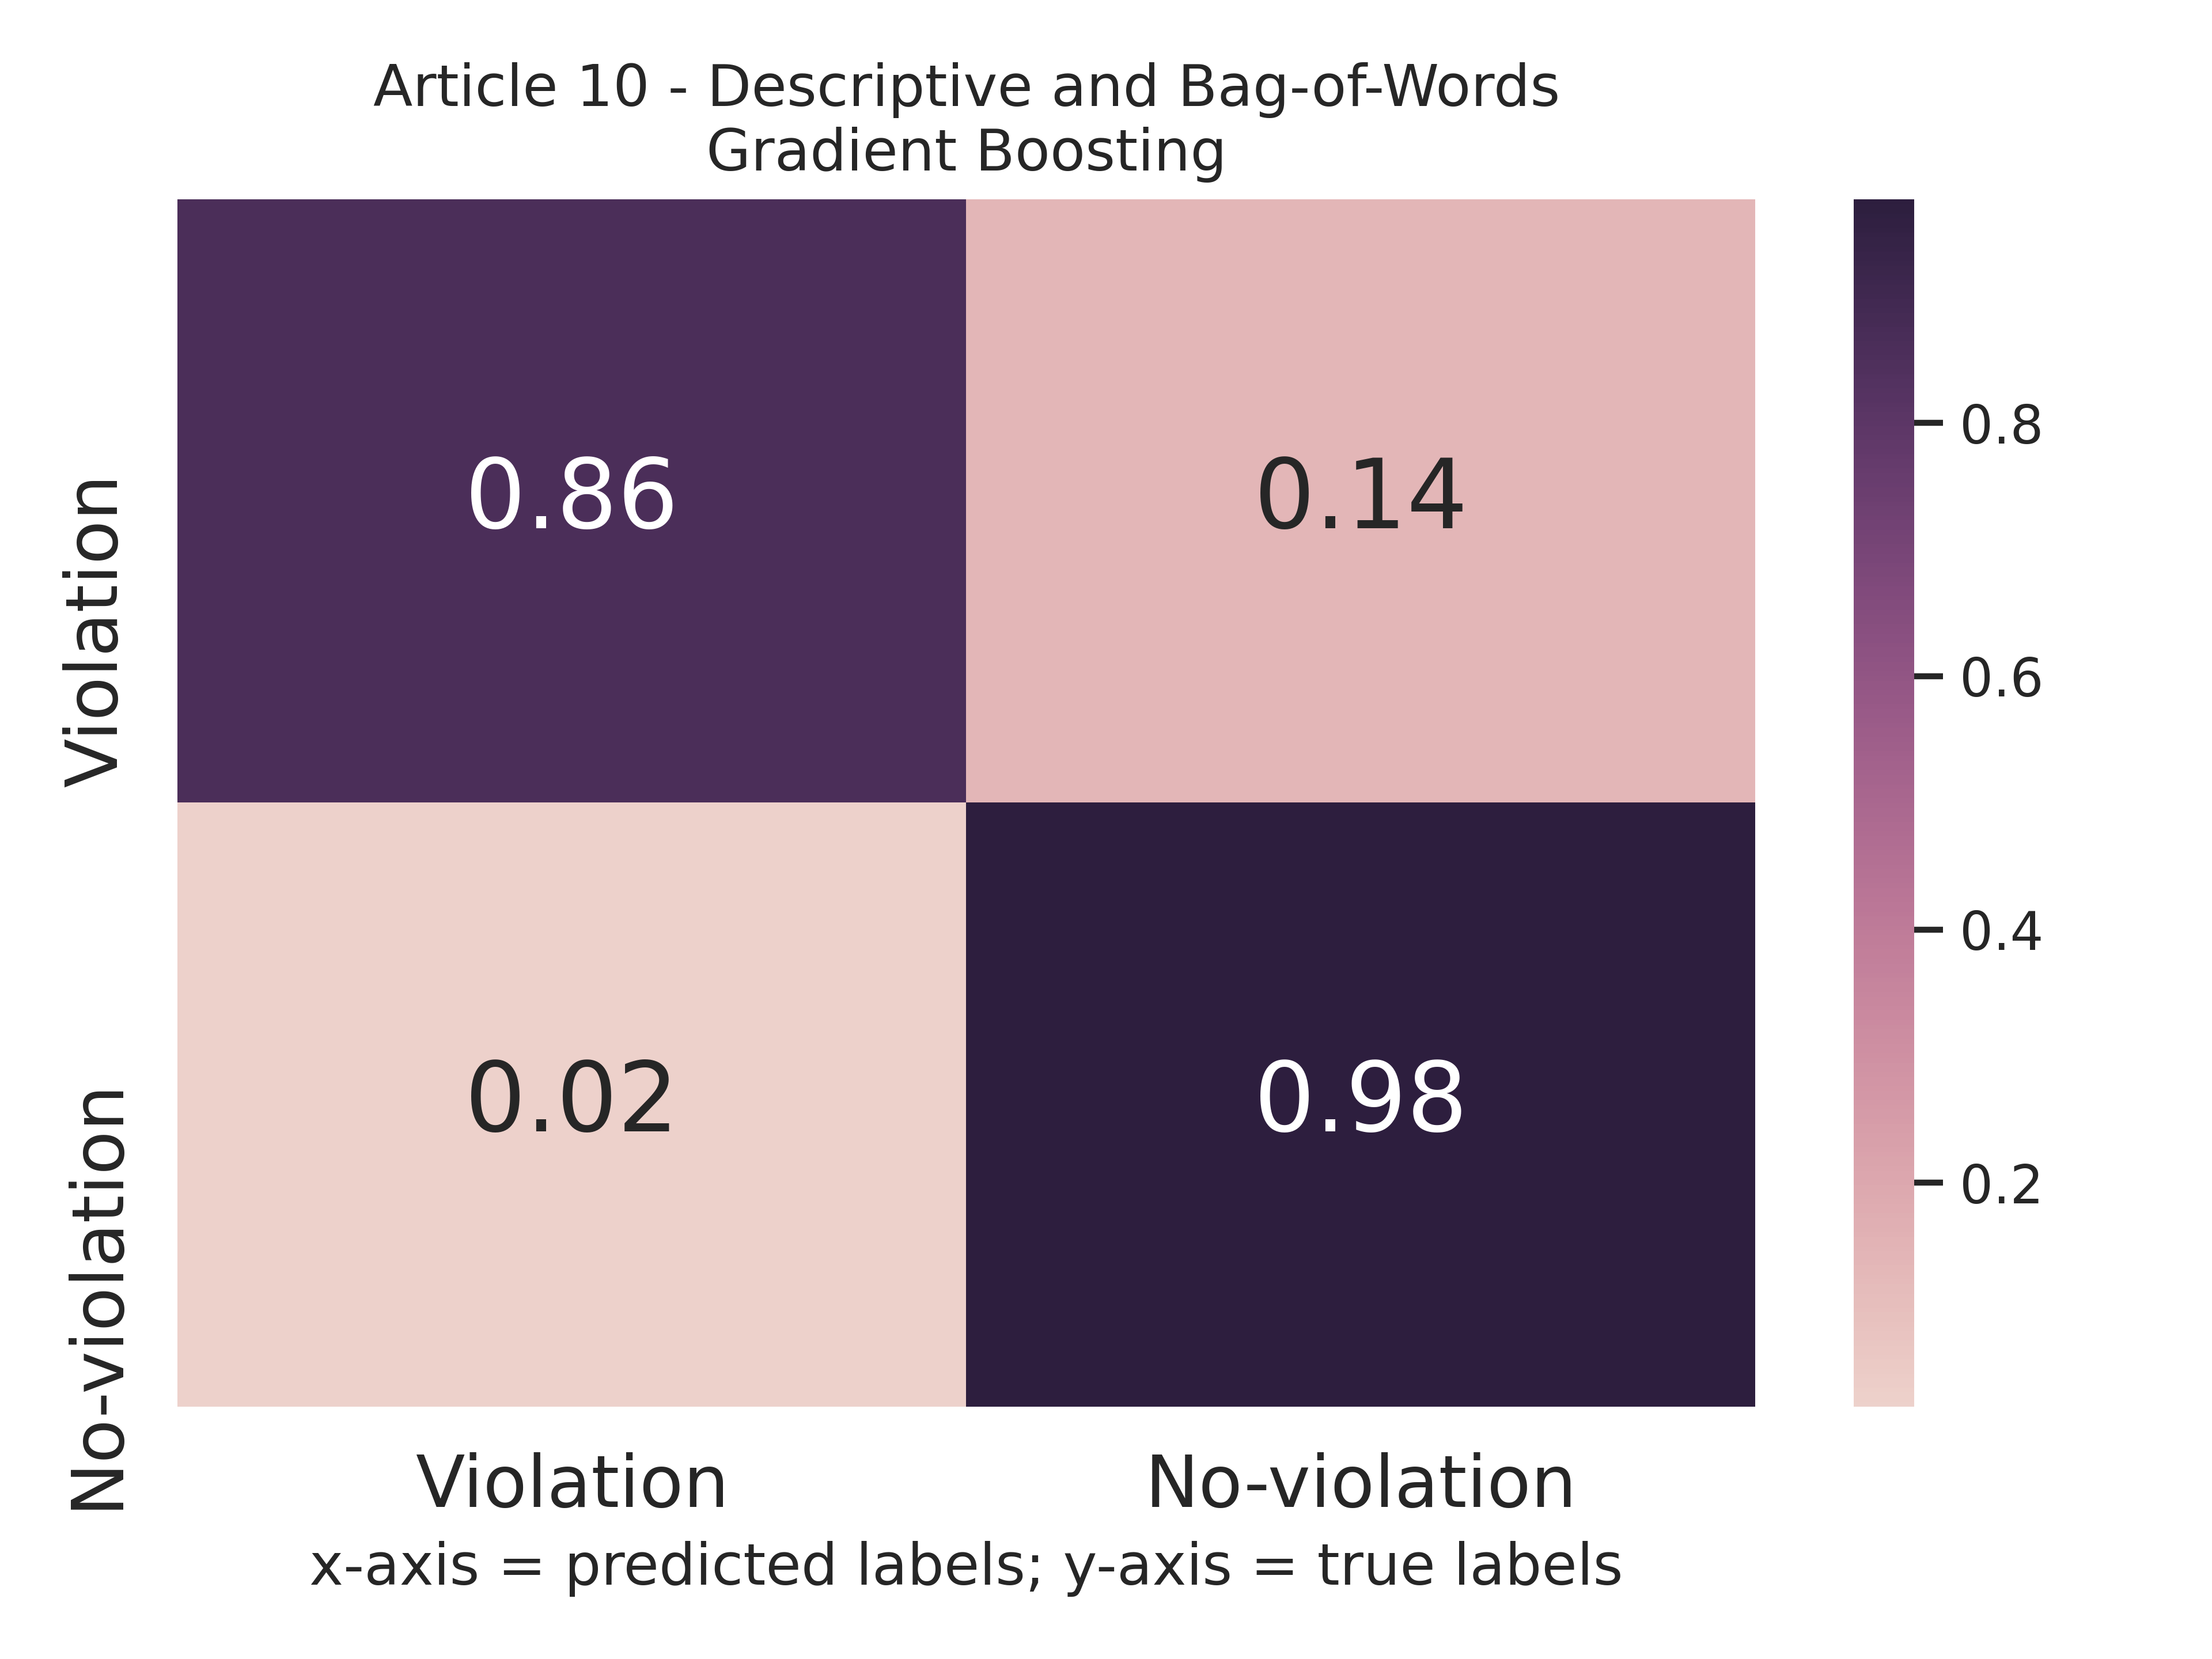
\includegraphics[scale=0.5]{data/analysis/cm/binary_cm_normalized_test_article_10.png}  
\end{figure}
\begin{figure}[!htb]
	\centering
    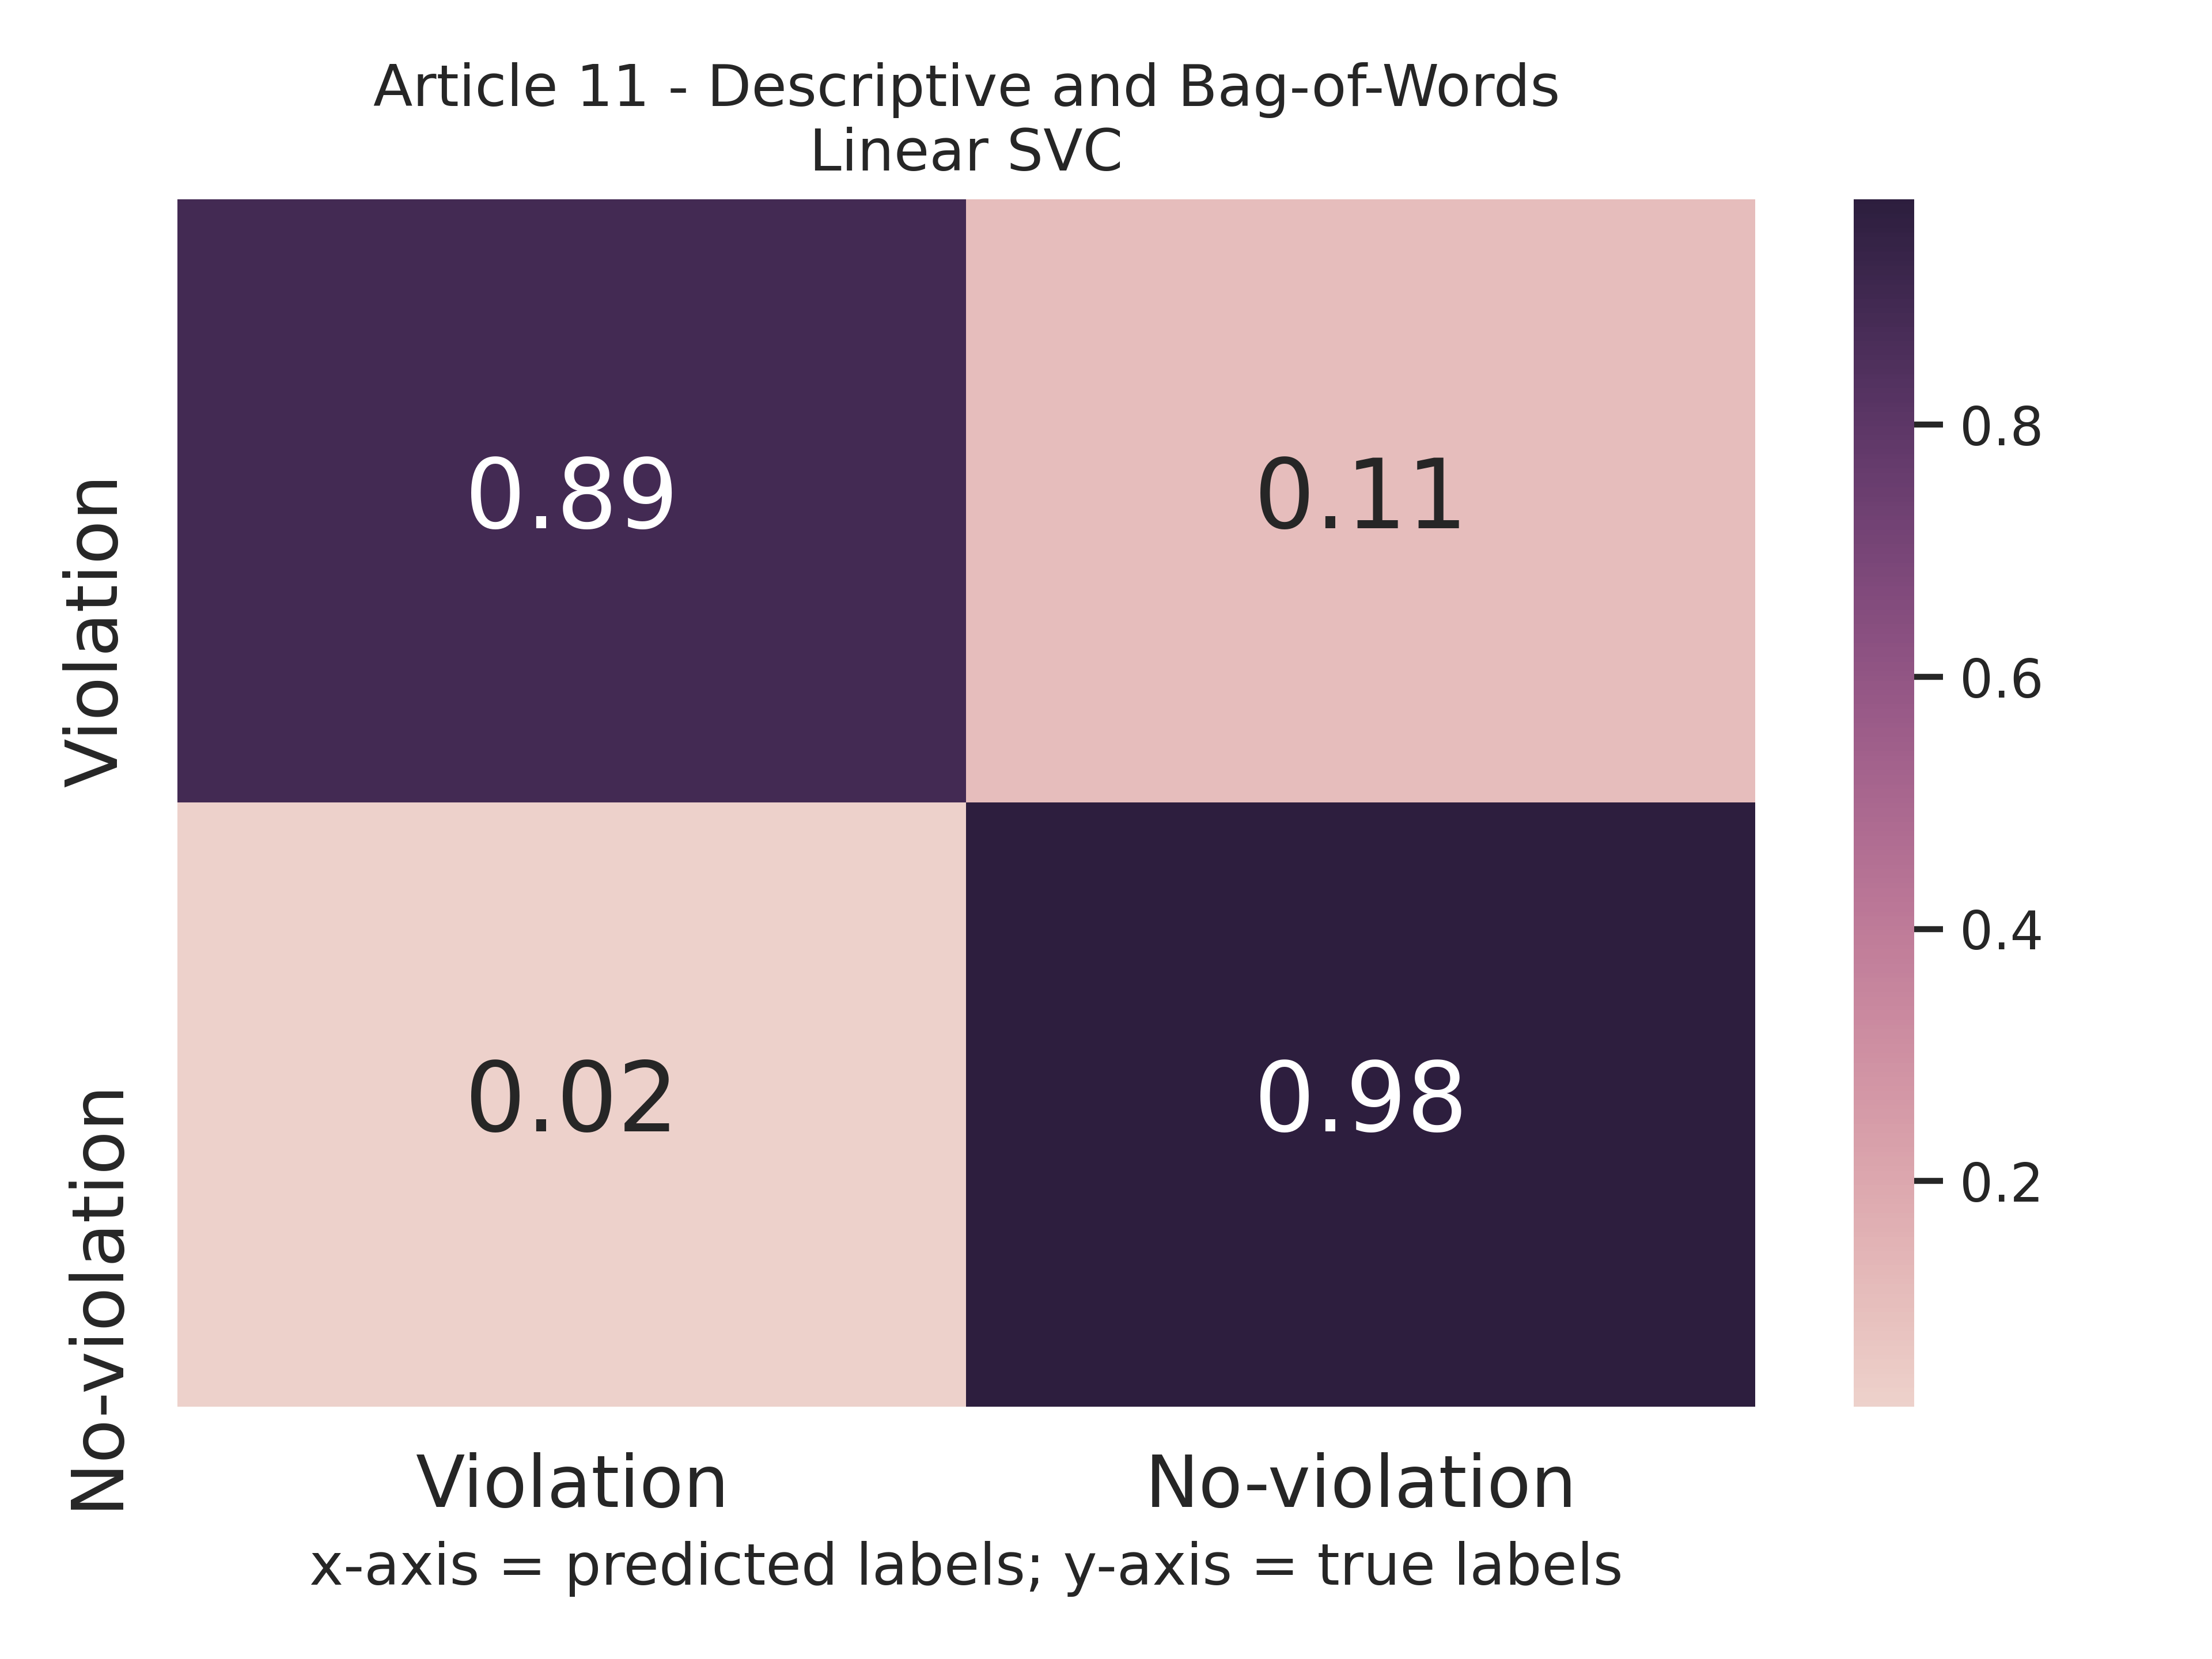
\includegraphics[scale=0.5]{data/analysis/cm/binary_cm_normalized_test_article_11.png}  
\end{figure}
\begin{figure}[!htb]
	\centering
    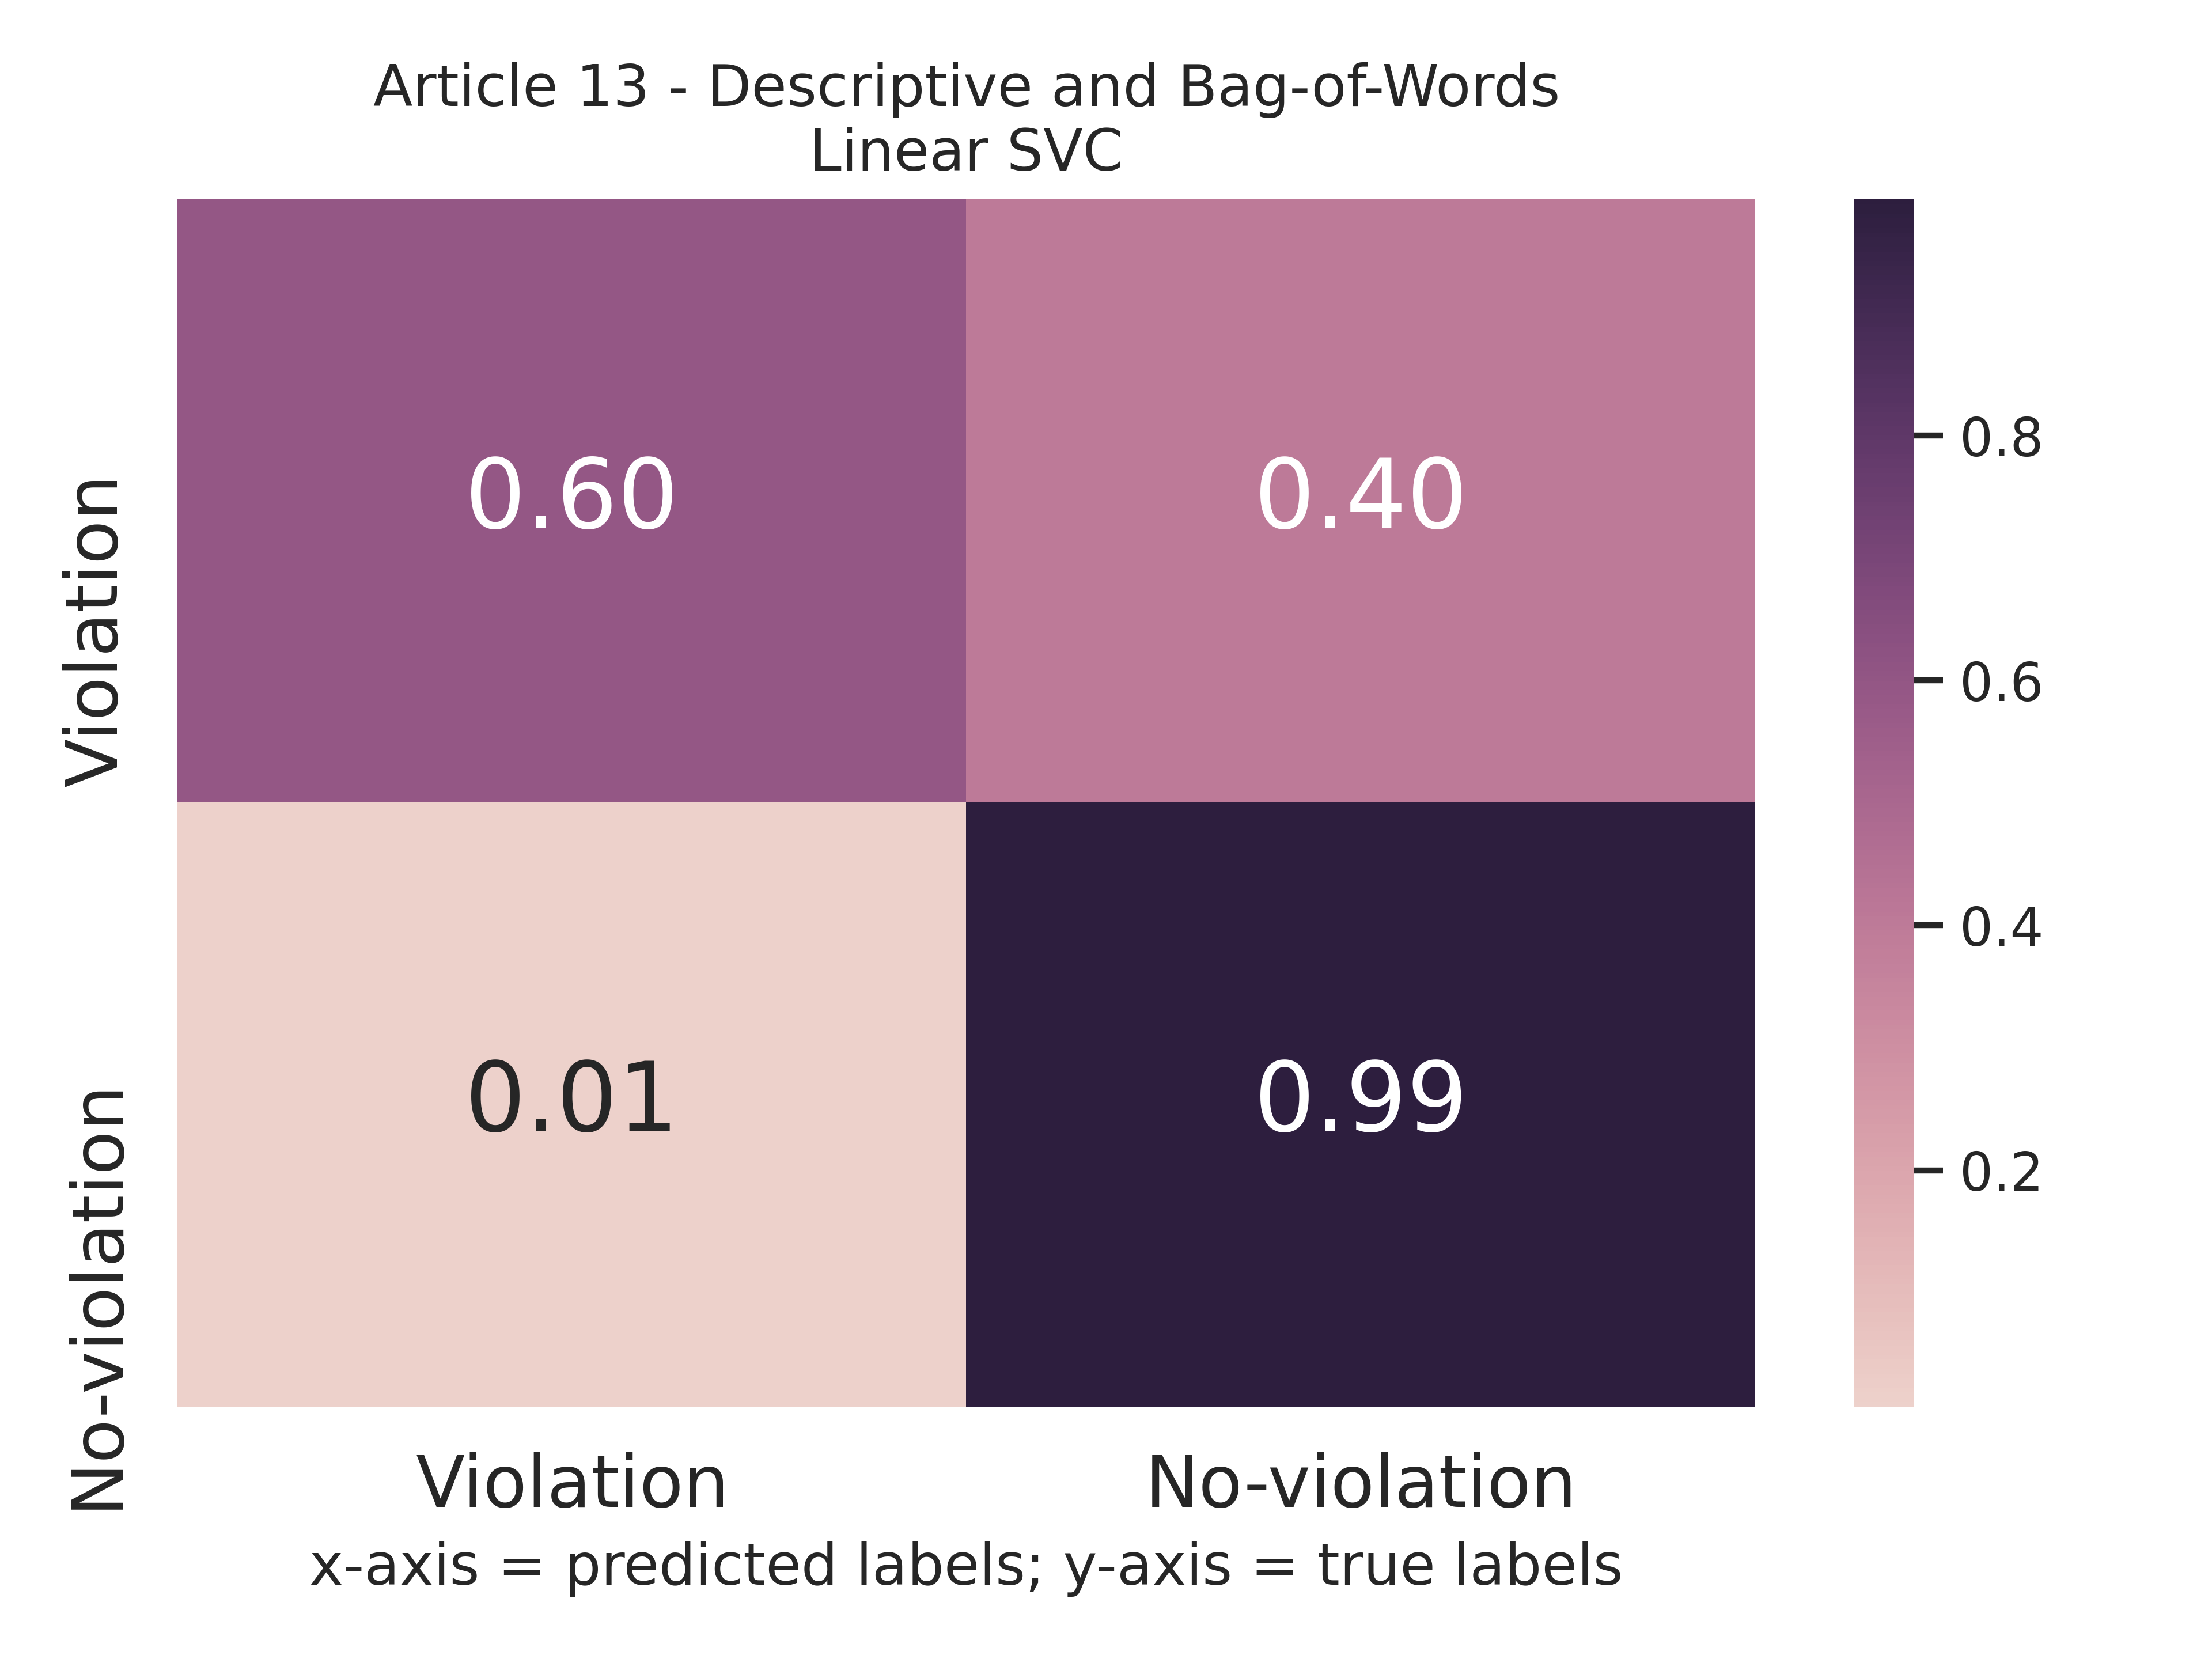
\includegraphics[scale=0.5]{data/analysis/cm/binary_cm_normalized_test_article_13.png}  
\end{figure}
\begin{figure}[!htb]
	\centering
    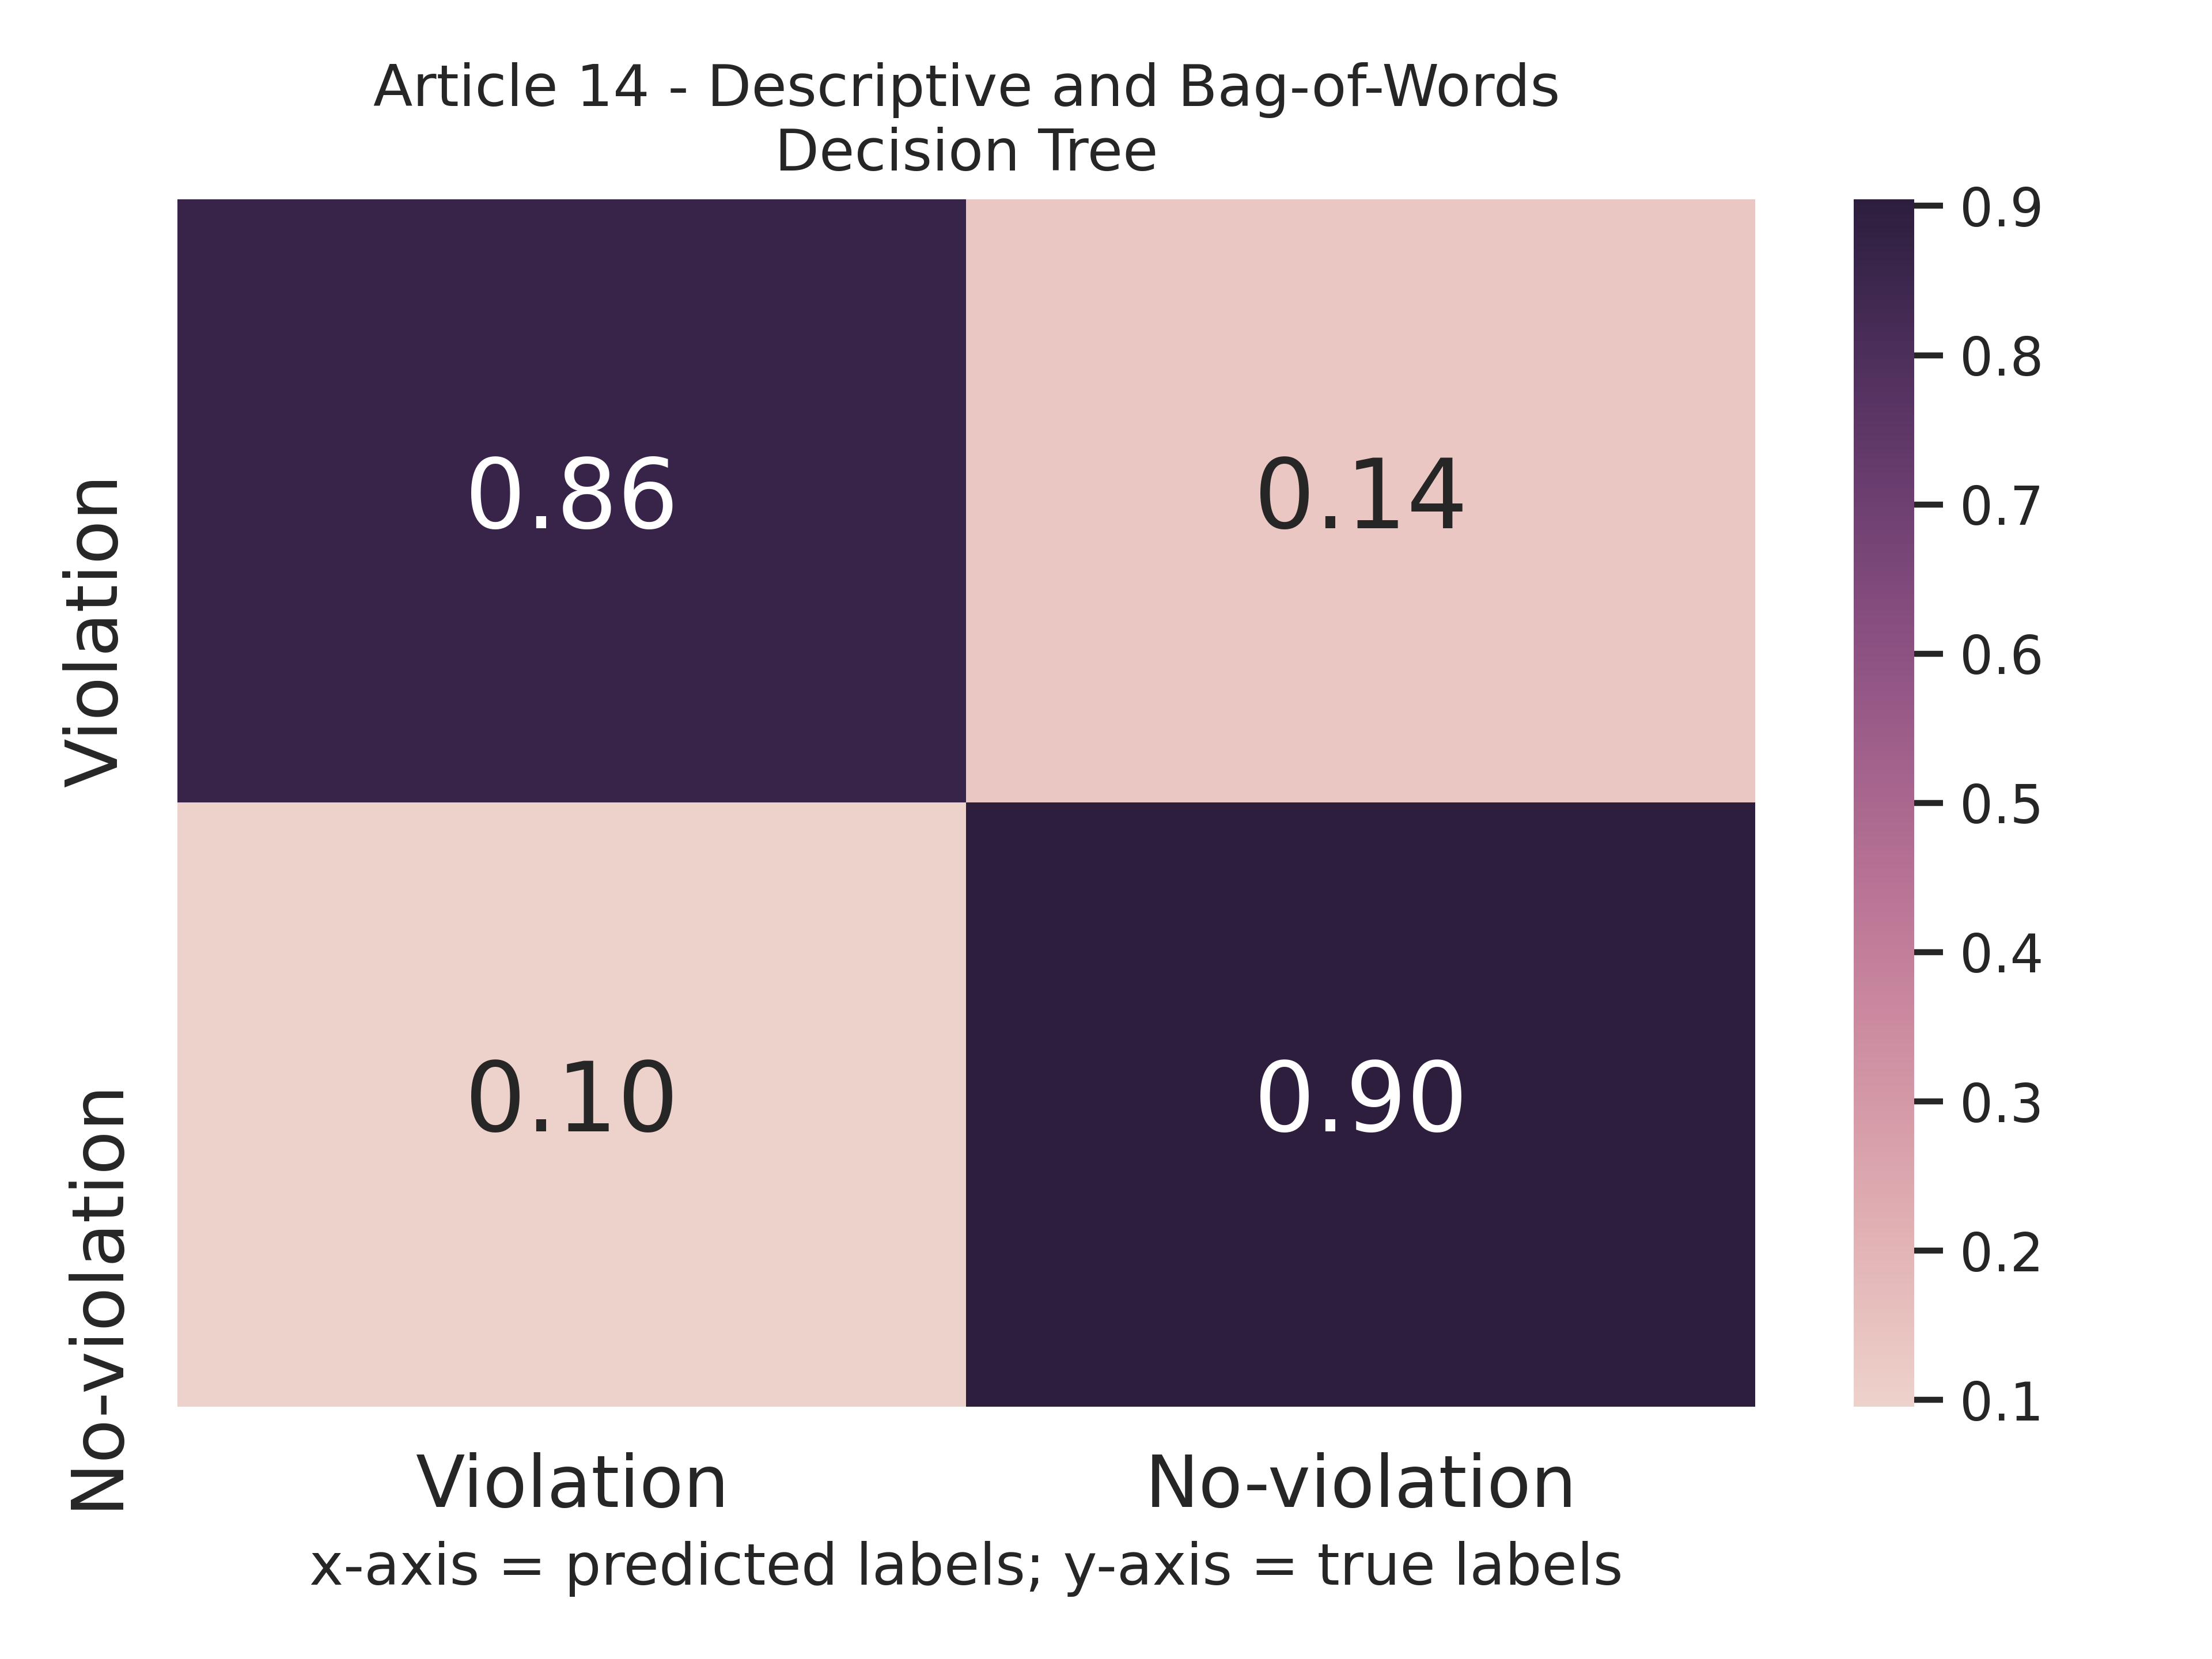
\includegraphics[scale=0.5]{data/analysis/cm/binary_cm_normalized_test_article_14.png}  
\end{figure}
\begin{figure}[!htb]
	\centering
    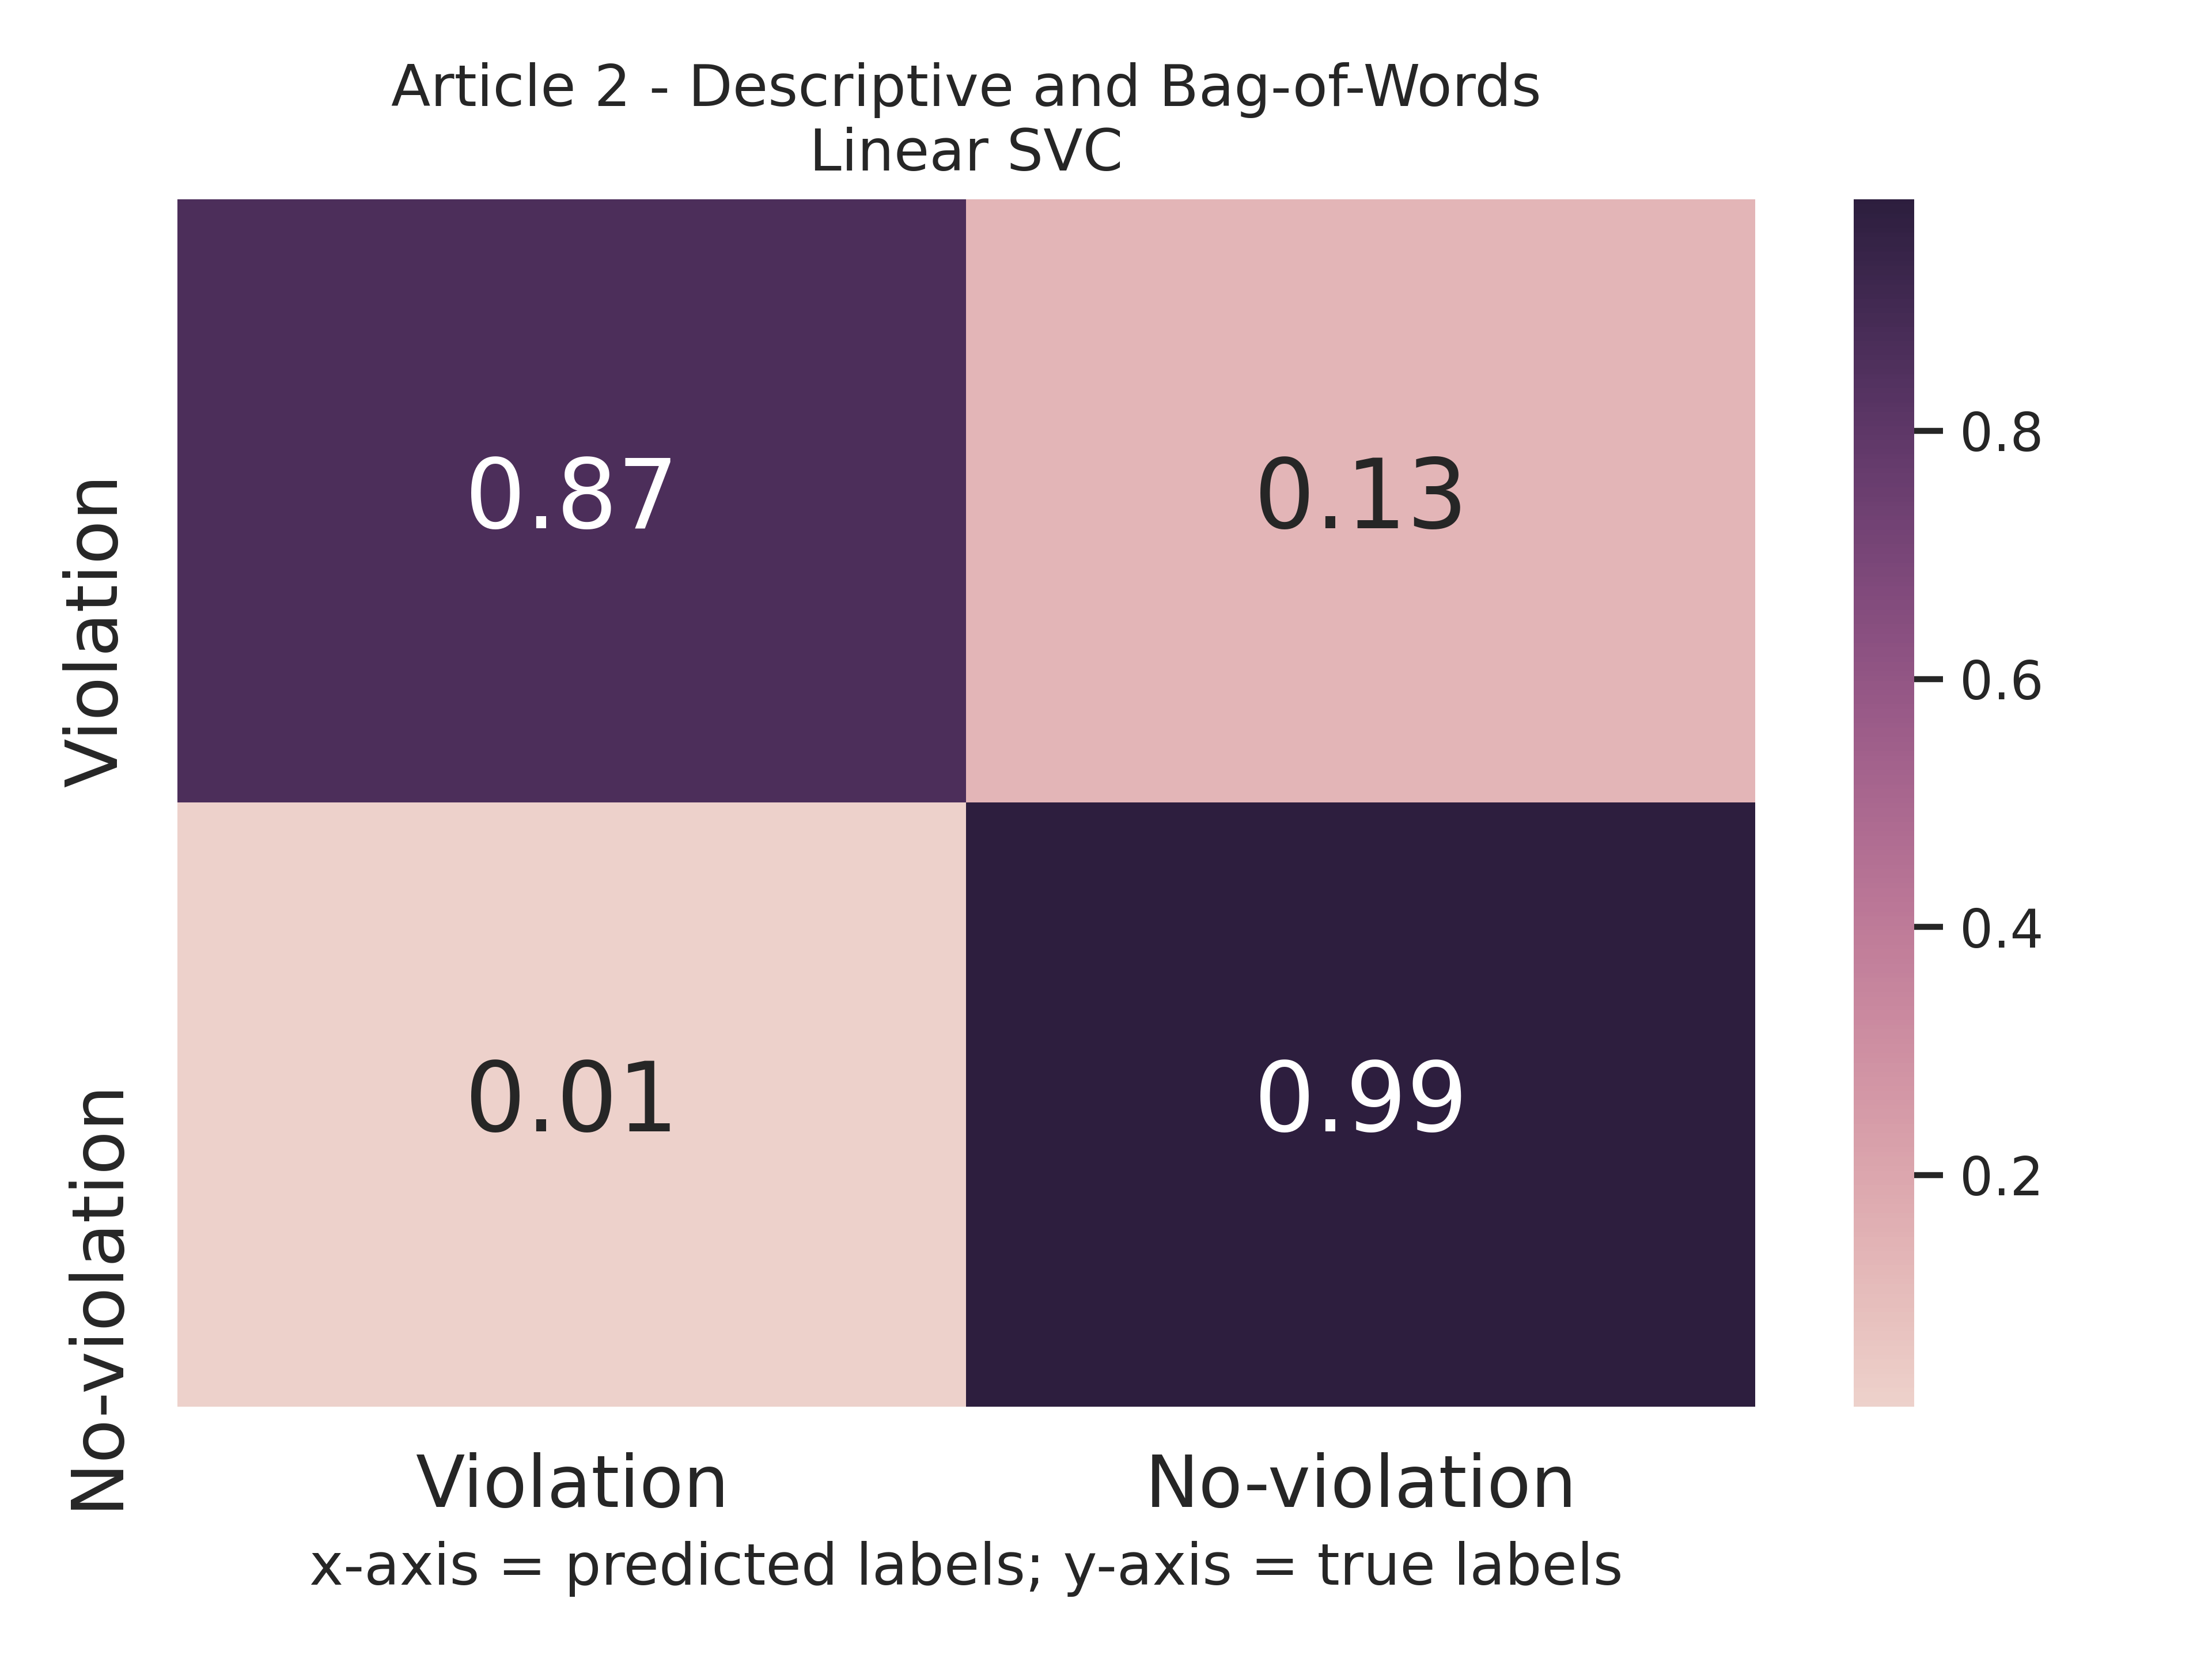
\includegraphics[scale=0.5]{data/analysis/cm/binary_cm_normalized_test_article_2.png}  
\end{figure}
\begin{figure}[!htb]
	\centering
    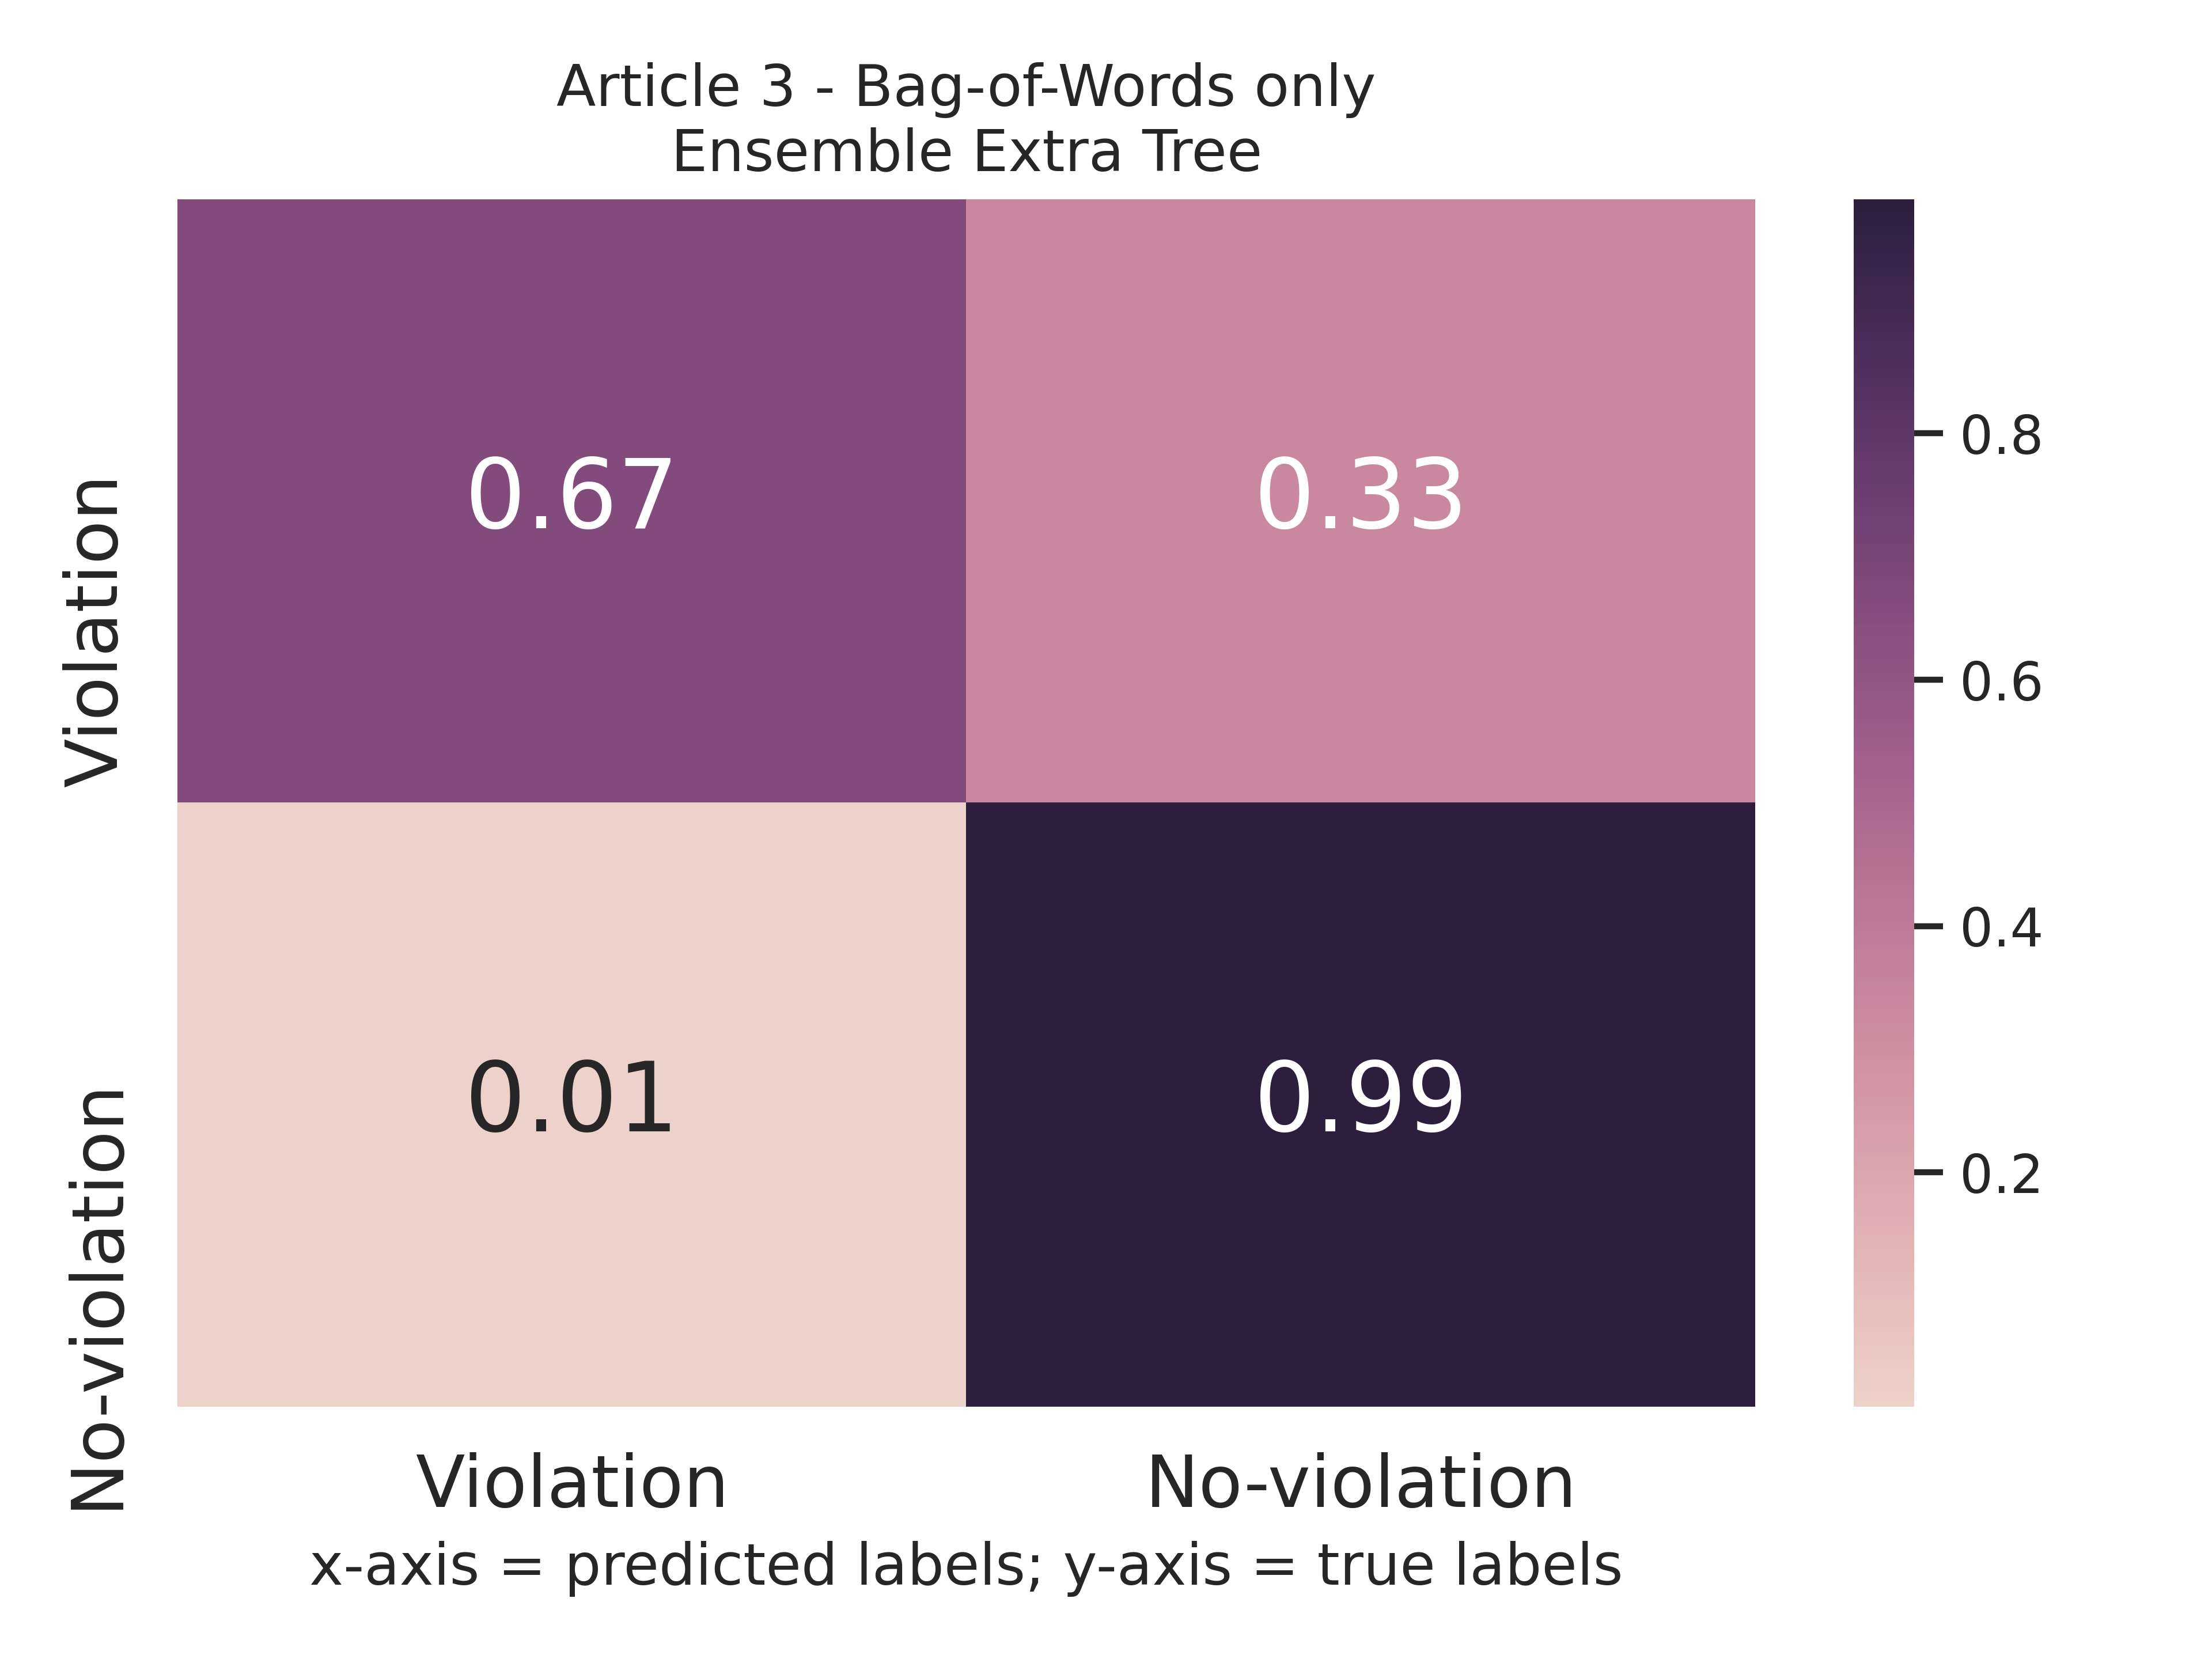
\includegraphics[scale=0.5]{data/analysis/cm/binary_cm_normalized_test_article_3.png}  
\end{figure}
\begin{figure}[!htb]
	\centering
    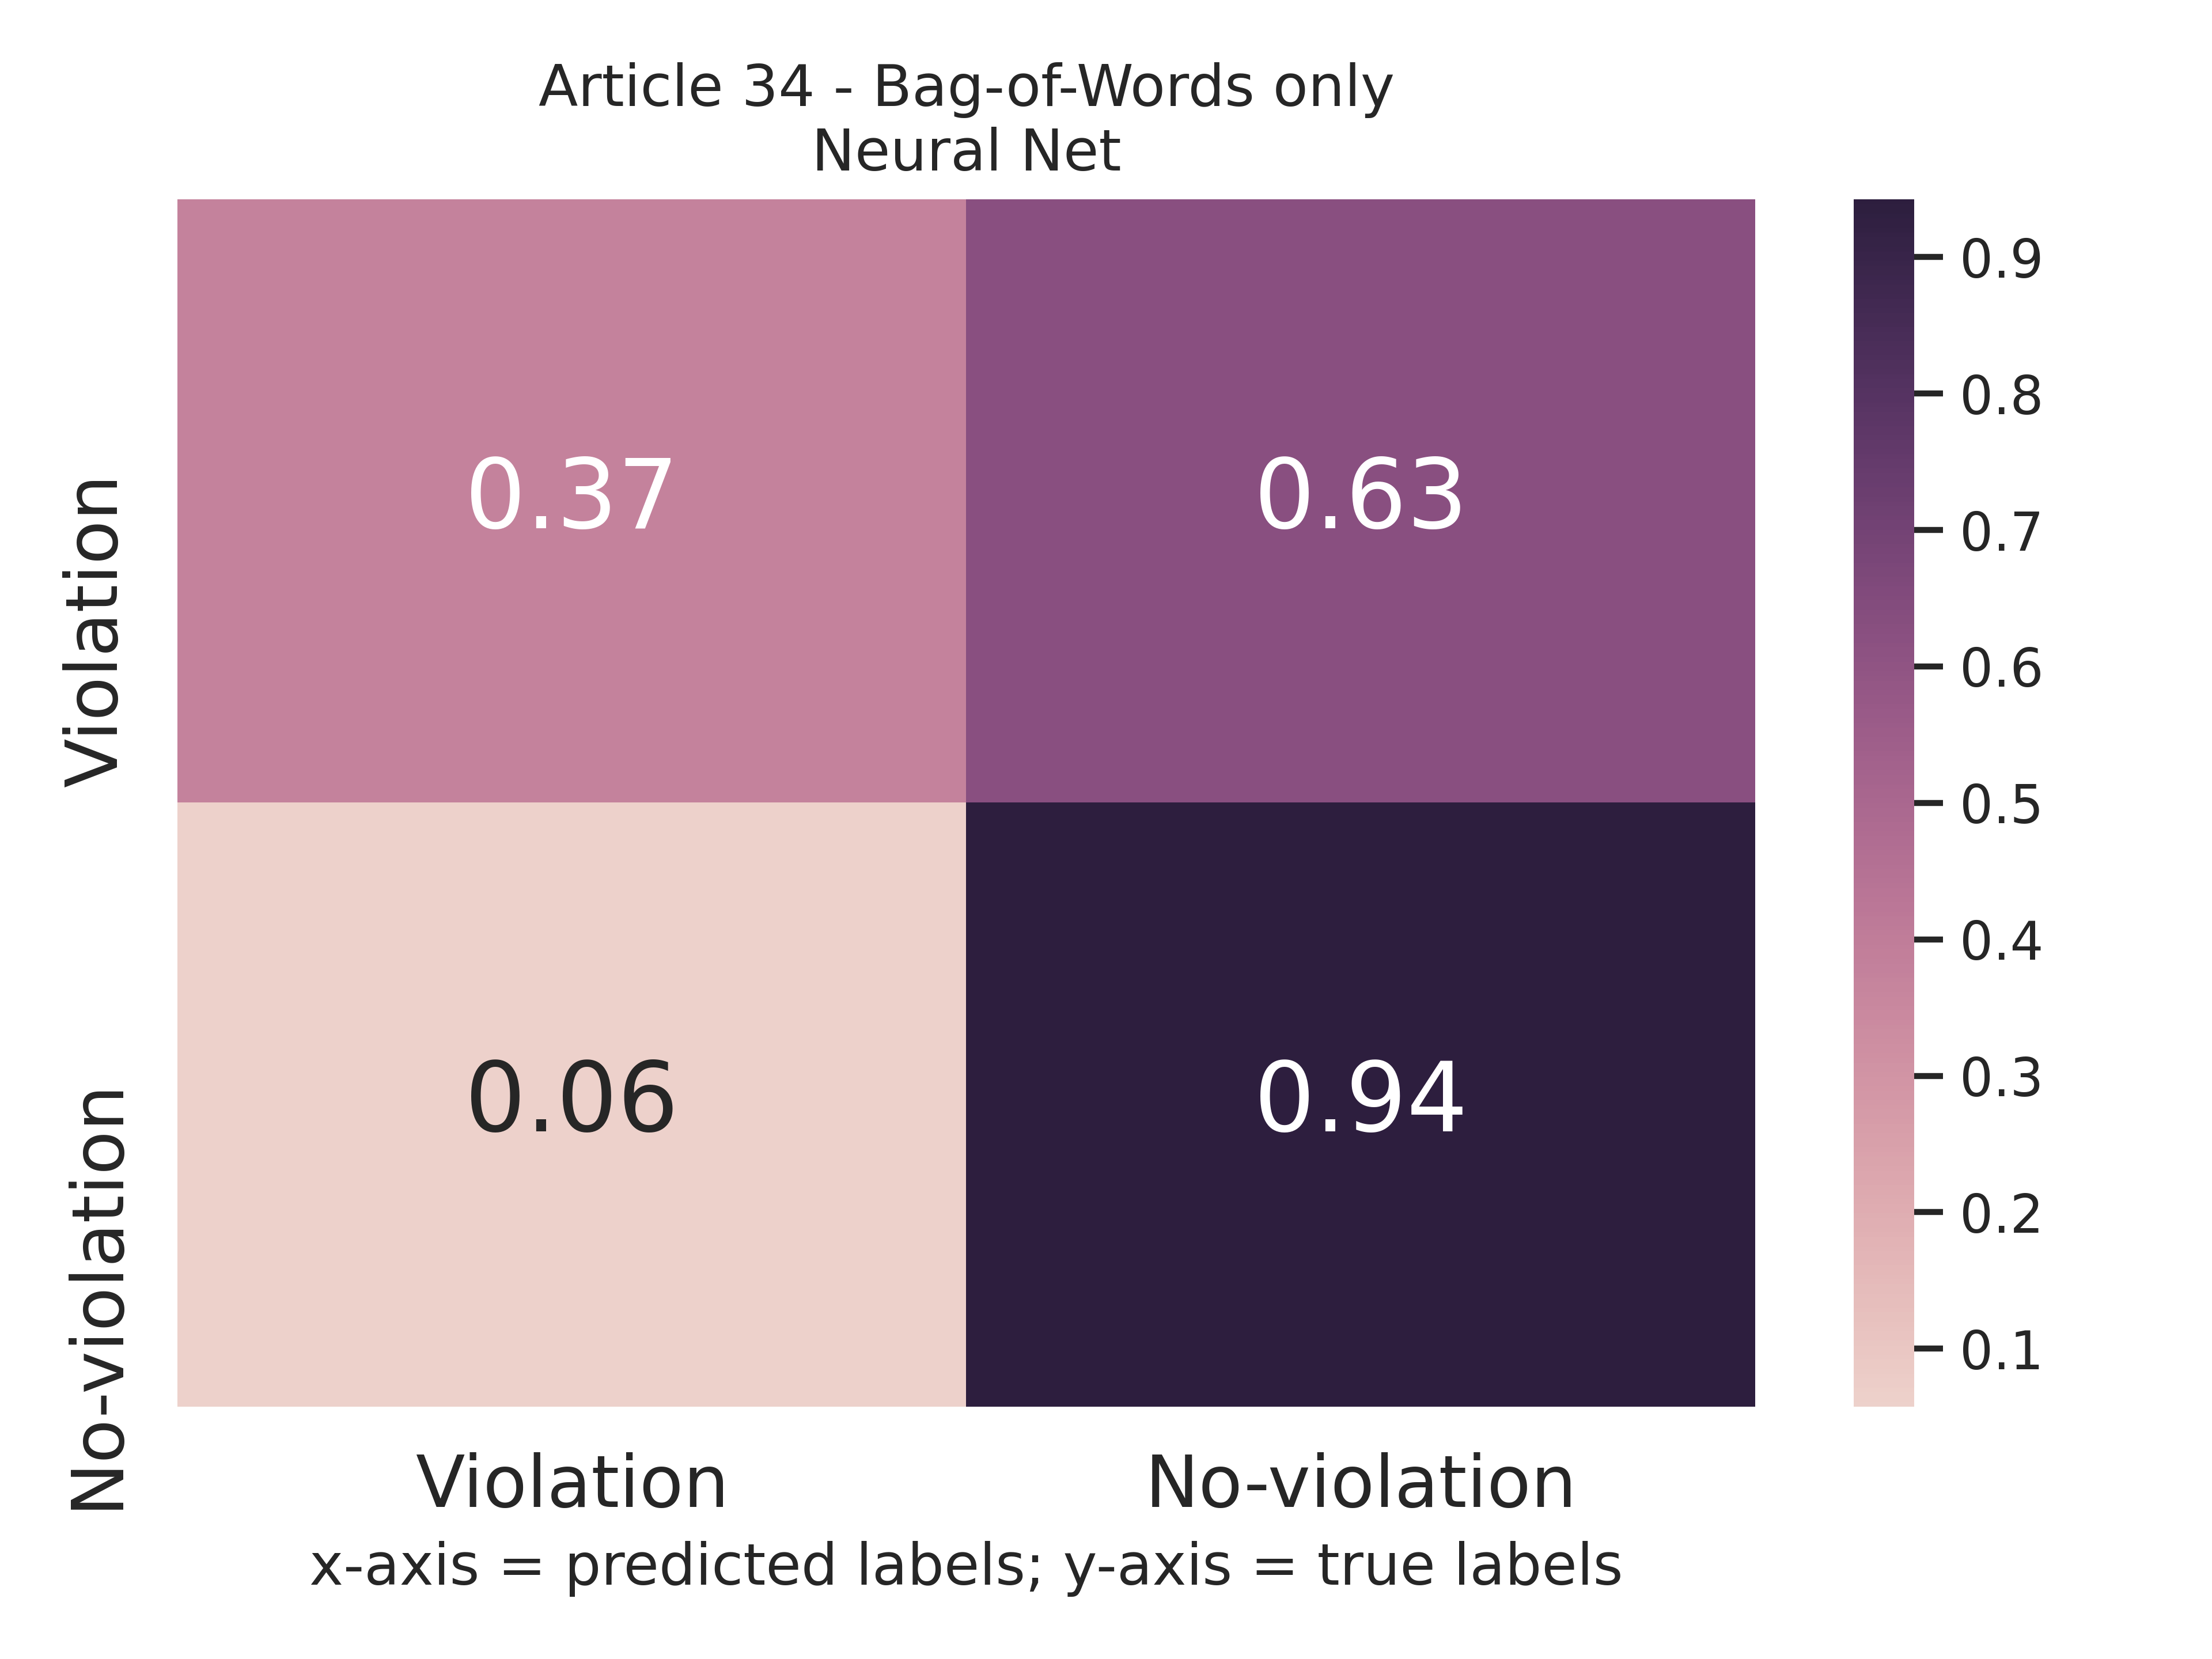
\includegraphics[scale=0.5]{data/analysis/cm/binary_cm_normalized_test_article_34.png}  
\end{figure}
\begin{figure}[!htb]
	\centering
    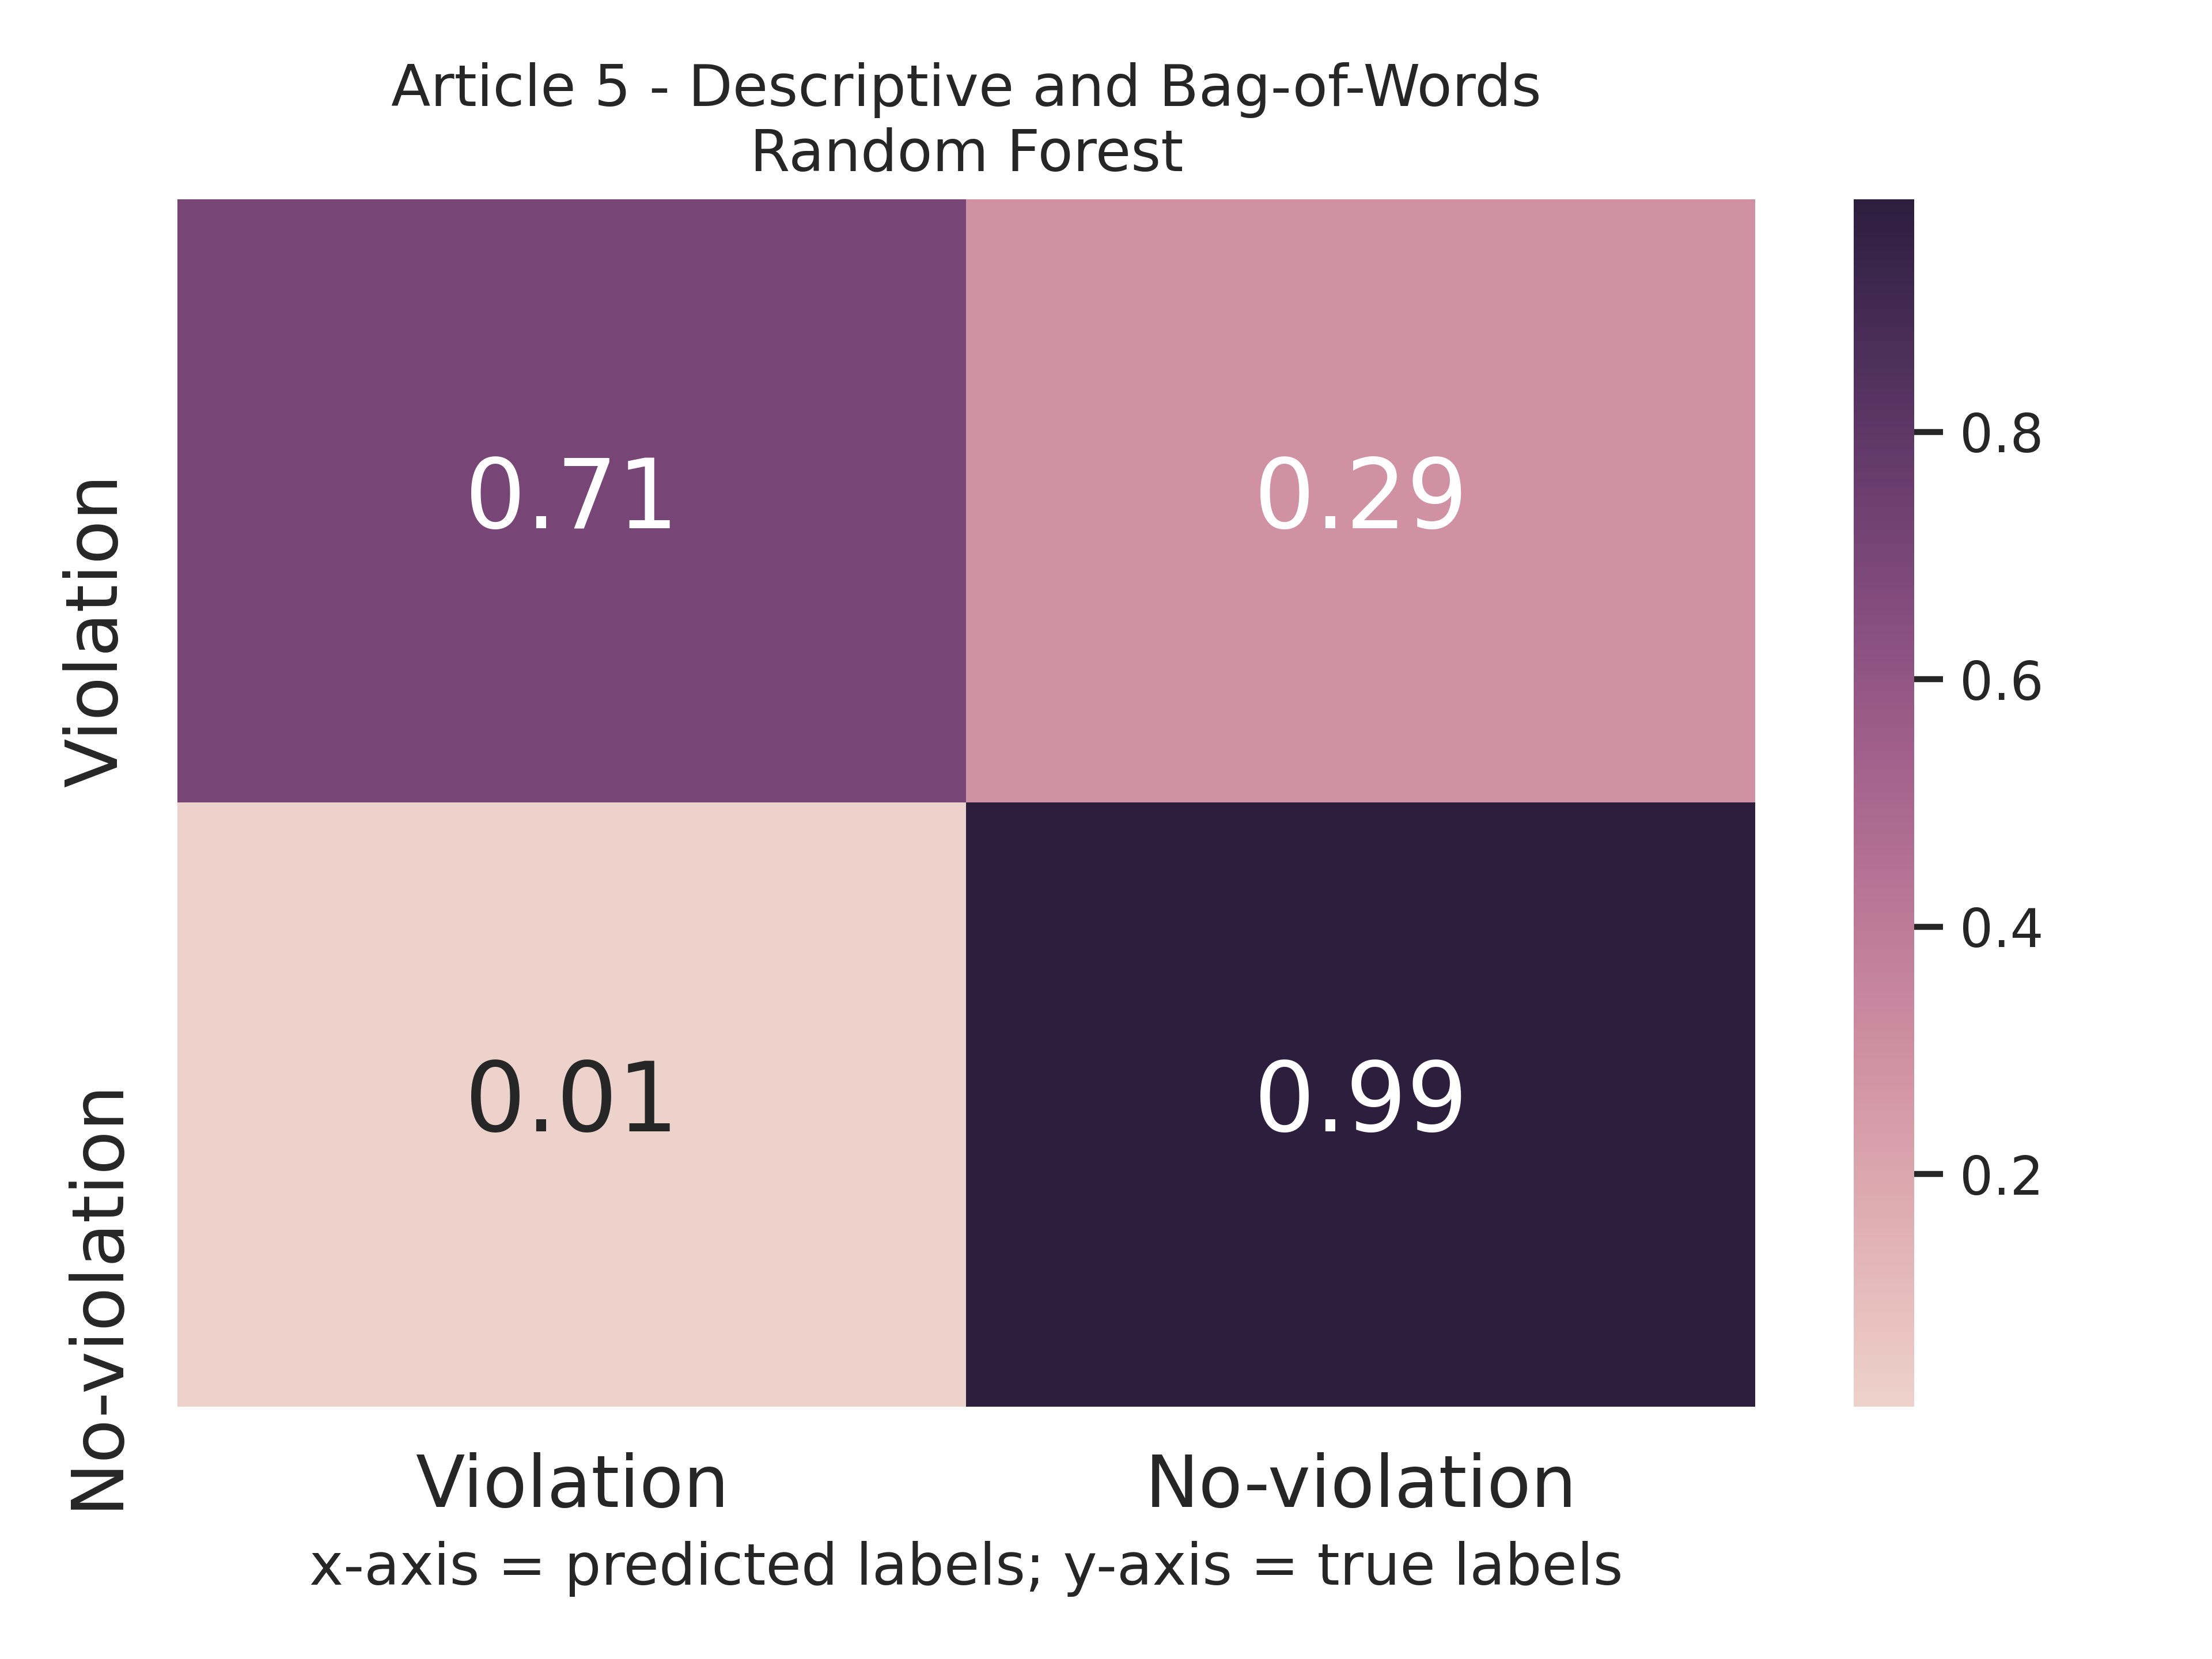
\includegraphics[scale=0.5]{data/analysis/cm/binary_cm_normalized_test_article_5.png}  
\end{figure}
\begin{figure}[!htb]
	\centering
    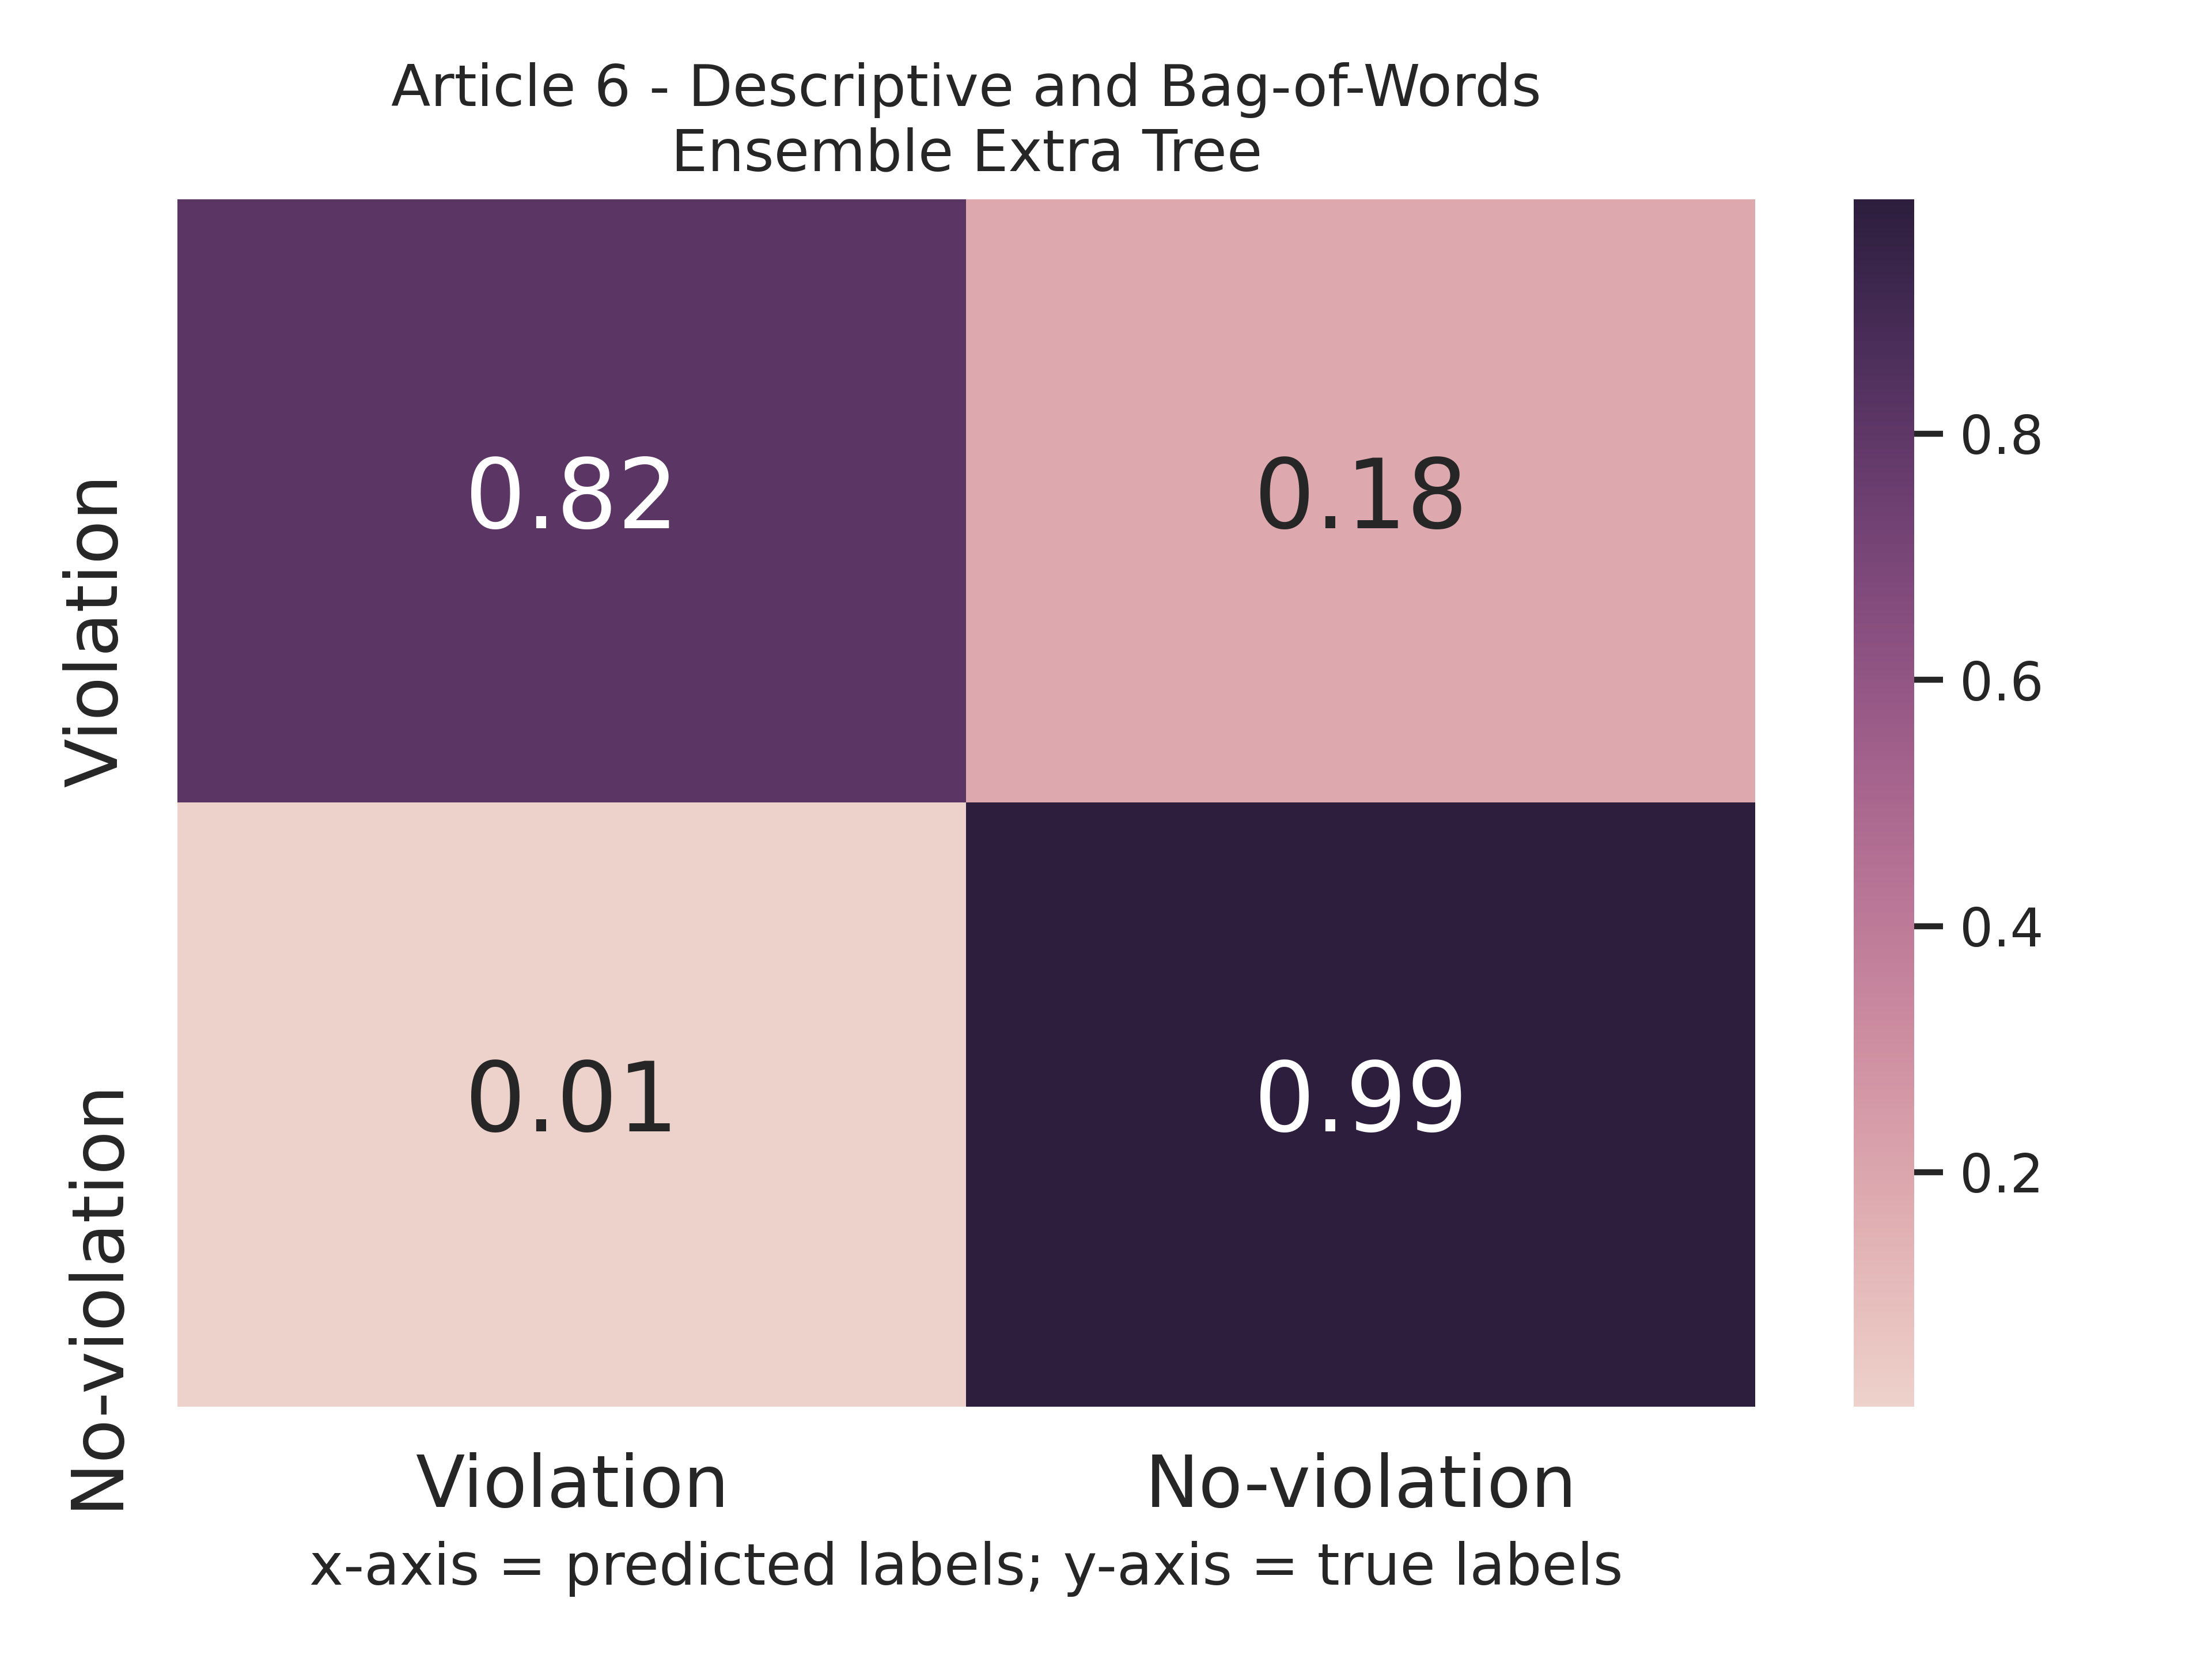
\includegraphics[scale=0.5]{data/analysis/cm/binary_cm_normalized_test_article_6.png}  
\end{figure}
\begin{figure}[!htb]
	\centering
    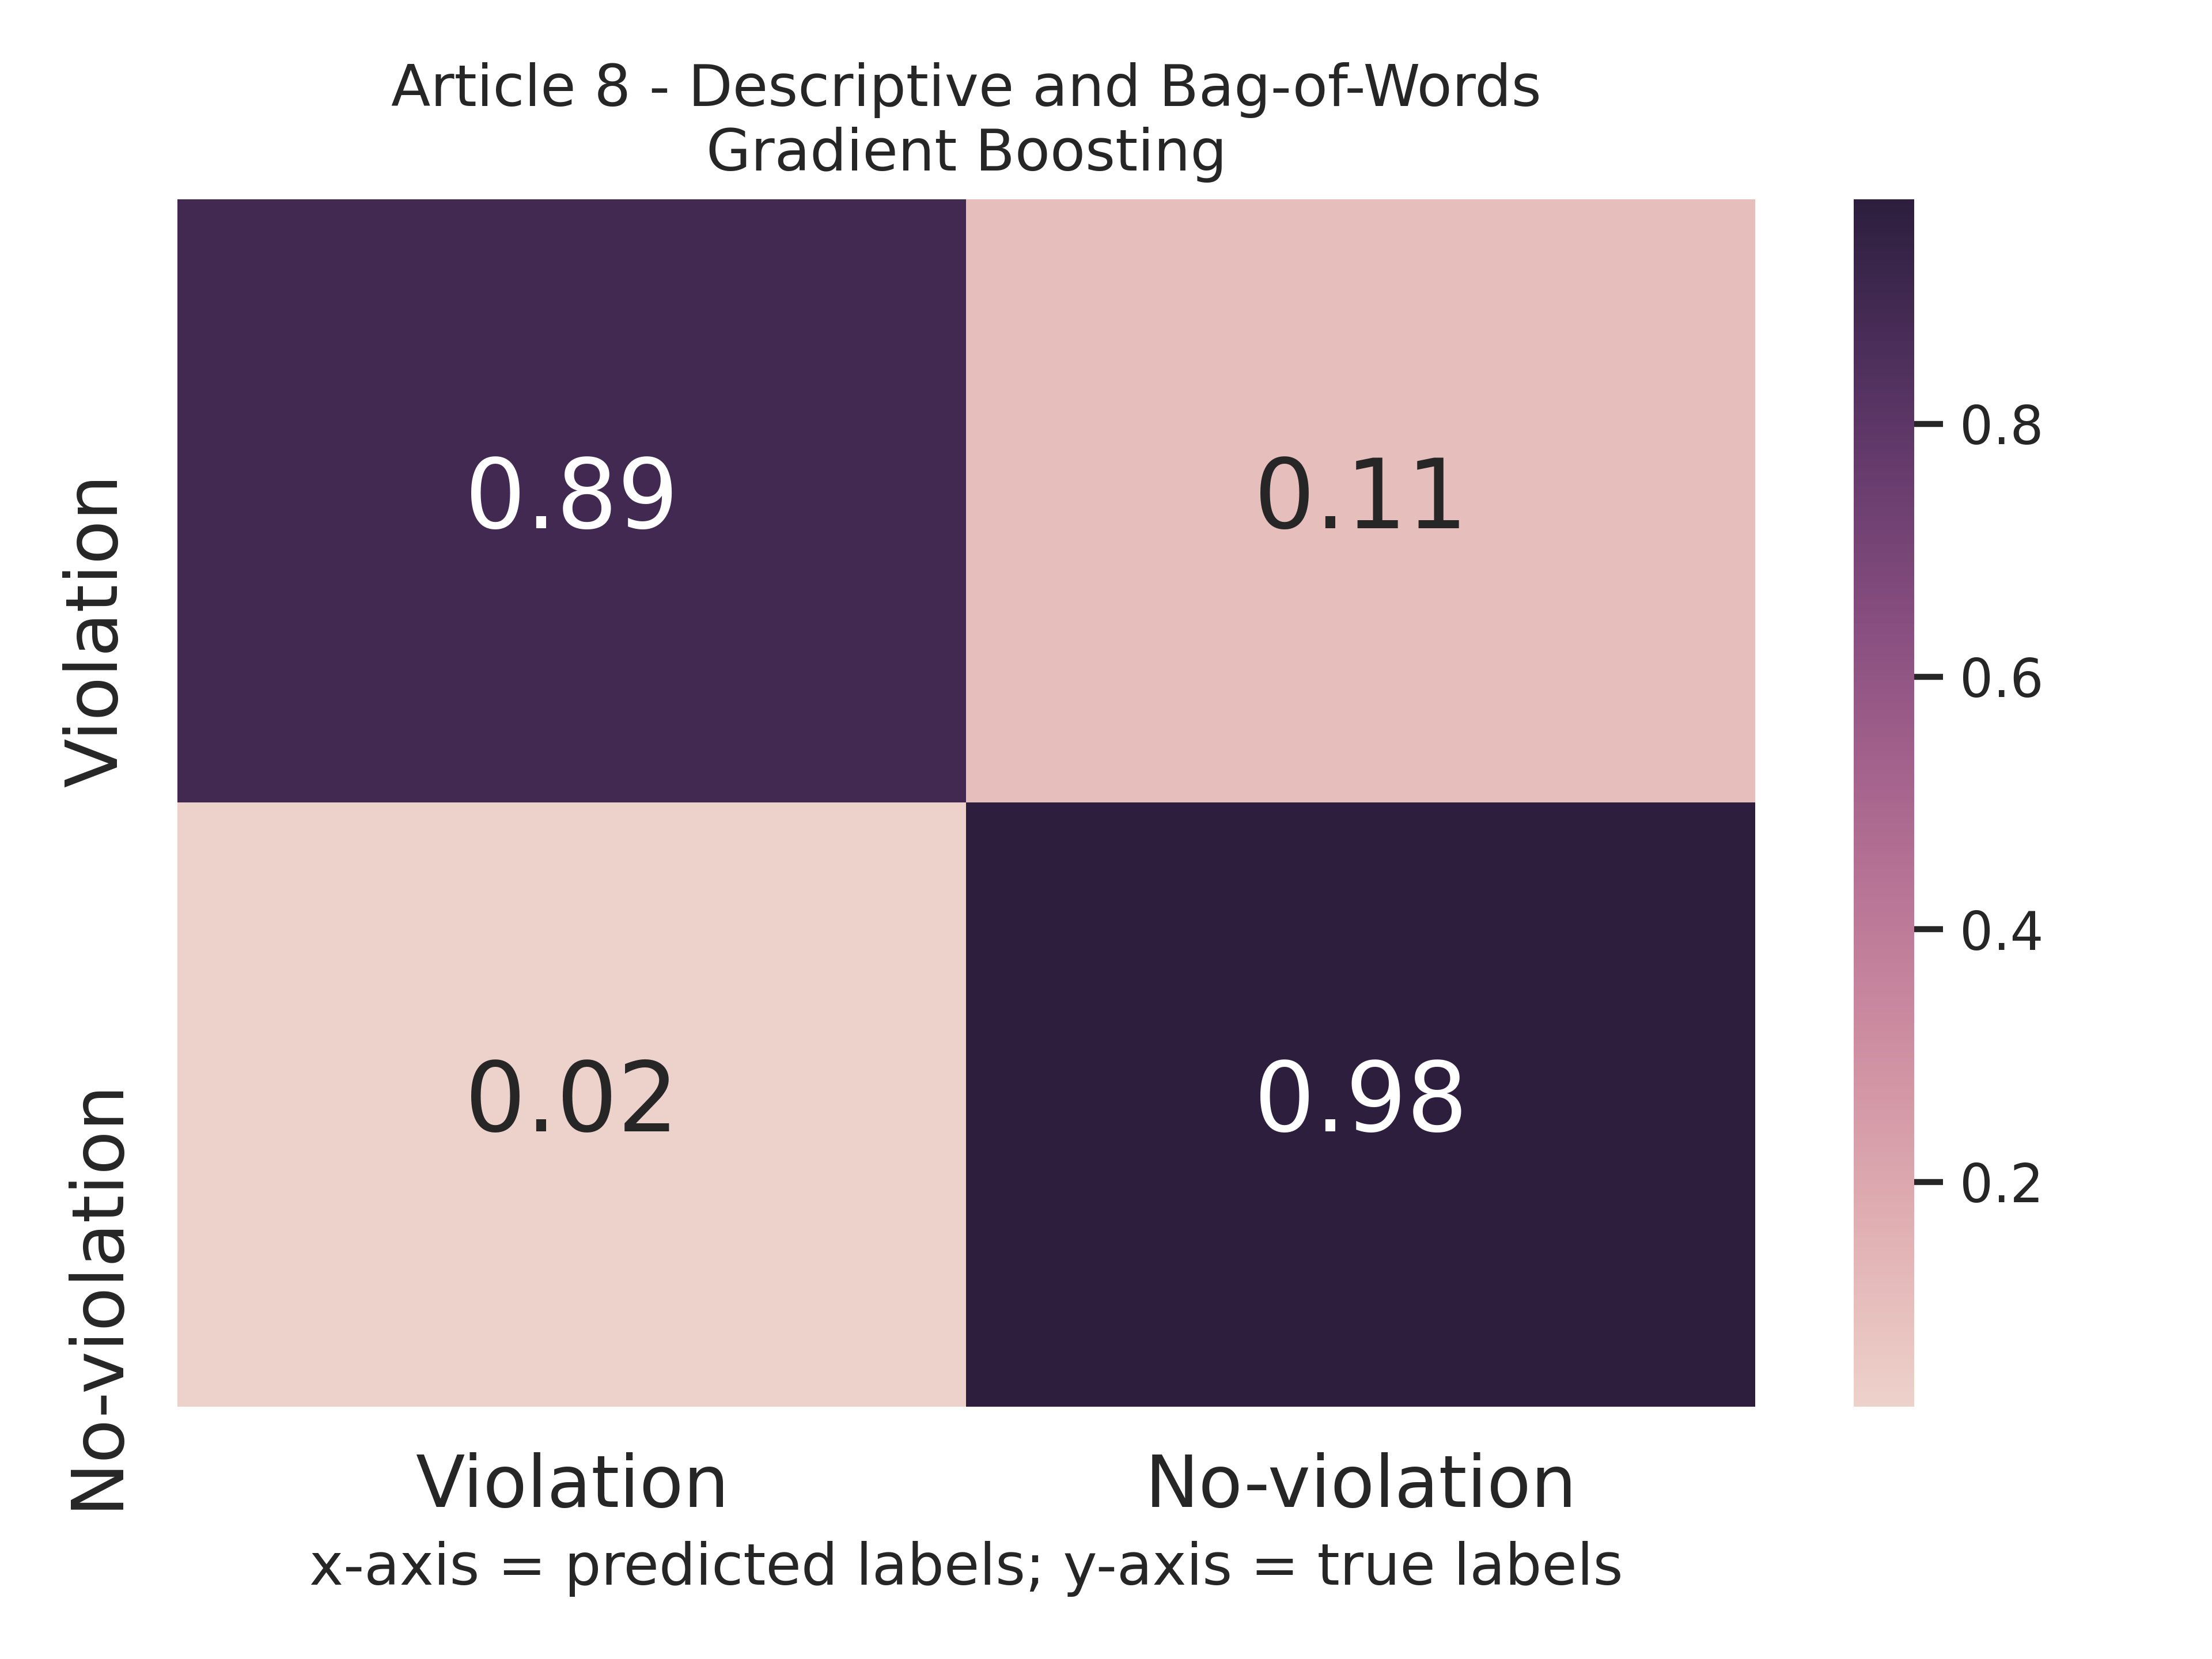
\includegraphics[scale=0.5]{data/analysis/cm/binary_cm_normalized_test_article_8.png}  
\end{figure}
\begin{figure}[!htb]
	\centering
    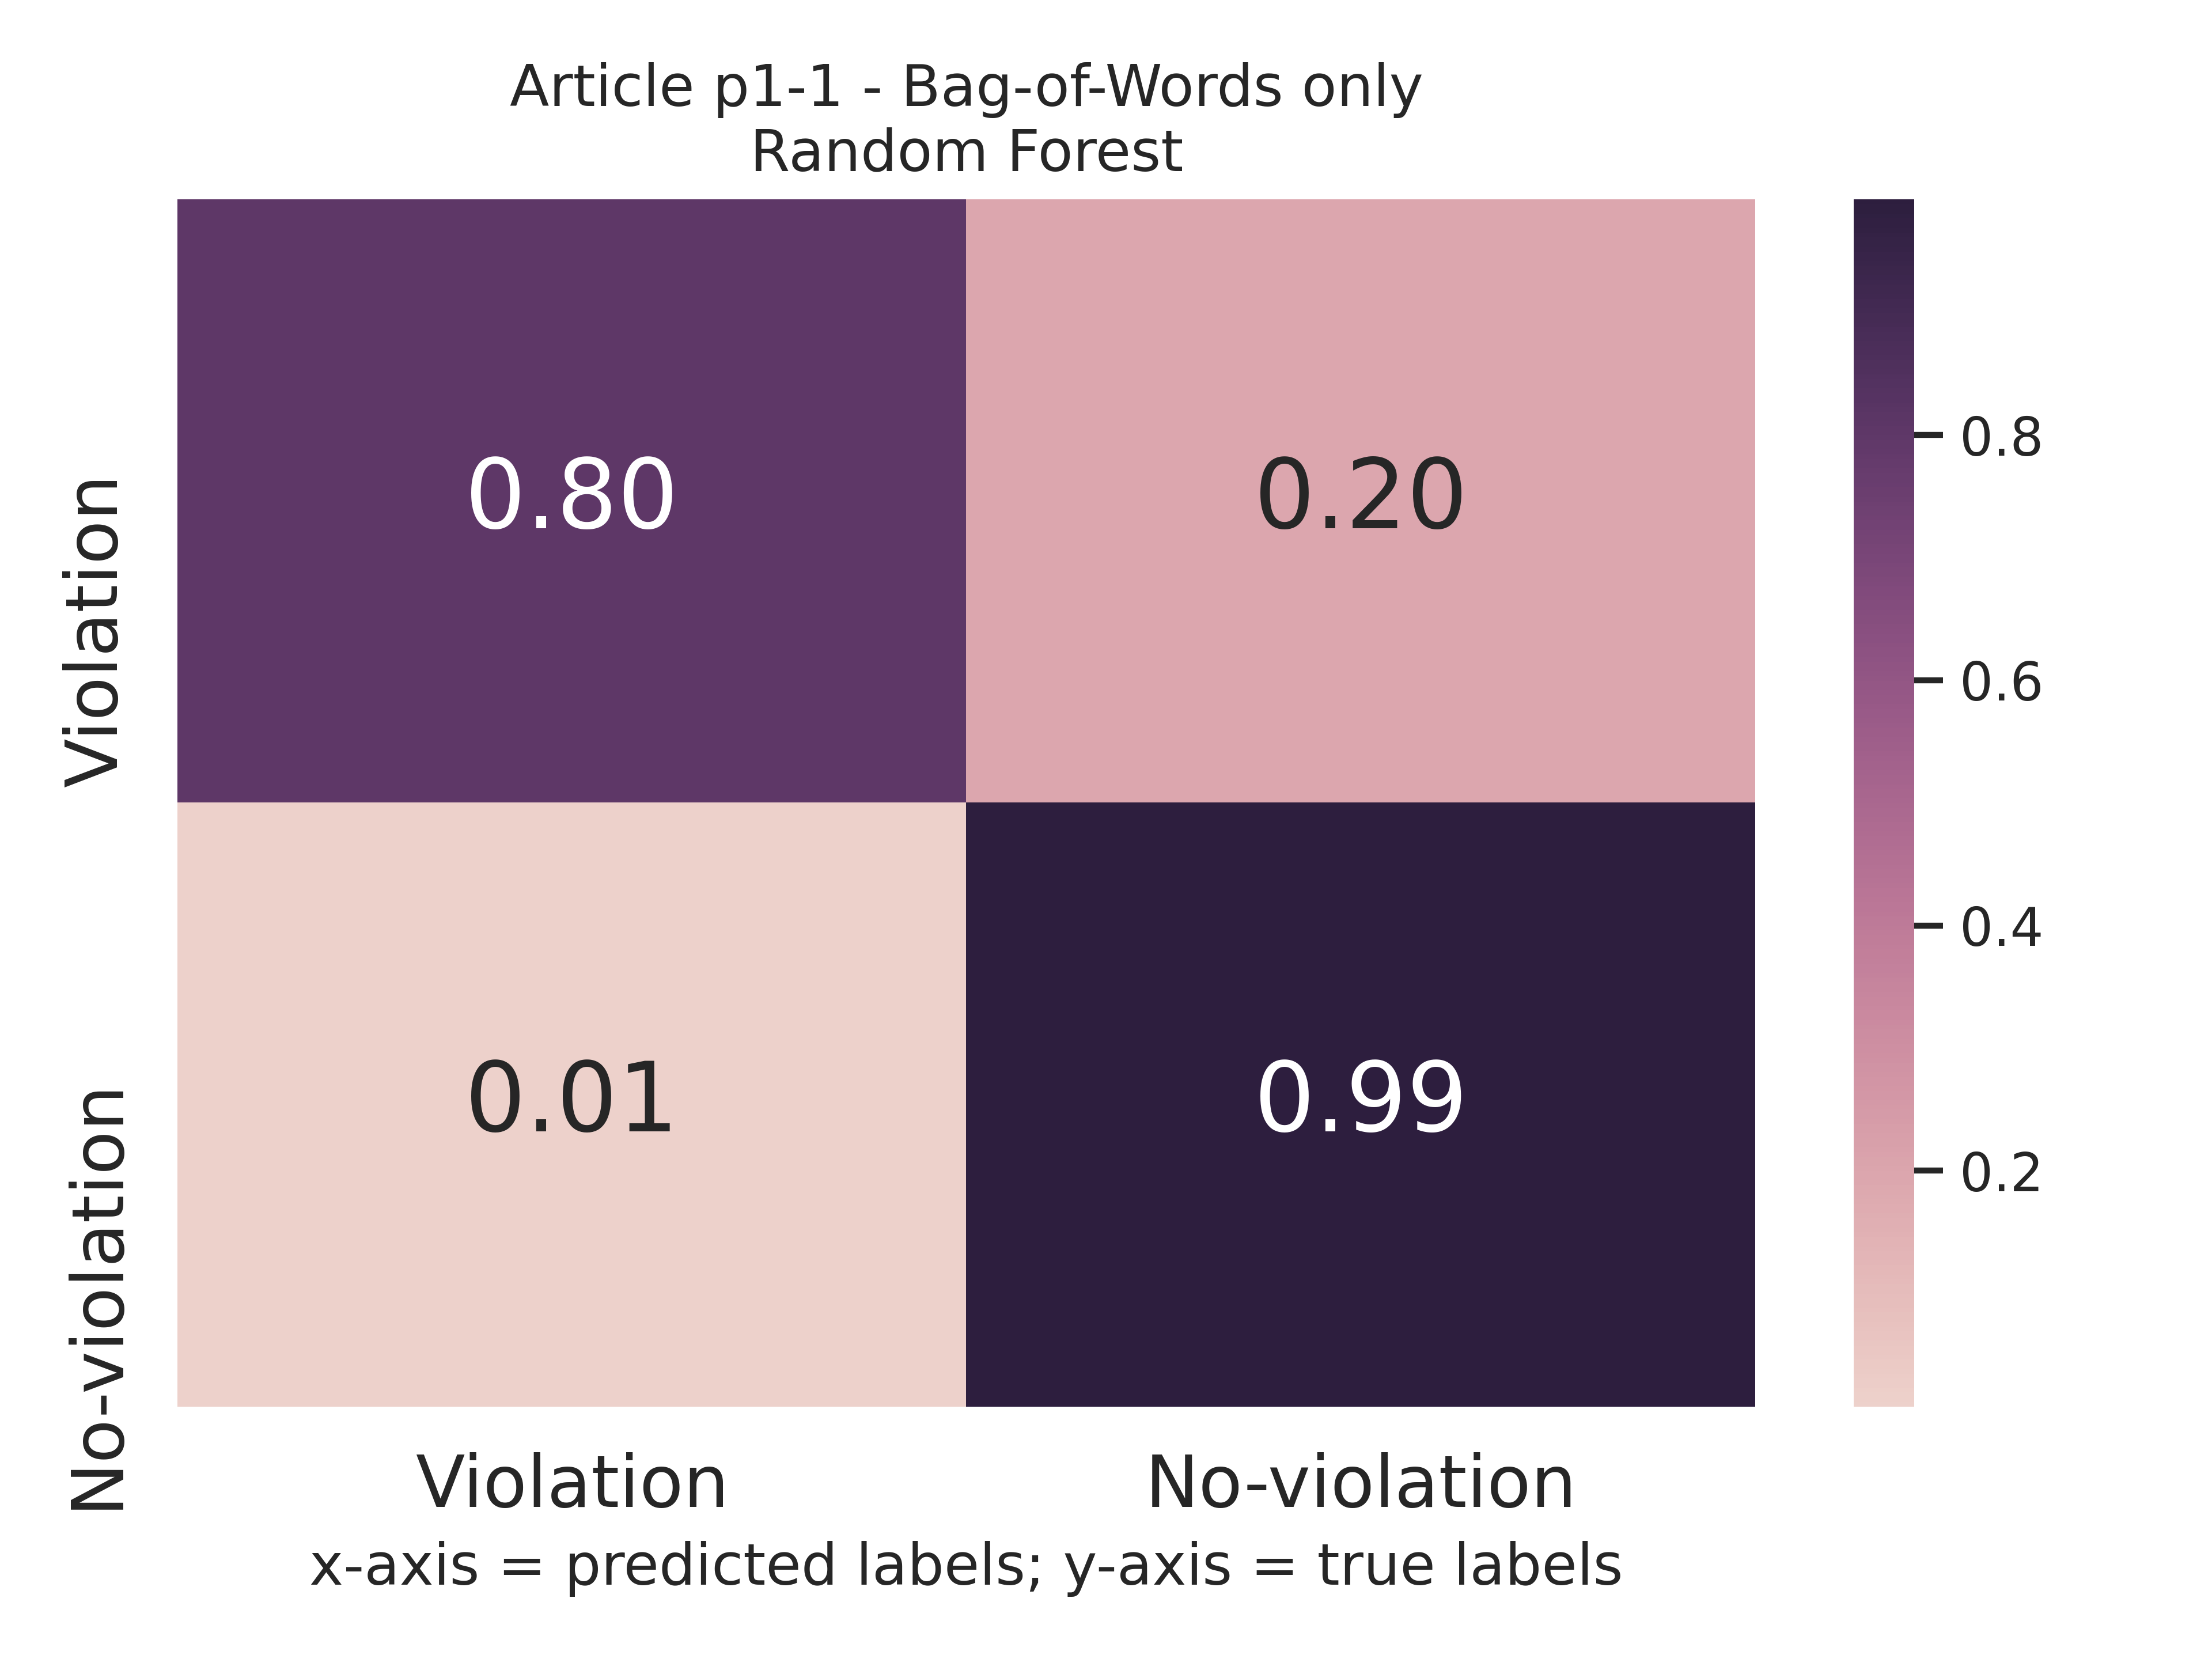
\includegraphics[scale=0.5]{data/analysis/cm/binary_cm_normalized_test_article_p1-1.png}  
\end{figure}

\newpage

\section{Multiclass Classification}

This section presents the results for each method on each article and for all evaluation metrics.
It also reports the best normalized confusion matrices for each article.\\

\noindent
	\begin{tabular}{|l|l|l|l| }
\hline
 &  \multicolumn{3}{c|}{ Accuracy - Multiclass} \\
\cline{2-4} & desc & BoW & both \\ \hline
AdaBoost                & 0.7066 (0.06) & 0.5609 (0.03) & 0.6370 (0.07)\\
BaggingClassifier       & 0.8765 (0.01) & 0.8107 (0.01) & {\bf 0.9219} (0.01)\\
Bernoulli Naive Bayes   & 0.4309 (0.03) & 0.6114 (0.02) & 0.5847 (0.02)\\
Decision Tree           & 0.8607 (0.01) & 0.7523 (0.02) & 0.8927 (0.01)\\
Ensemble Extra Tree     & 0.8519 (0.01) & 0.8159 (0.01) & 0.8451 (0.01)\\
Extra Tree              & 0.6805 (0.03) & 0.6356 (0.02) & 0.6423 (0.02)\\
Gradient Boosting       & 0.8642 (0.01) & 0.8070 (0.02) & 0.9030 (0.01)\\
Linear SVC              & {\bf 0.8814} (0.01) & {\bf 0.8301} (0.02) & 0.9026 (0.01)\\
Multinomial Naive Bayes & 0.6692 (0.02) & 0.6437 (0.02) & 0.6248 (0.02)\\
Neural Net              & 0.8455 (0.01) & 0.8170 (0.02) & 0.8552 (0.01)\\
Random Forest           & 0.8483 (0.01) & 0.8117 (0.01) & 0.8359 (0.01)\\
\hline
\end{tabular}~\\
	\begin{tabular}{|l|l|l|l| }
\hline
 &  \multicolumn{3}{c|}{ Balanced accuracy - Multiclass} \\
\cline{2-4} & desc & BoW & both \\ \hline
AdaBoost                & 0.4451 (0.08) & 0.3890 (0.04) & 0.4162 (0.05)\\
BaggingClassifier       & 0.6665 (0.03) & 0.6838 (0.02) & {\bf 0.8329} (0.03)\\
Bernoulli Naive Bayes   & 0.1111 (0.01) & 0.3501 (0.02) & 0.2794 (0.02)\\
Decision Tree           & 0.6586 (0.03) & 0.6440 (0.03) & 0.8075 (0.03)\\
Ensemble Extra Tree     & 0.5625 (0.03) & {\bf 0.7081} (0.02) & 0.7343 (0.02)\\
Extra Tree              & 0.4681 (0.05) & 0.5009 (0.04) & 0.4838 (0.02)\\
Gradient Boosting       & 0.6251 (0.02) & 0.6161 (0.02) & 0.7268 (0.03)\\
Linear SVC              & {\bf 0.6744} (0.03) & 0.6990 (0.03) & 0.7441 (0.02)\\
Multinomial Naive Bayes & 0.3122 (0.02) & 0.3780 (0.01) & 0.3150 (0.02)\\
Neural Net              & 0.5919 (0.03) & 0.6224 (0.03) & 0.6618 (0.03)\\
Random Forest           & 0.5423 (0.02) & 0.6917 (0.01) & 0.7098 (0.02)\\
\hline
\end{tabular}~\\
	\begin{tabular}{|l|l|l|l| }
\hline
 &  \multicolumn{3}{c|}{ F1 score - Multiclass} \\
\cline{2-4} & desc & BoW & both \\ \hline
AdaBoost                & 0.6709 (0.08) & 0.5485 (0.03) & 0.5824 (0.08)\\
BaggingClassifier       & 0.8684 (0.01) & 0.8064 (0.01) & {\bf 0.9207} (0.01)\\
Bernoulli Naive Bayes   & 0.3324 (0.03) & 0.5757 (0.02) & 0.5362 (0.03)\\
Decision Tree           & 0.8556 (0.01) & 0.7513 (0.02) & 0.8917 (0.01)\\
Ensemble Extra Tree     & 0.8264 (0.01) & 0.8128 (0.01) & 0.8415 (0.01)\\
Extra Tree              & 0.6747 (0.03) & 0.6329 (0.02) & 0.6393 (0.02)\\
Gradient Boosting       & 0.8475 (0.01) & 0.8023 (0.02) & 0.8970 (0.01)\\
Linear SVC              & {\bf 0.8716} (0.01) & {\bf 0.8257} (0.02) & 0.8980 (0.01)\\
Multinomial Naive Bayes & 0.6123 (0.02) & 0.6118 (0.02) & 0.5800 (0.02)\\
Neural Net              & 0.8300 (0.01) & 0.8086 (0.02) & 0.8469 (0.01)\\
Random Forest           & 0.8183 (0.01) & 0.8075 (0.01) & 0.8312 (0.01)\\
\hline
\end{tabular}~\\
	\begin{tabular}{|l|l|l|l| }
\hline
 &  \multicolumn{3}{c|}{ MCC - Multiclass} \\
\cline{2-4} & desc & BoW & both \\ \hline
AdaBoost                & 0.6634 (0.07) & 0.5069 (0.03) & 0.5894 (0.08)\\
BaggingClassifier       & 0.8567 (0.01) & 0.7800 (0.01) & {\bf 0.9096} (0.01)\\
Bernoulli Naive Bayes   & 0.3176 (0.03) & 0.5504 (0.03) & 0.5145 (0.03)\\
Decision Tree           & 0.8385 (0.01) & 0.7131 (0.02) & 0.8758 (0.01)\\
Ensemble Extra Tree     & 0.8280 (0.01) & 0.7867 (0.02) & 0.8205 (0.01)\\
Extra Tree              & 0.6294 (0.03) & 0.5779 (0.02) & 0.5853 (0.03)\\
Gradient Boosting       & 0.8422 (0.01) & 0.7758 (0.02) & 0.8877 (0.01)\\
Linear SVC              & {\bf 0.8622} (0.01) & {\bf 0.8027} (0.02) & 0.8870 (0.02)\\
Multinomial Naive Bayes & 0.6088 (0.02) & 0.5896 (0.02) & 0.5651 (0.02)\\
Neural Net              & 0.8205 (0.01) & 0.7873 (0.03) & 0.8320 (0.01)\\
Random Forest           & 0.8238 (0.01) & 0.7817 (0.01) & 0.8099 (0.01)\\
\hline
\end{tabular}~\\
	\begin{tabular}{|l|l|l|l| }
\hline
 &  \multicolumn{3}{c|}{ Precision - Multiclass} \\
\cline{2-4} & desc & BoW & both \\ \hline
AdaBoost                & 0.6789 (0.08) & 0.5898 (0.04) & 0.6312 (0.06)\\
BaggingClassifier       & 0.8695 (0.01) & 0.8123 (0.01) & {\bf 0.9250} (0.01)\\
Bernoulli Naive Bayes   & 0.3845 (0.05) & 0.6065 (0.03) & 0.5650 (0.02)\\
Decision Tree           & 0.8585 (0.01) & 0.7561 (0.02) & 0.8954 (0.01)\\
Ensemble Extra Tree     & 0.8344 (0.02) & 0.8219 (0.01) & 0.8487 (0.01)\\
Extra Tree              & 0.6763 (0.03) & 0.6370 (0.02) & 0.6417 (0.02)\\
Gradient Boosting       & 0.8464 (0.01) & 0.8039 (0.02) & 0.8971 (0.01)\\
Linear SVC              & {\bf 0.8739} (0.01) & {\bf 0.8321} (0.02) & 0.9023 (0.01)\\
Multinomial Naive Bayes & 0.6145 (0.03) & 0.6470 (0.02) & 0.6102 (0.02)\\
Neural Net              & 0.8328 (0.01) & 0.8147 (0.02) & 0.8499 (0.01)\\
Random Forest           & 0.8301 (0.02) & 0.8185 (0.01) & 0.8404 (0.01)\\
\hline
\end{tabular}~\\
	\begin{tabular}{|l|l|l|l| }
\hline
 &  \multicolumn{3}{c|}{ Recall - Multiclass} \\
\cline{2-4} & desc & BoW & both \\ \hline
AdaBoost                & 0.7066 (0.06) & 0.5609 (0.03) & 0.6370 (0.07)\\
BaggingClassifier       & 0.8765 (0.01) & 0.8107 (0.01) & {\bf 0.9219} (0.01)\\
Bernoulli Naive Bayes   & 0.4309 (0.03) & 0.6114 (0.02) & 0.5847 (0.02)\\
Decision Tree           & 0.8607 (0.01) & 0.7523 (0.02) & 0.8927 (0.01)\\
Ensemble Extra Tree     & 0.8519 (0.01) & 0.8159 (0.01) & 0.8451 (0.01)\\
Extra Tree              & 0.6805 (0.03) & 0.6356 (0.02) & 0.6423 (0.02)\\
Gradient Boosting       & 0.8642 (0.01) & 0.8070 (0.02) & 0.9030 (0.01)\\
Linear SVC              & {\bf 0.8814} (0.01) & {\bf 0.8301} (0.02) & 0.9026 (0.01)\\
Multinomial Naive Bayes & 0.6692 (0.02) & 0.6437 (0.02) & 0.6248 (0.02)\\
Neural Net              & 0.8455 (0.01) & 0.8170 (0.02) & 0.8552 (0.01)\\
Random Forest           & 0.8483 (0.01) & 0.8117 (0.01) & 0.8359 (0.01)\\
\hline
\end{tabular}~\\

~\\\newpage
\begin{figure}[!htb]
    \centering
    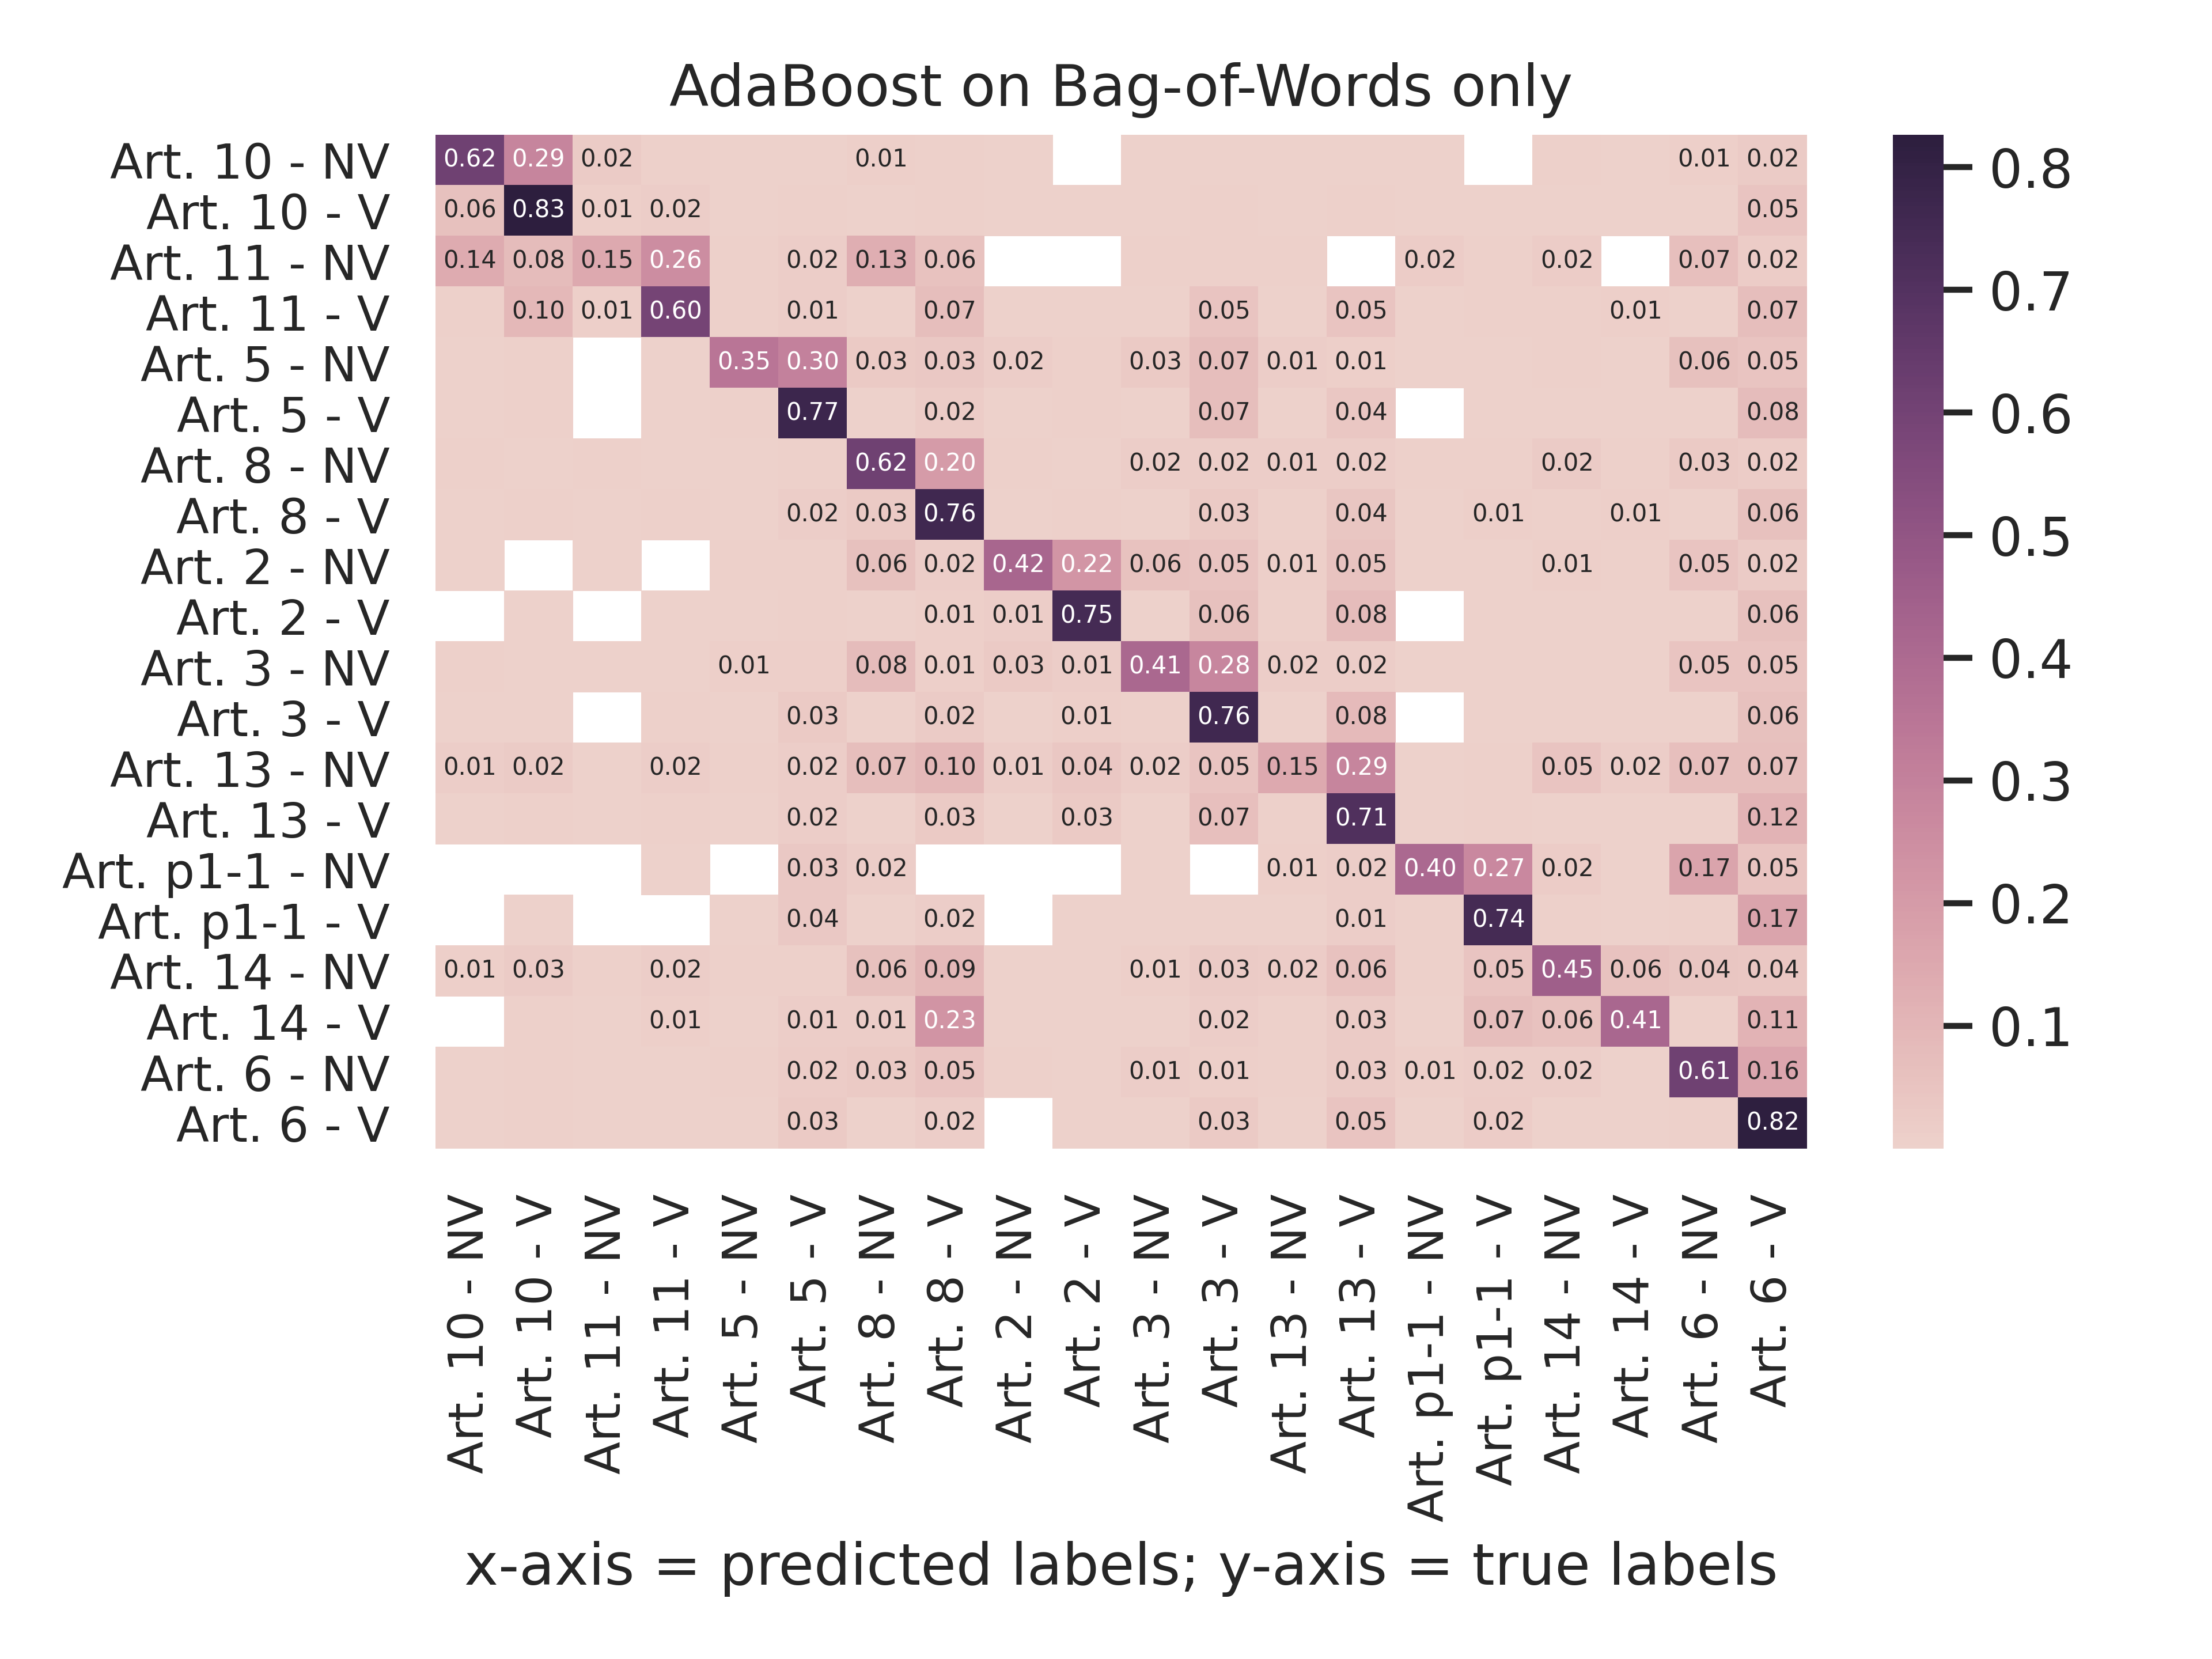
\includegraphics[scale=0.7]{data/analysis/cm/multiclass_cm_test_adaboost_bag-of-words_only.png}  
\end{figure}
\begin{figure}[!htb]
    \centering
    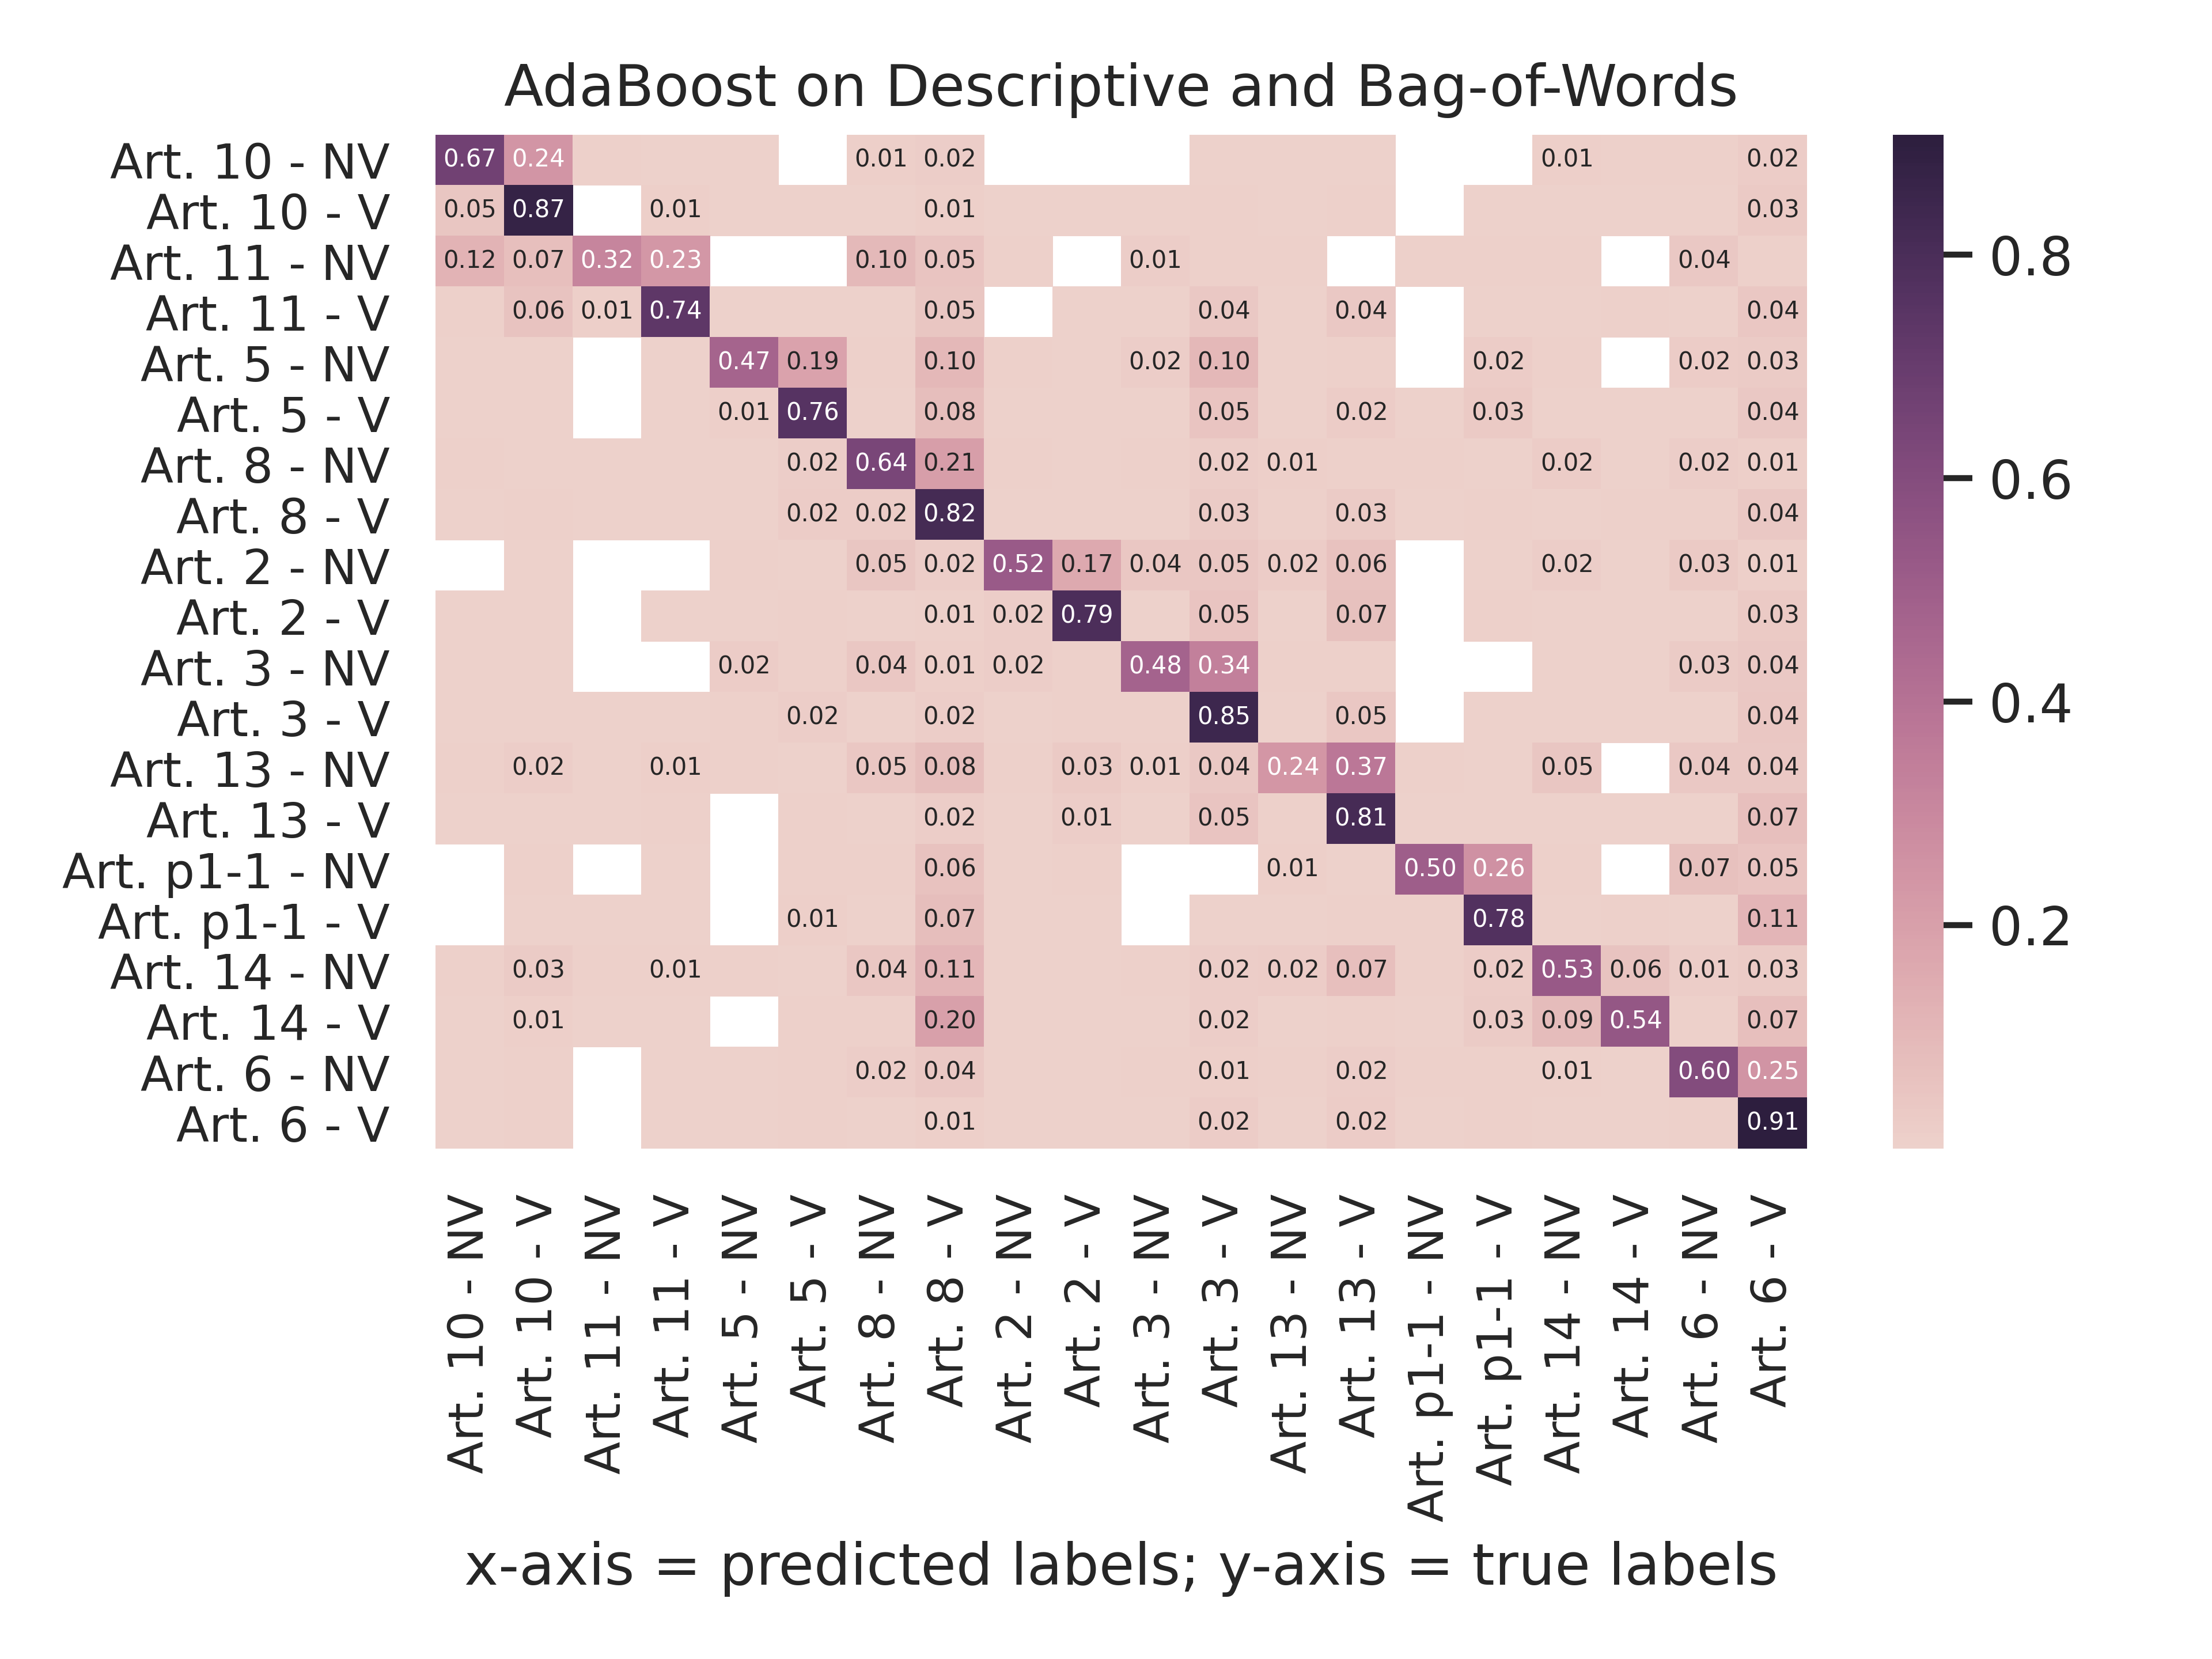
\includegraphics[scale=0.7]{data/analysis/cm/multiclass_cm_test_adaboost_descriptive_and_bag-of-words.png}  
\end{figure}
\begin{figure}[!htb]
    \centering
    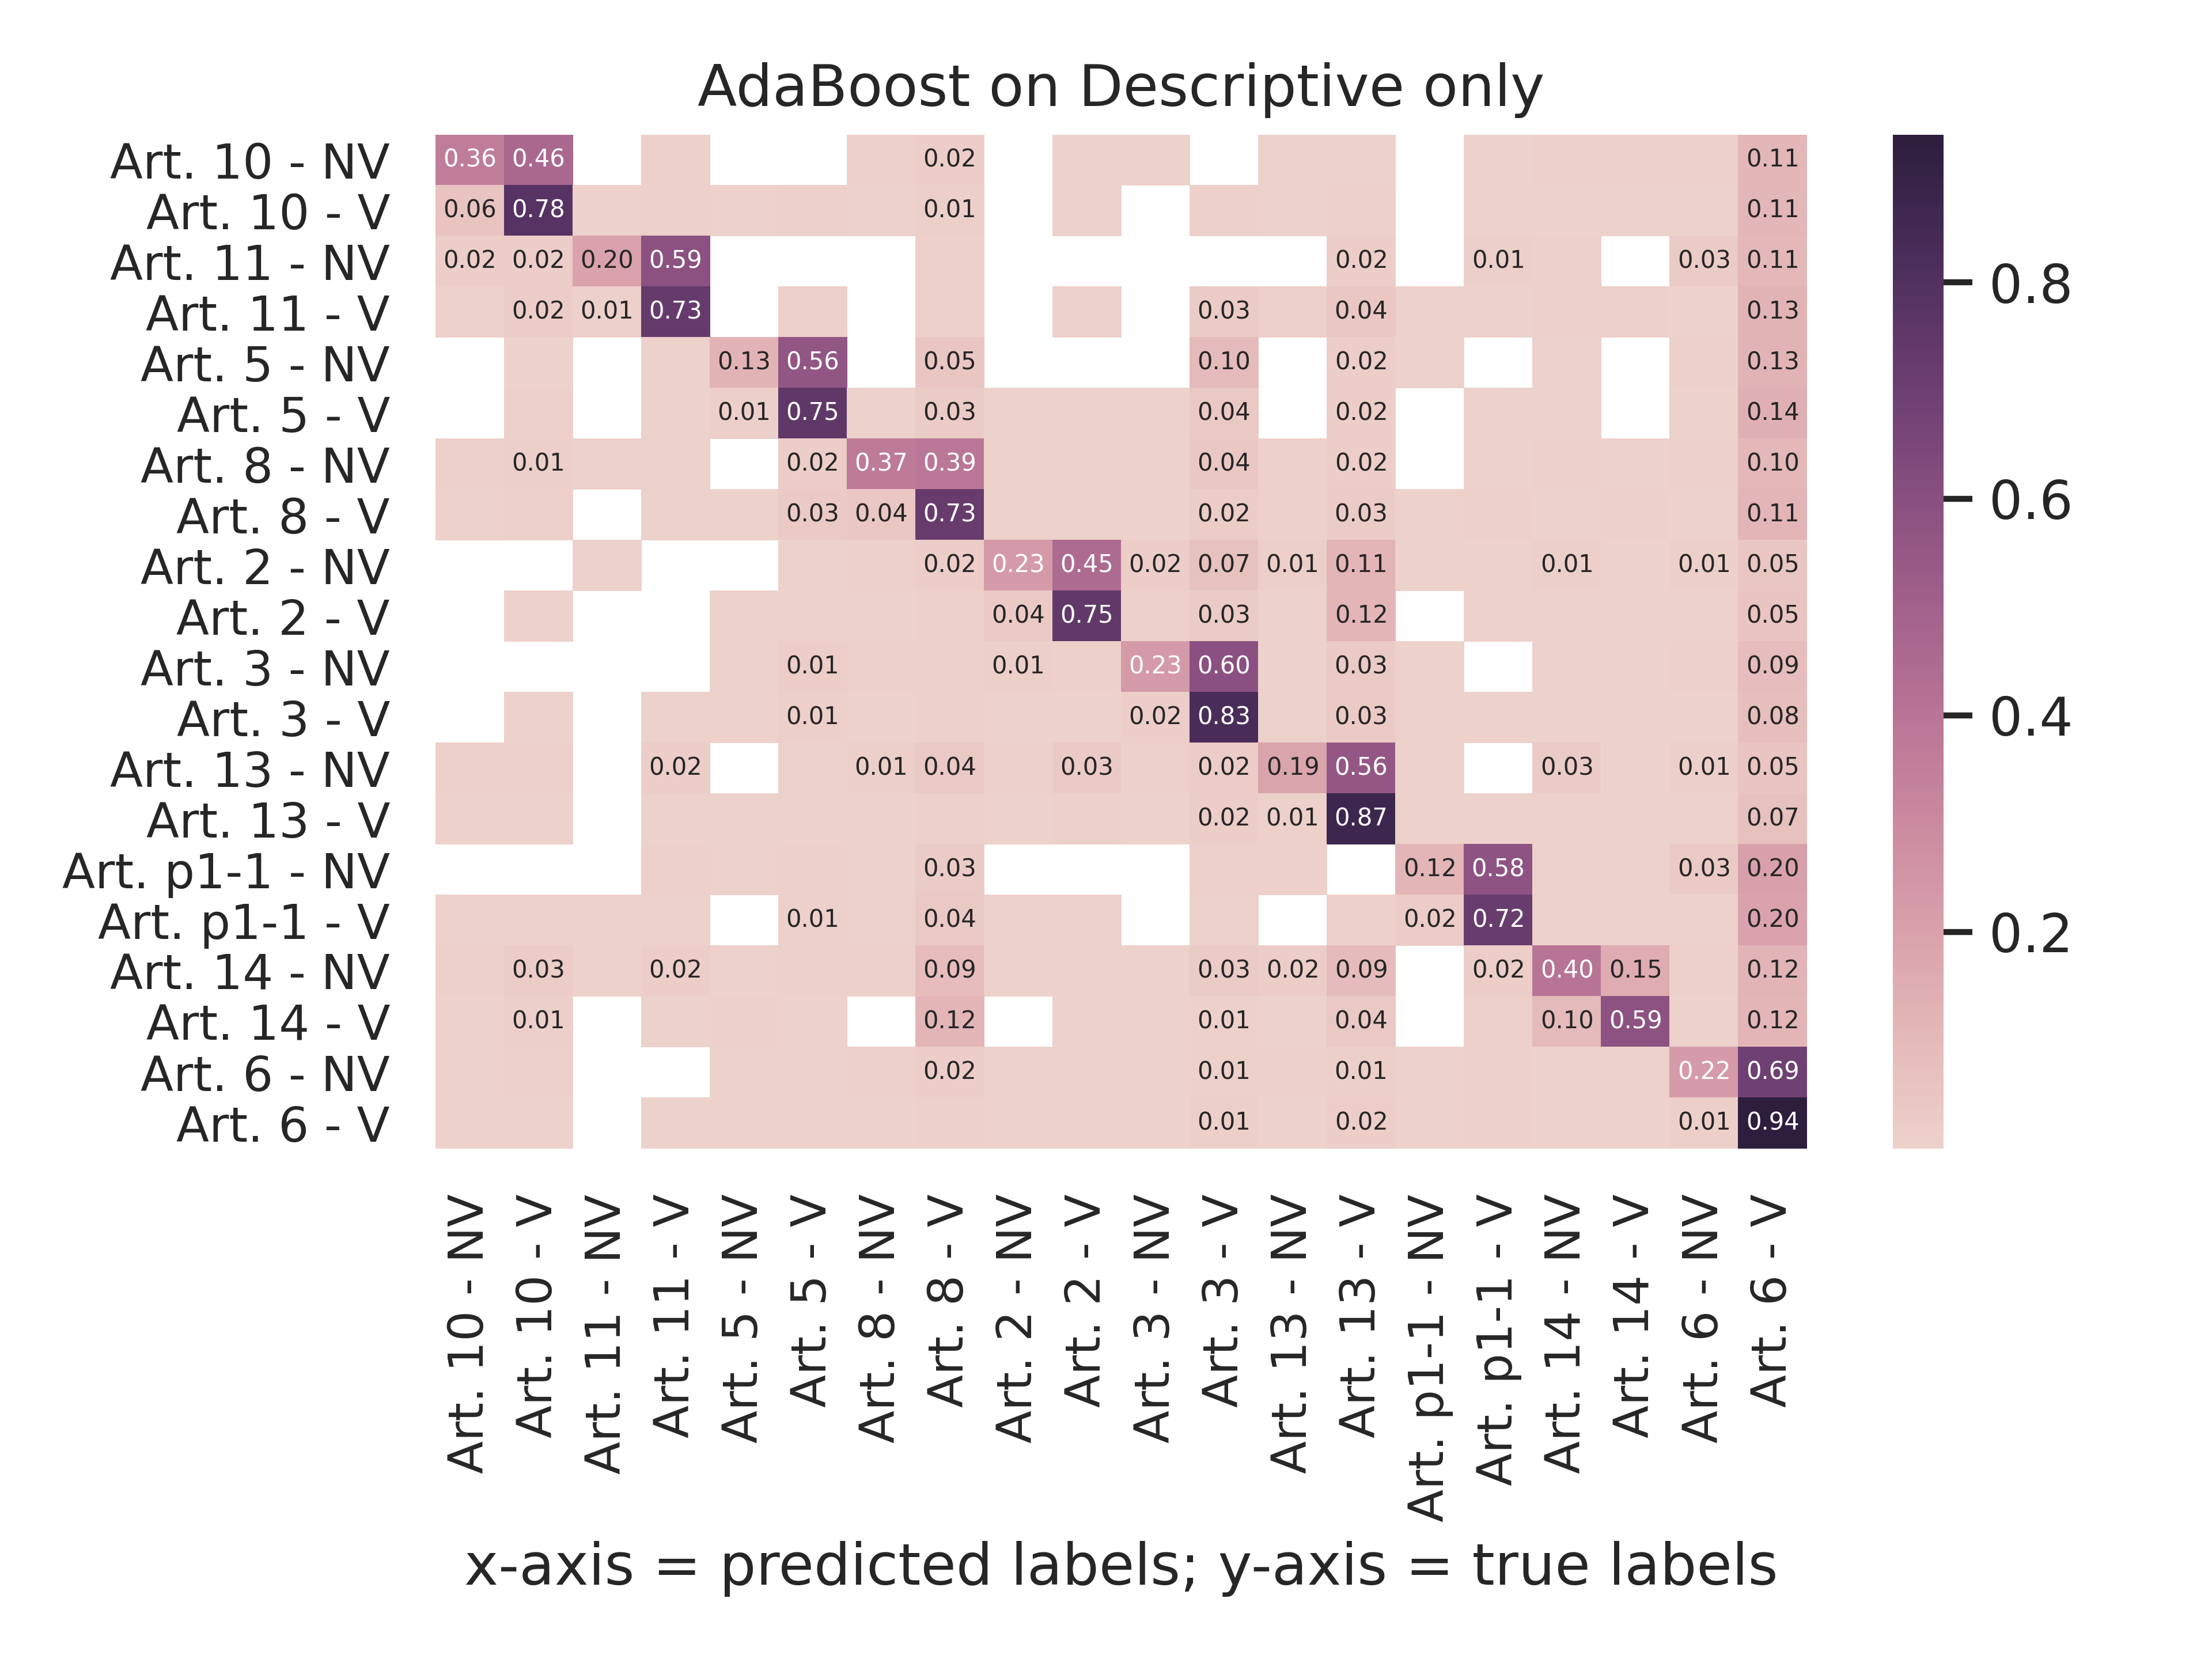
\includegraphics[scale=0.7]{data/analysis/cm/multiclass_cm_test_adaboost_descriptive_only.png}  
\end{figure}
\begin{figure}[!htb]
    \centering
    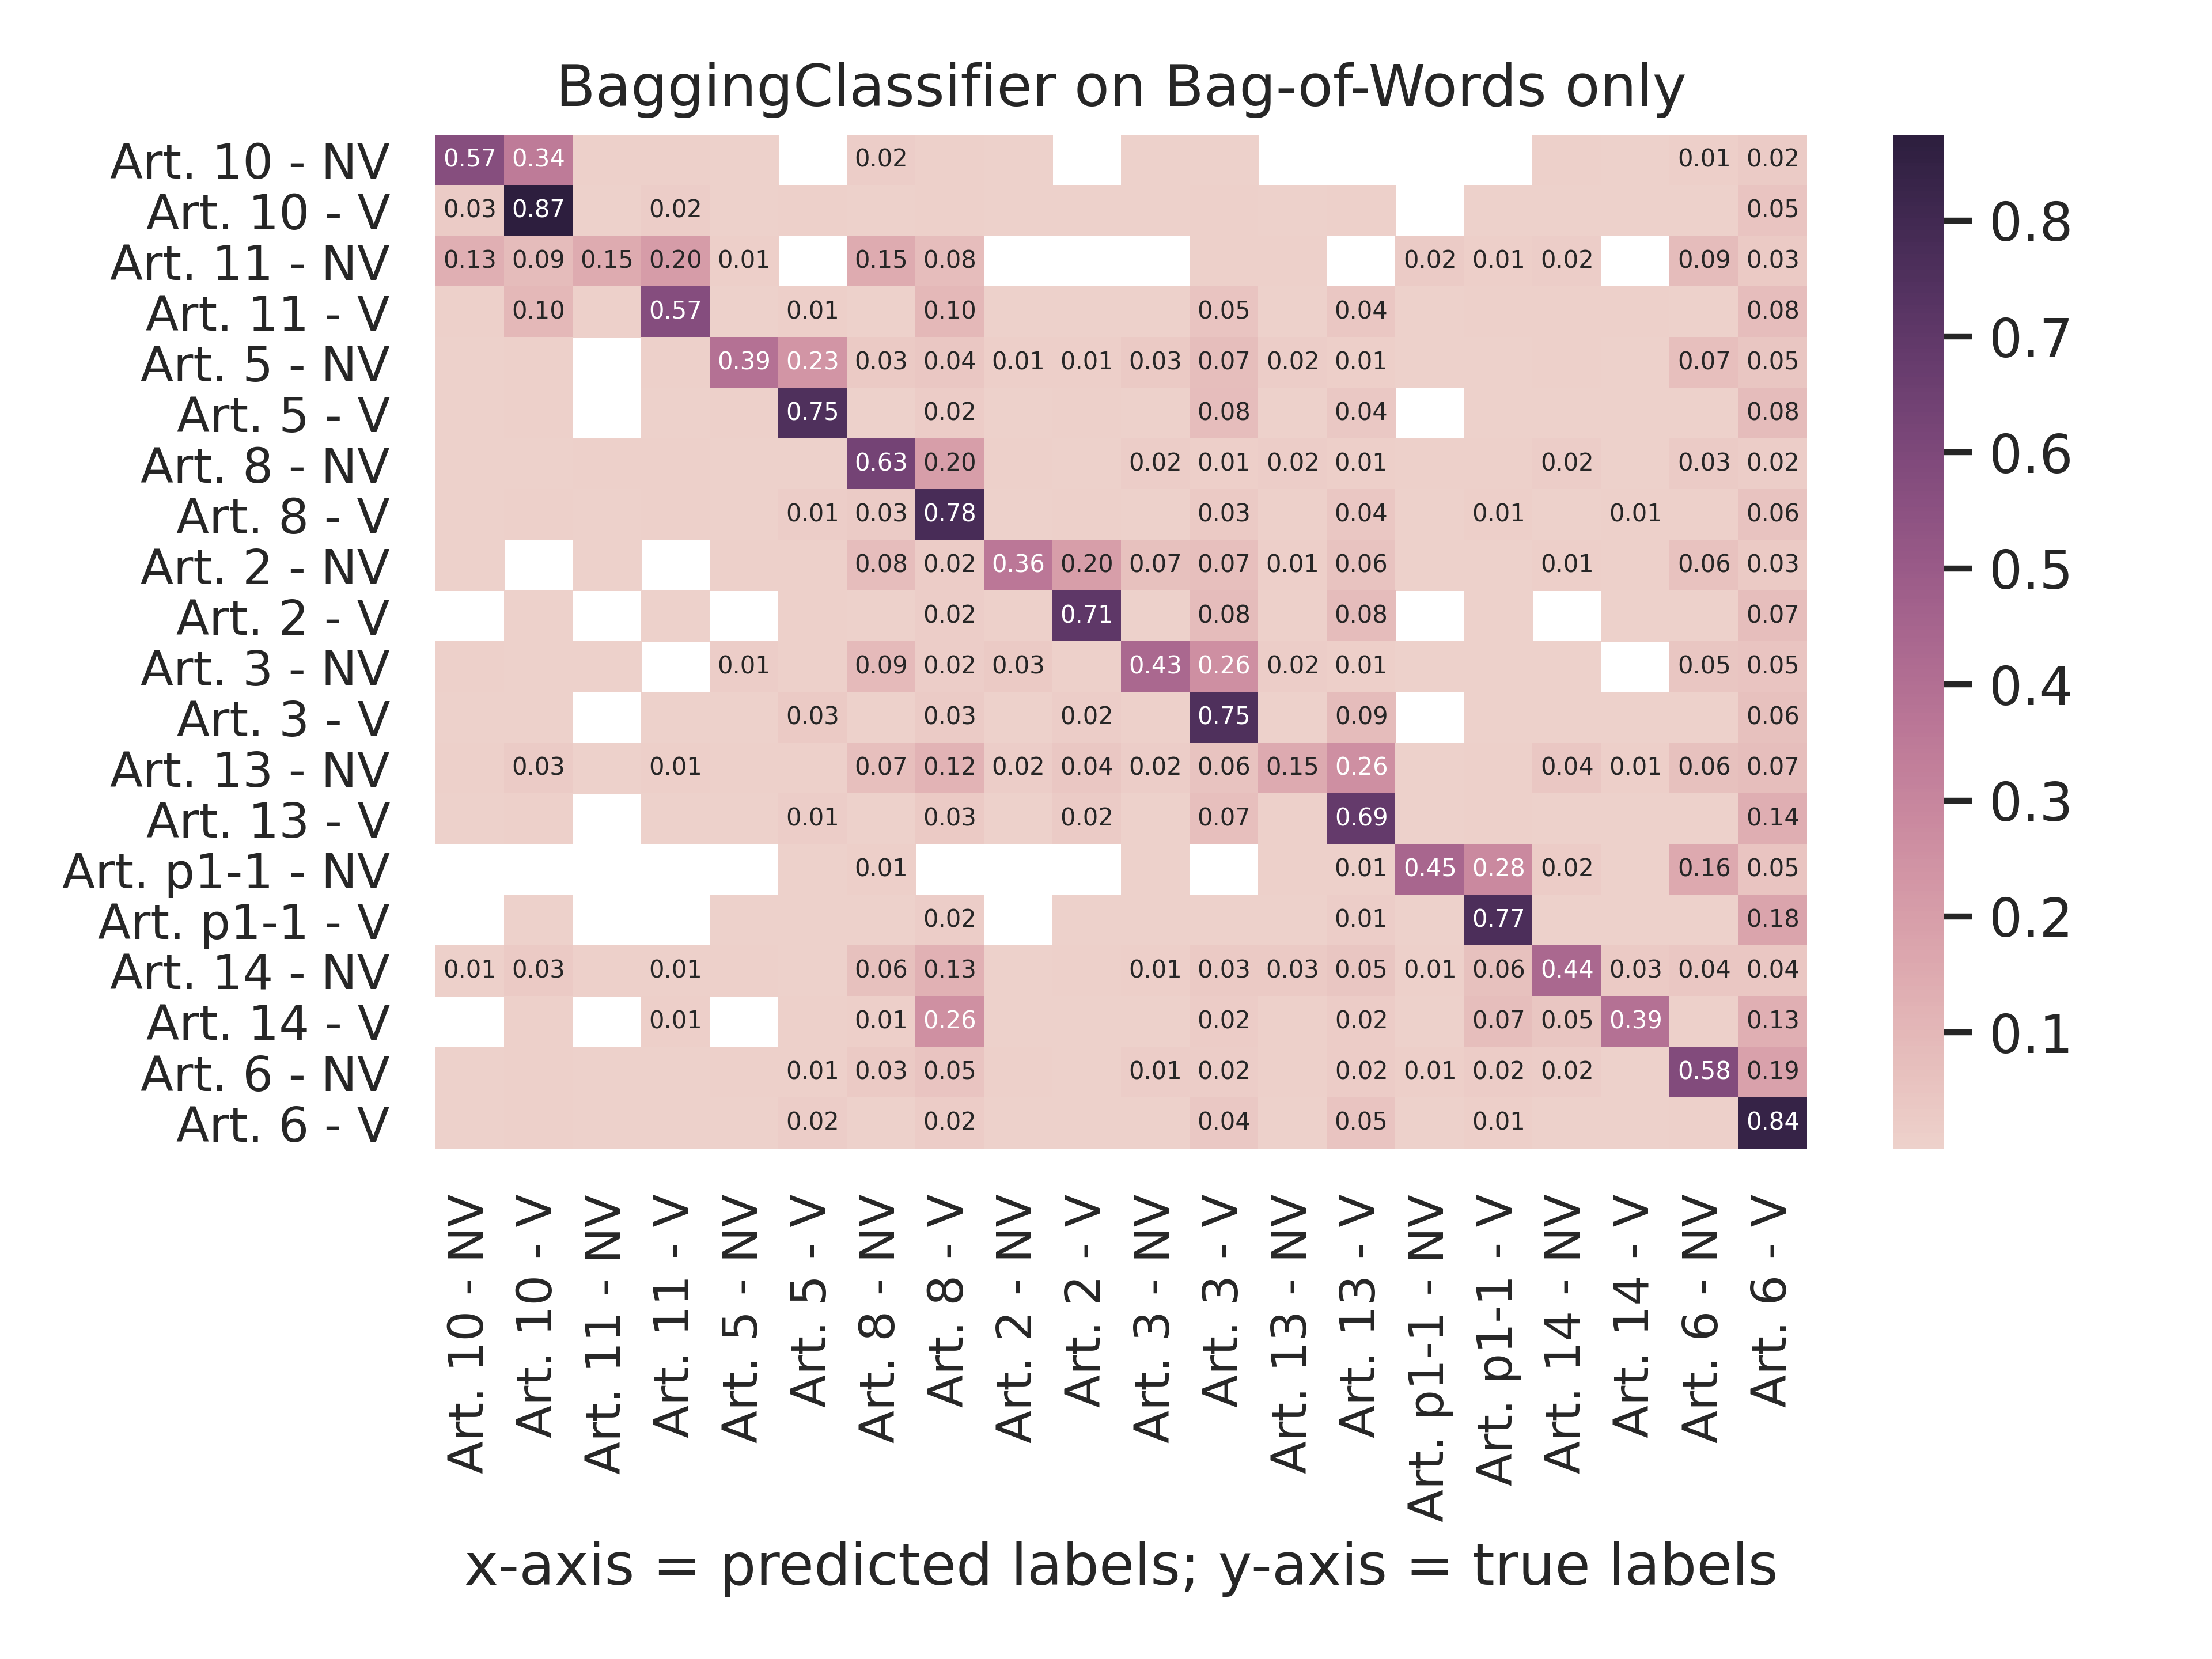
\includegraphics[scale=0.7]{data/analysis/cm/multiclass_cm_test_baggingclassifier_bag-of-words_only.png}  
\end{figure}
\begin{figure}[!htb]
    \centering
    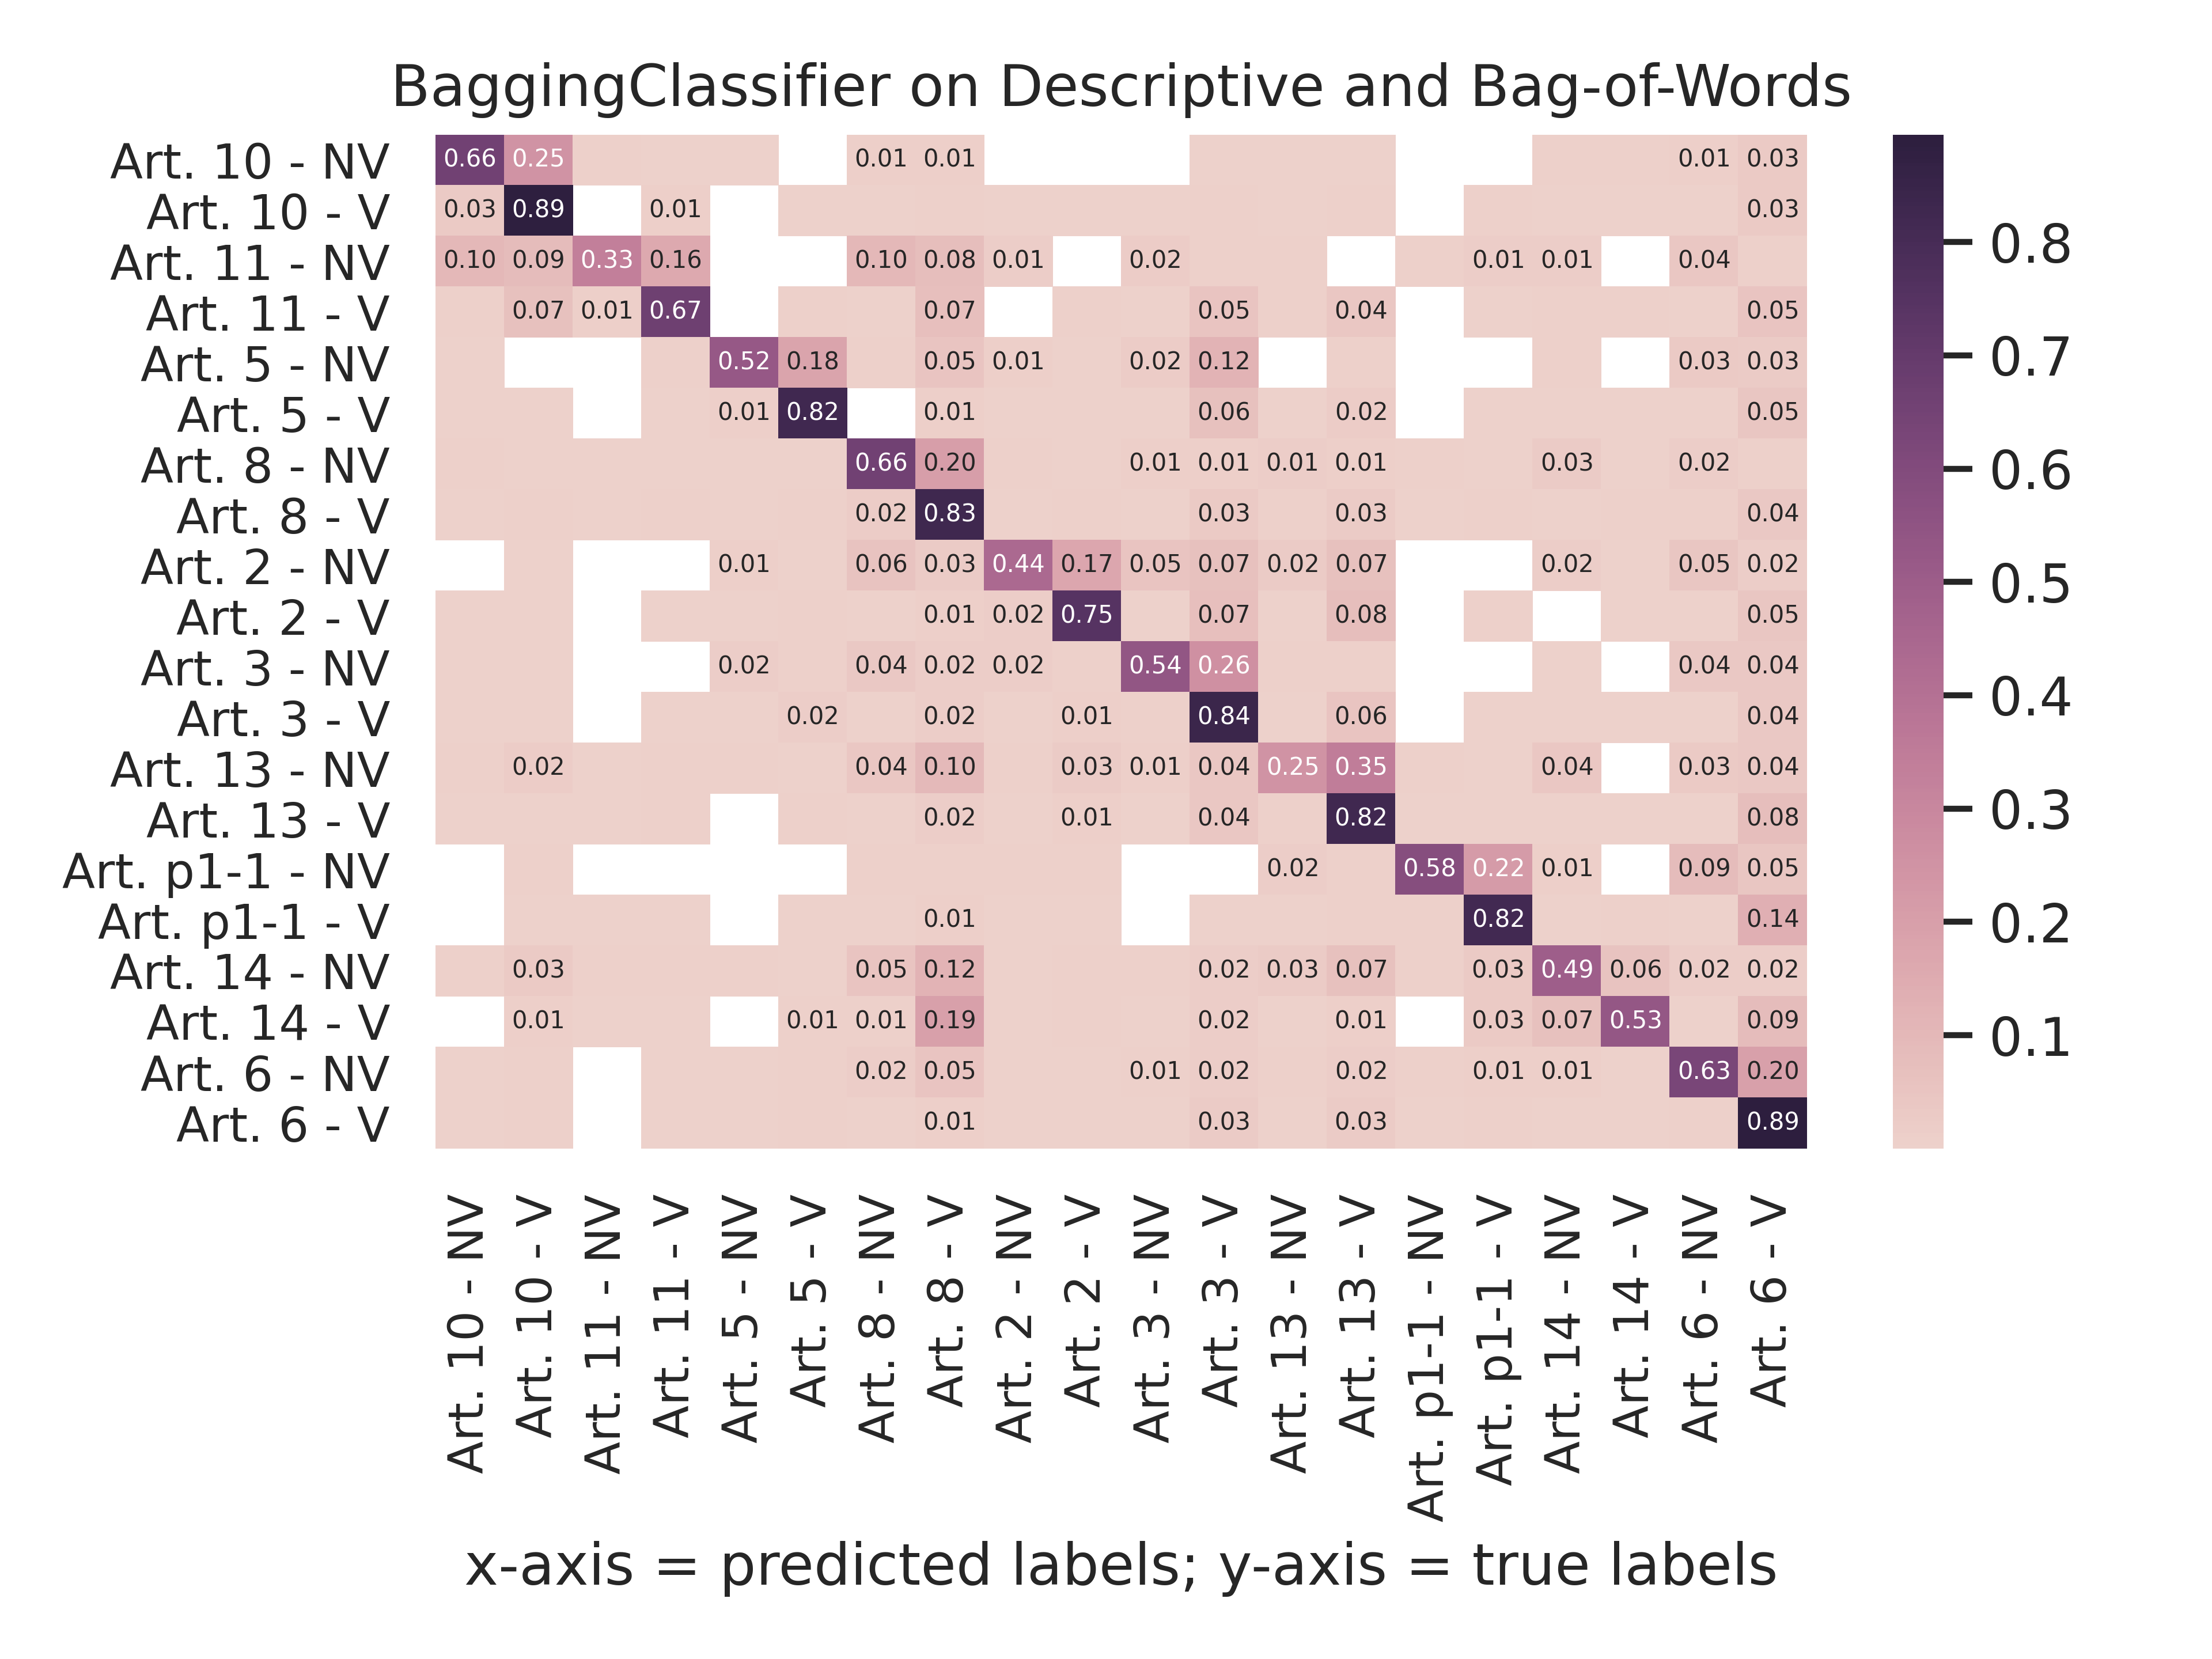
\includegraphics[scale=0.7]{data/analysis/cm/multiclass_cm_test_baggingclassifier_descriptive_and_bag-of-words.png}  
\end{figure}
\begin{figure}[!htb]
    \centering
    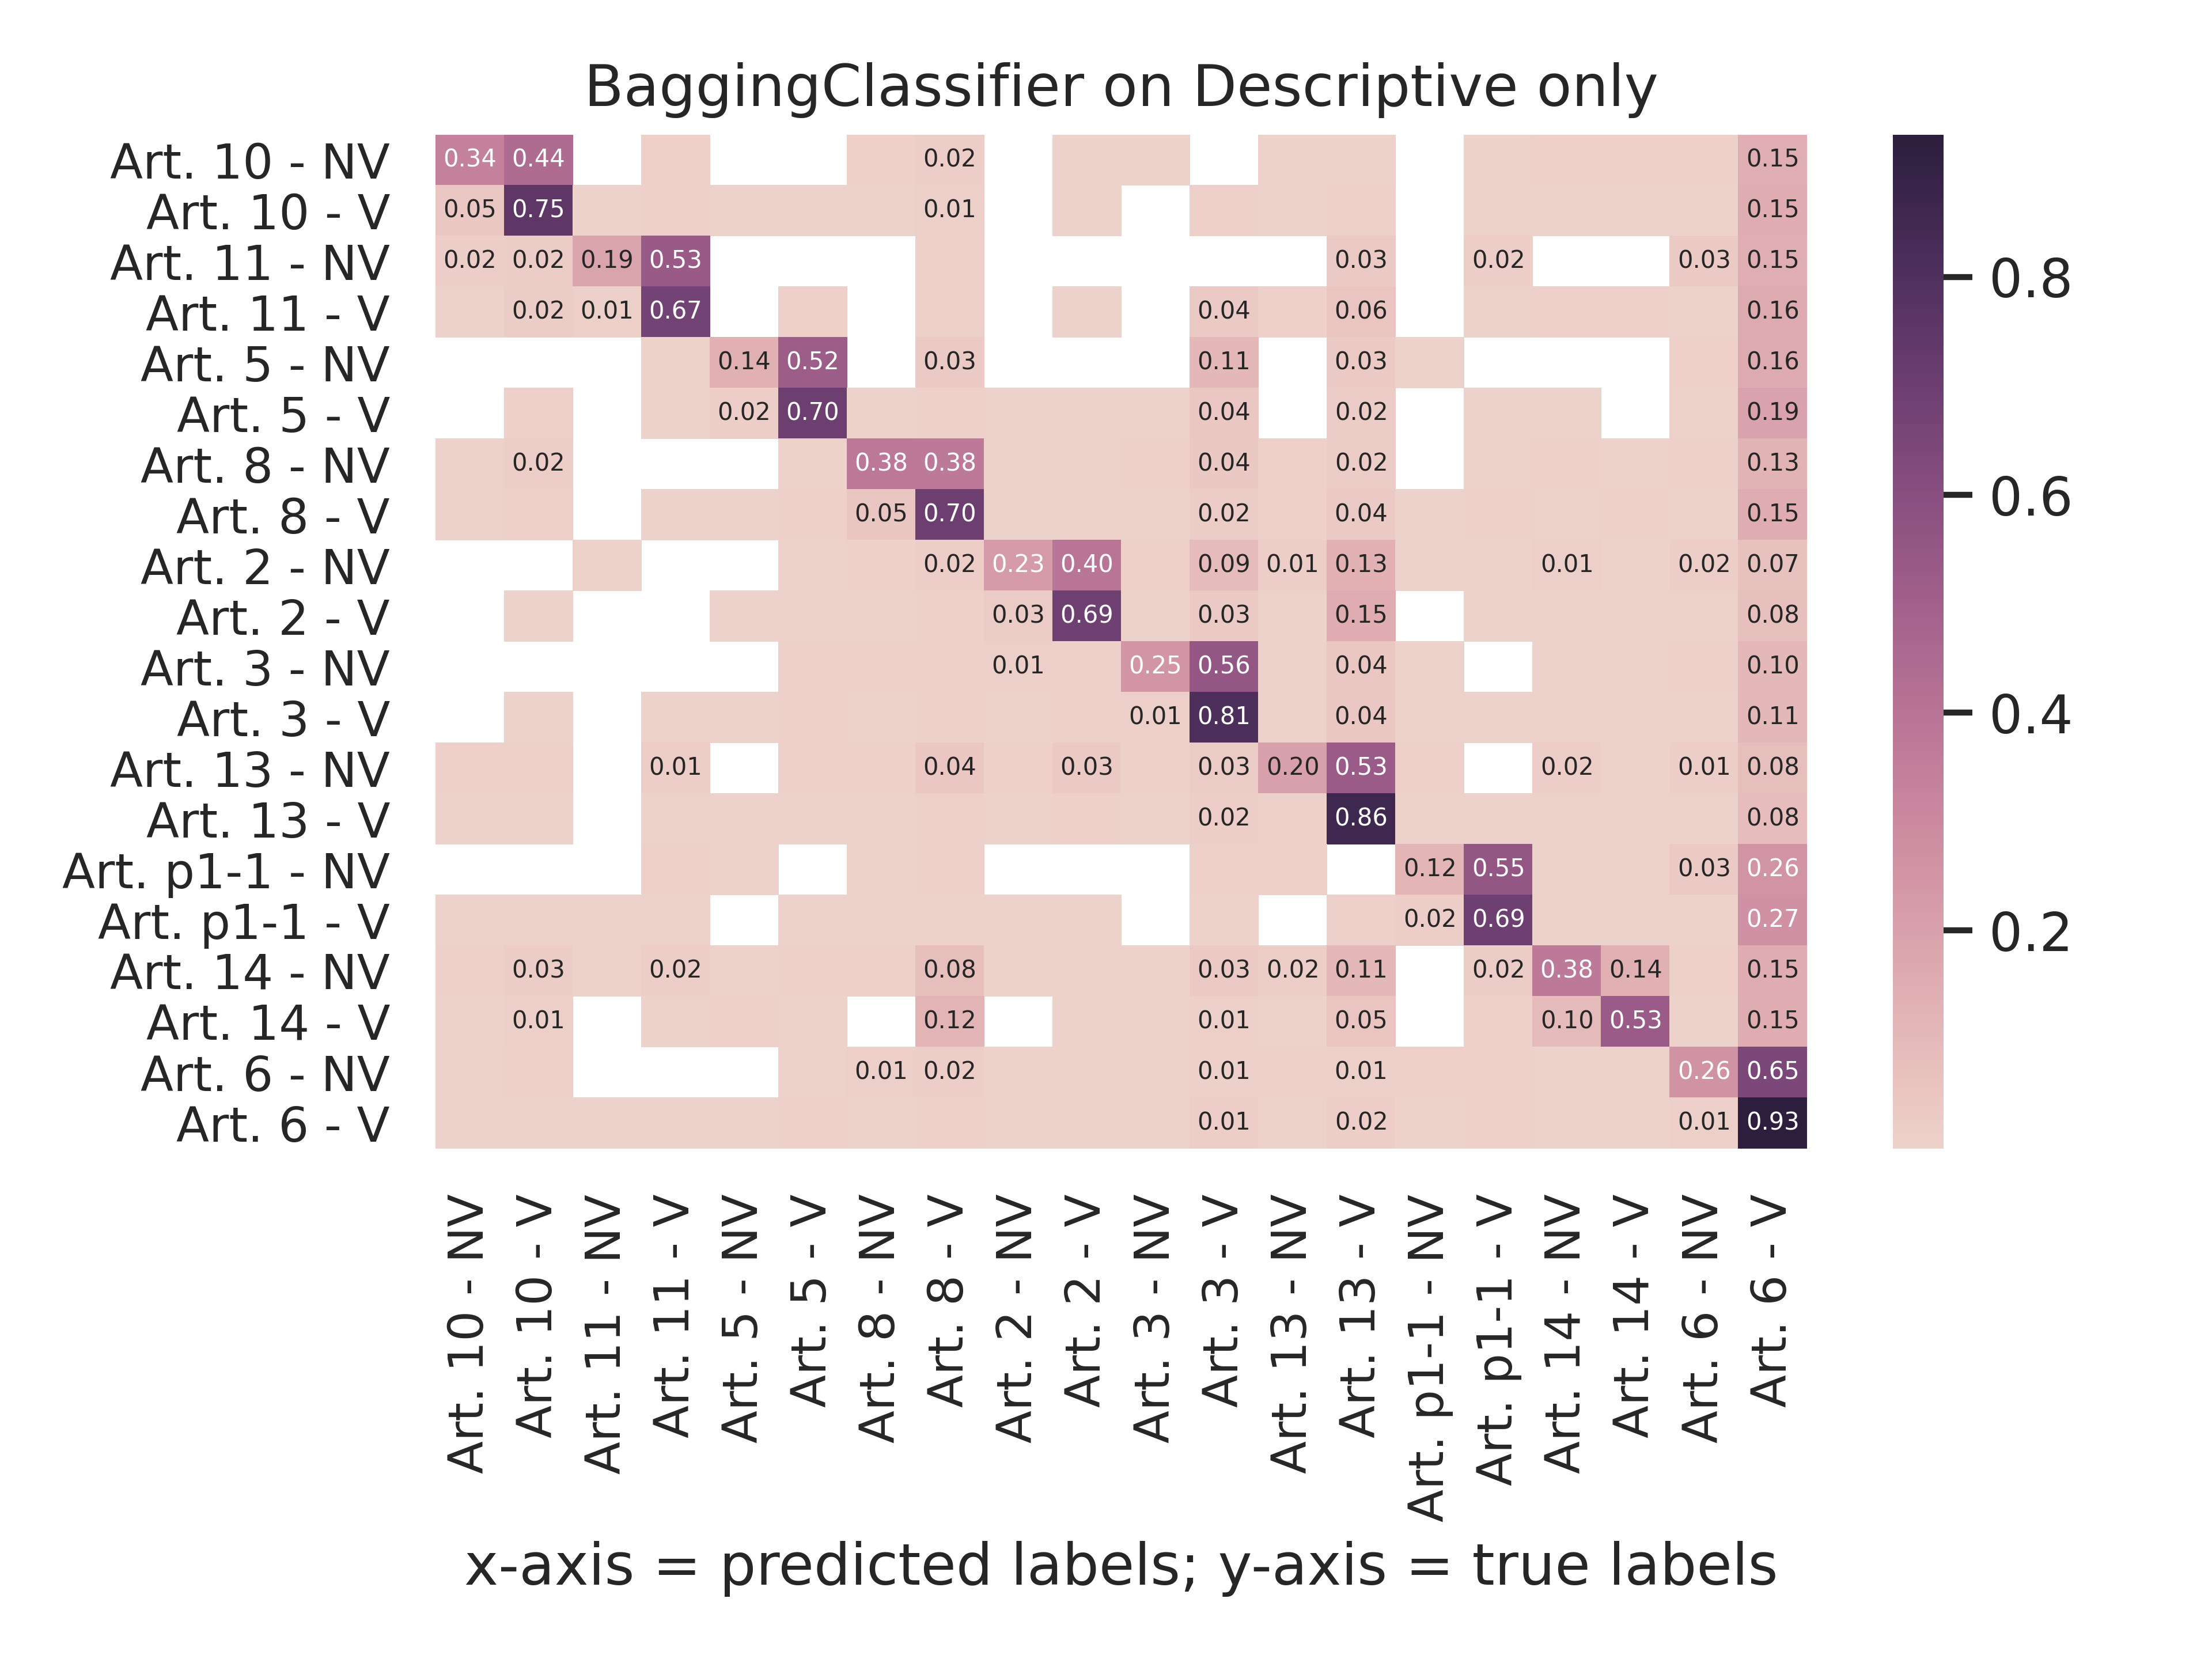
\includegraphics[scale=0.7]{data/analysis/cm/multiclass_cm_test_baggingclassifier_descriptive_only.png}  
\end{figure}
\begin{figure}[!htb]
    \centering
    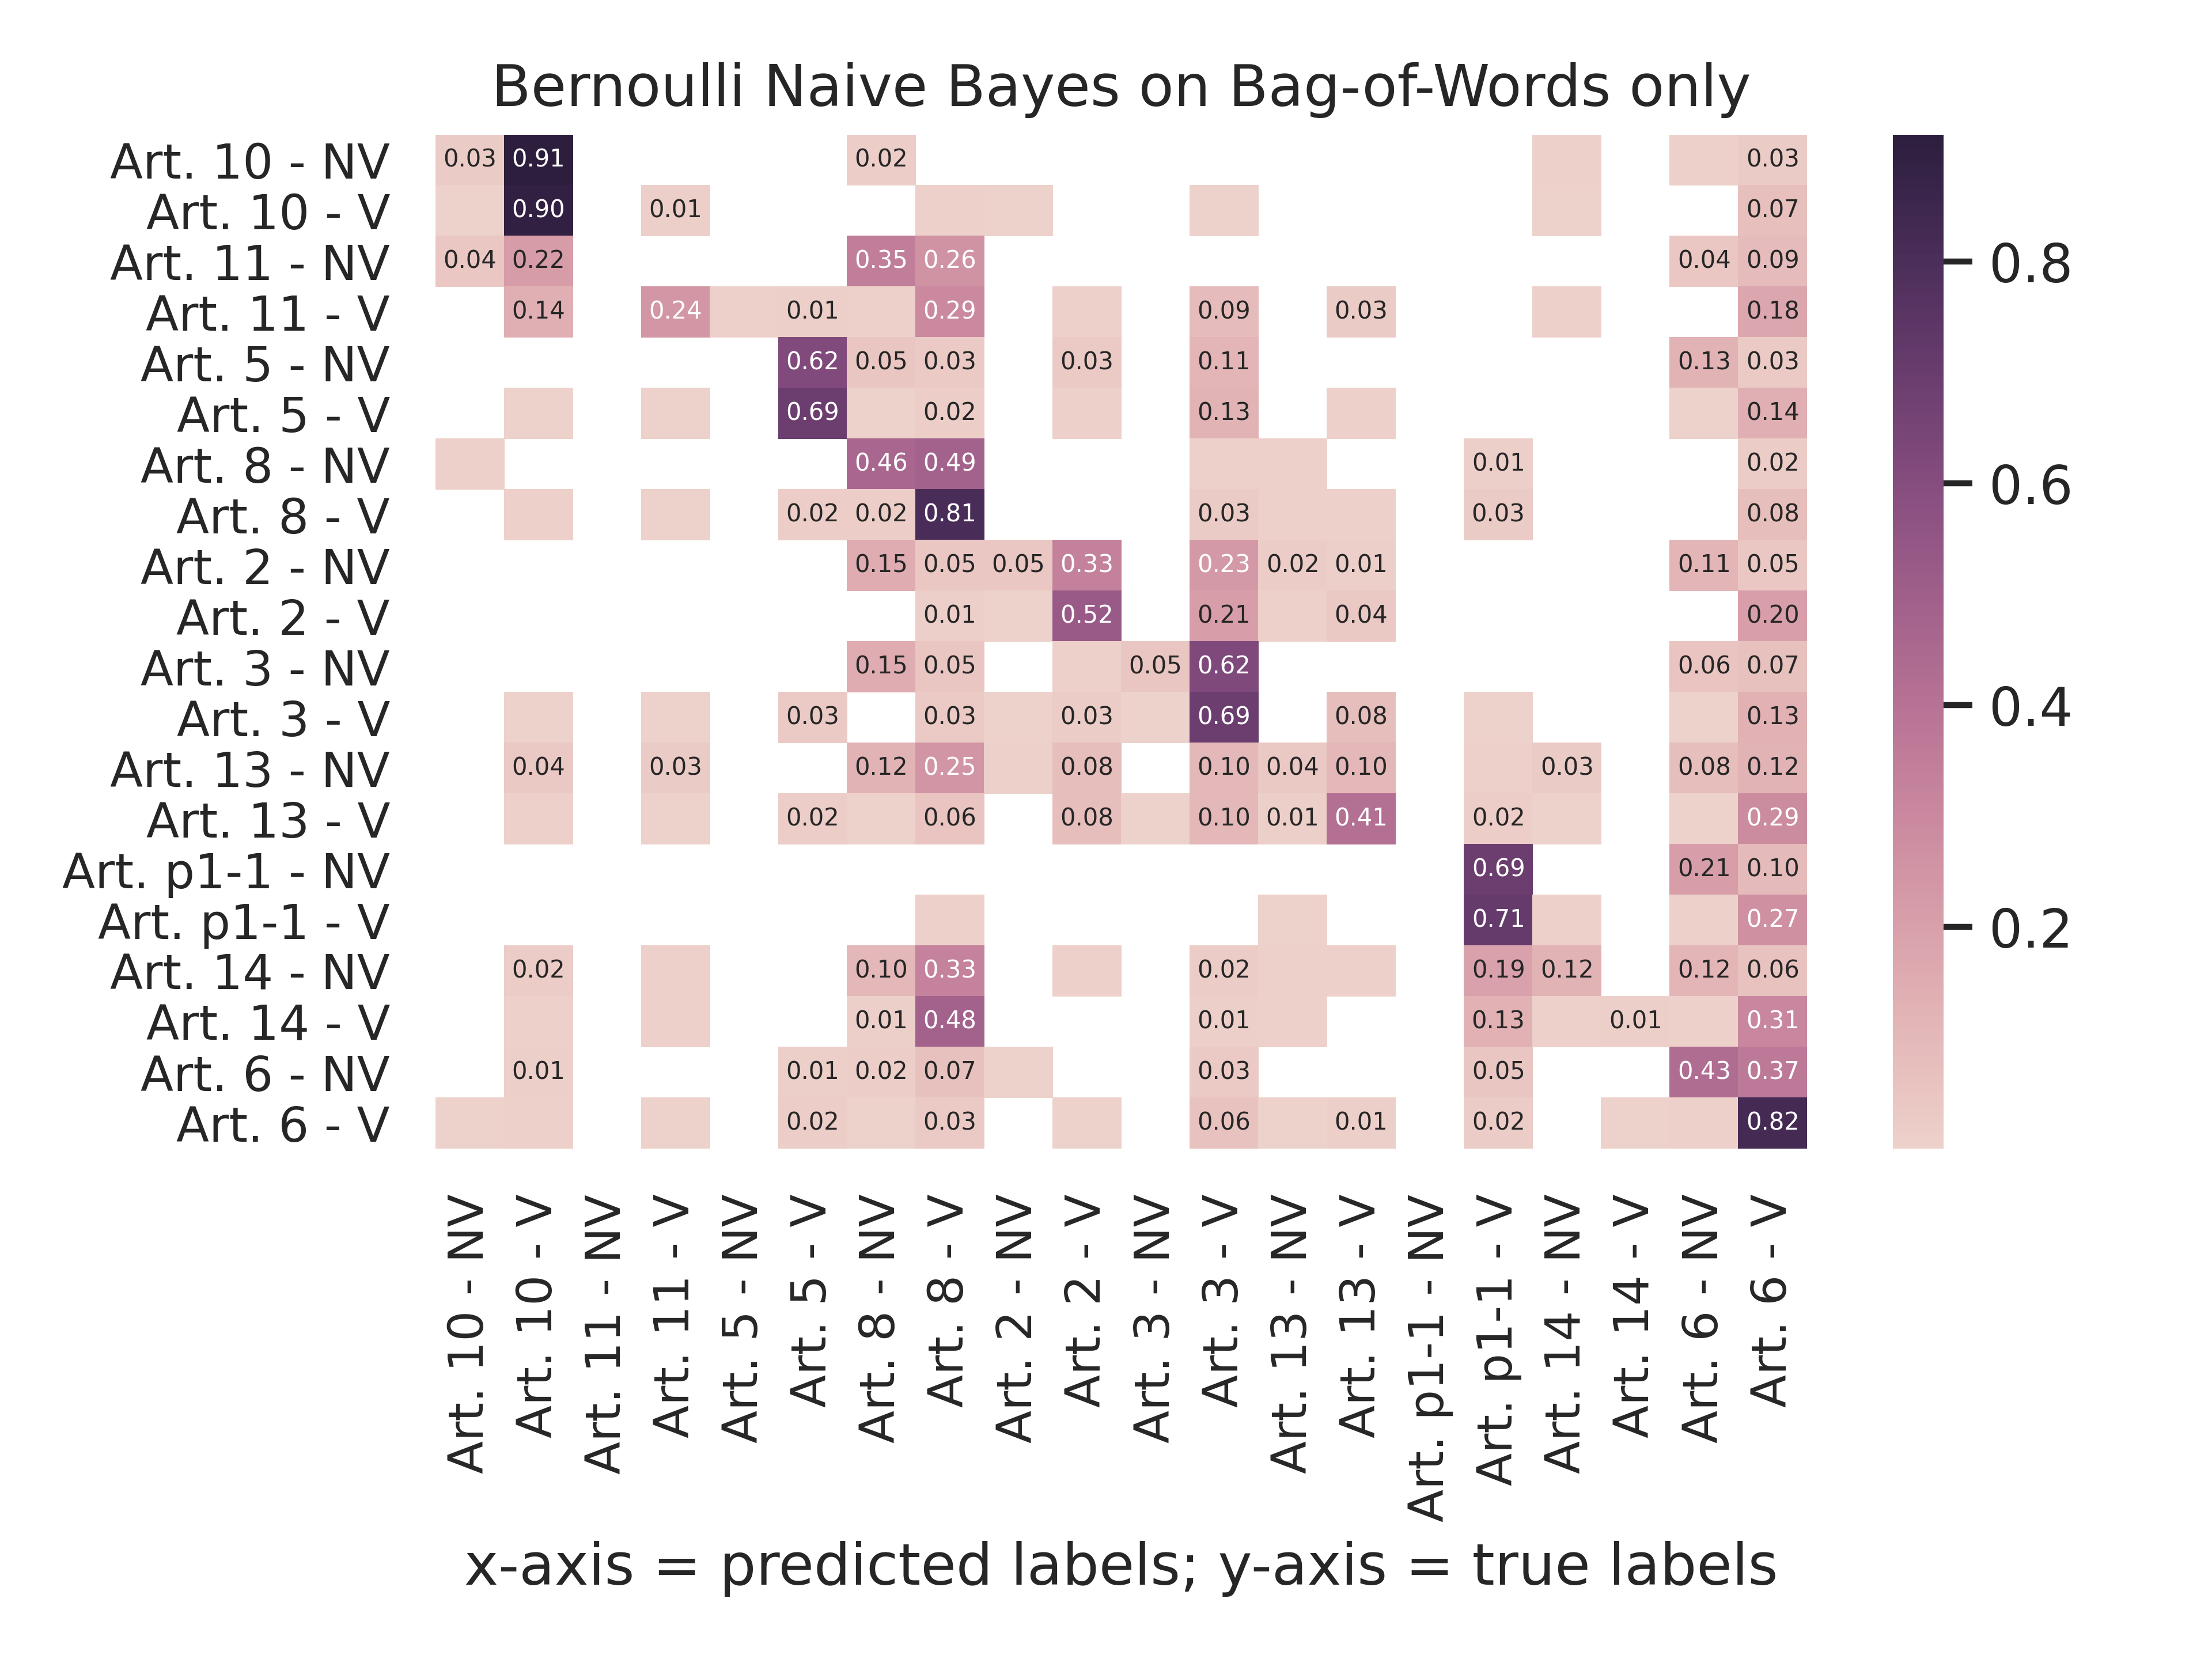
\includegraphics[scale=0.7]{data/analysis/cm/multiclass_cm_test_bernoulli_naive_bayes_bag-of-words_only.png}  
\end{figure}
\begin{figure}[!htb]
    \centering
    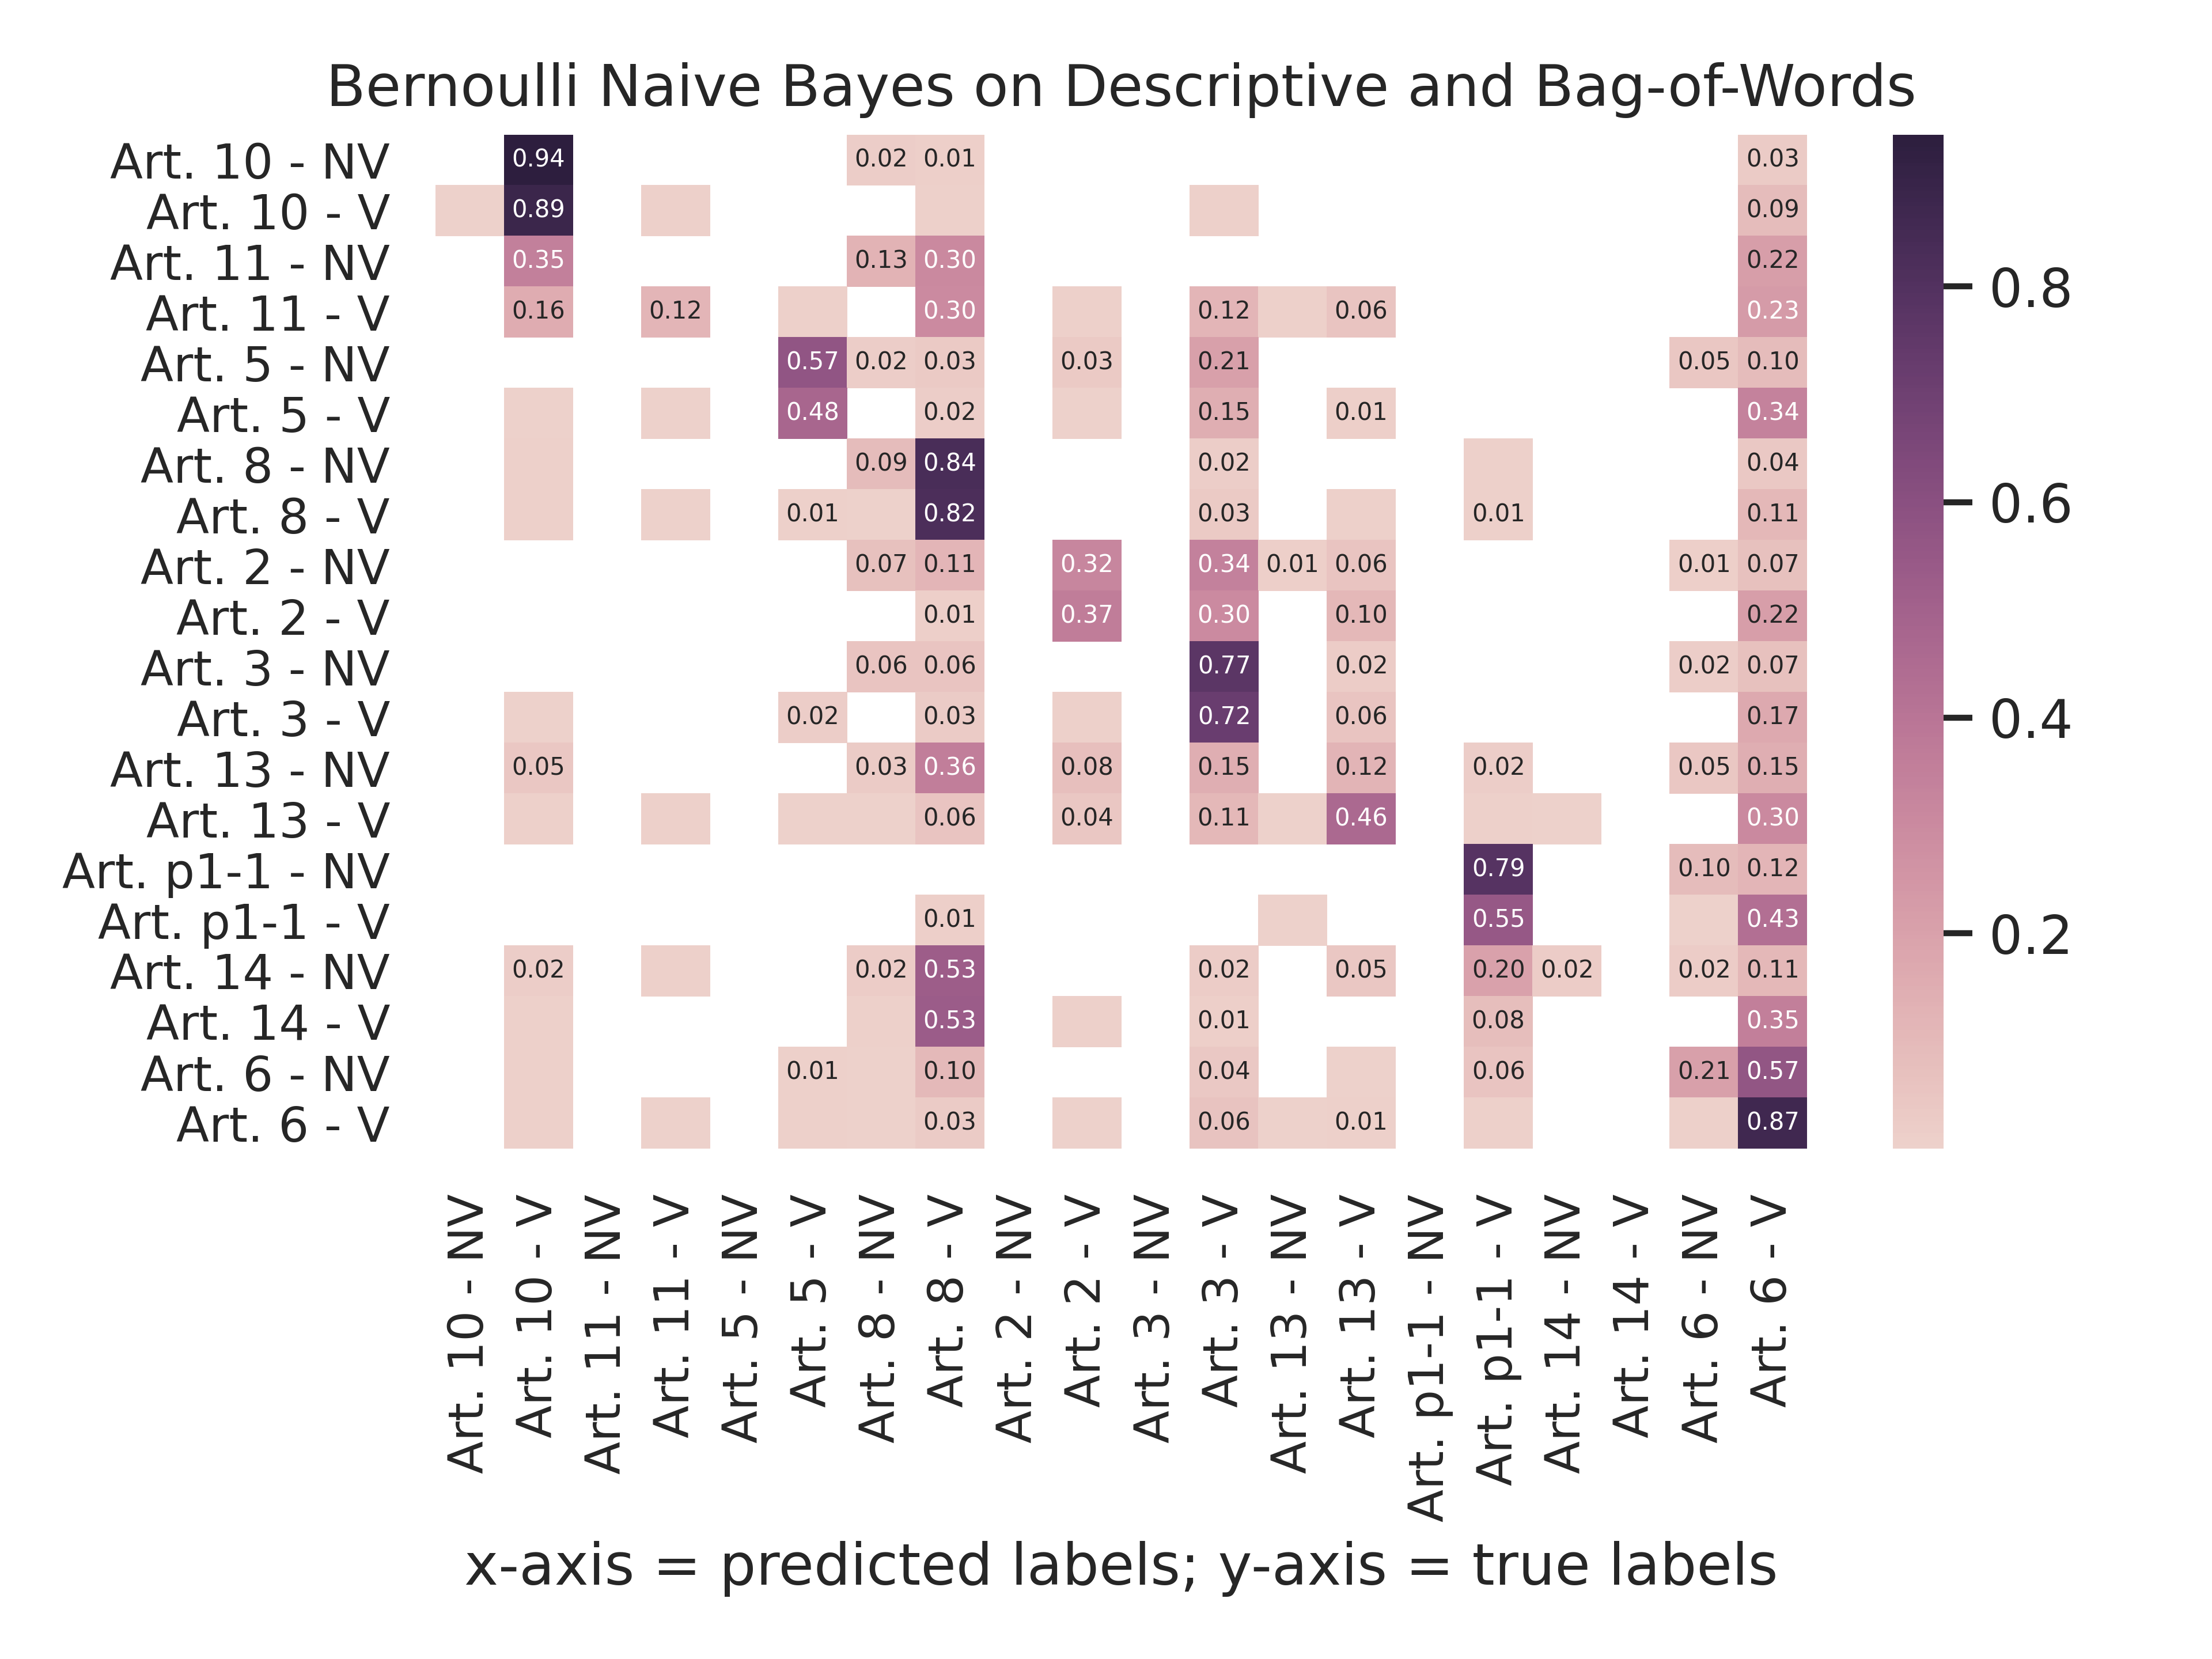
\includegraphics[scale=0.7]{data/analysis/cm/multiclass_cm_test_bernoulli_naive_bayes_descriptive_and_bag-of-words.png}  
\end{figure}
\begin{figure}[!htb]
    \centering
    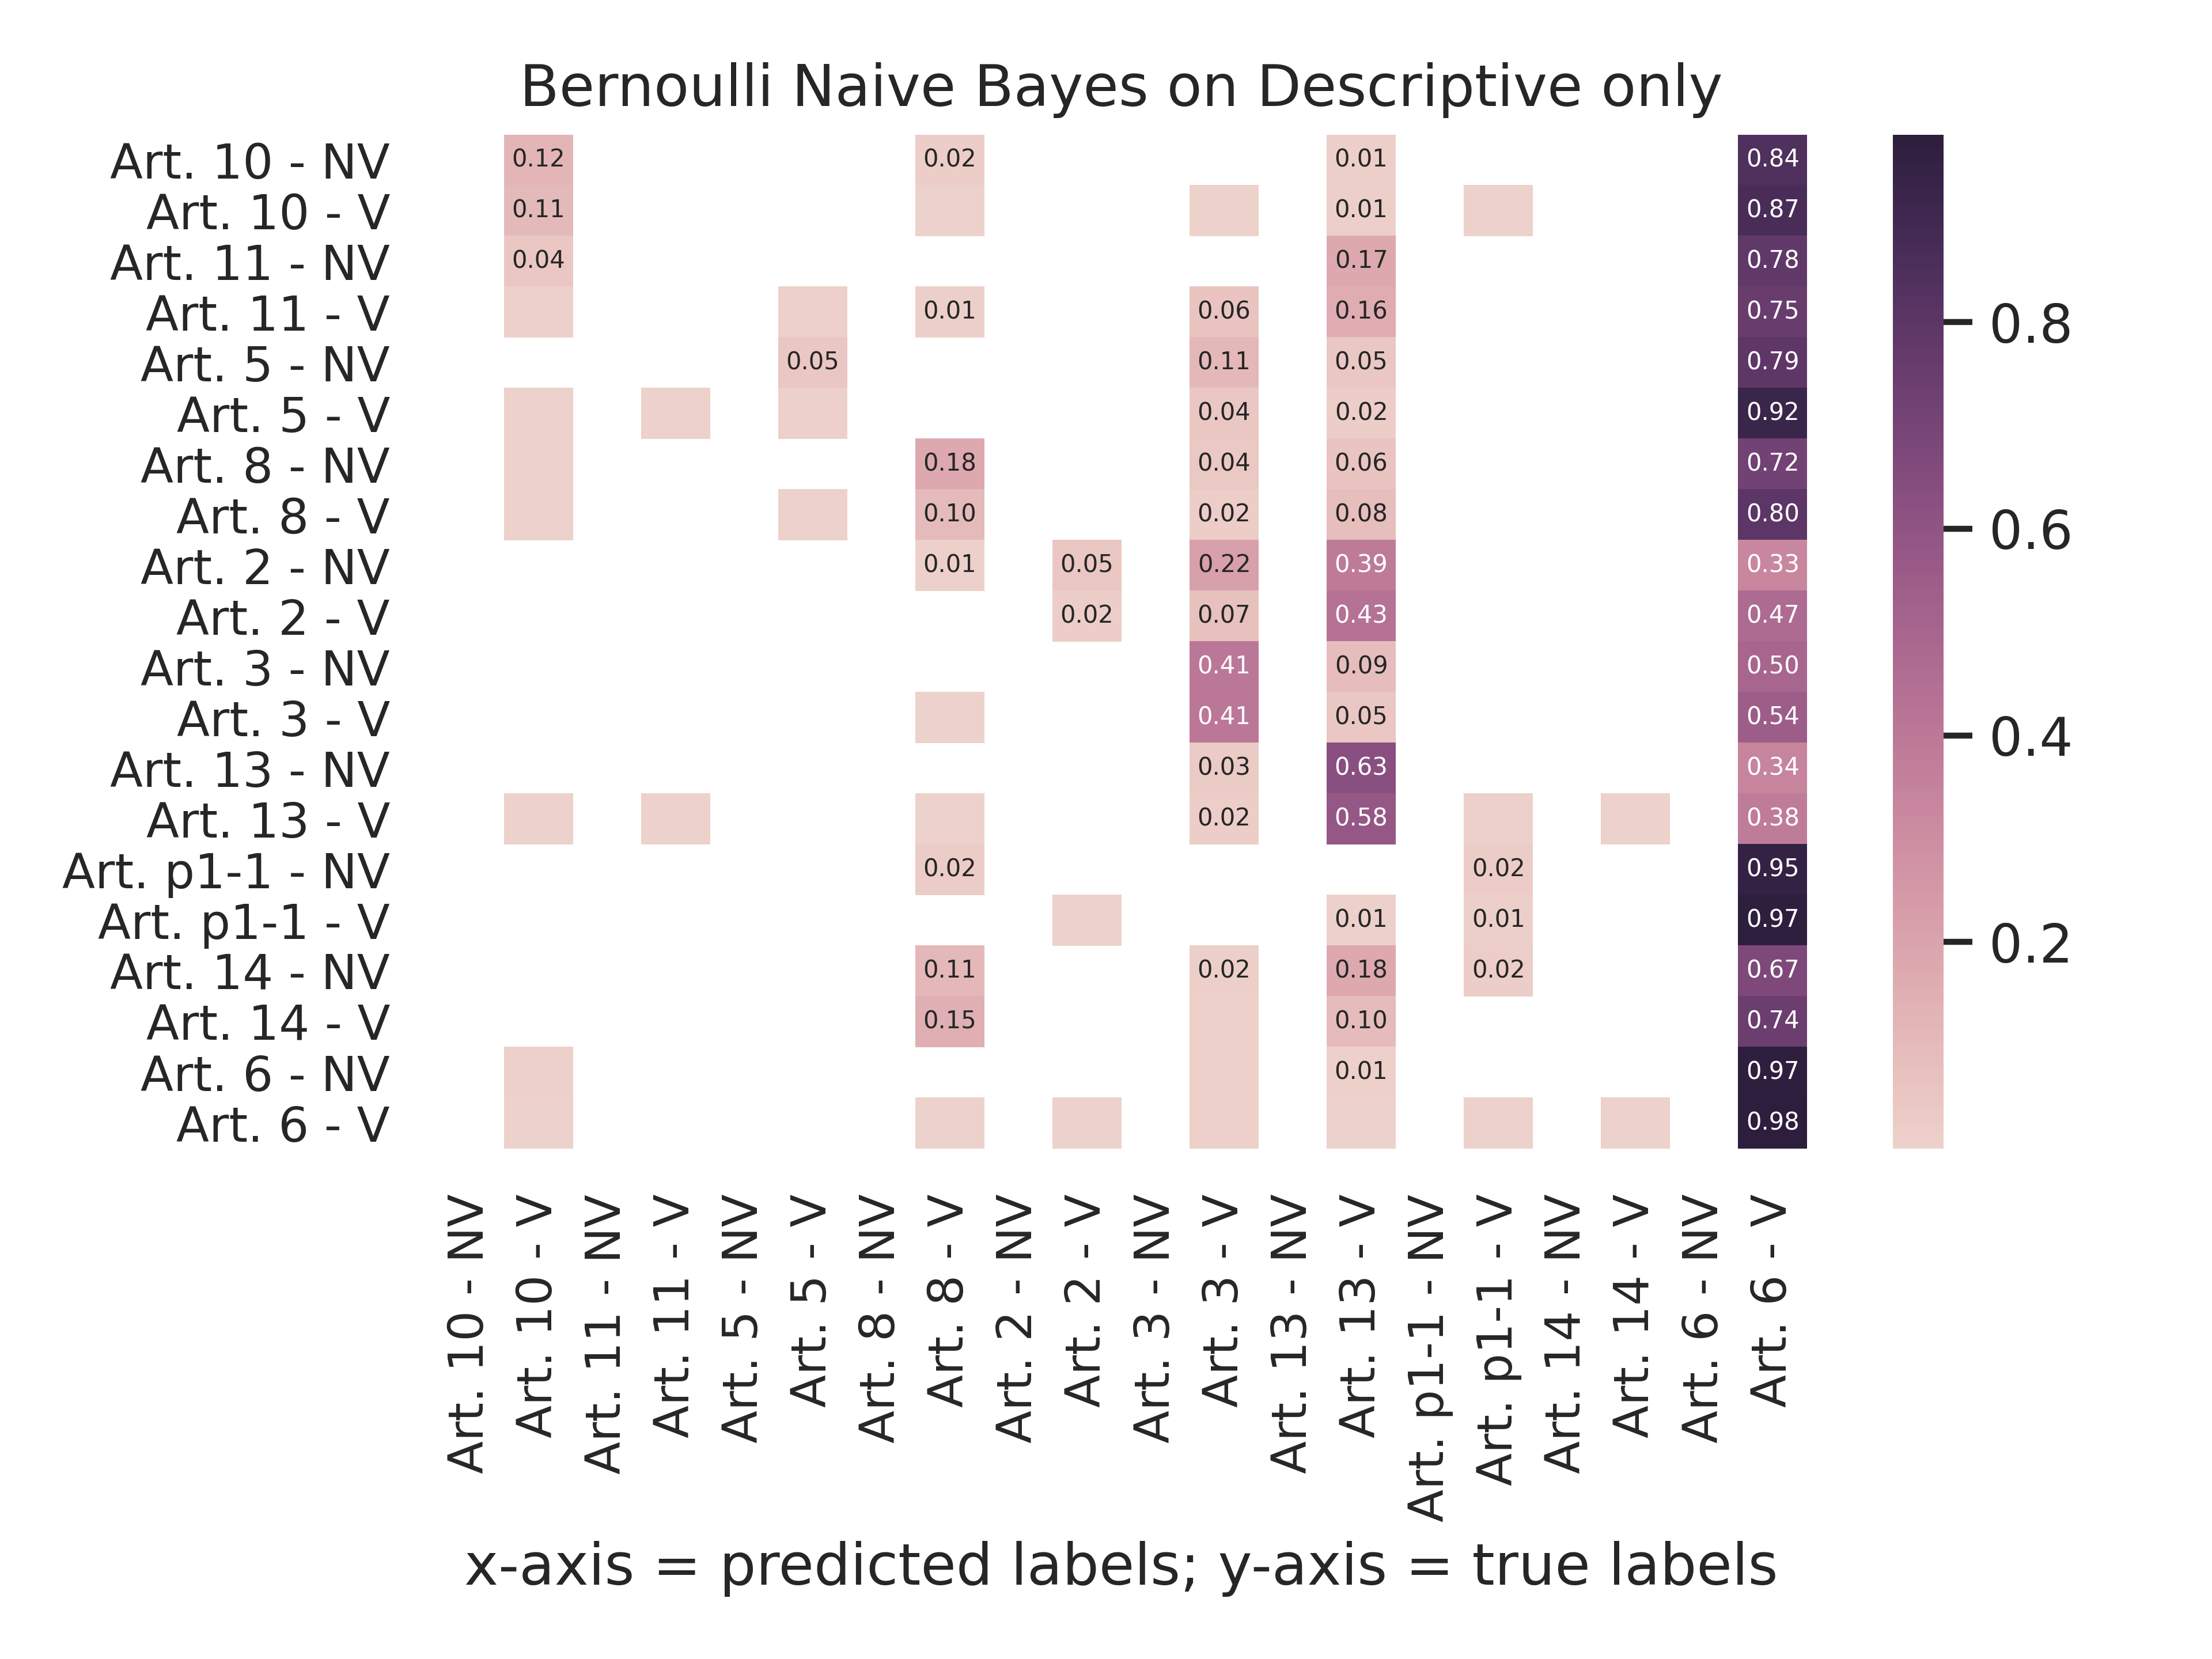
\includegraphics[scale=0.7]{data/analysis/cm/multiclass_cm_test_bernoulli_naive_bayes_descriptive_only.png}  
\end{figure}
\begin{figure}[!htb]
    \centering
    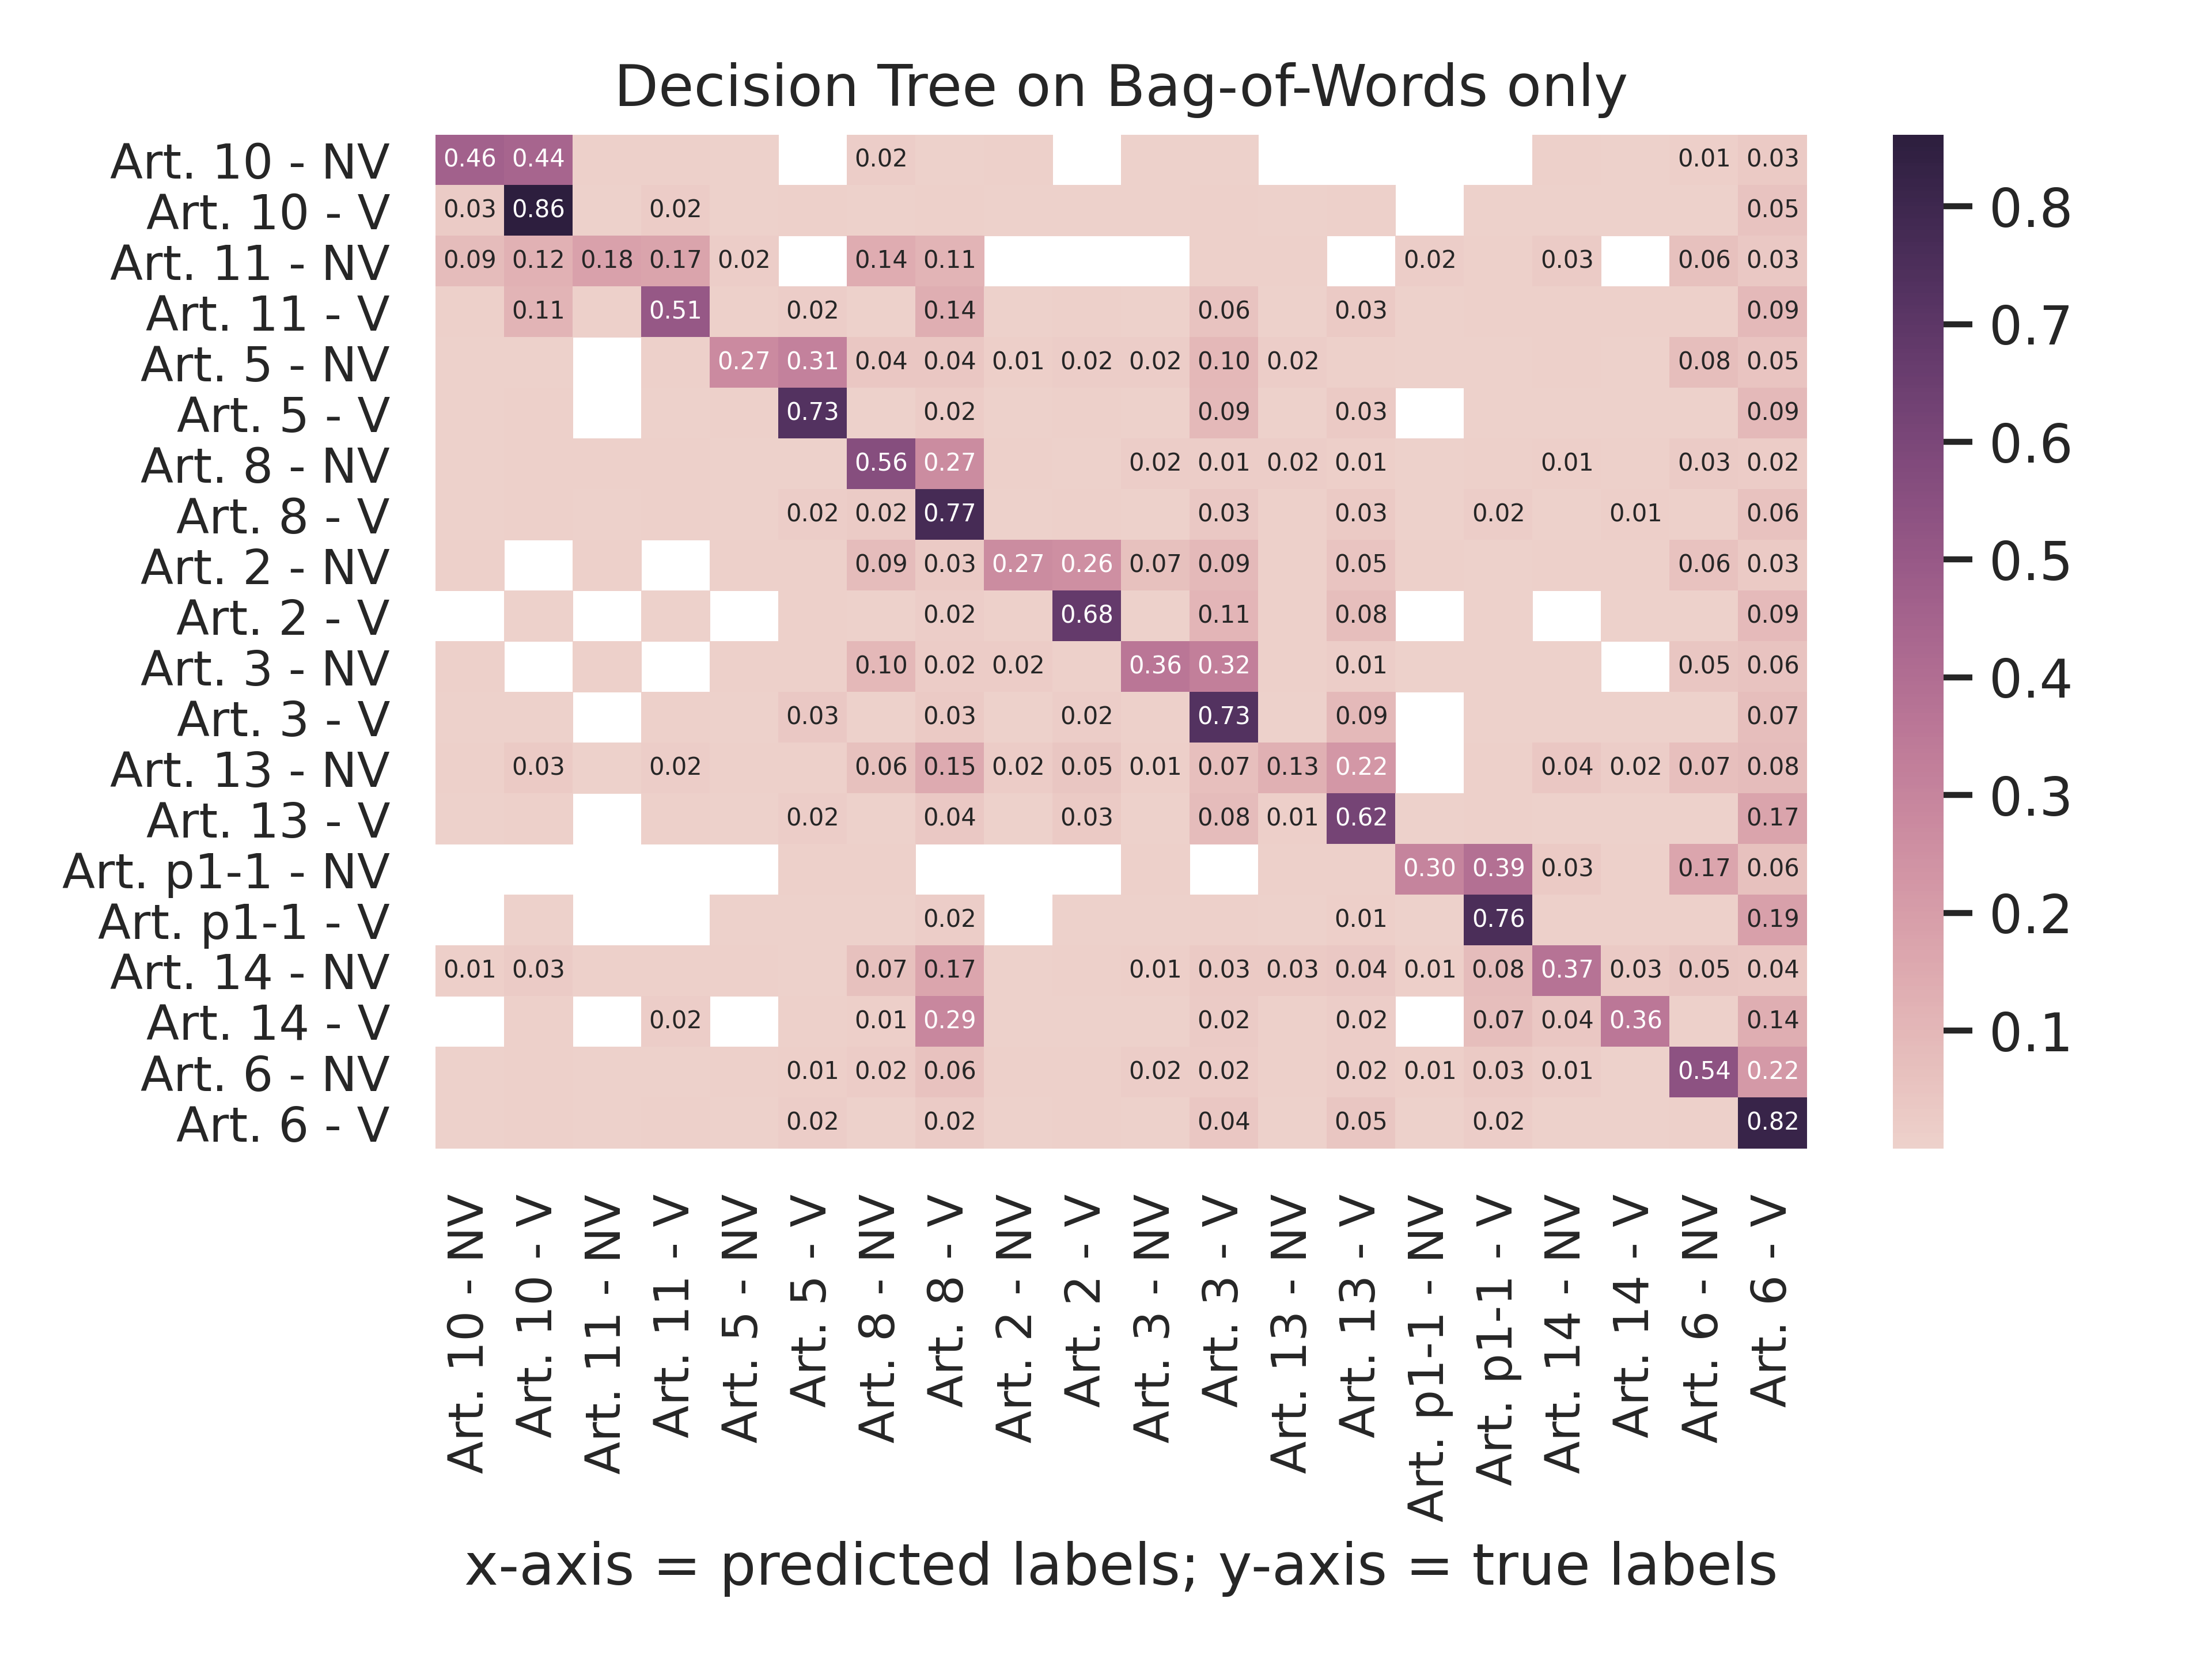
\includegraphics[scale=0.7]{data/analysis/cm/multiclass_cm_test_decision_tree_bag-of-words_only.png}  
\end{figure}
\begin{figure}[!htb]
    \centering
    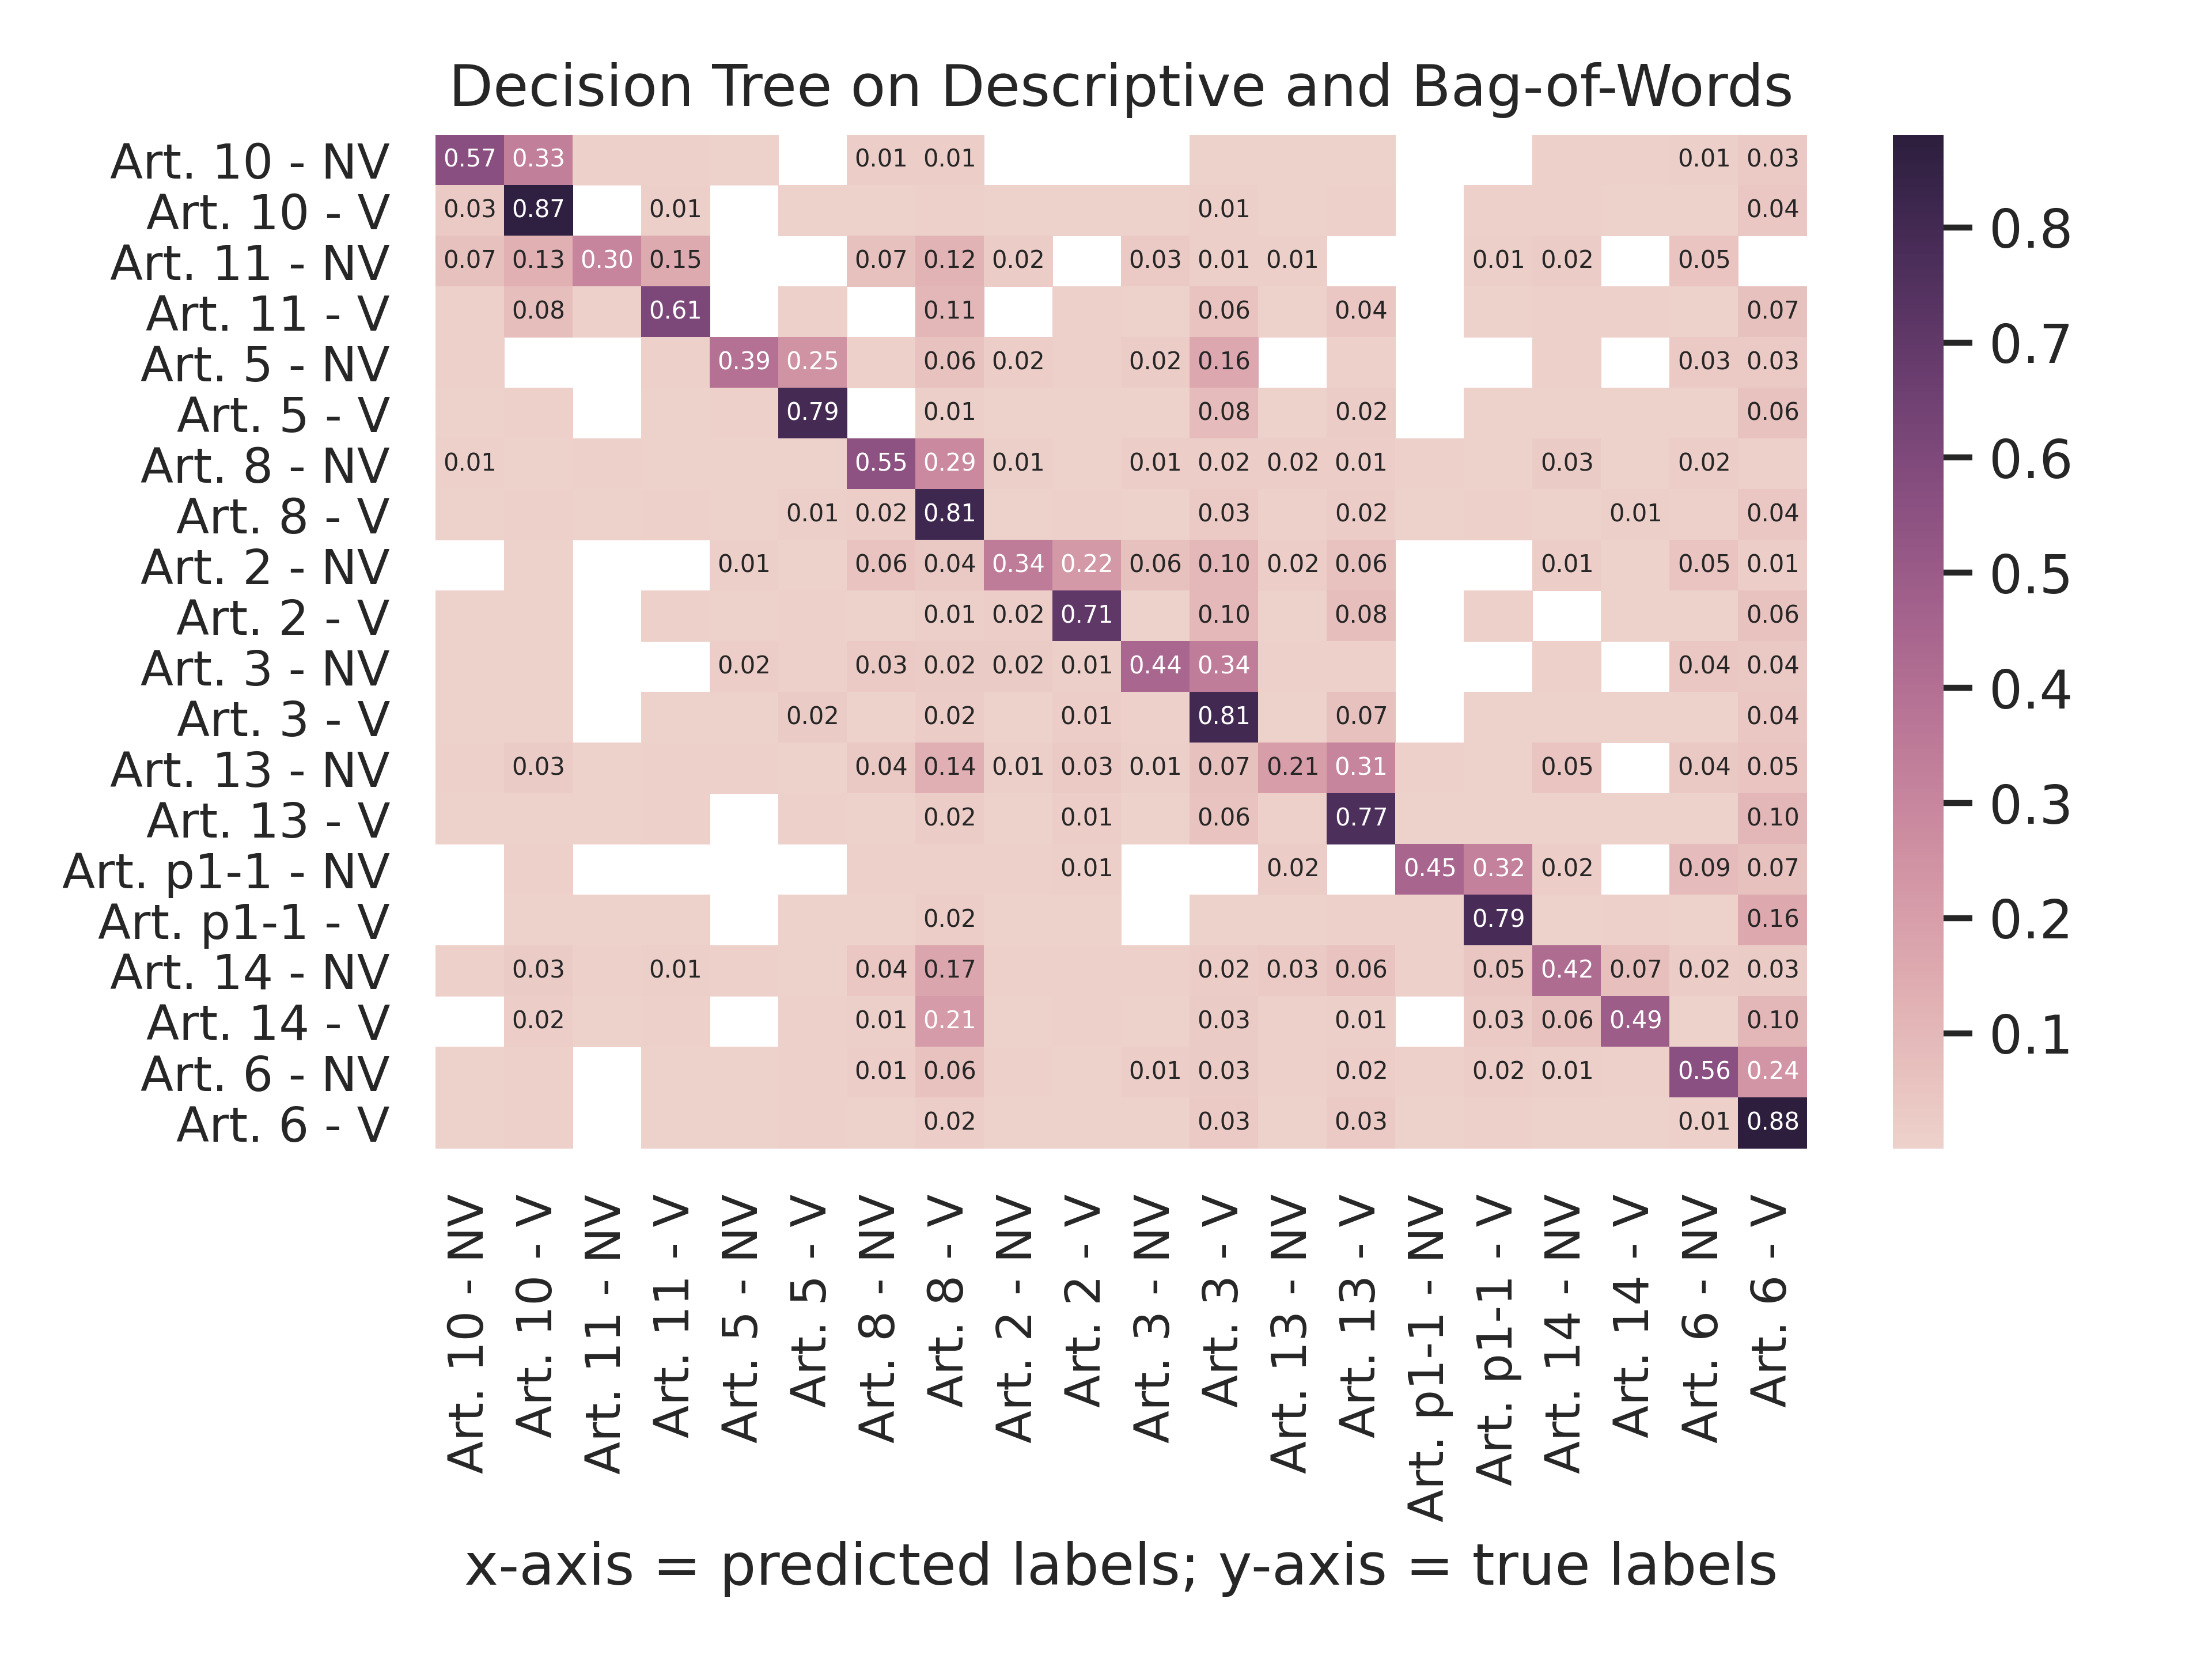
\includegraphics[scale=0.7]{data/analysis/cm/multiclass_cm_test_decision_tree_descriptive_and_bag-of-words.png}  
\end{figure}
\begin{figure}[!htb]
    \centering
    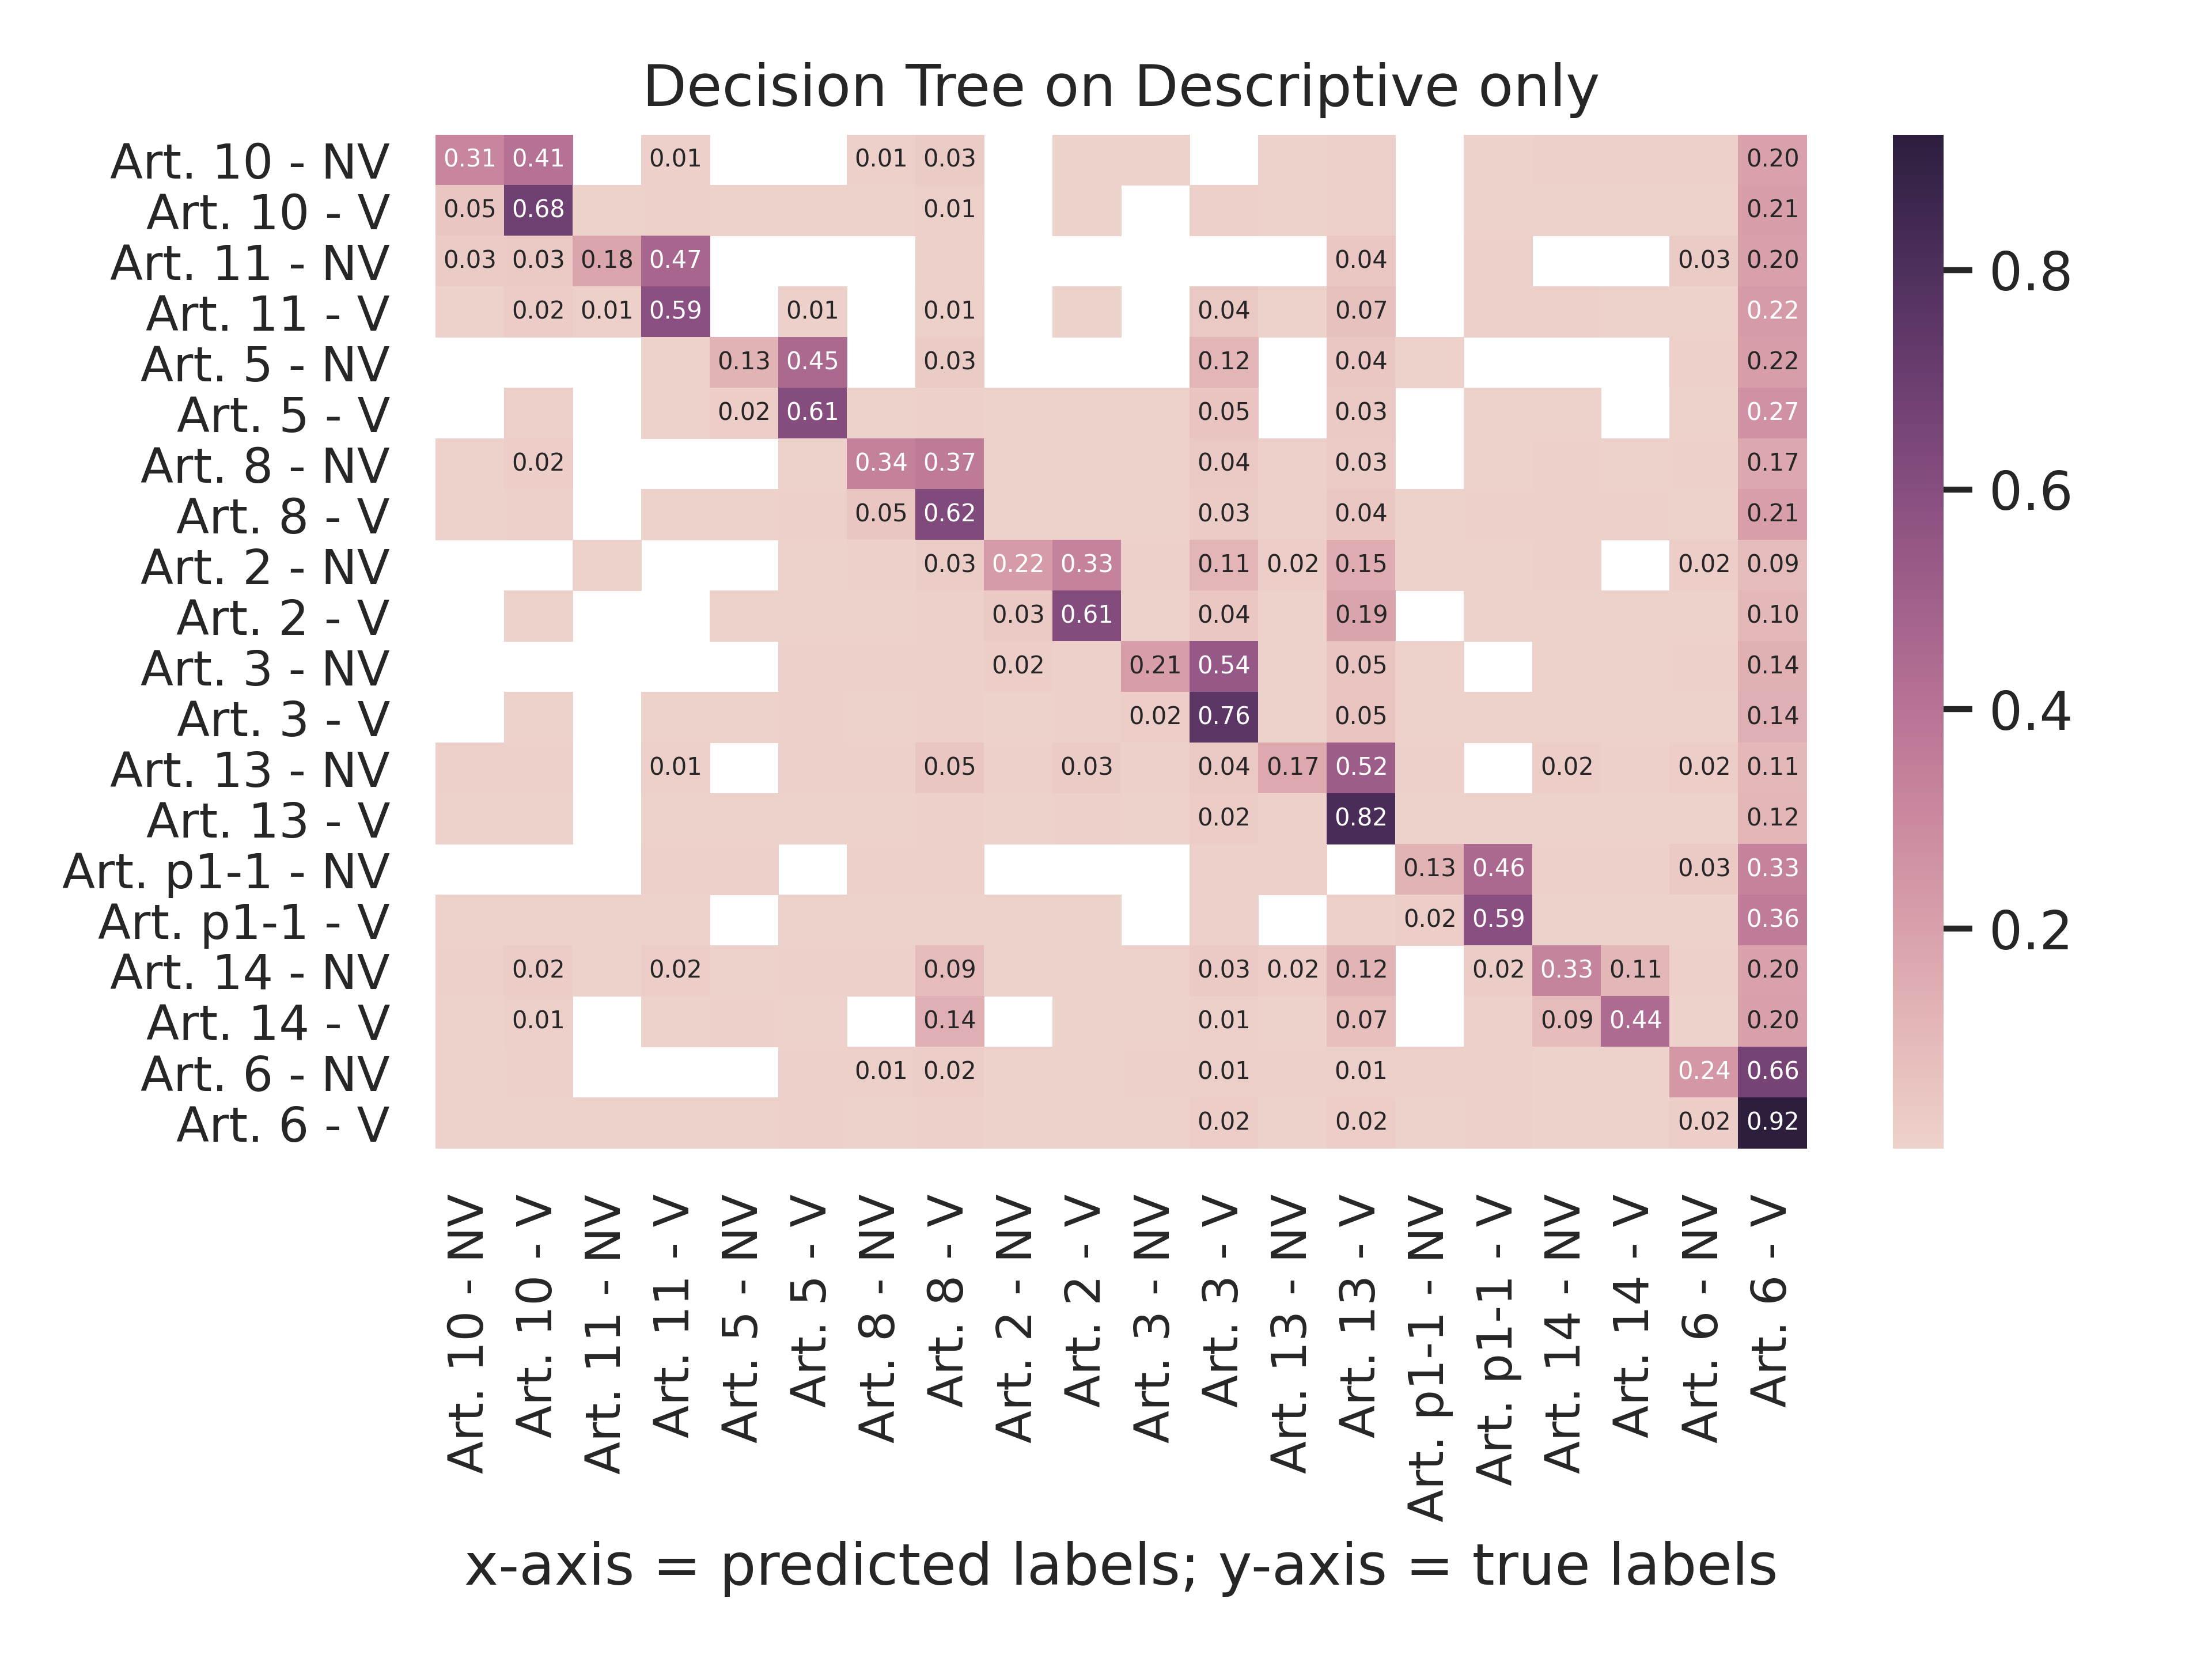
\includegraphics[scale=0.7]{data/analysis/cm/multiclass_cm_test_decision_tree_descriptive_only.png}  
\end{figure}
\begin{figure}[!htb]
    \centering
    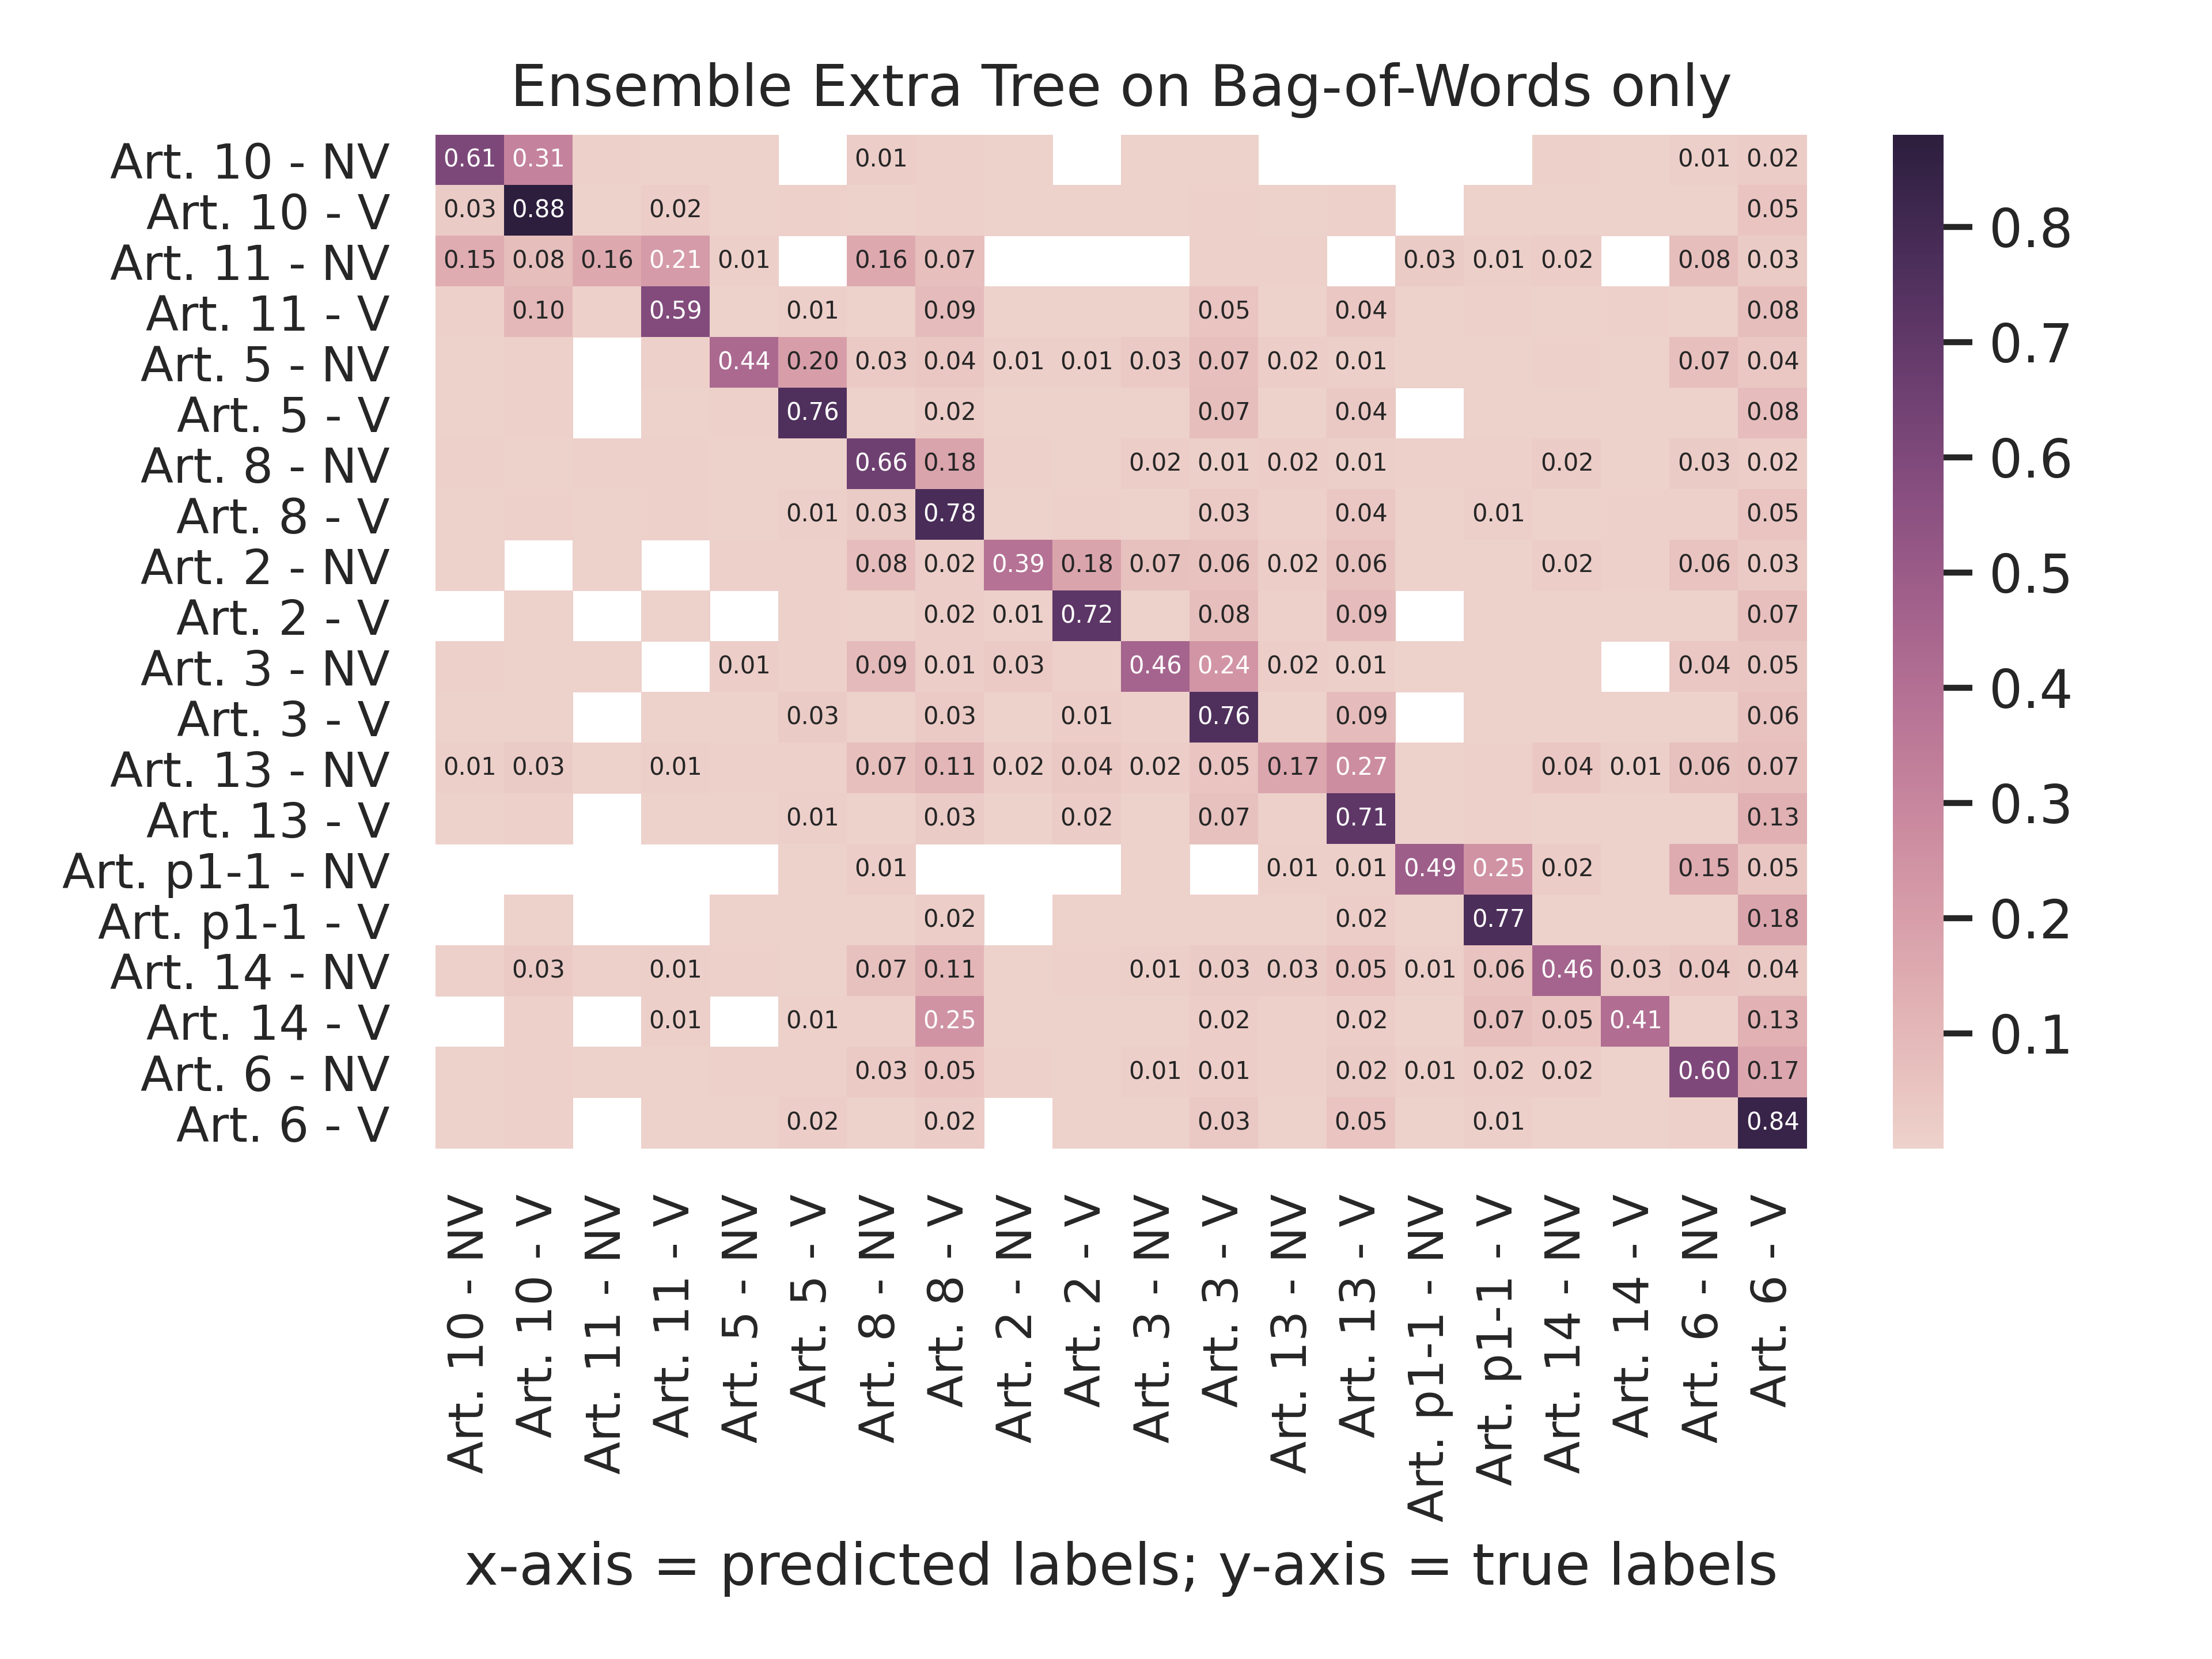
\includegraphics[scale=0.7]{data/analysis/cm/multiclass_cm_test_ensemble_extra_tree_bag-of-words_only.png}  
\end{figure}
\begin{figure}[!htb]
    \centering
    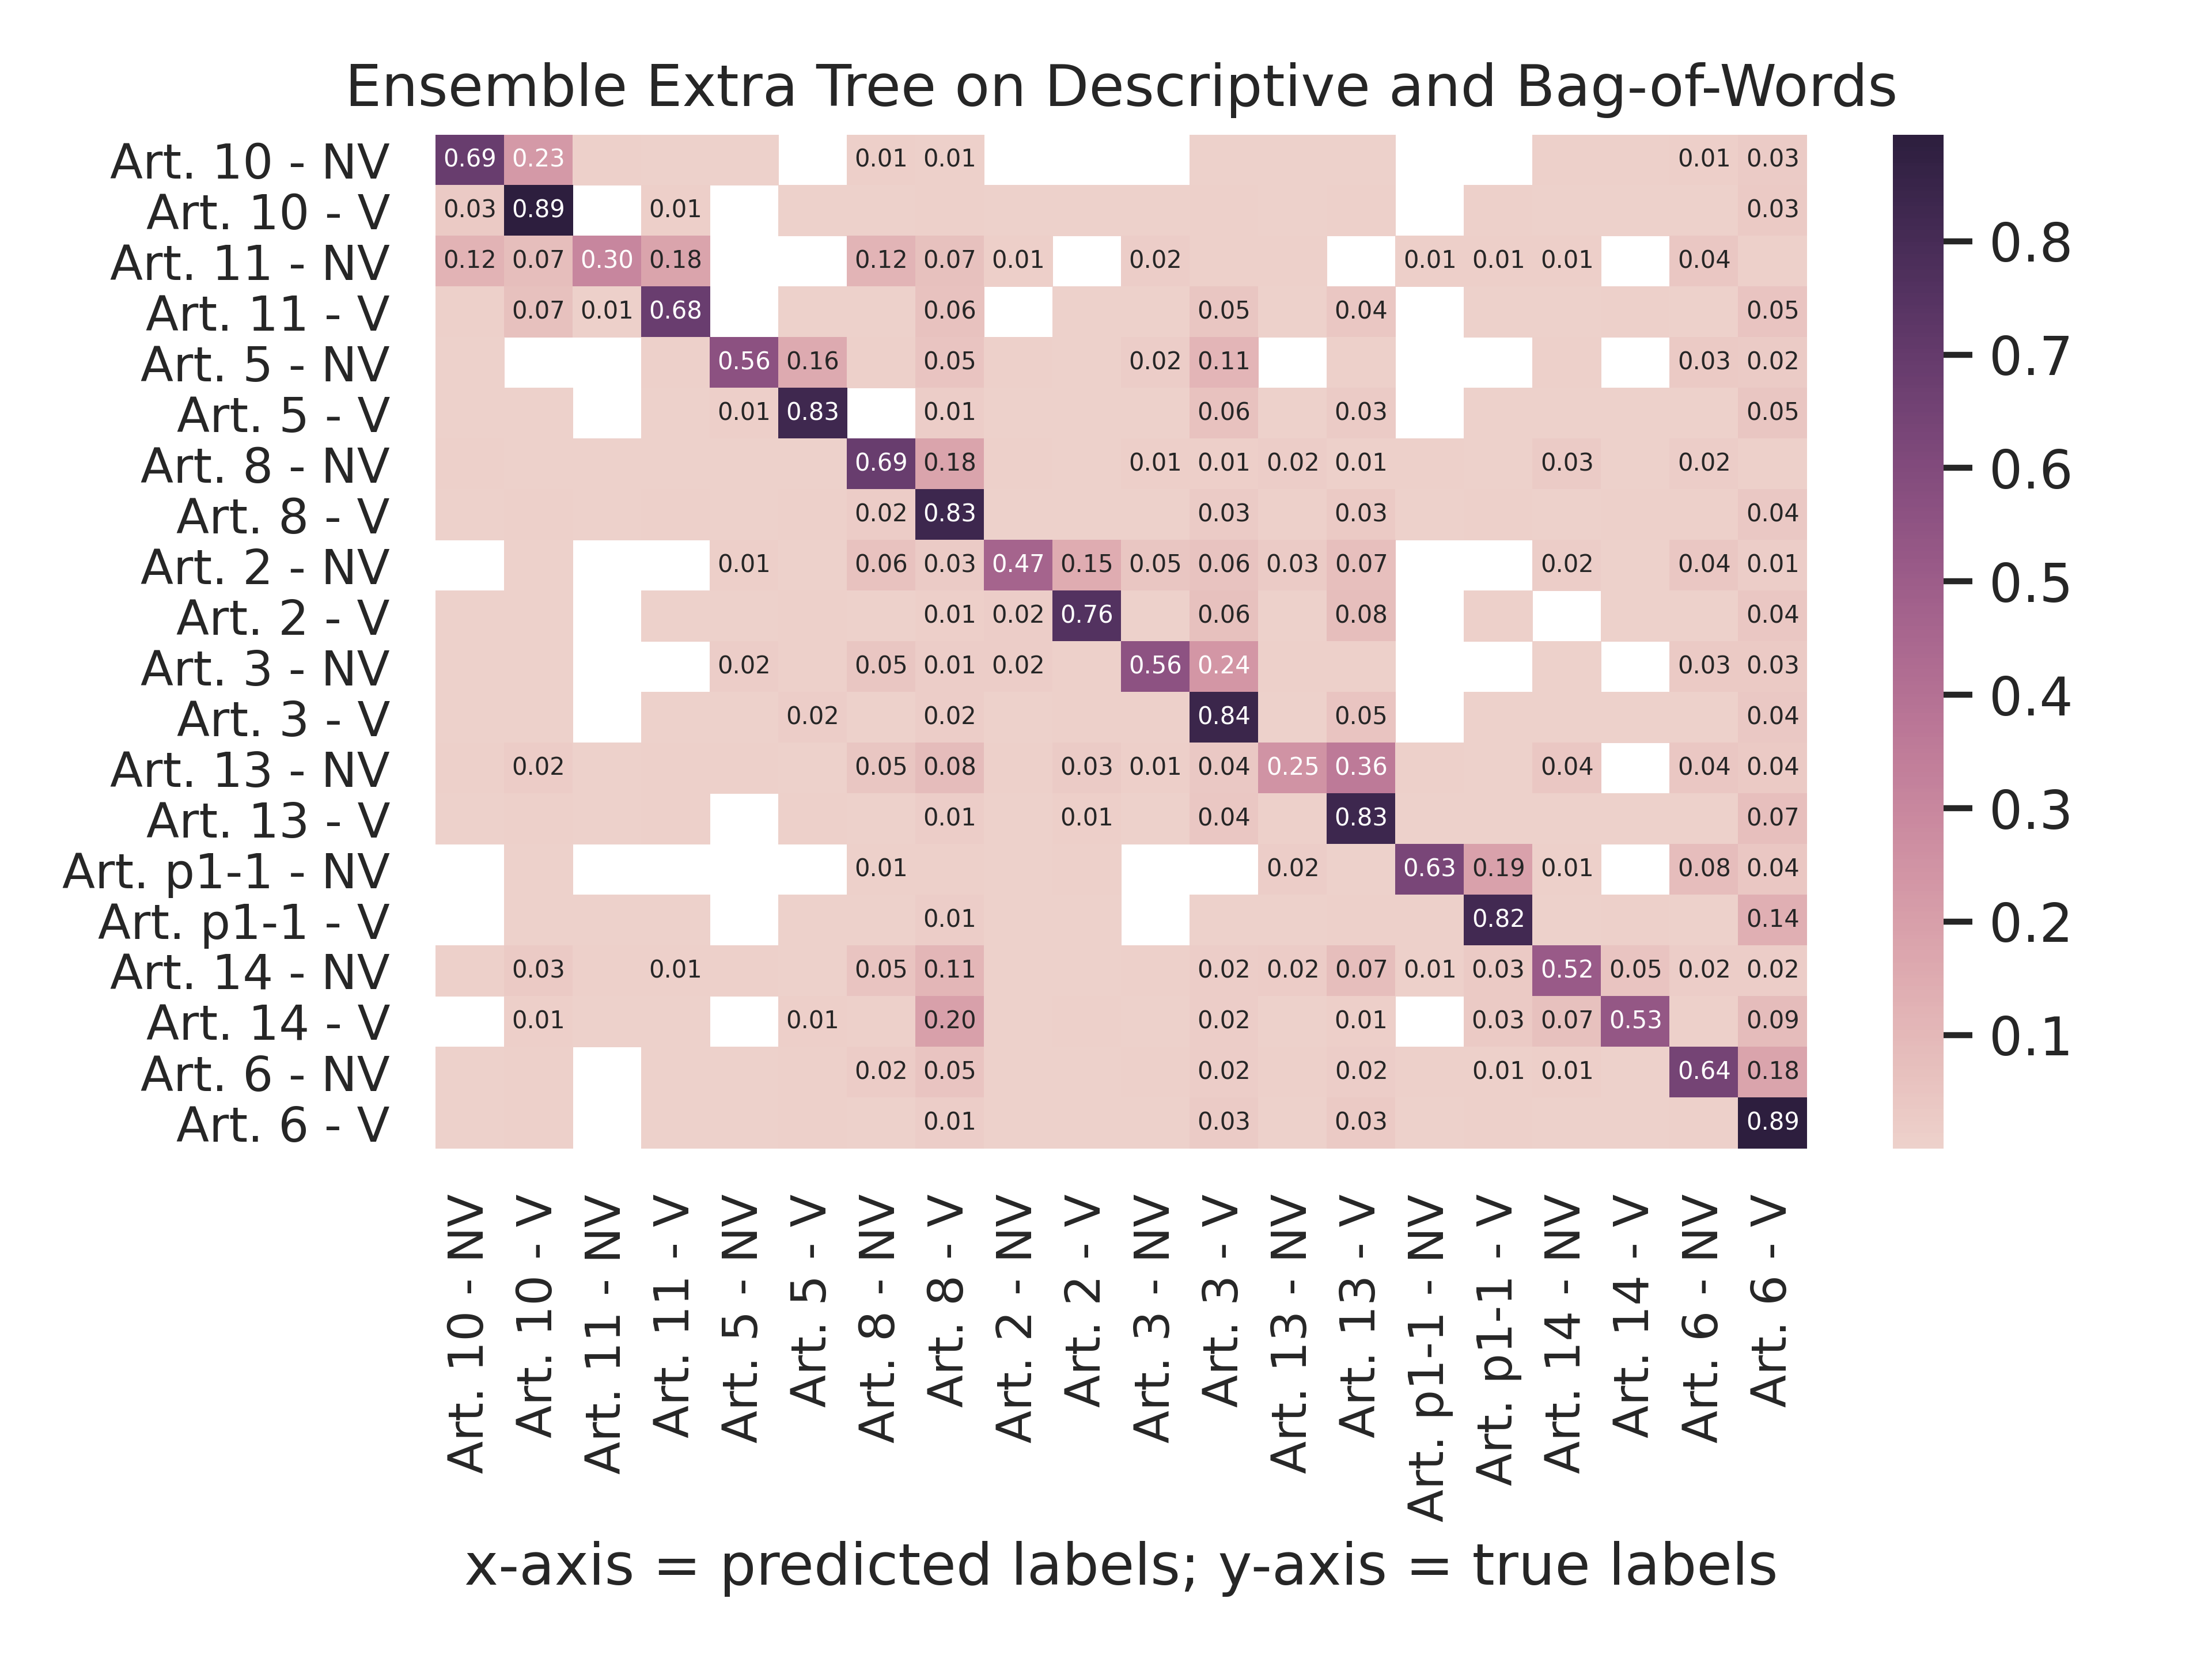
\includegraphics[scale=0.7]{data/analysis/cm/multiclass_cm_test_ensemble_extra_tree_descriptive_and_bag-of-words.png}  
\end{figure}
\begin{figure}[!htb]
    \centering
    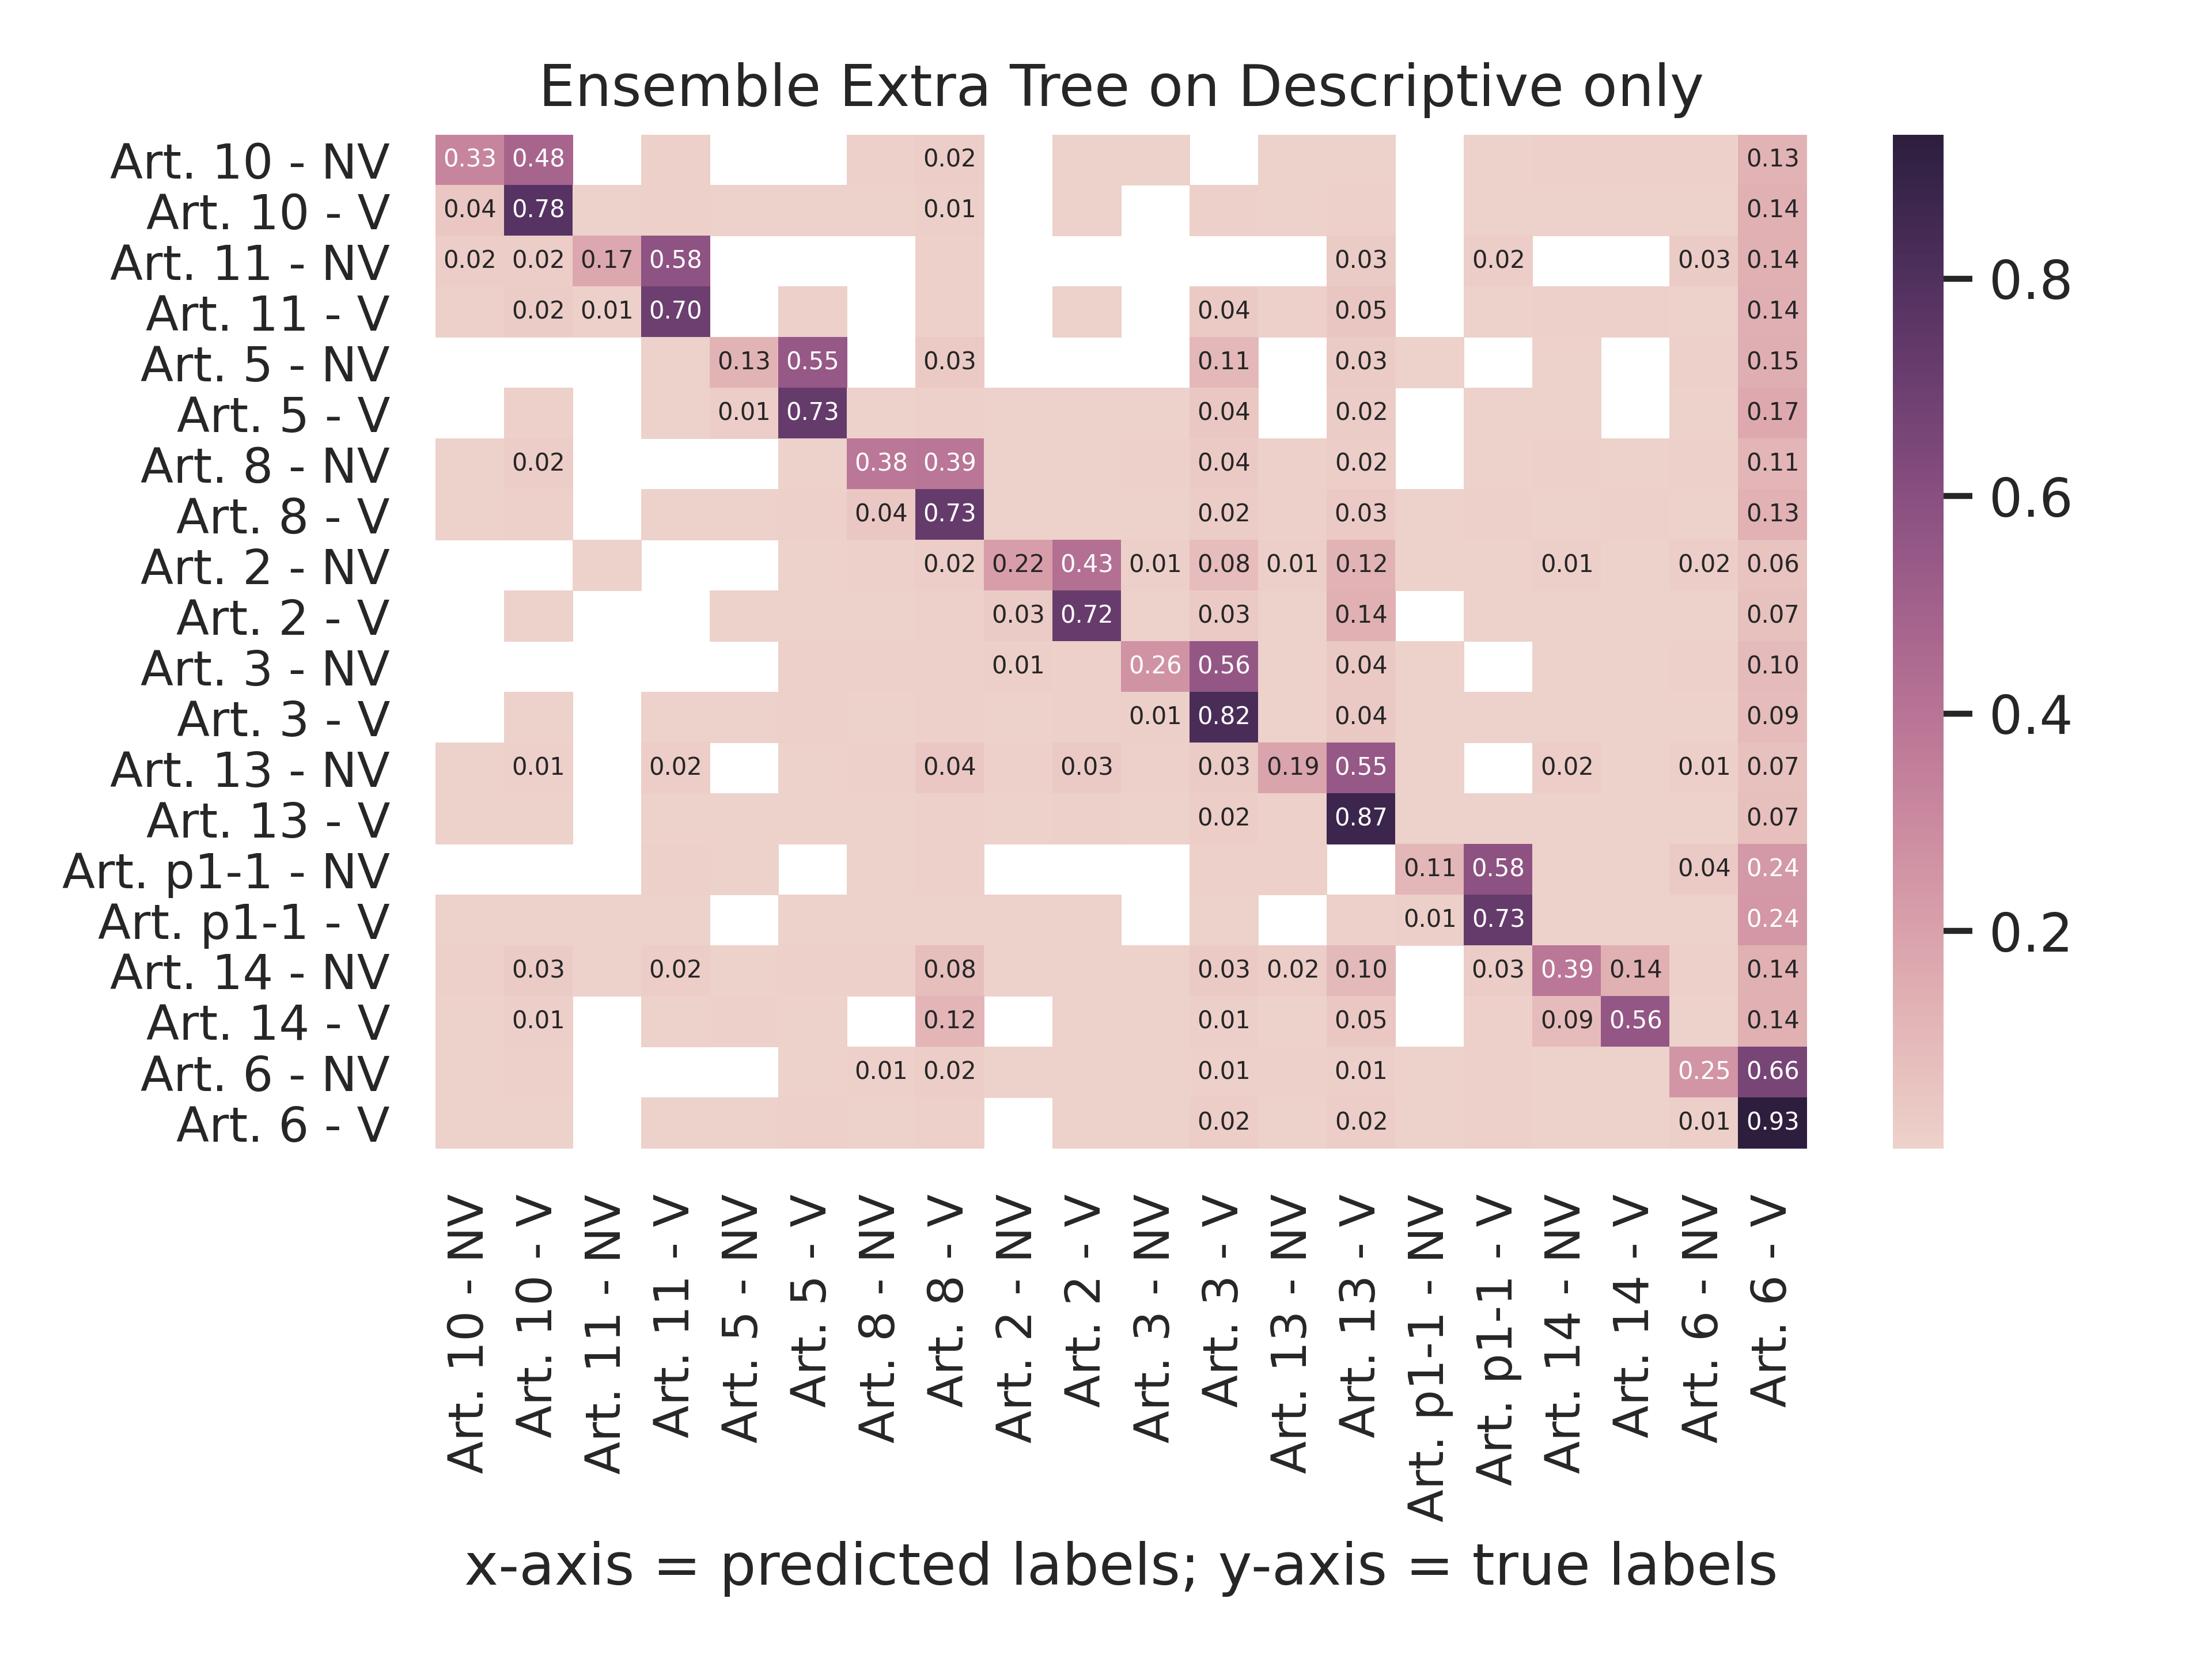
\includegraphics[scale=0.7]{data/analysis/cm/multiclass_cm_test_ensemble_extra_tree_descriptive_only.png}  
\end{figure}
\begin{figure}[!htb]
    \centering
    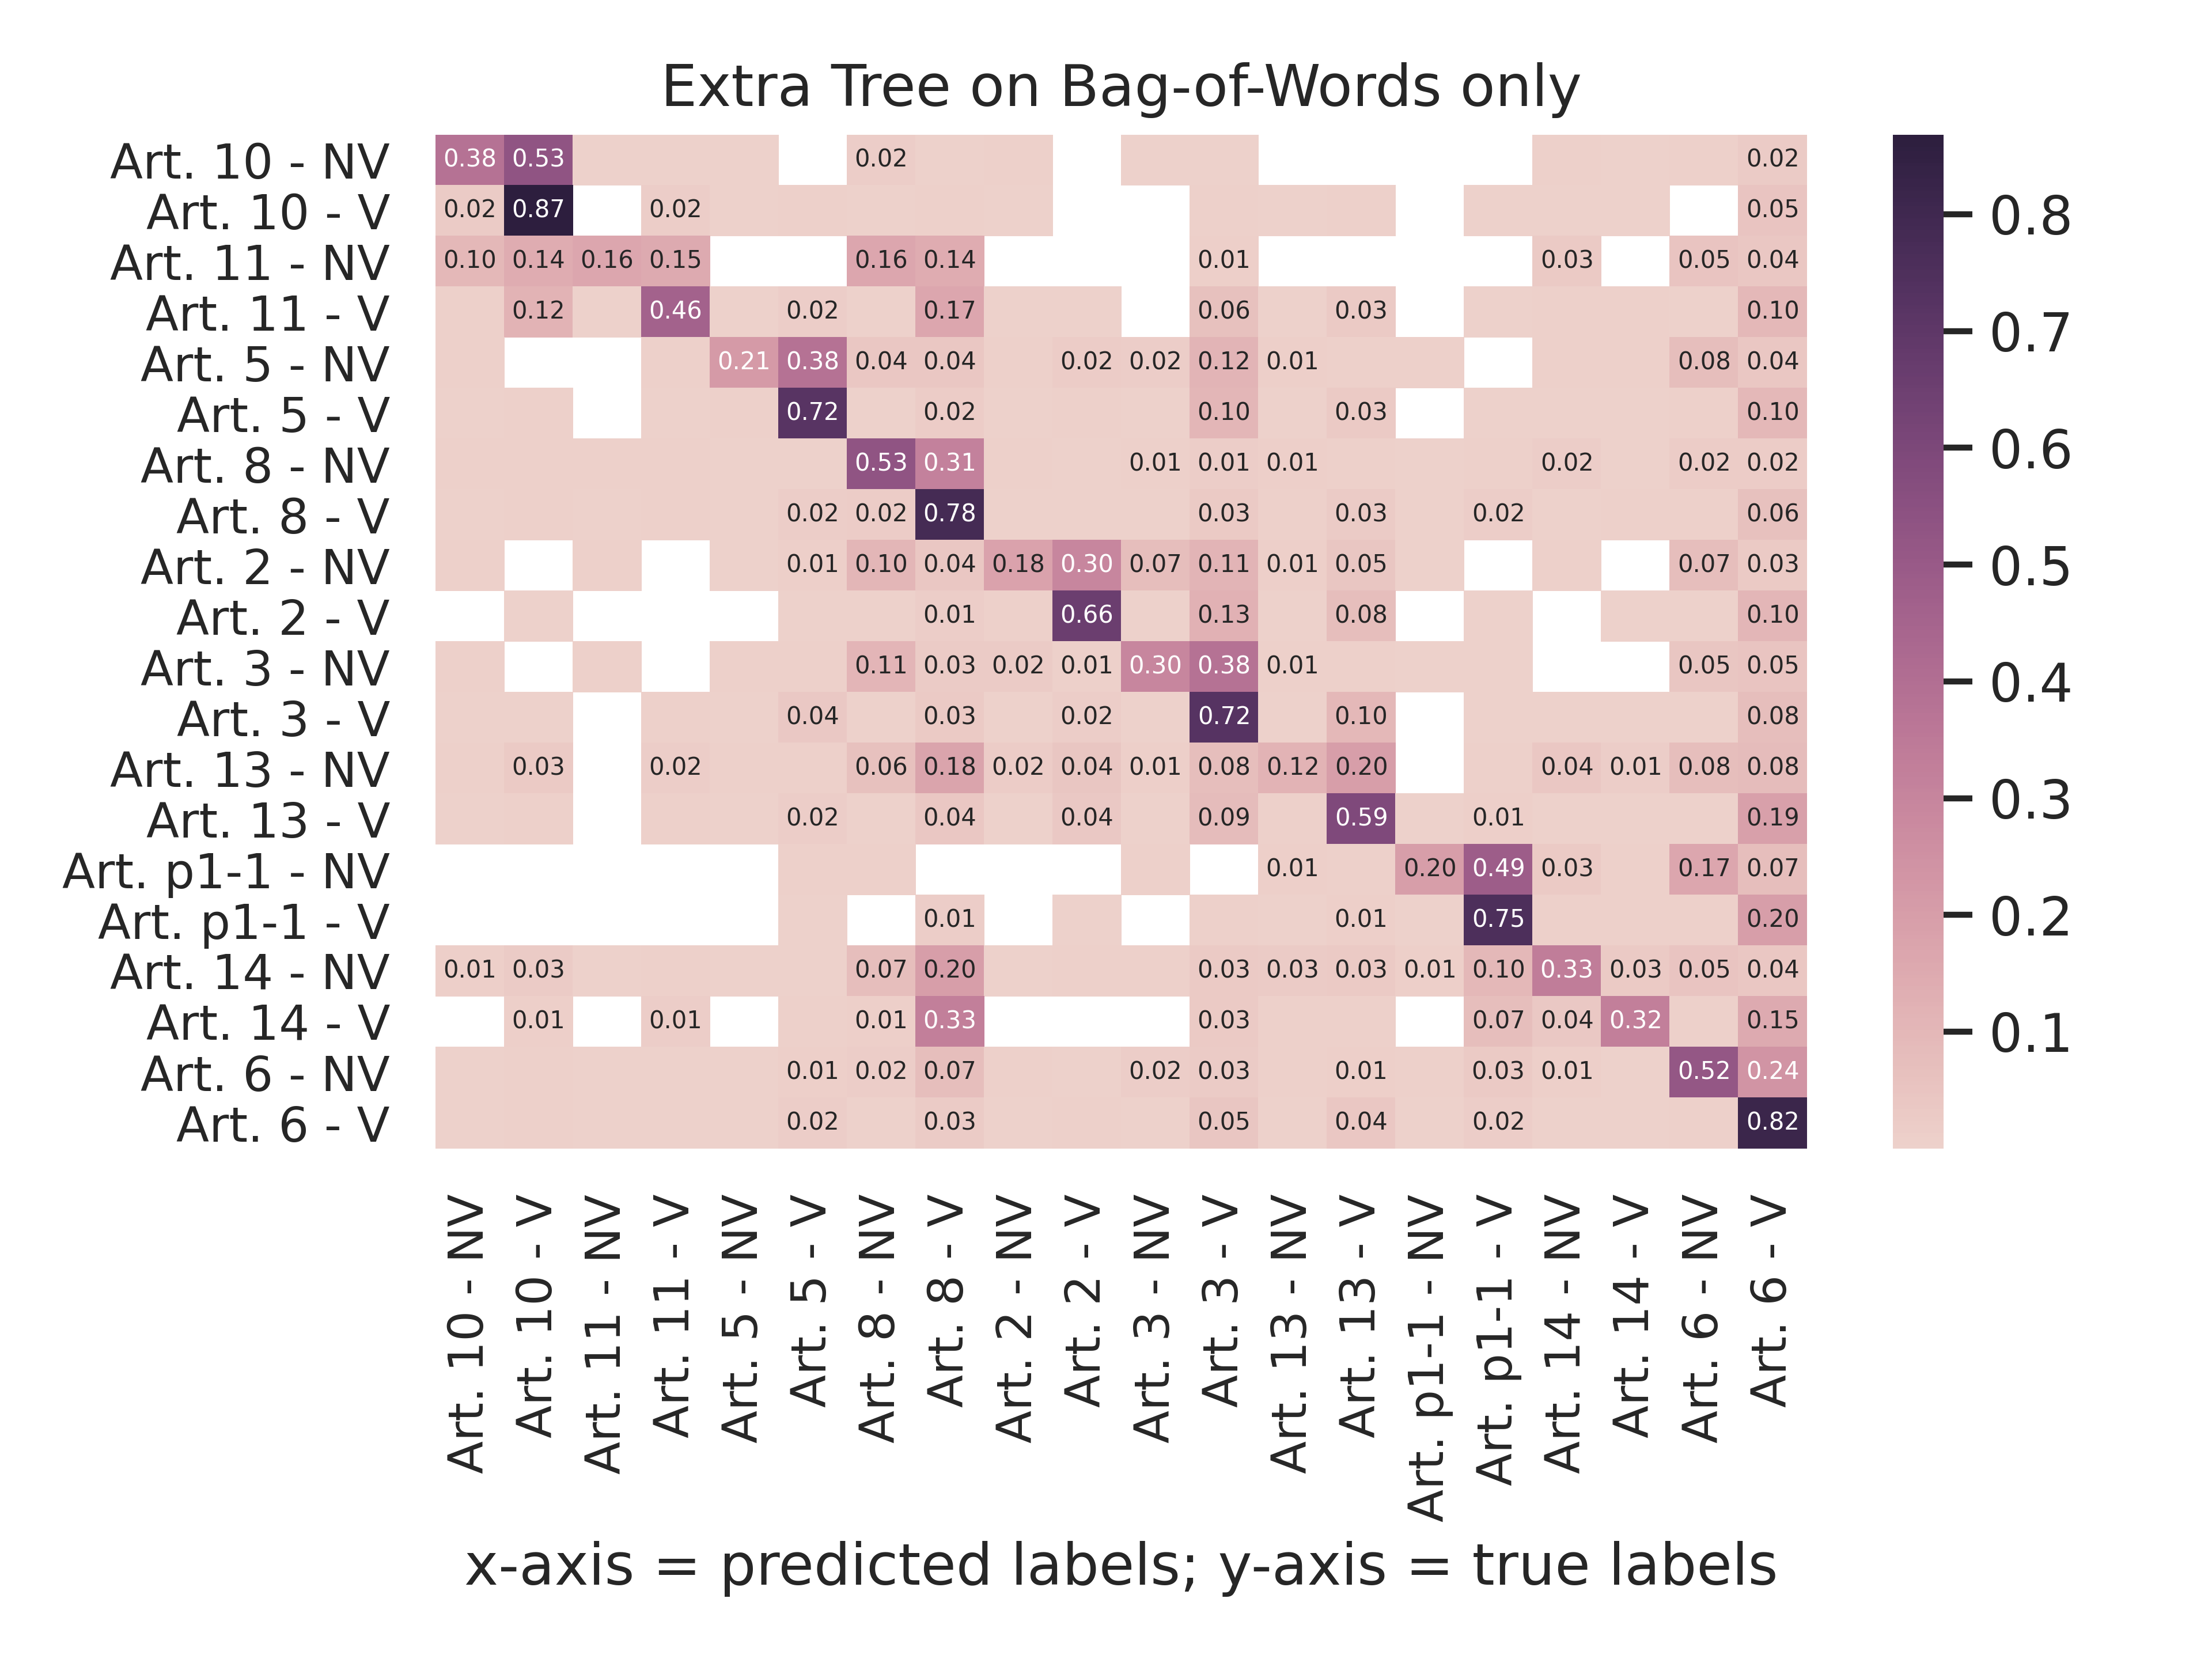
\includegraphics[scale=0.7]{data/analysis/cm/multiclass_cm_test_extra_tree_bag-of-words_only.png}  
\end{figure}
\begin{figure}[!htb]
    \centering
    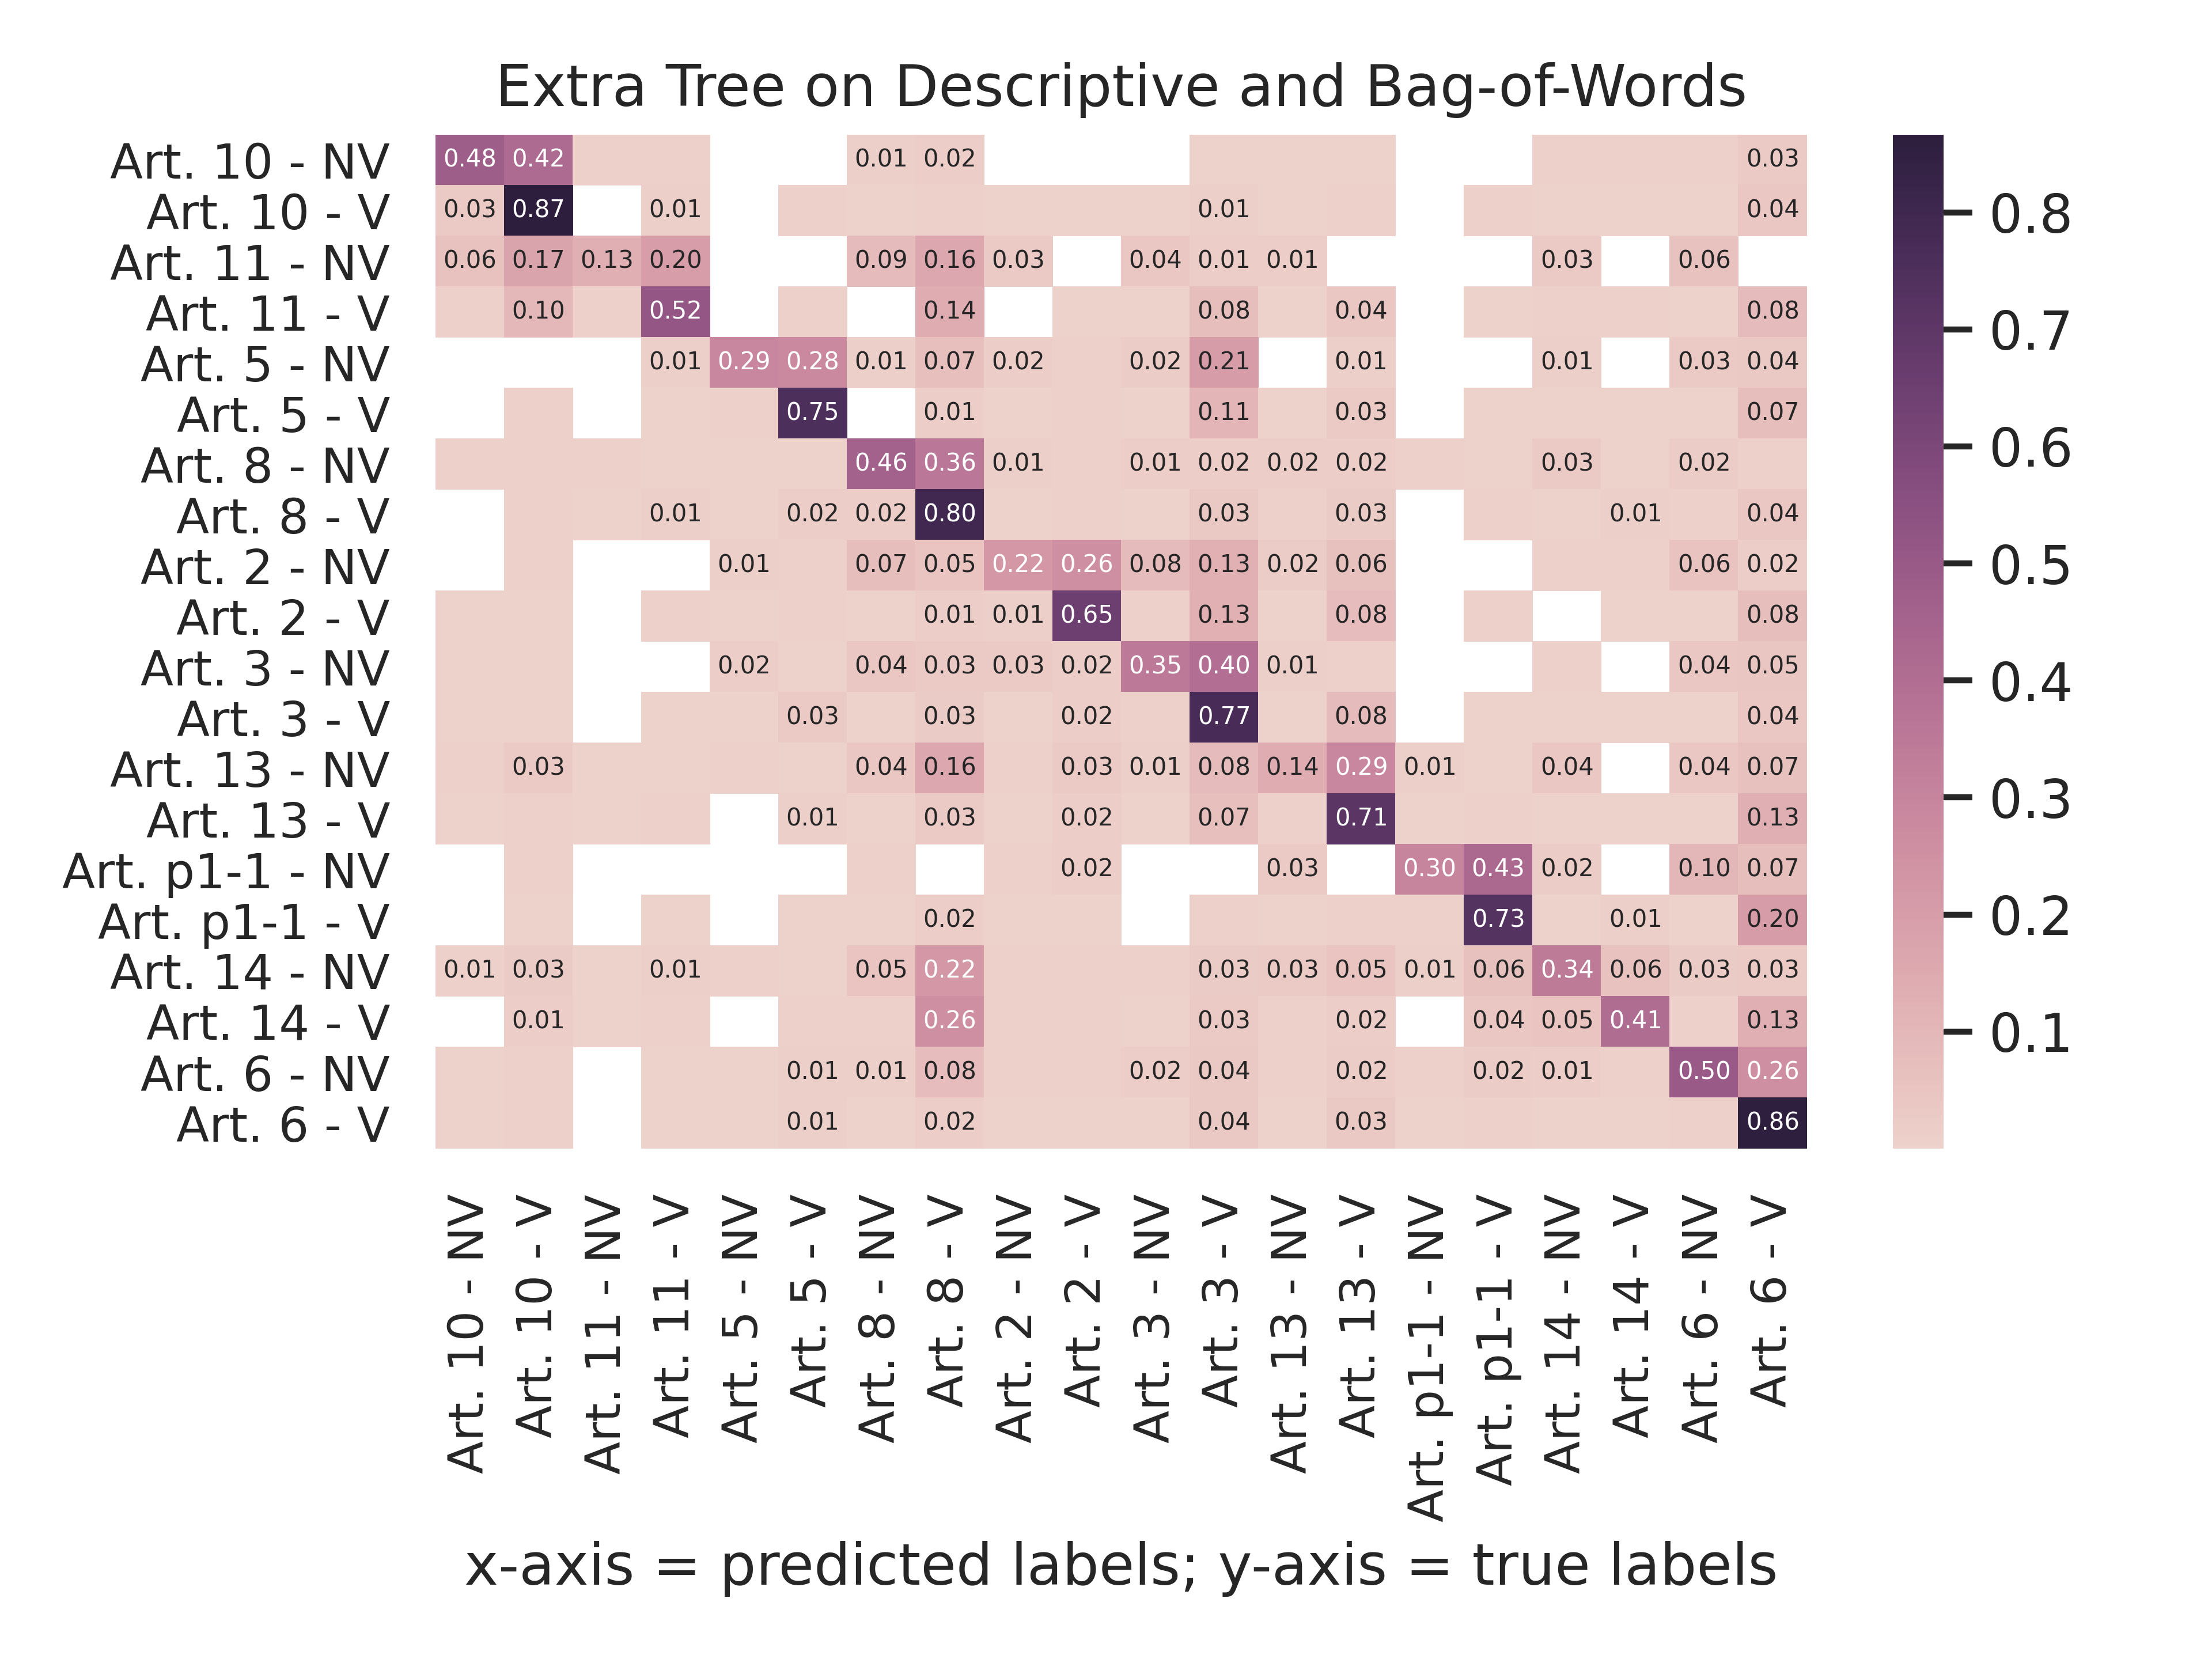
\includegraphics[scale=0.7]{data/analysis/cm/multiclass_cm_test_extra_tree_descriptive_and_bag-of-words.png}  
\end{figure}
\begin{figure}[!htb]
    \centering
    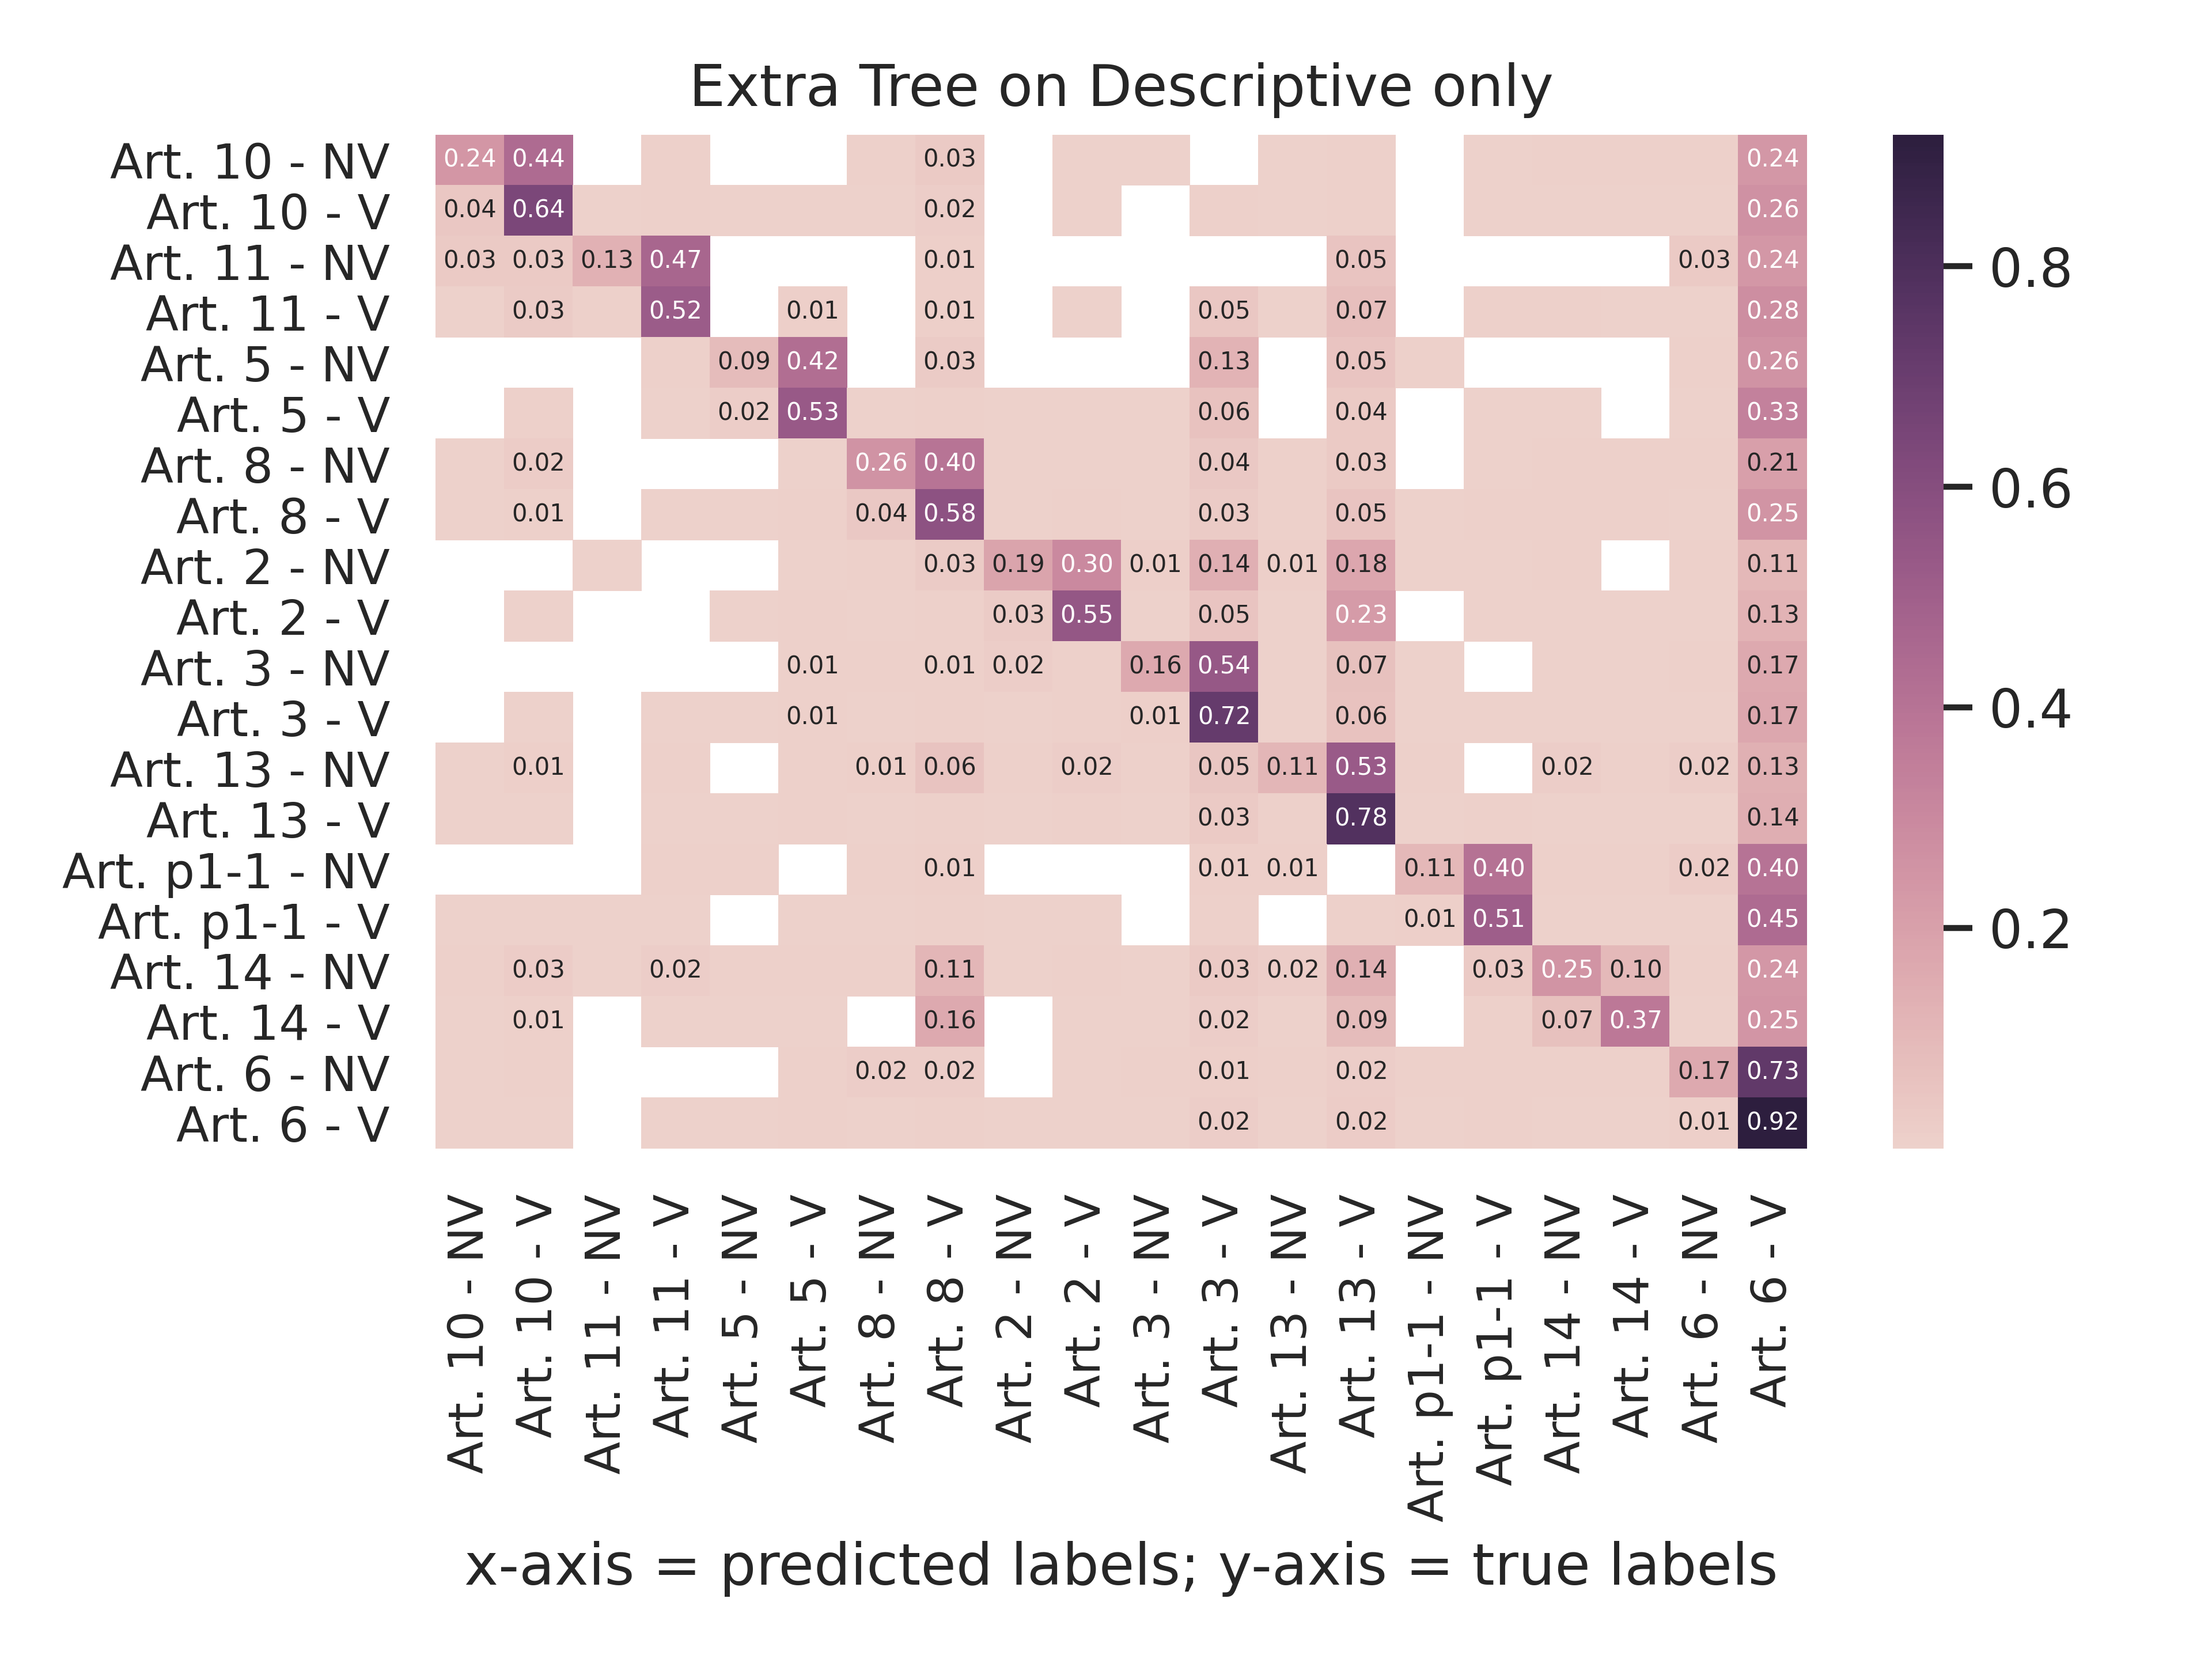
\includegraphics[scale=0.7]{data/analysis/cm/multiclass_cm_test_extra_tree_descriptive_only.png}  
\end{figure}
\begin{figure}[!htb]
    \centering
    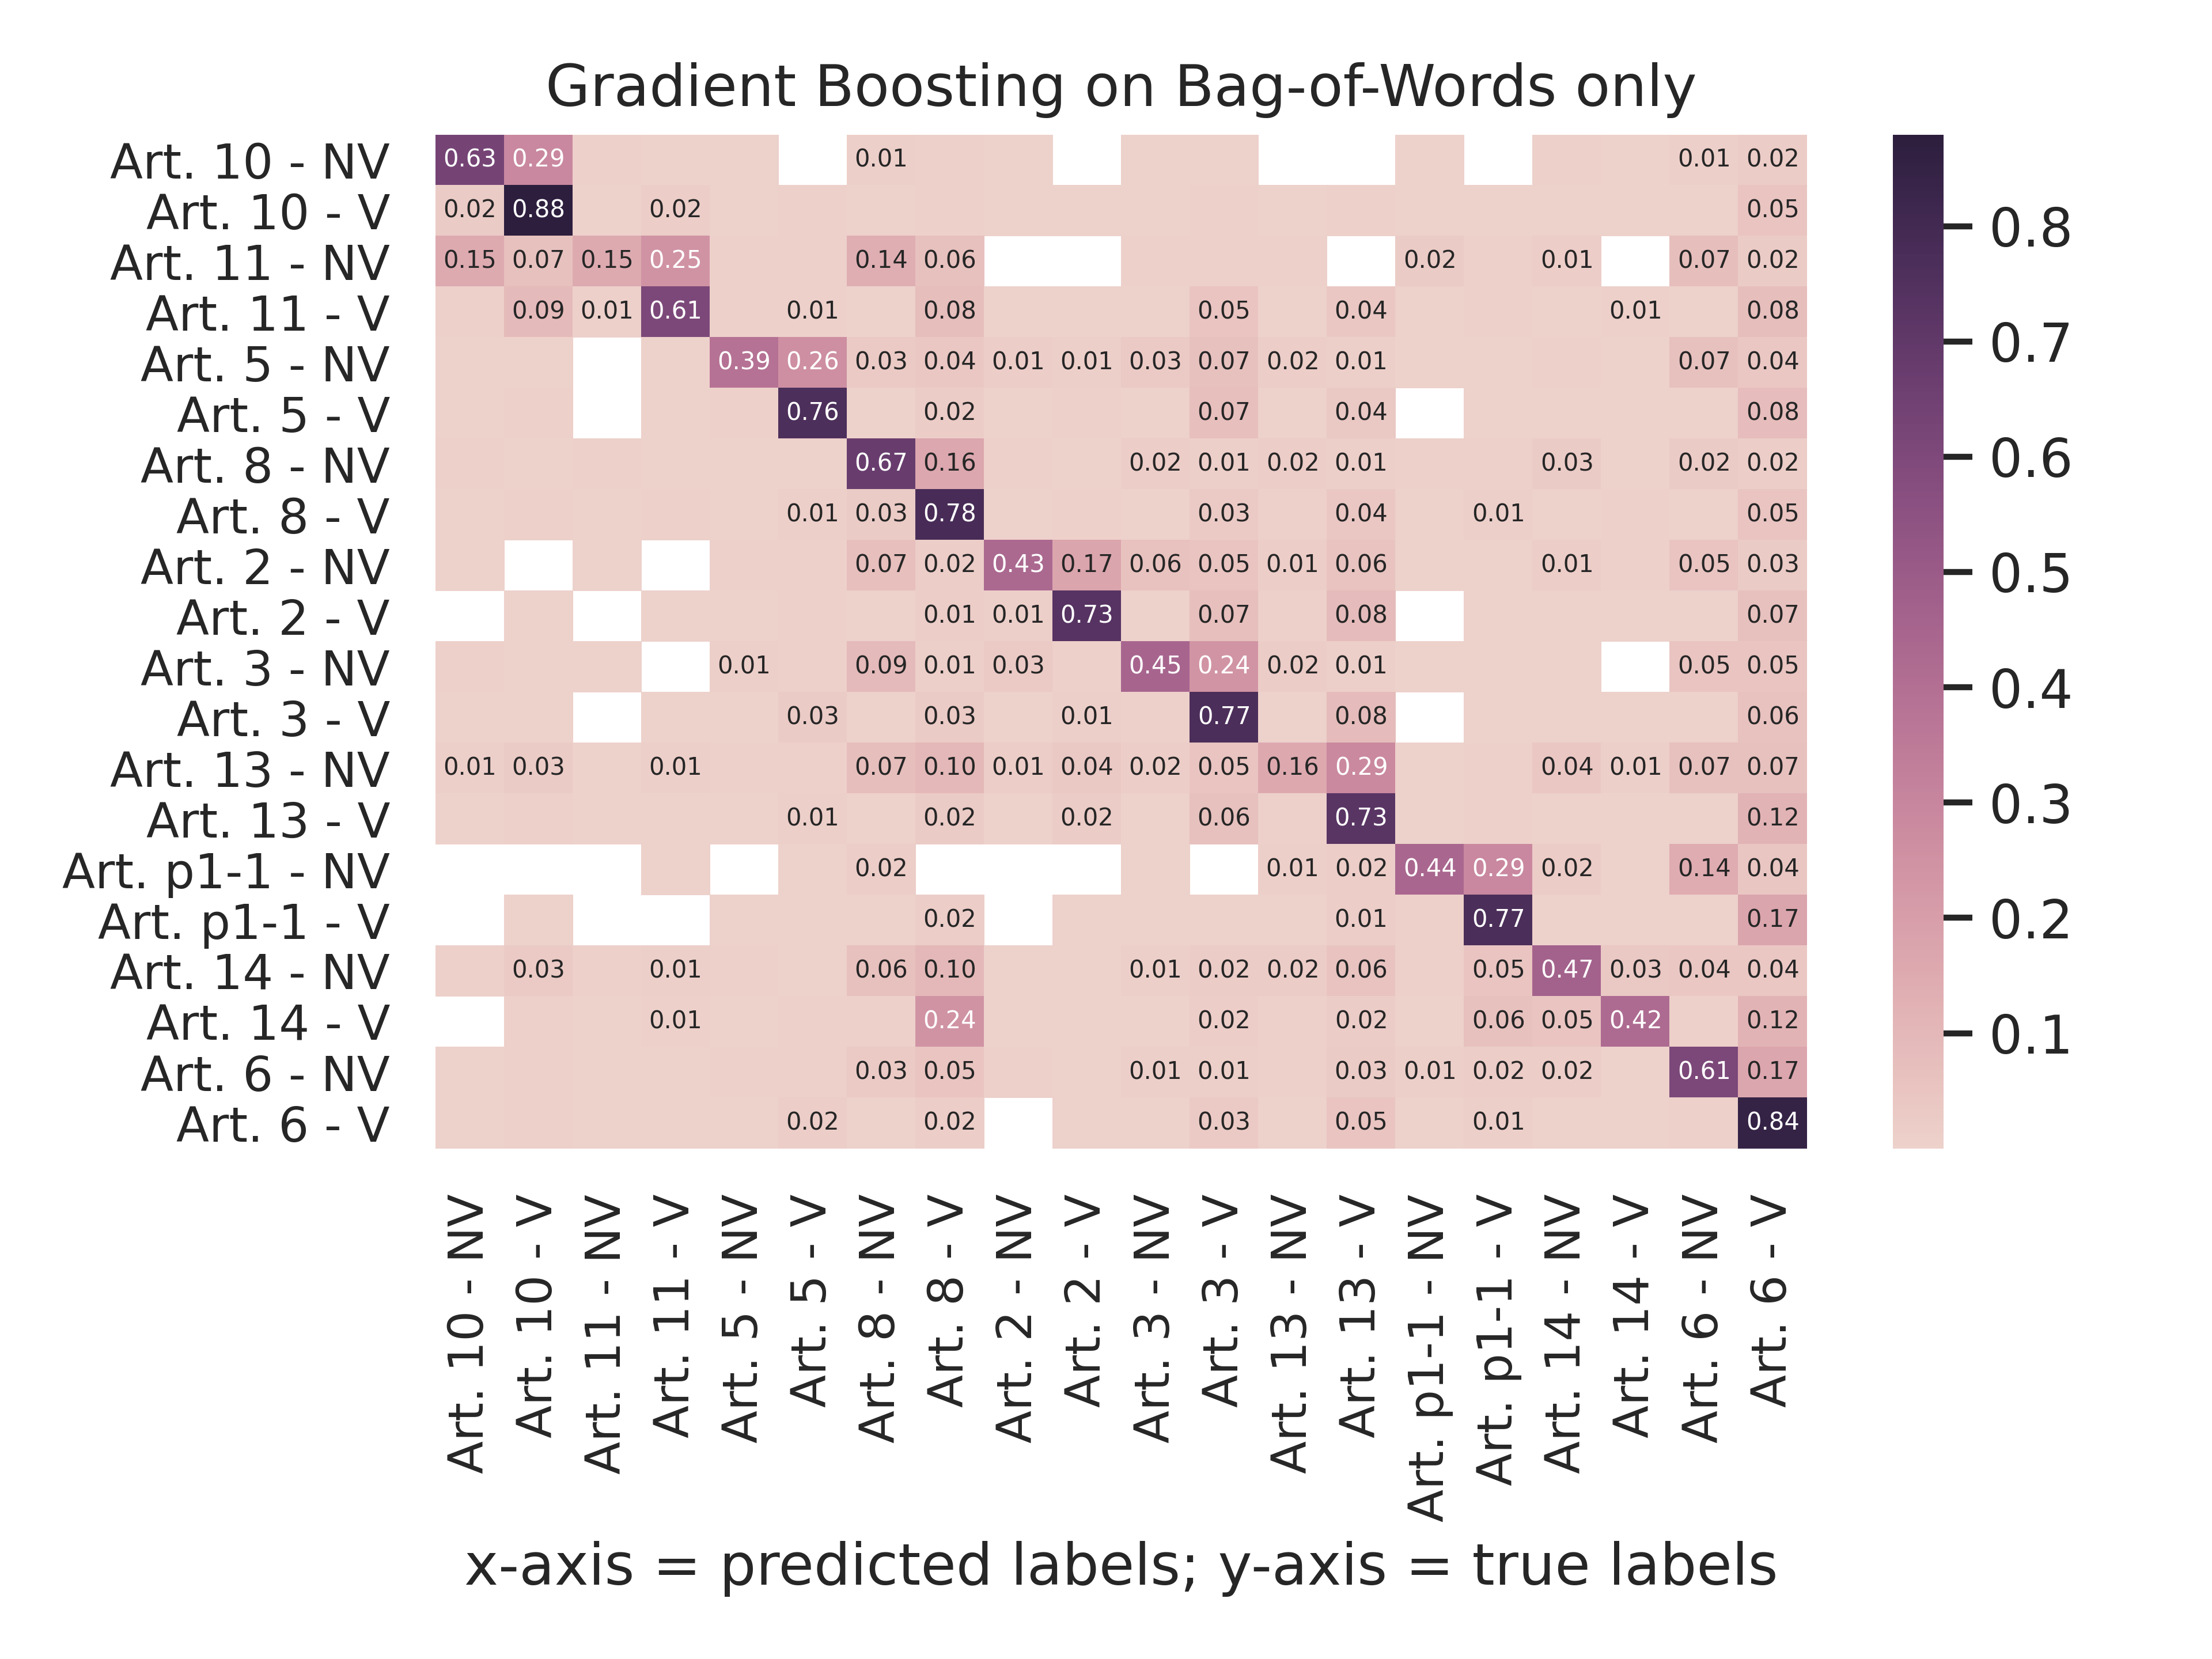
\includegraphics[scale=0.7]{data/analysis/cm/multiclass_cm_test_gradient_boosting_bag-of-words_only.png}  
\end{figure}
\begin{figure}[!htb]
    \centering
    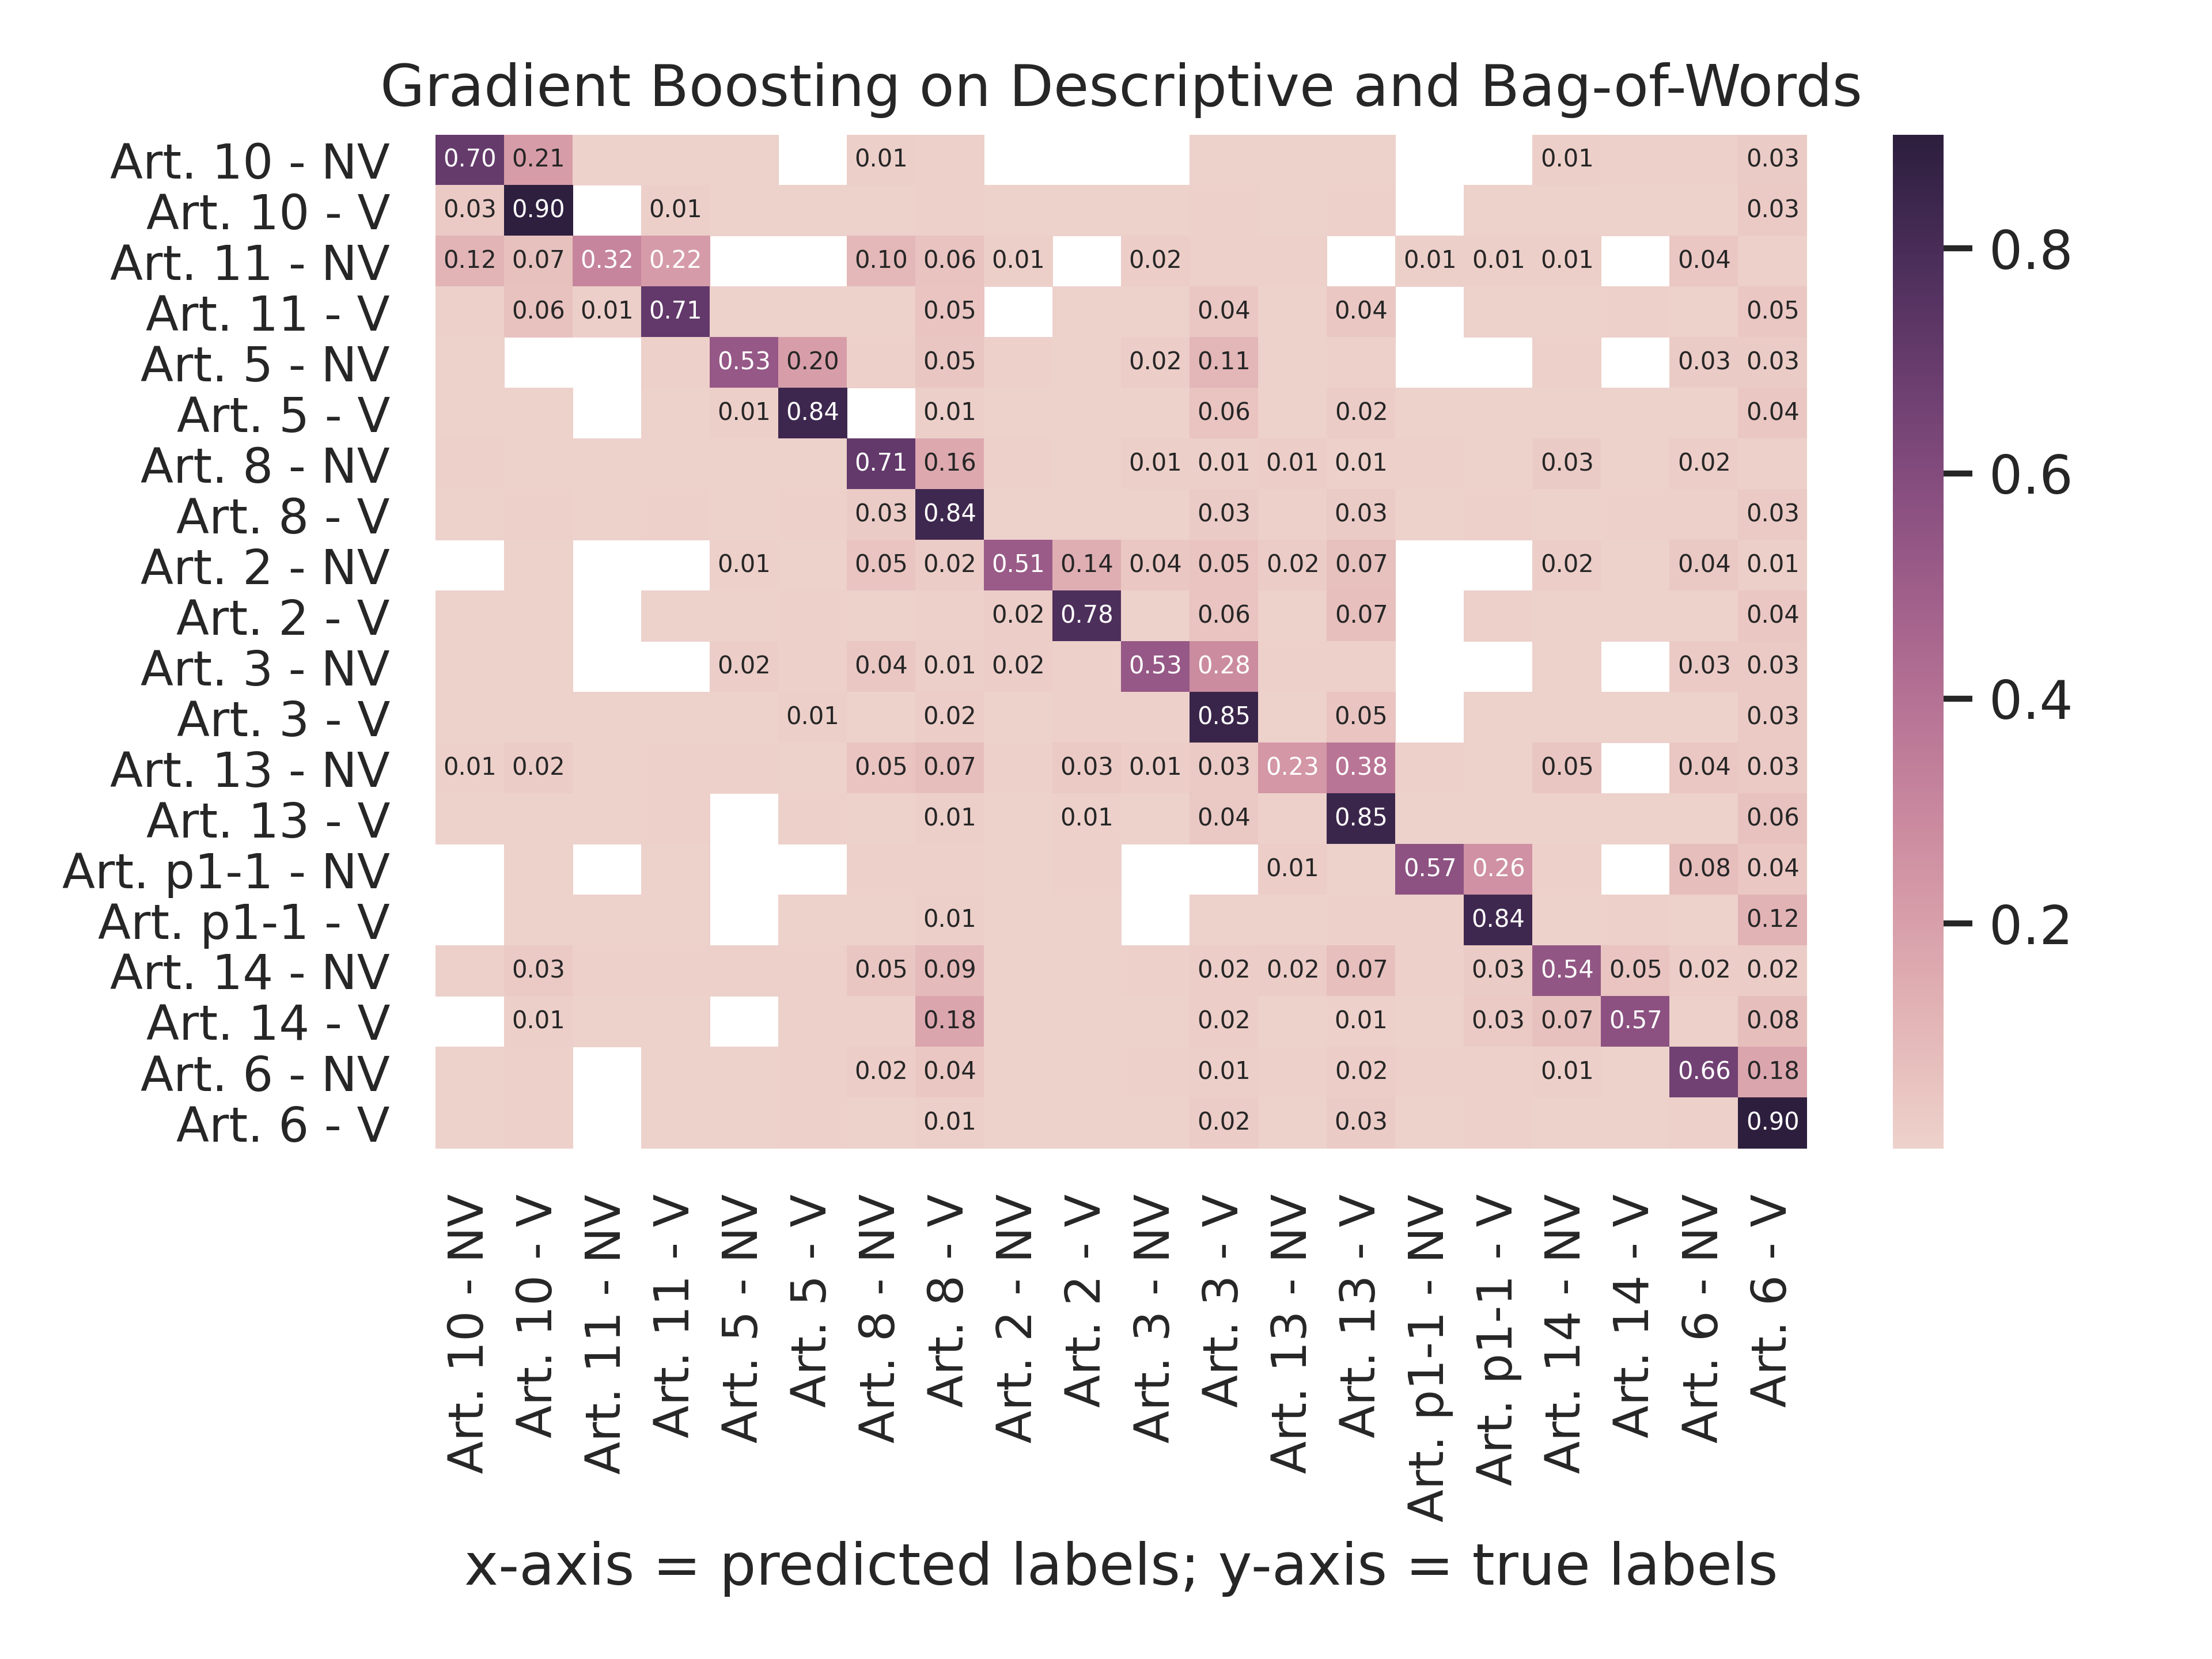
\includegraphics[scale=0.7]{data/analysis/cm/multiclass_cm_test_gradient_boosting_descriptive_and_bag-of-words.png}  
\end{figure}
\begin{figure}[!htb]
    \centering
    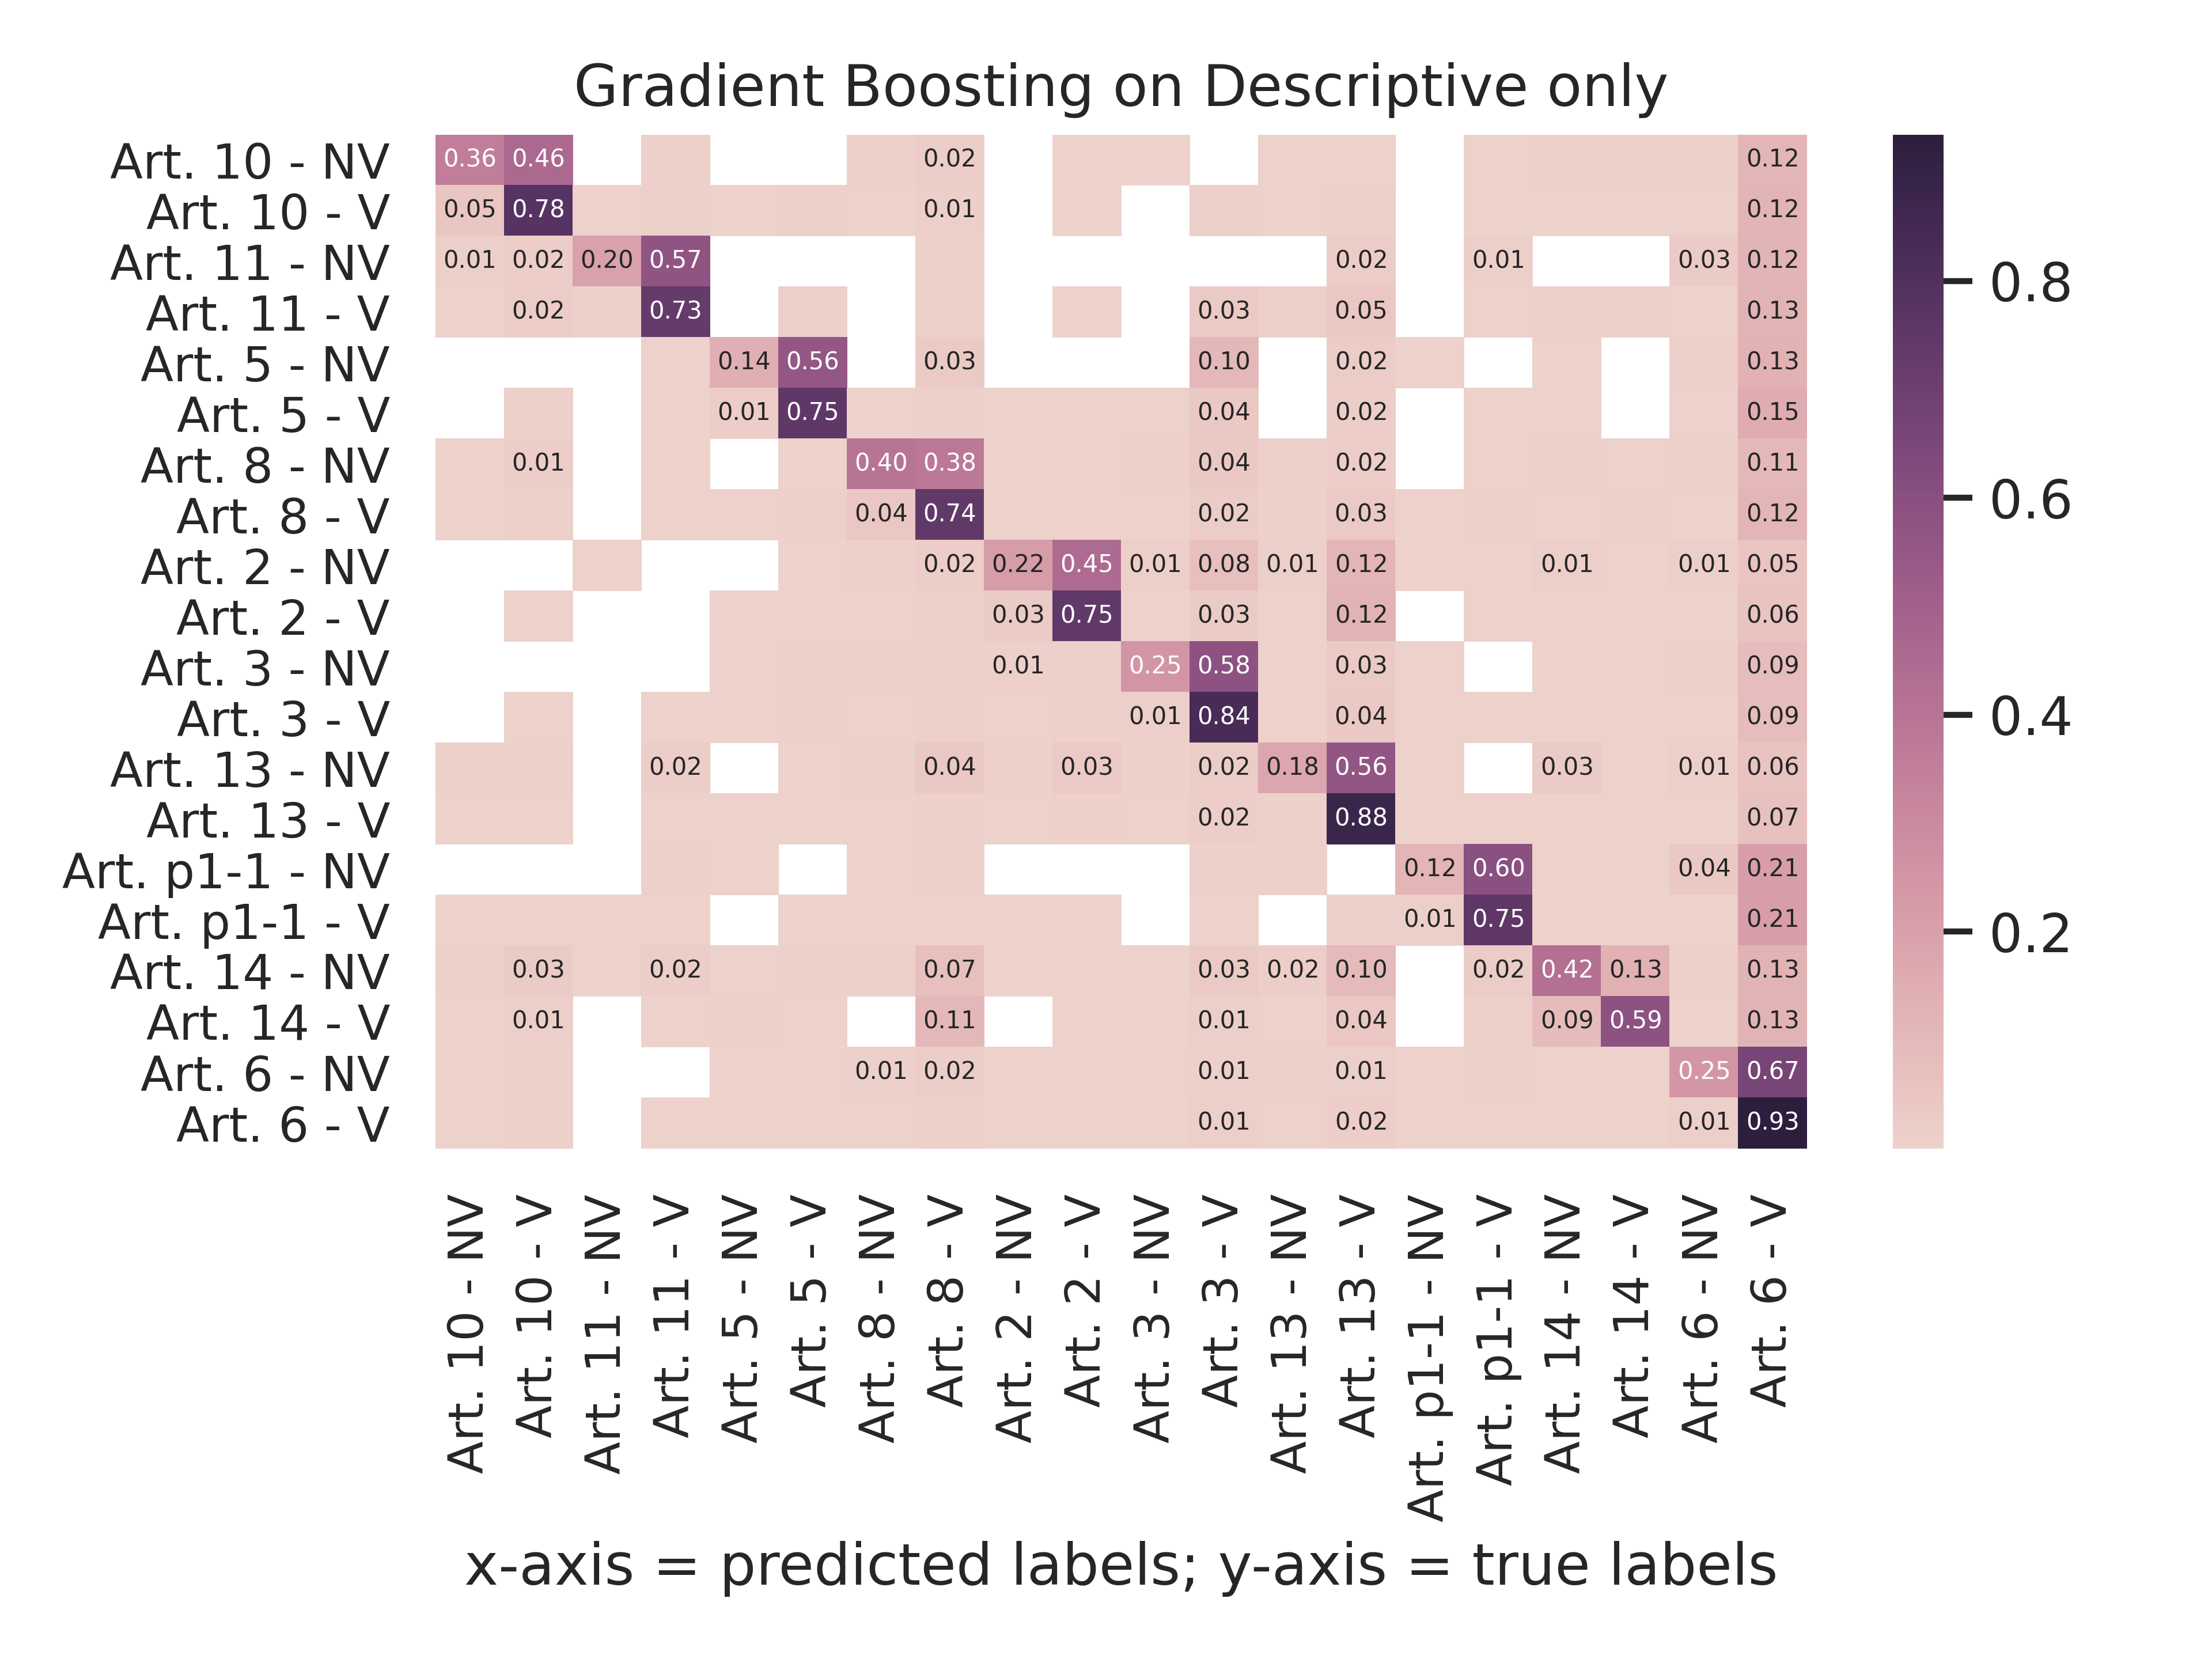
\includegraphics[scale=0.7]{data/analysis/cm/multiclass_cm_test_gradient_boosting_descriptive_only.png}  
\end{figure}
\begin{figure}[!htb]
    \centering
    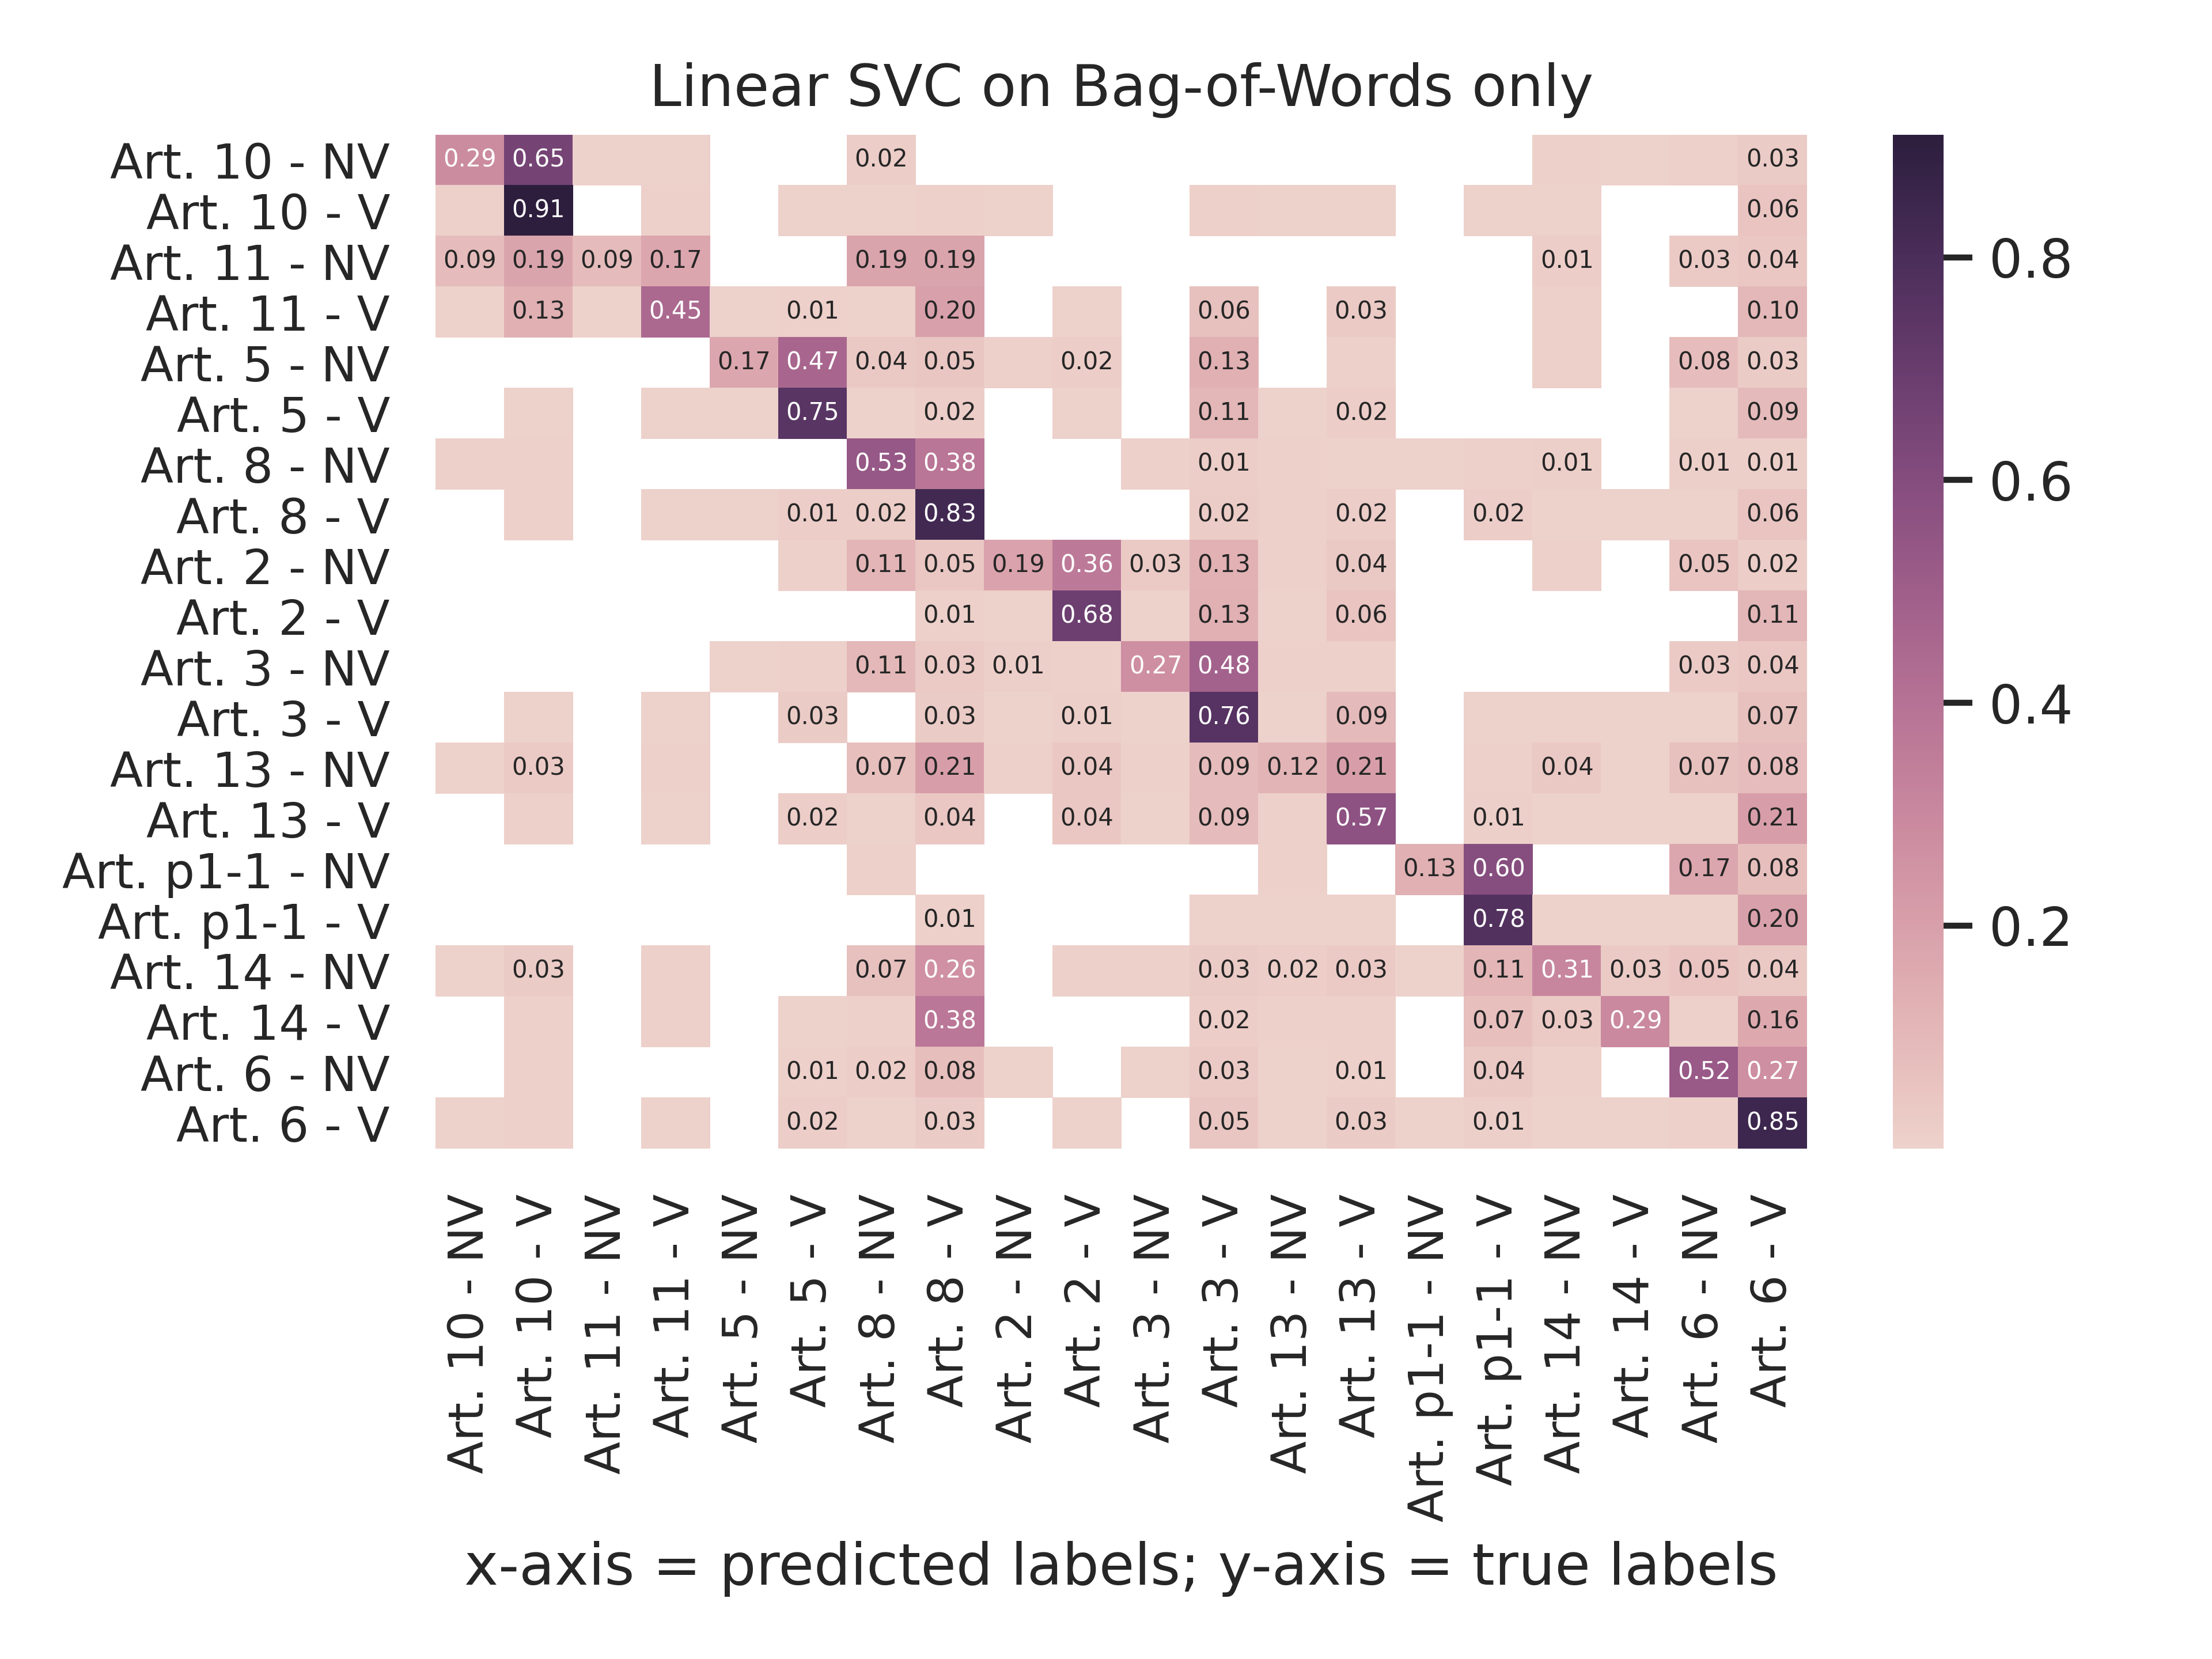
\includegraphics[scale=0.7]{data/analysis/cm/multiclass_cm_test_linear_svc_bag-of-words_only.png}  
\end{figure}
\begin{figure}[!htb]
    \centering
    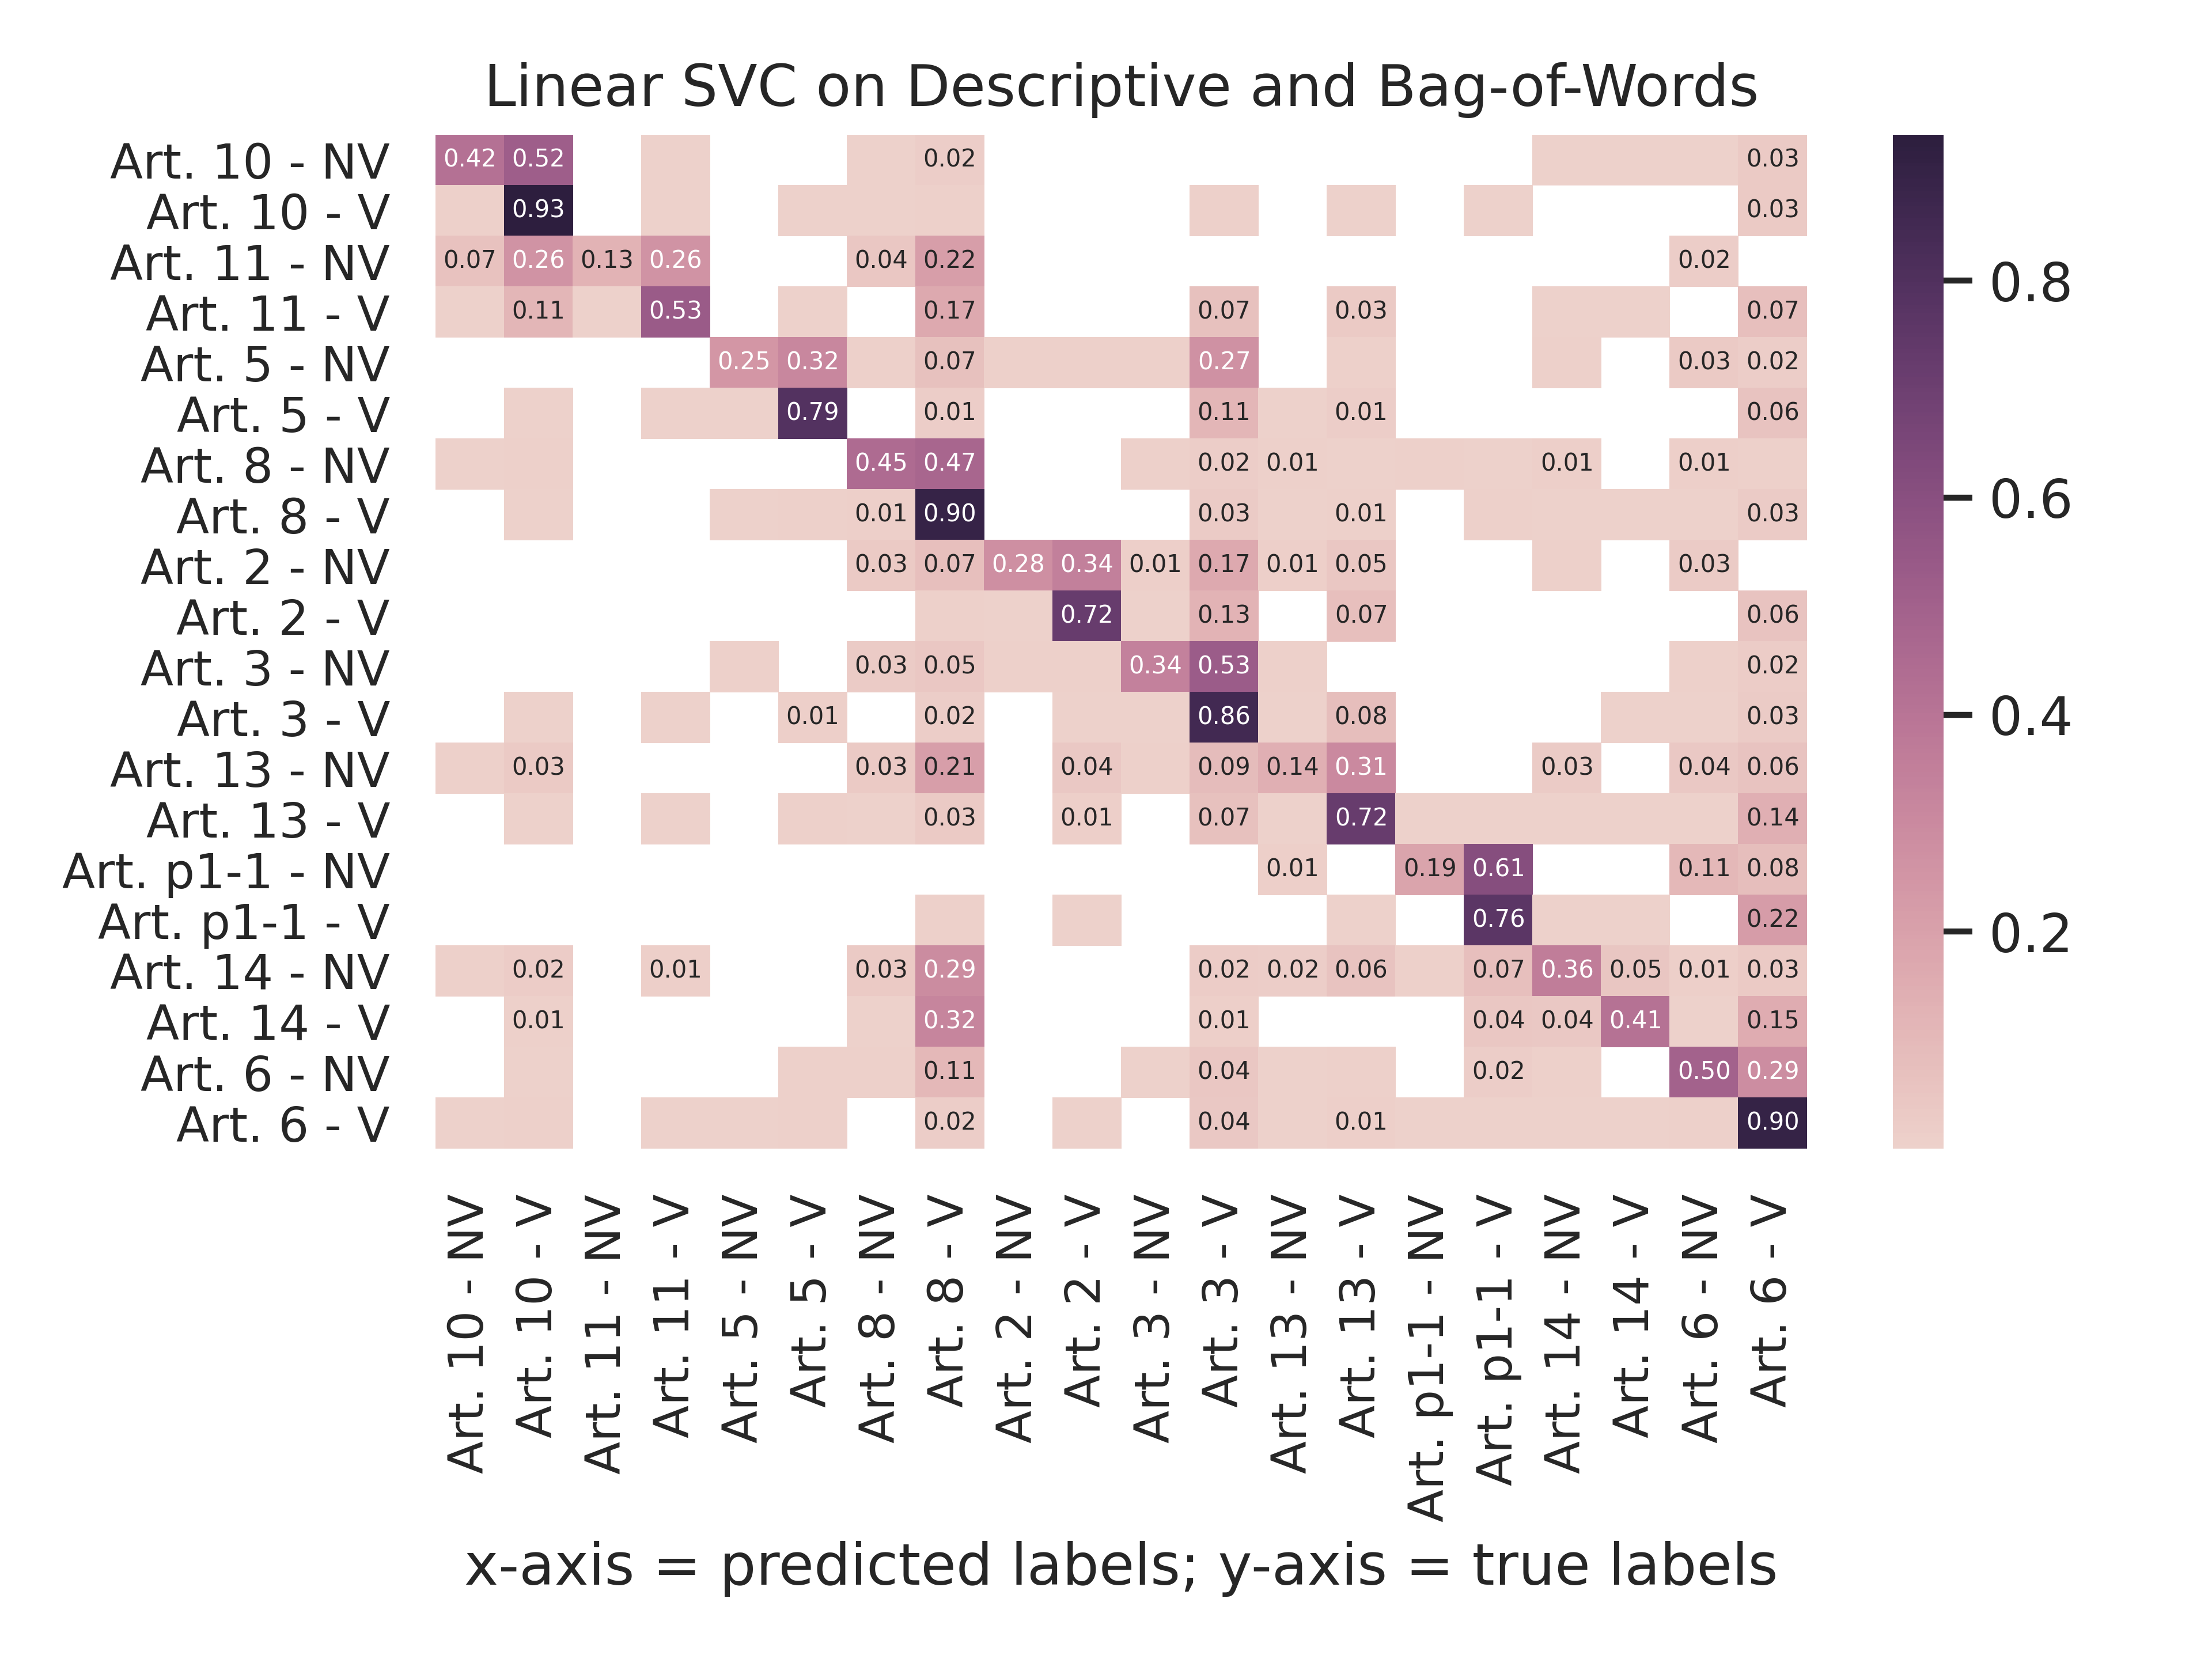
\includegraphics[scale=0.7]{data/analysis/cm/multiclass_cm_test_linear_svc_descriptive_and_bag-of-words.png}  
\end{figure}
\begin{figure}[!htb]
    \centering
    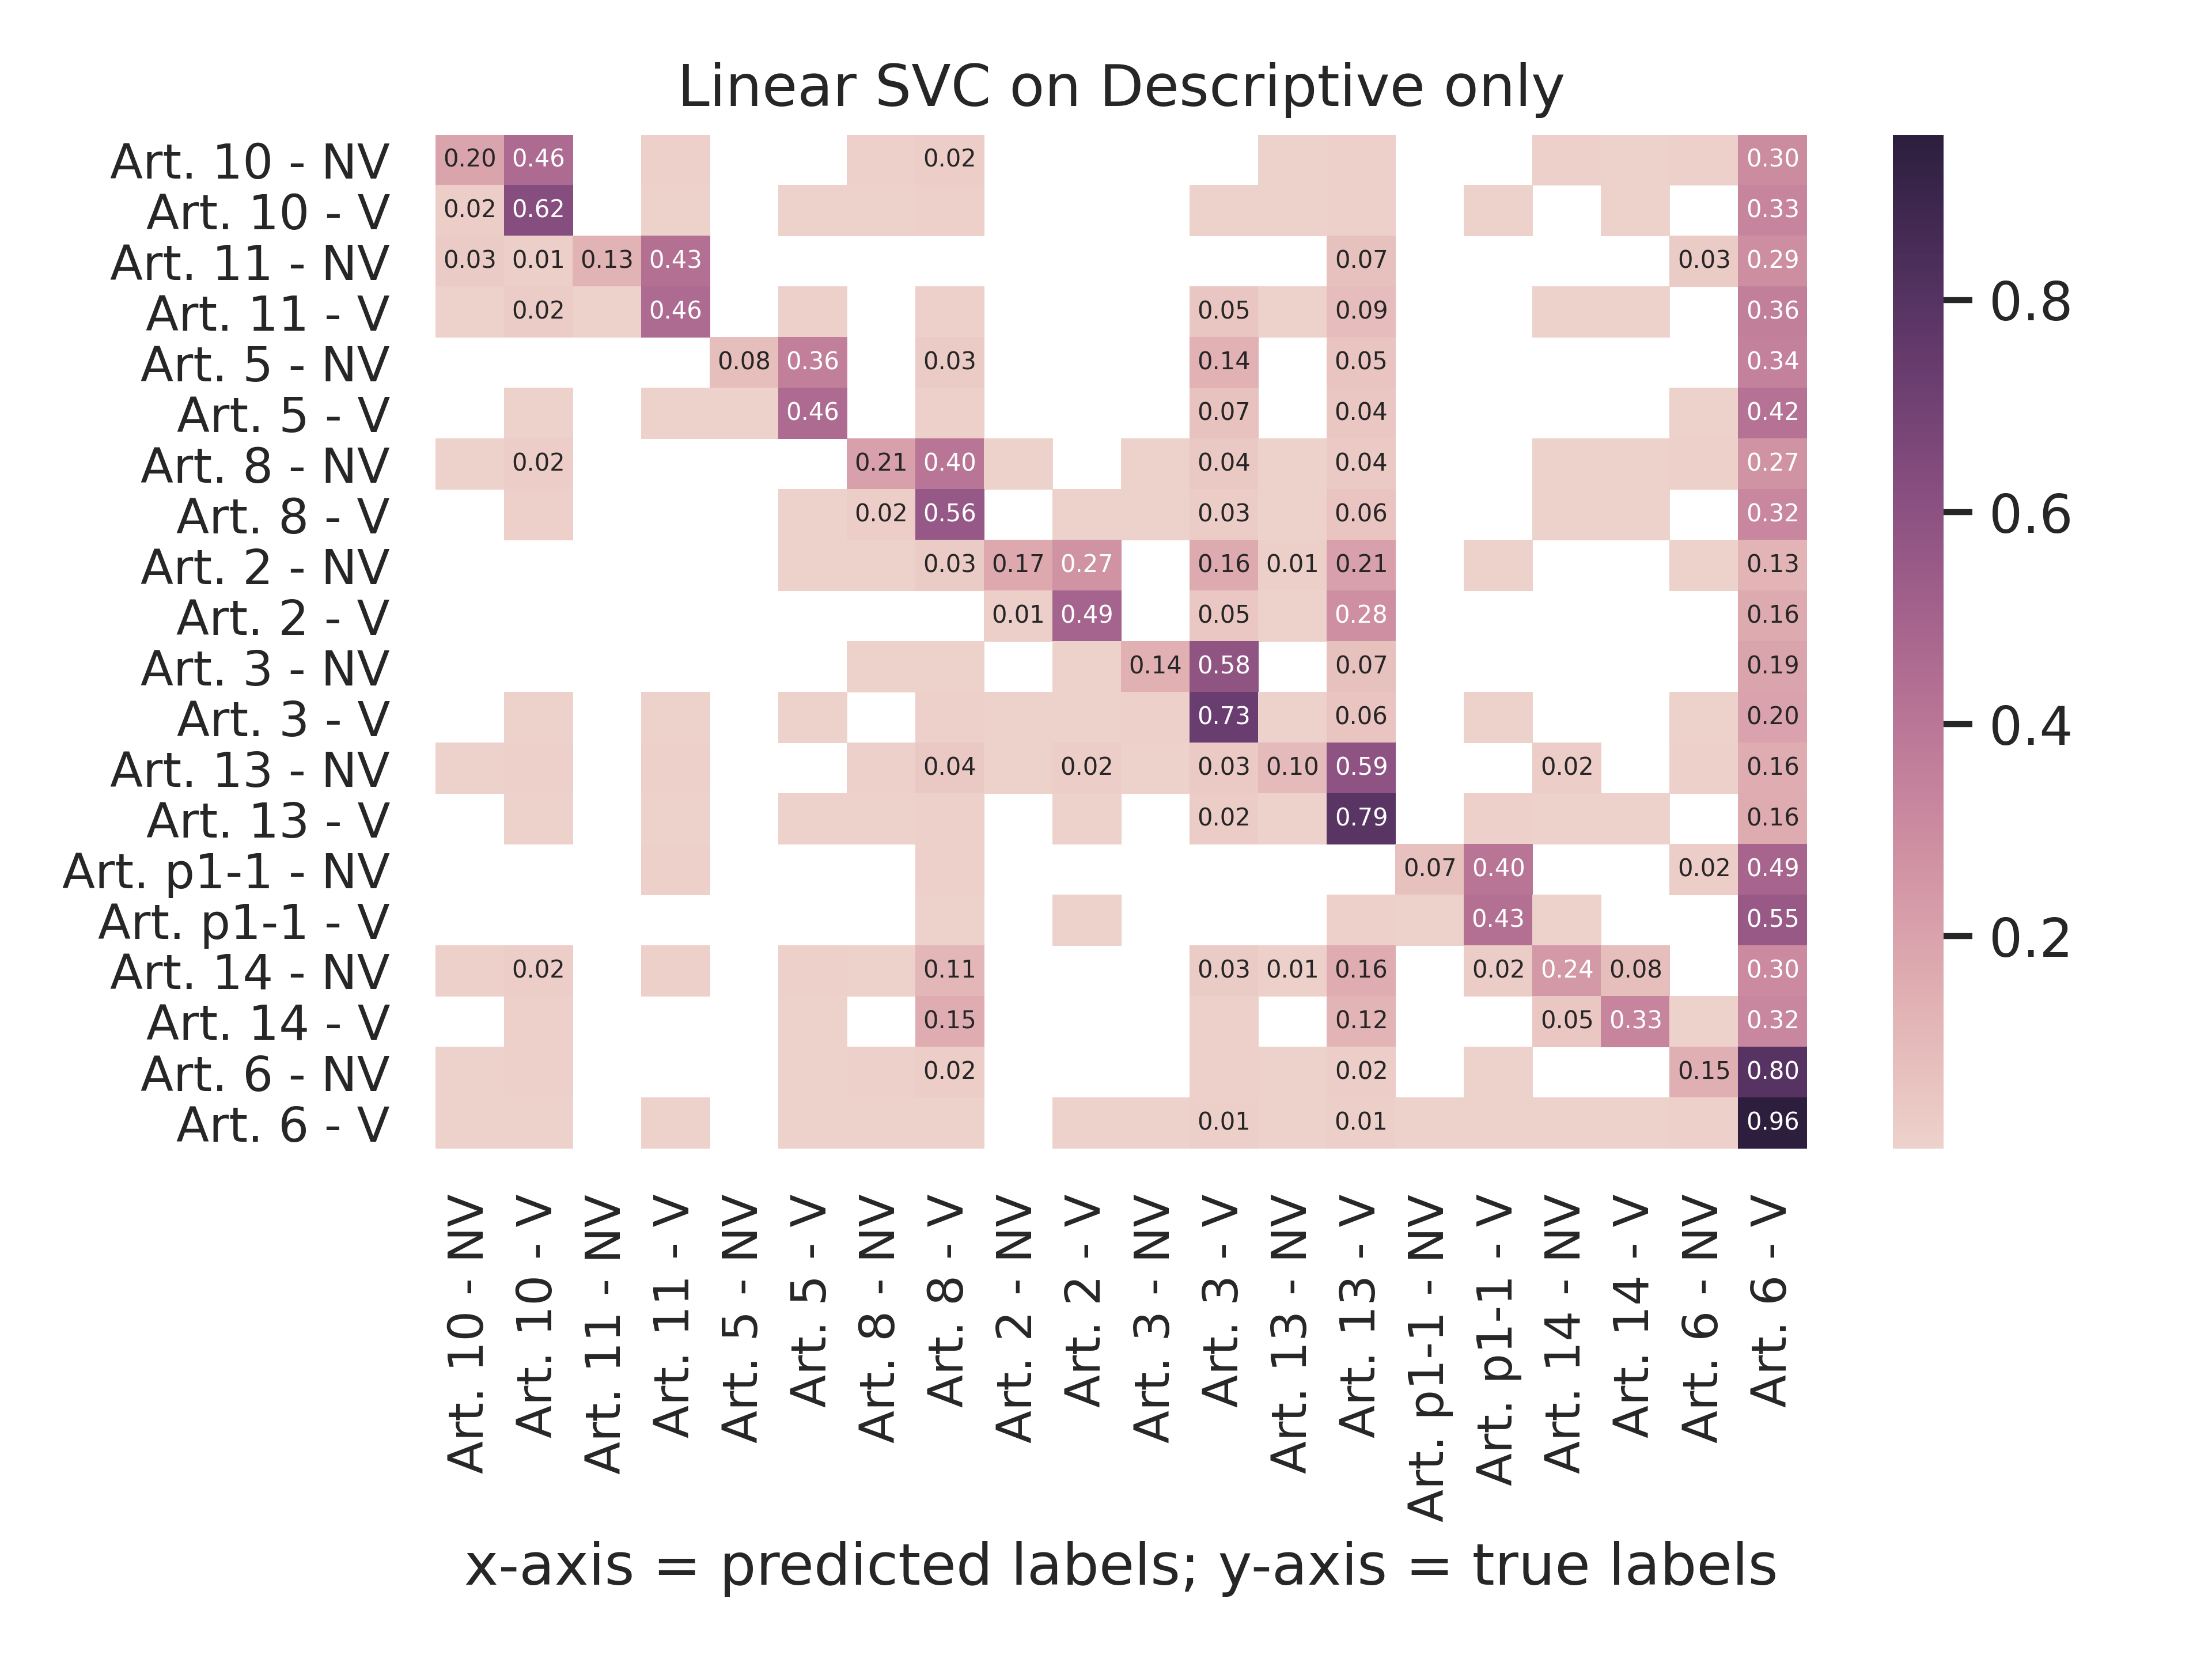
\includegraphics[scale=0.7]{data/analysis/cm/multiclass_cm_test_linear_svc_descriptive_only.png}  
\end{figure}
\begin{figure}[!htb]
    \centering
    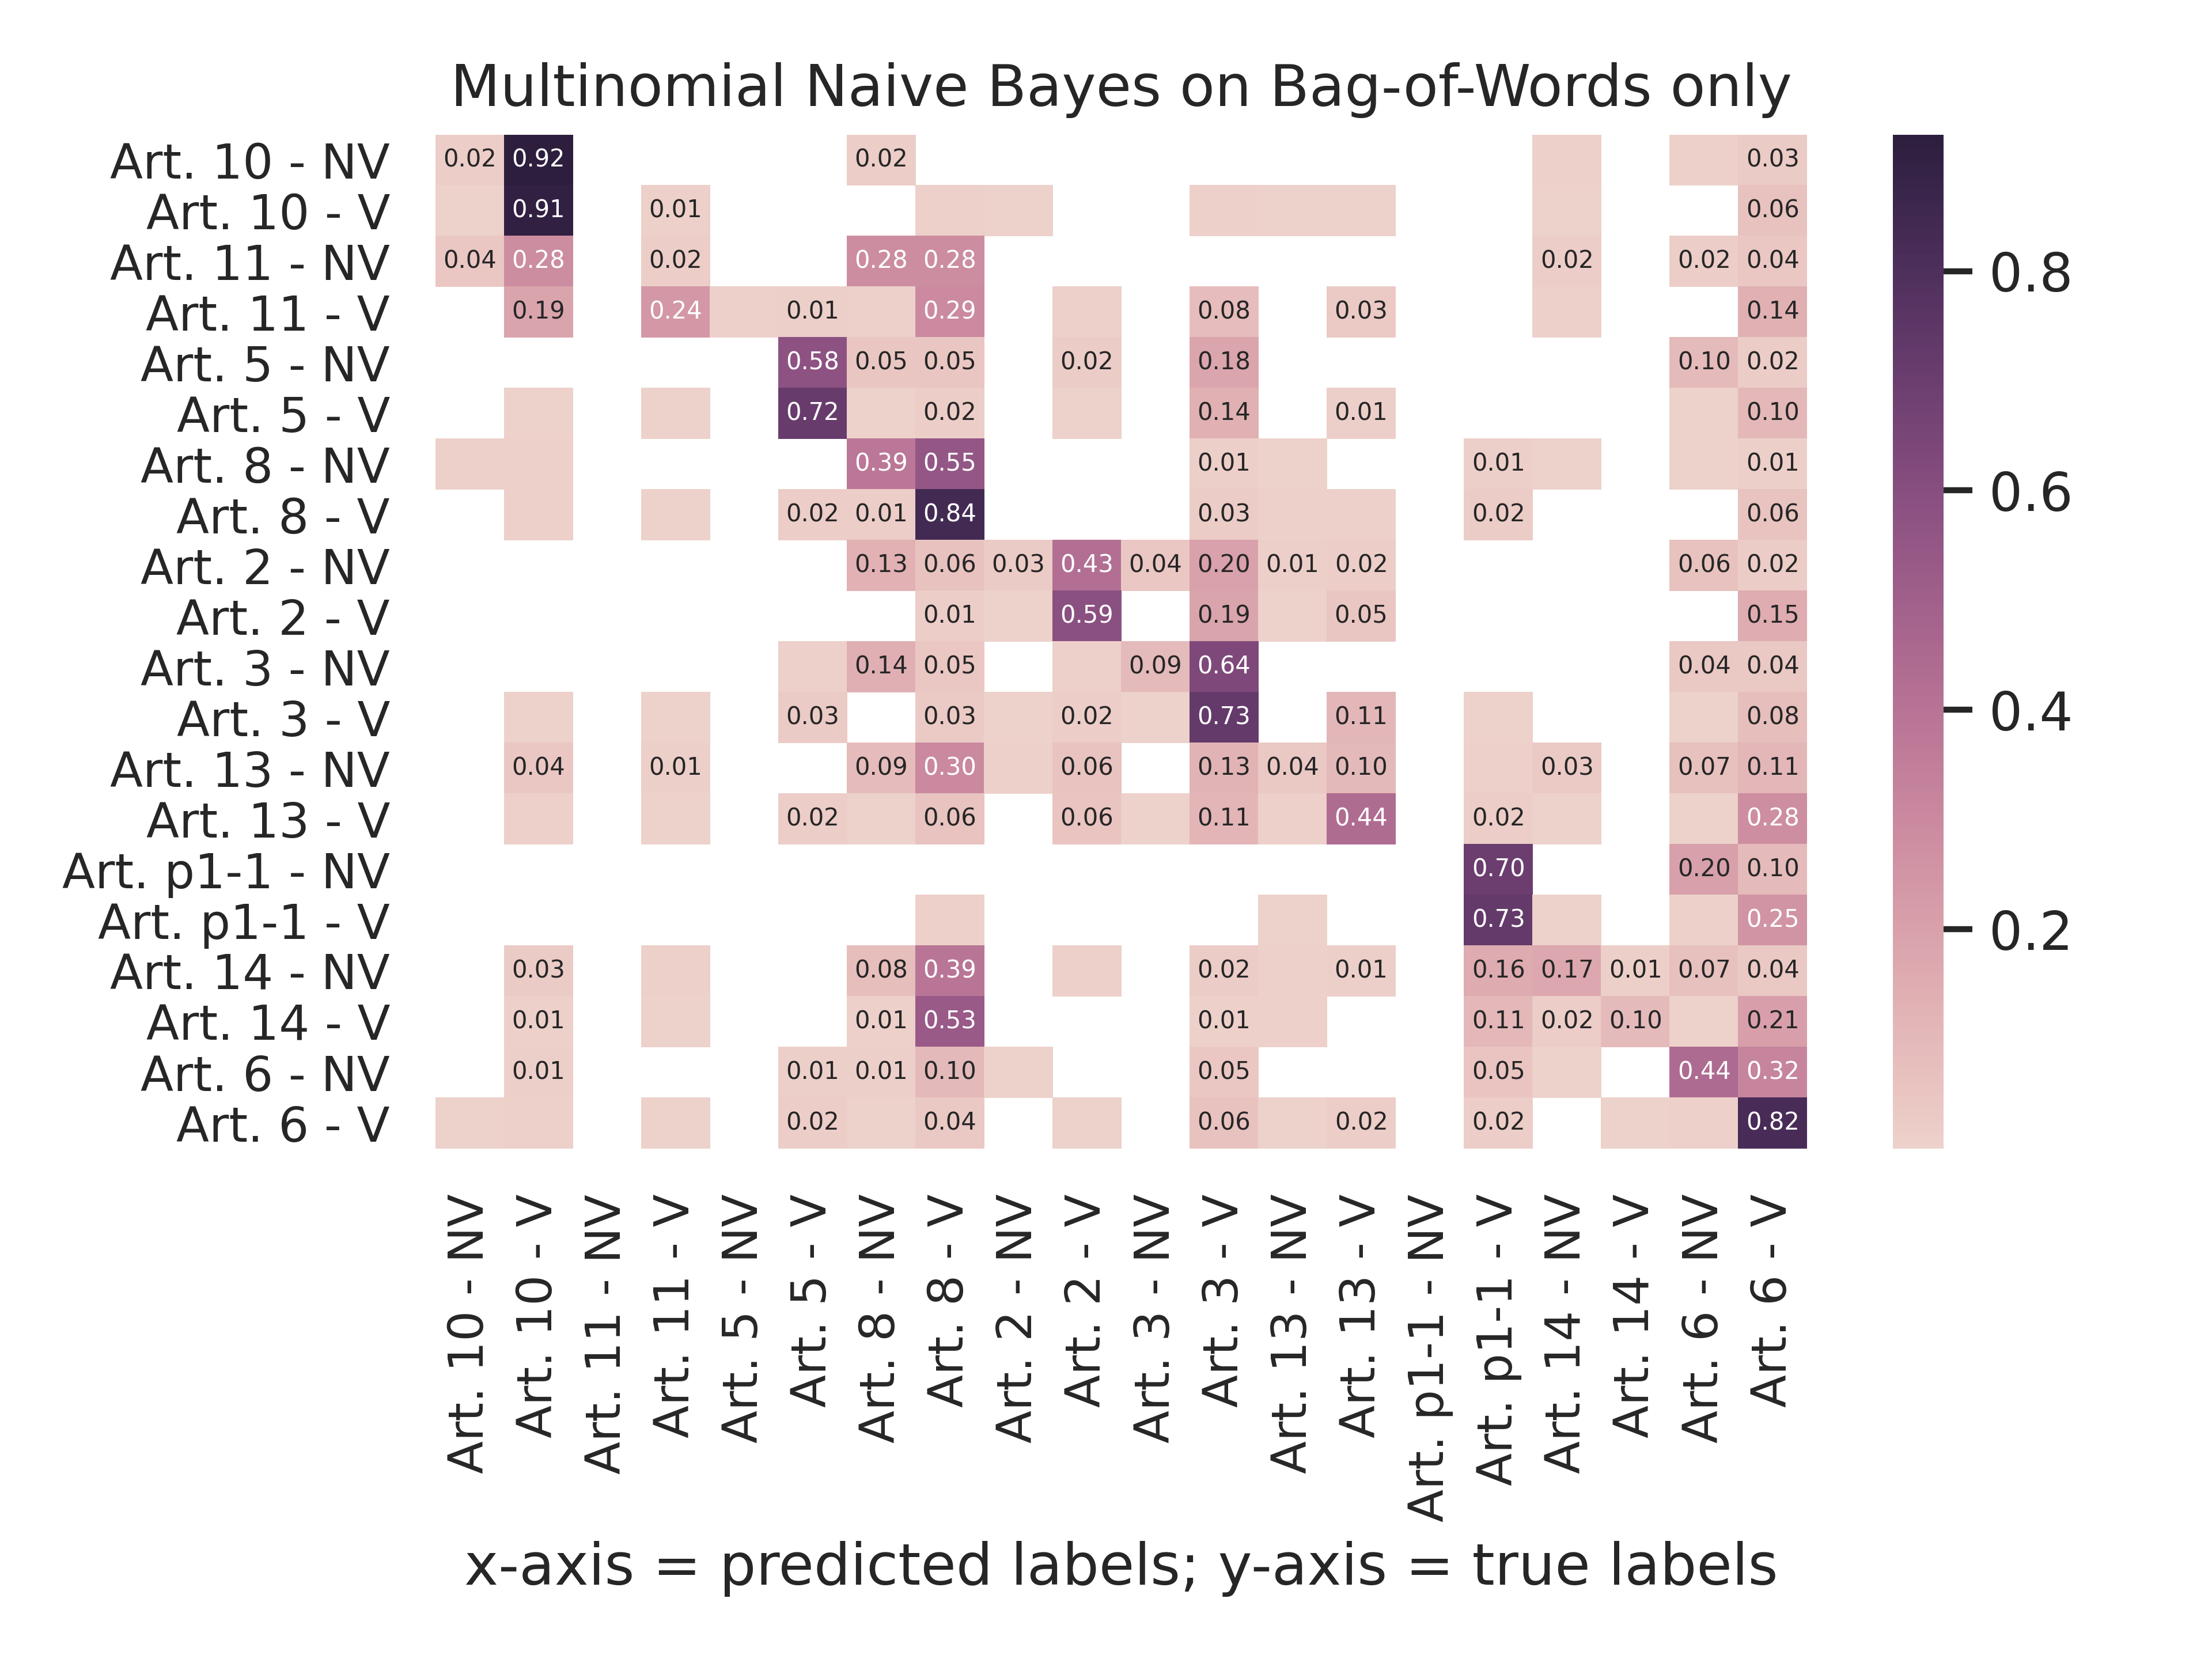
\includegraphics[scale=0.7]{data/analysis/cm/multiclass_cm_test_multinomial_naive_bayes_bag-of-words_only.png}  
\end{figure}
\begin{figure}[!htb]
    \centering
    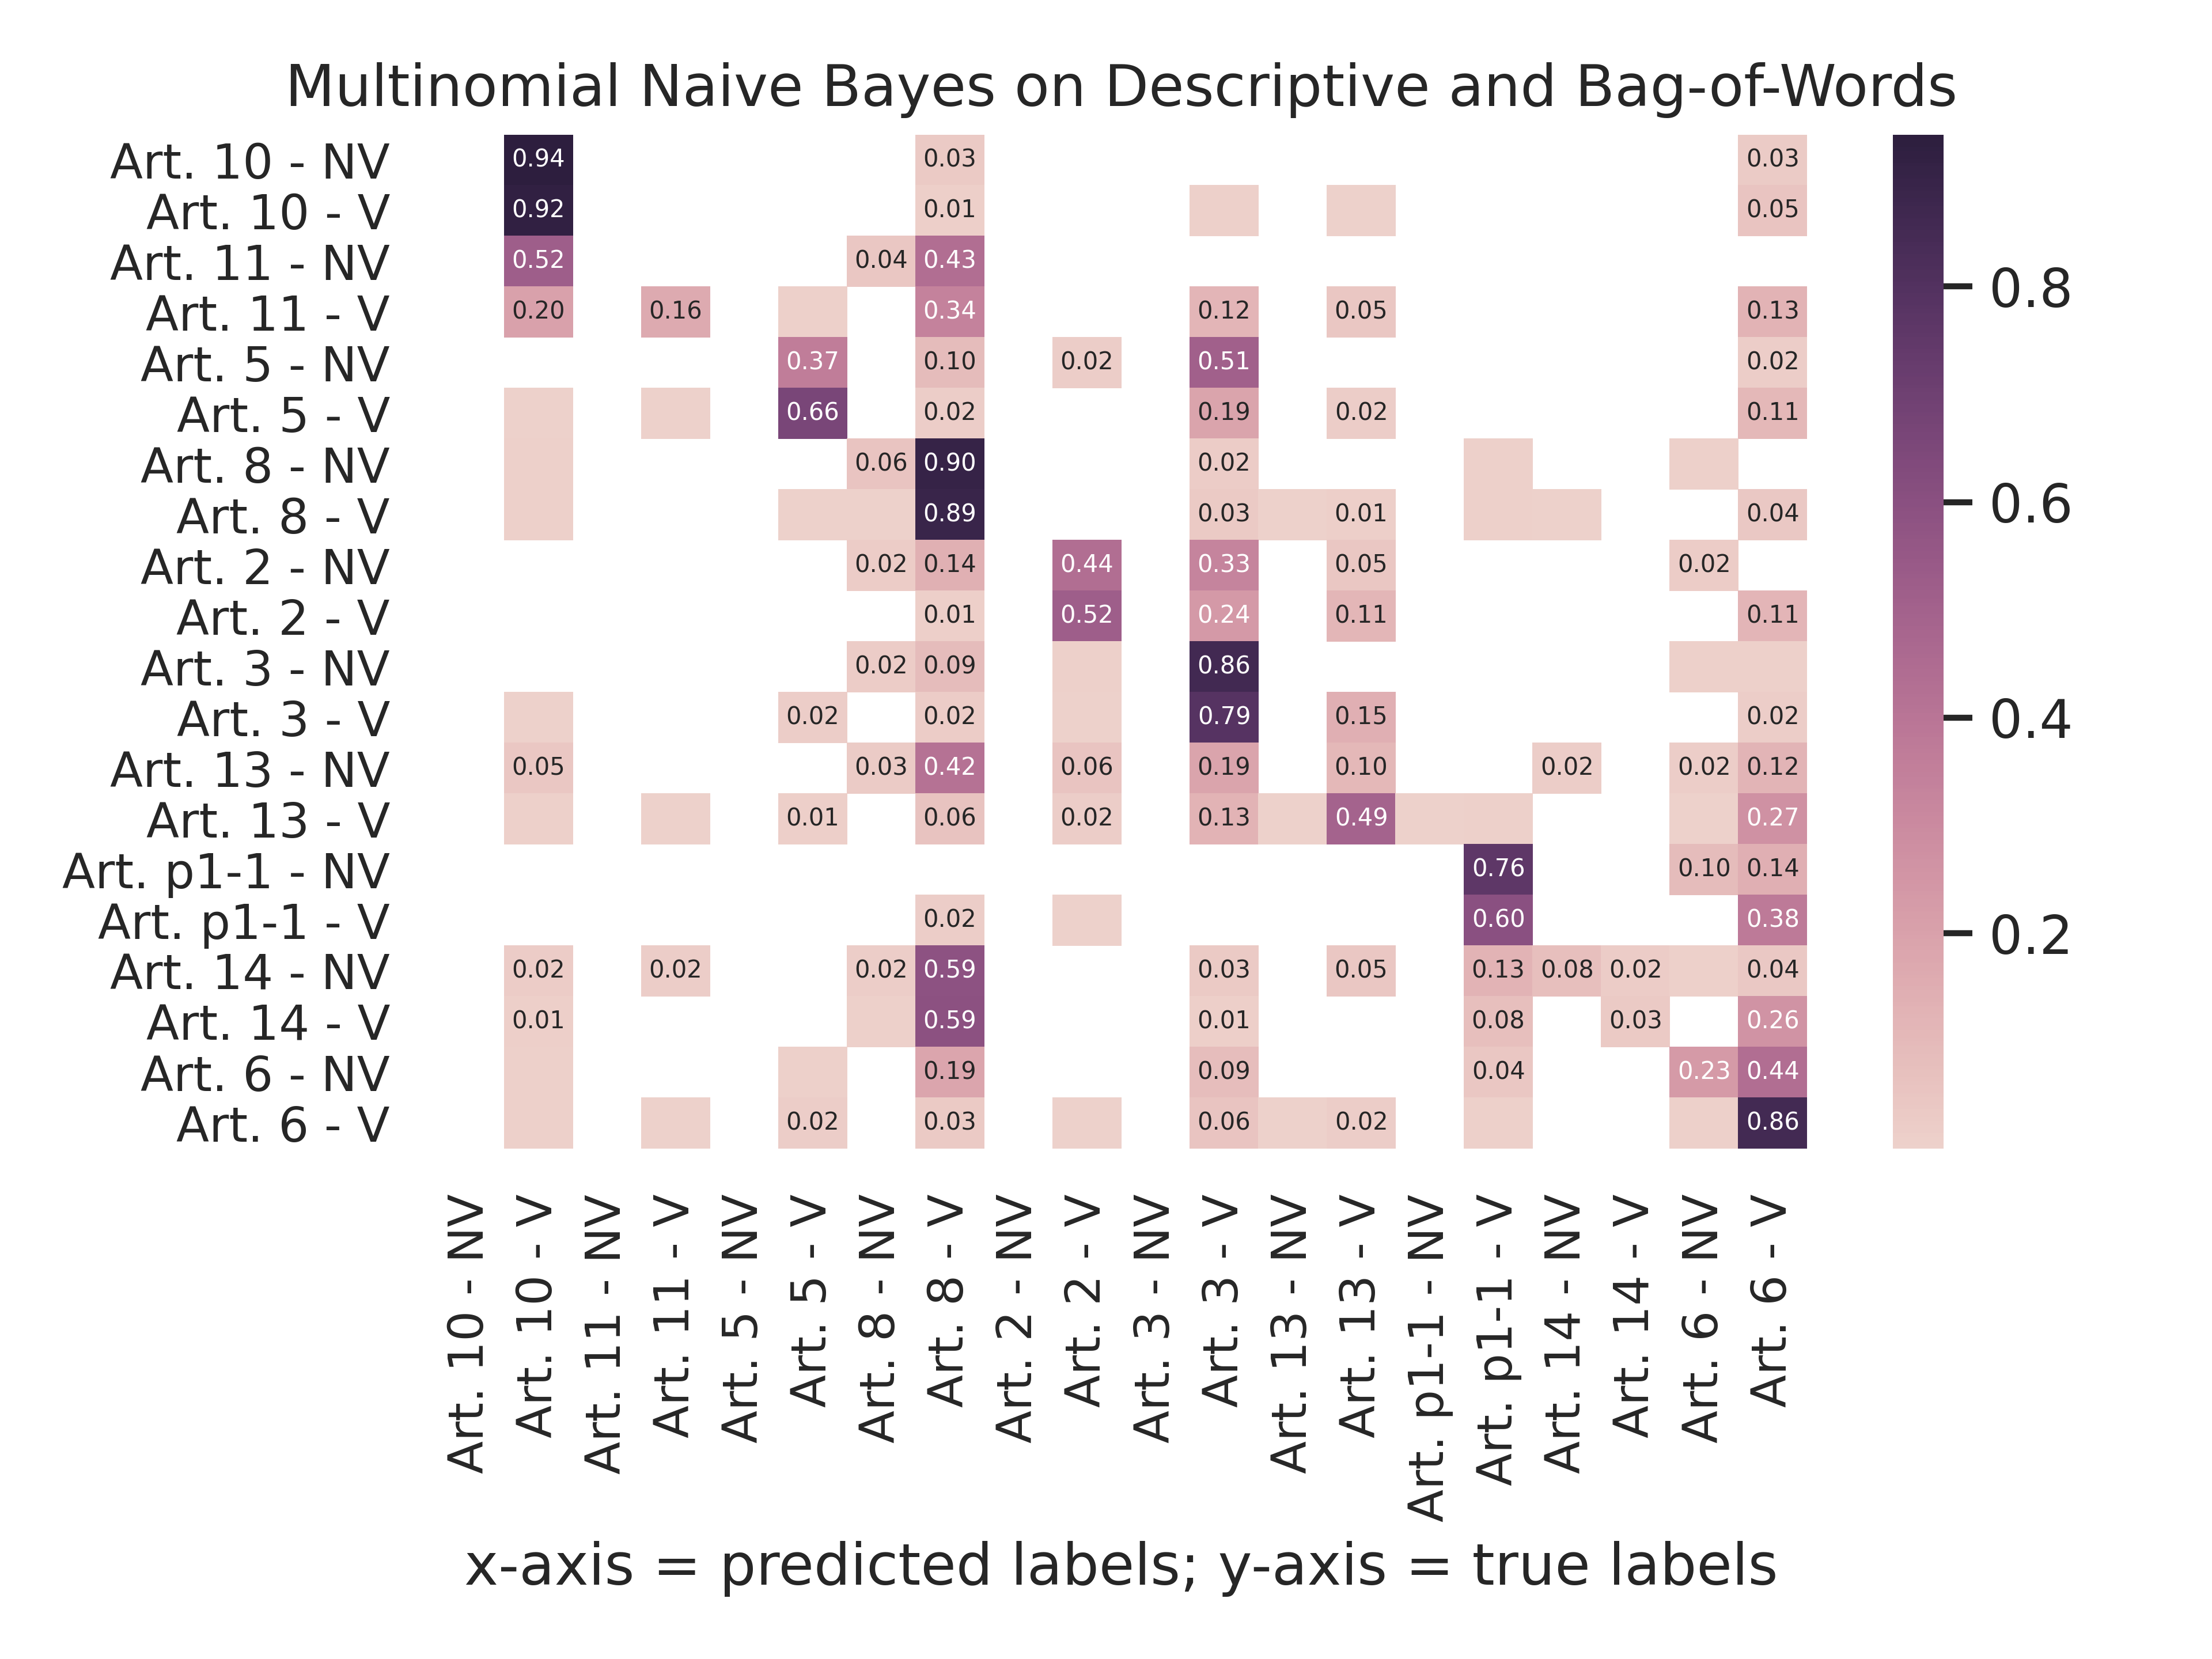
\includegraphics[scale=0.7]{data/analysis/cm/multiclass_cm_test_multinomial_naive_bayes_descriptive_and_bag-of-words.png}  
\end{figure}
\begin{figure}[!htb]
    \centering
    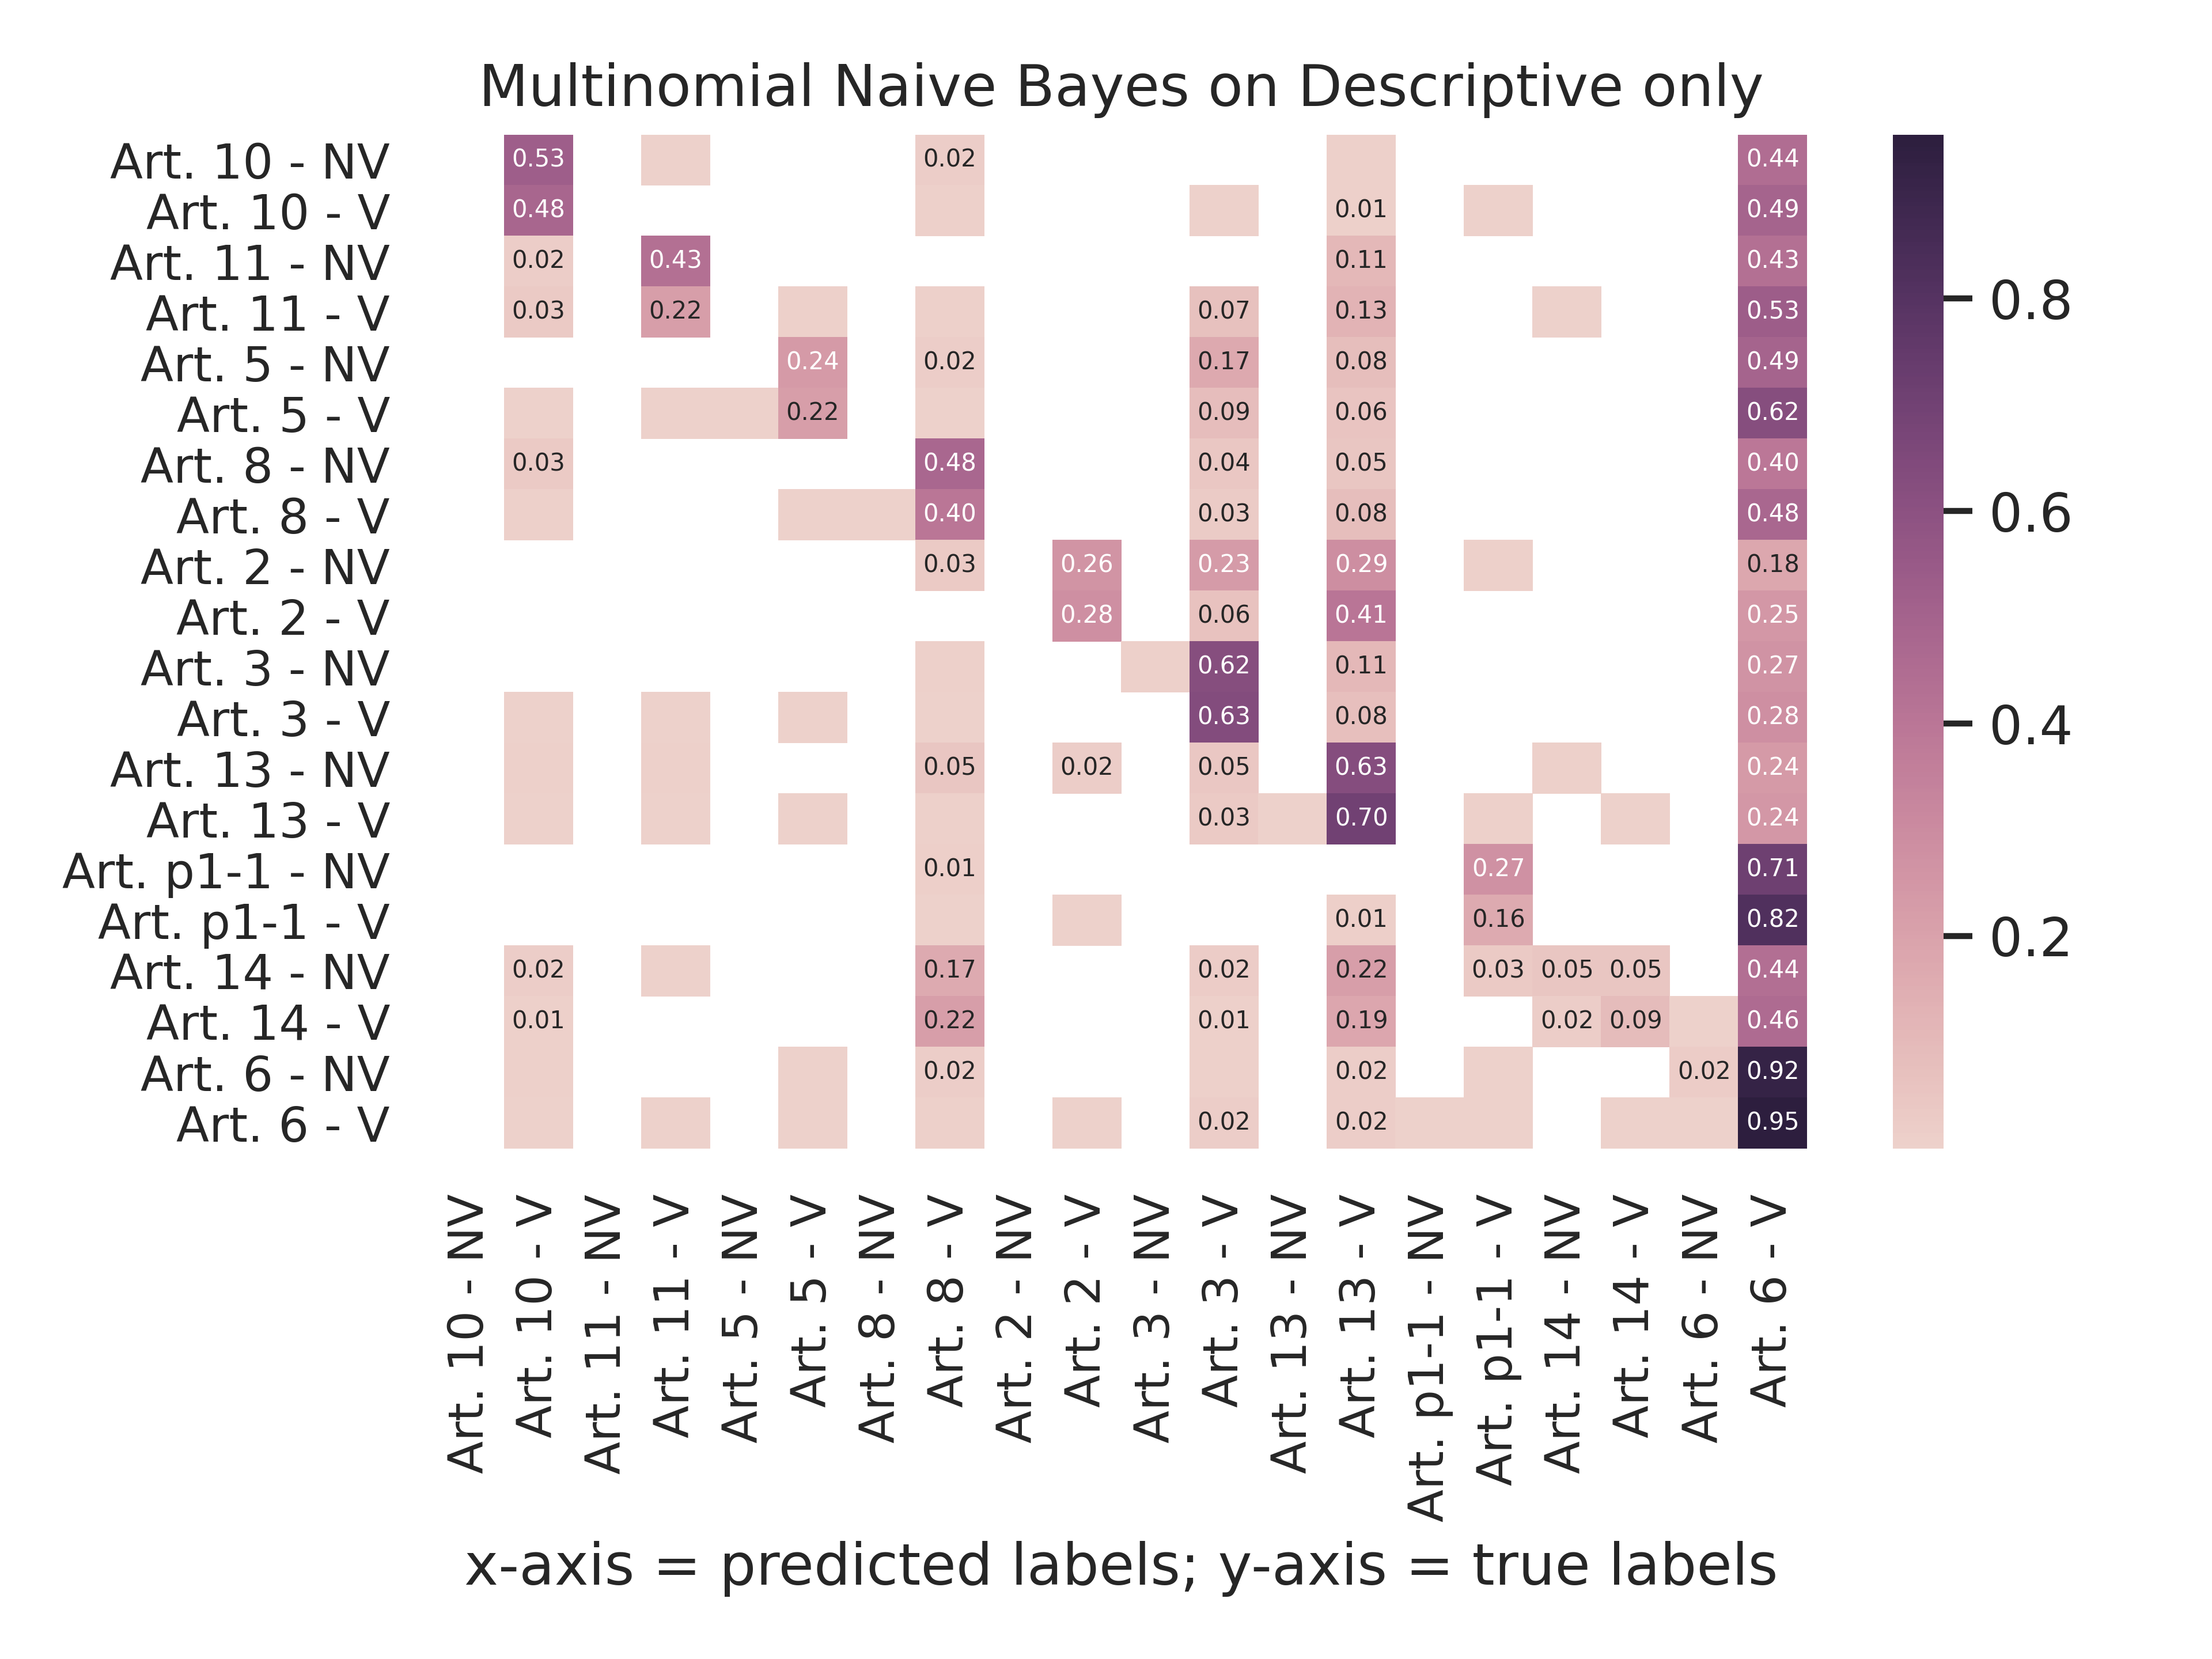
\includegraphics[scale=0.7]{data/analysis/cm/multiclass_cm_test_multinomial_naive_bayes_descriptive_only.png}  
\end{figure}
\begin{figure}[!htb]
    \centering
    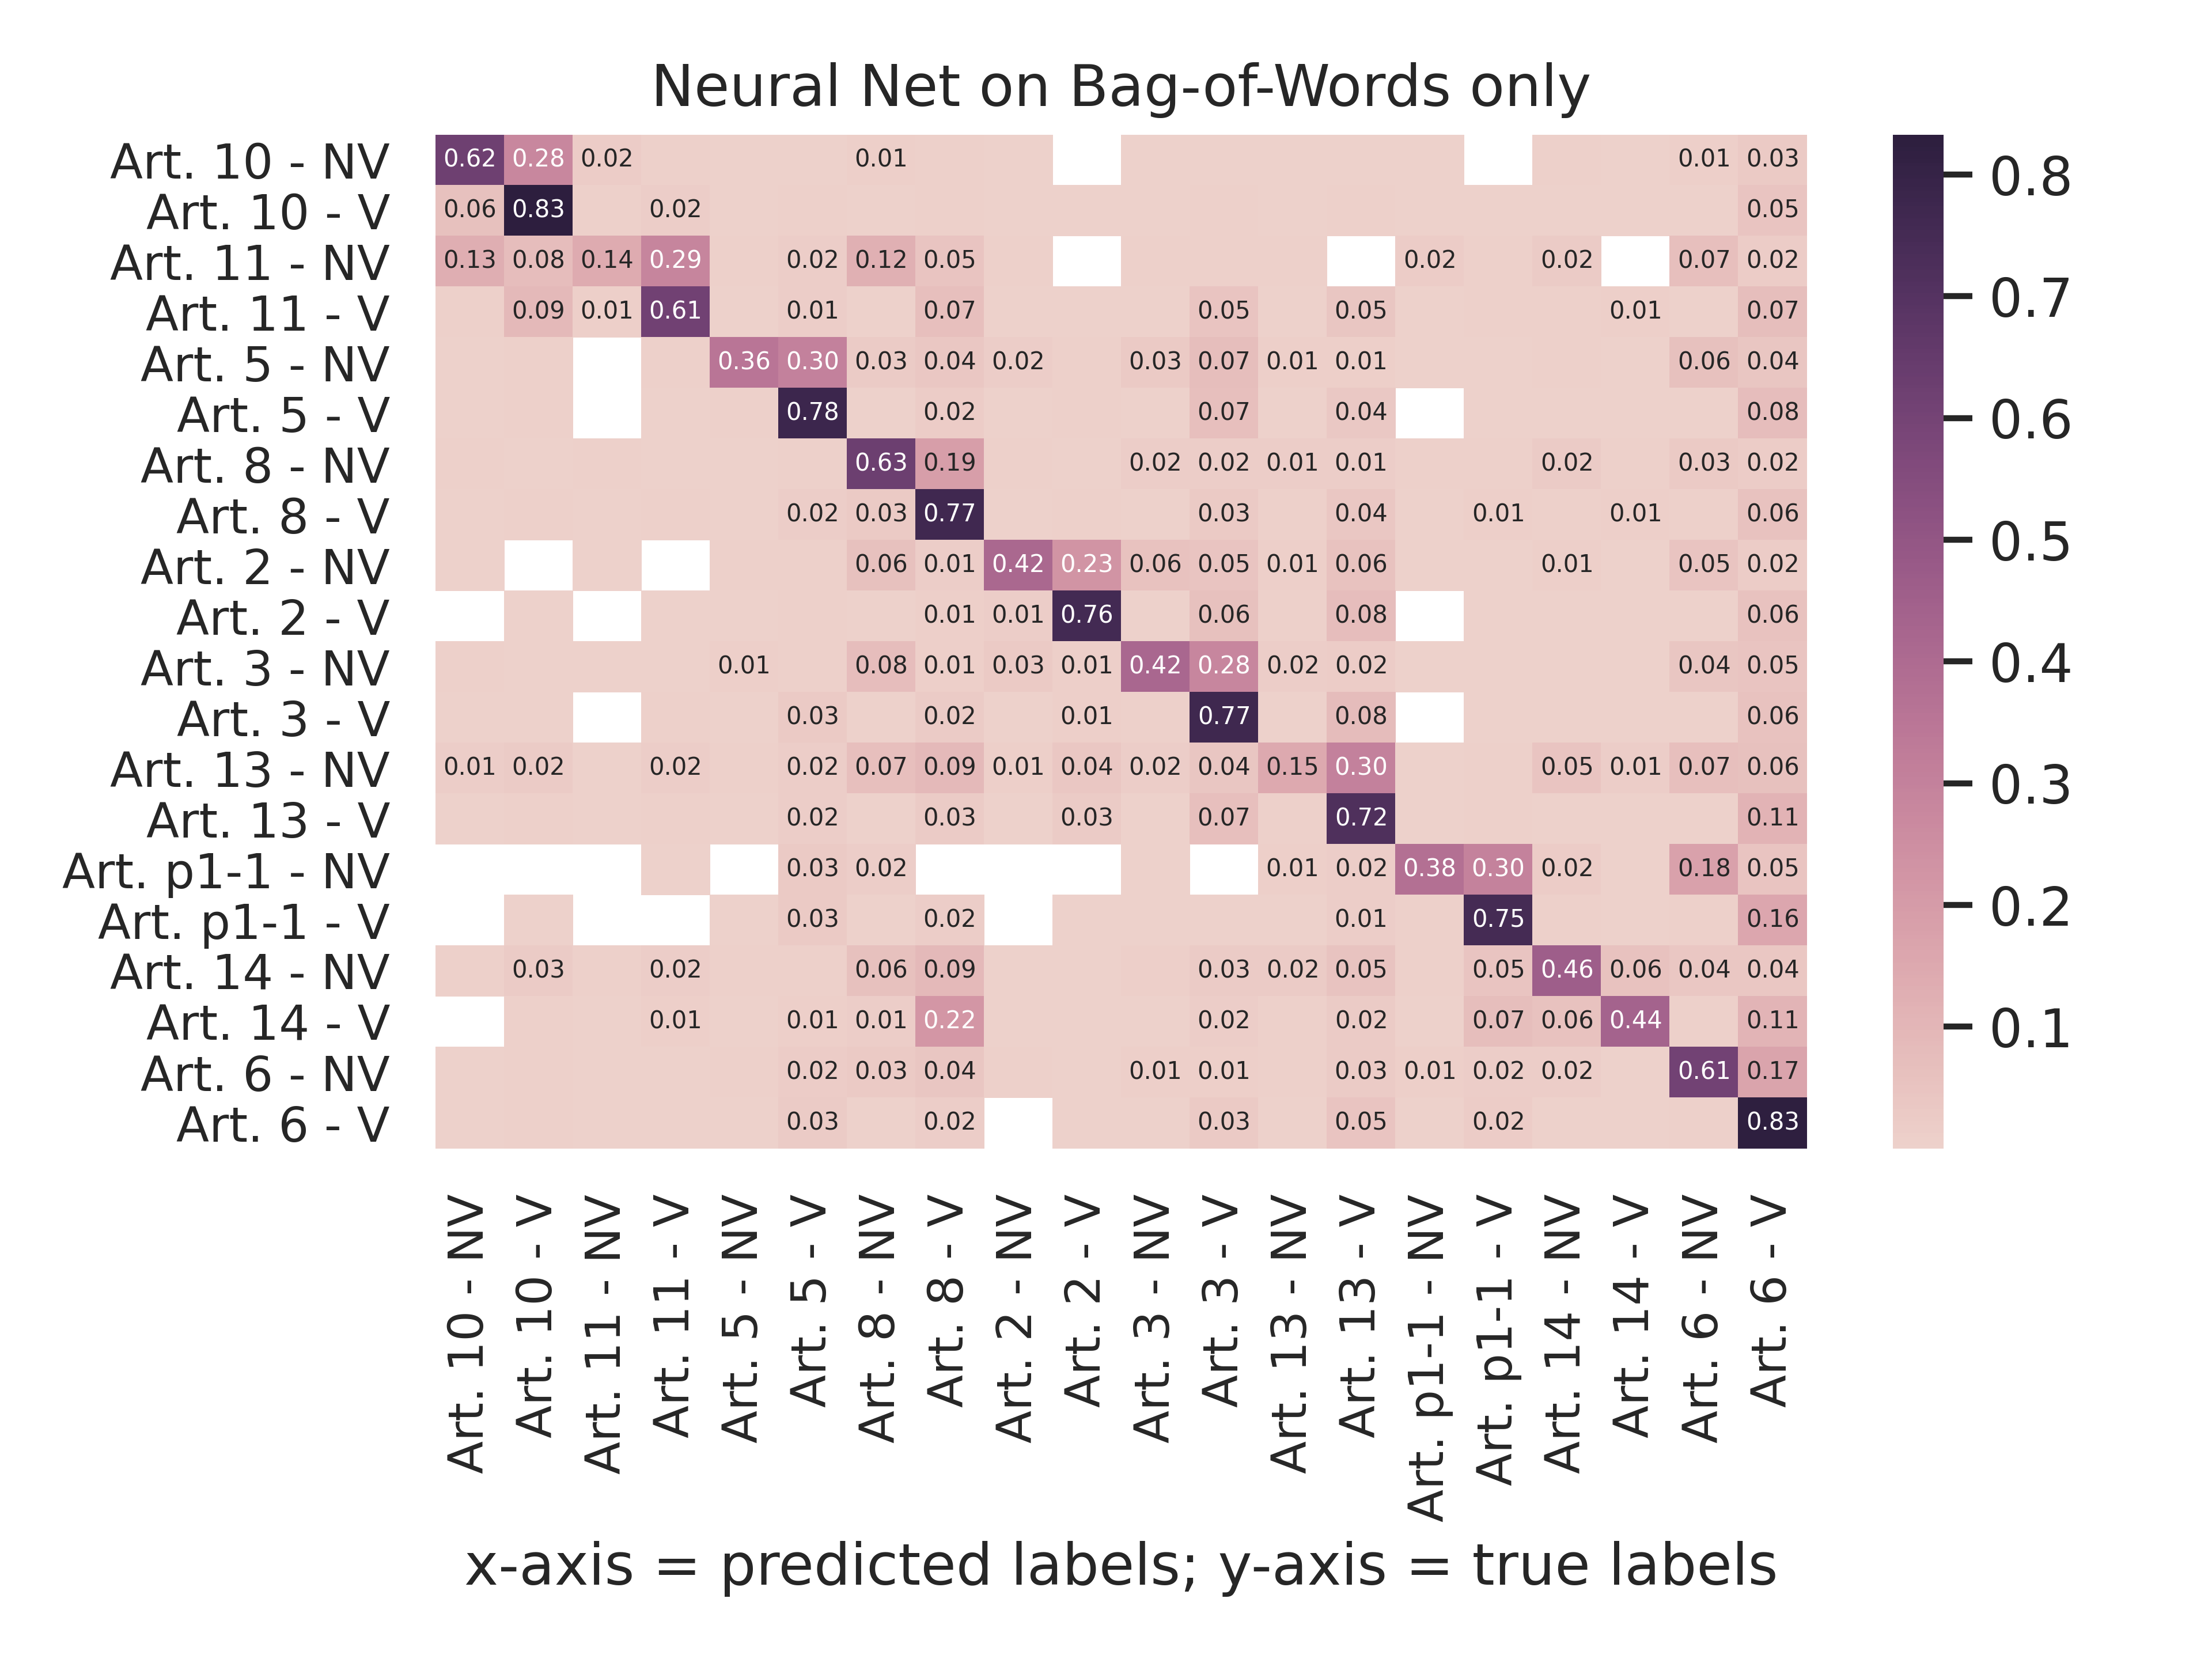
\includegraphics[scale=0.7]{data/analysis/cm/multiclass_cm_test_neural_net_bag-of-words_only.png}  
\end{figure}
\begin{figure}[!htb]
    \centering
    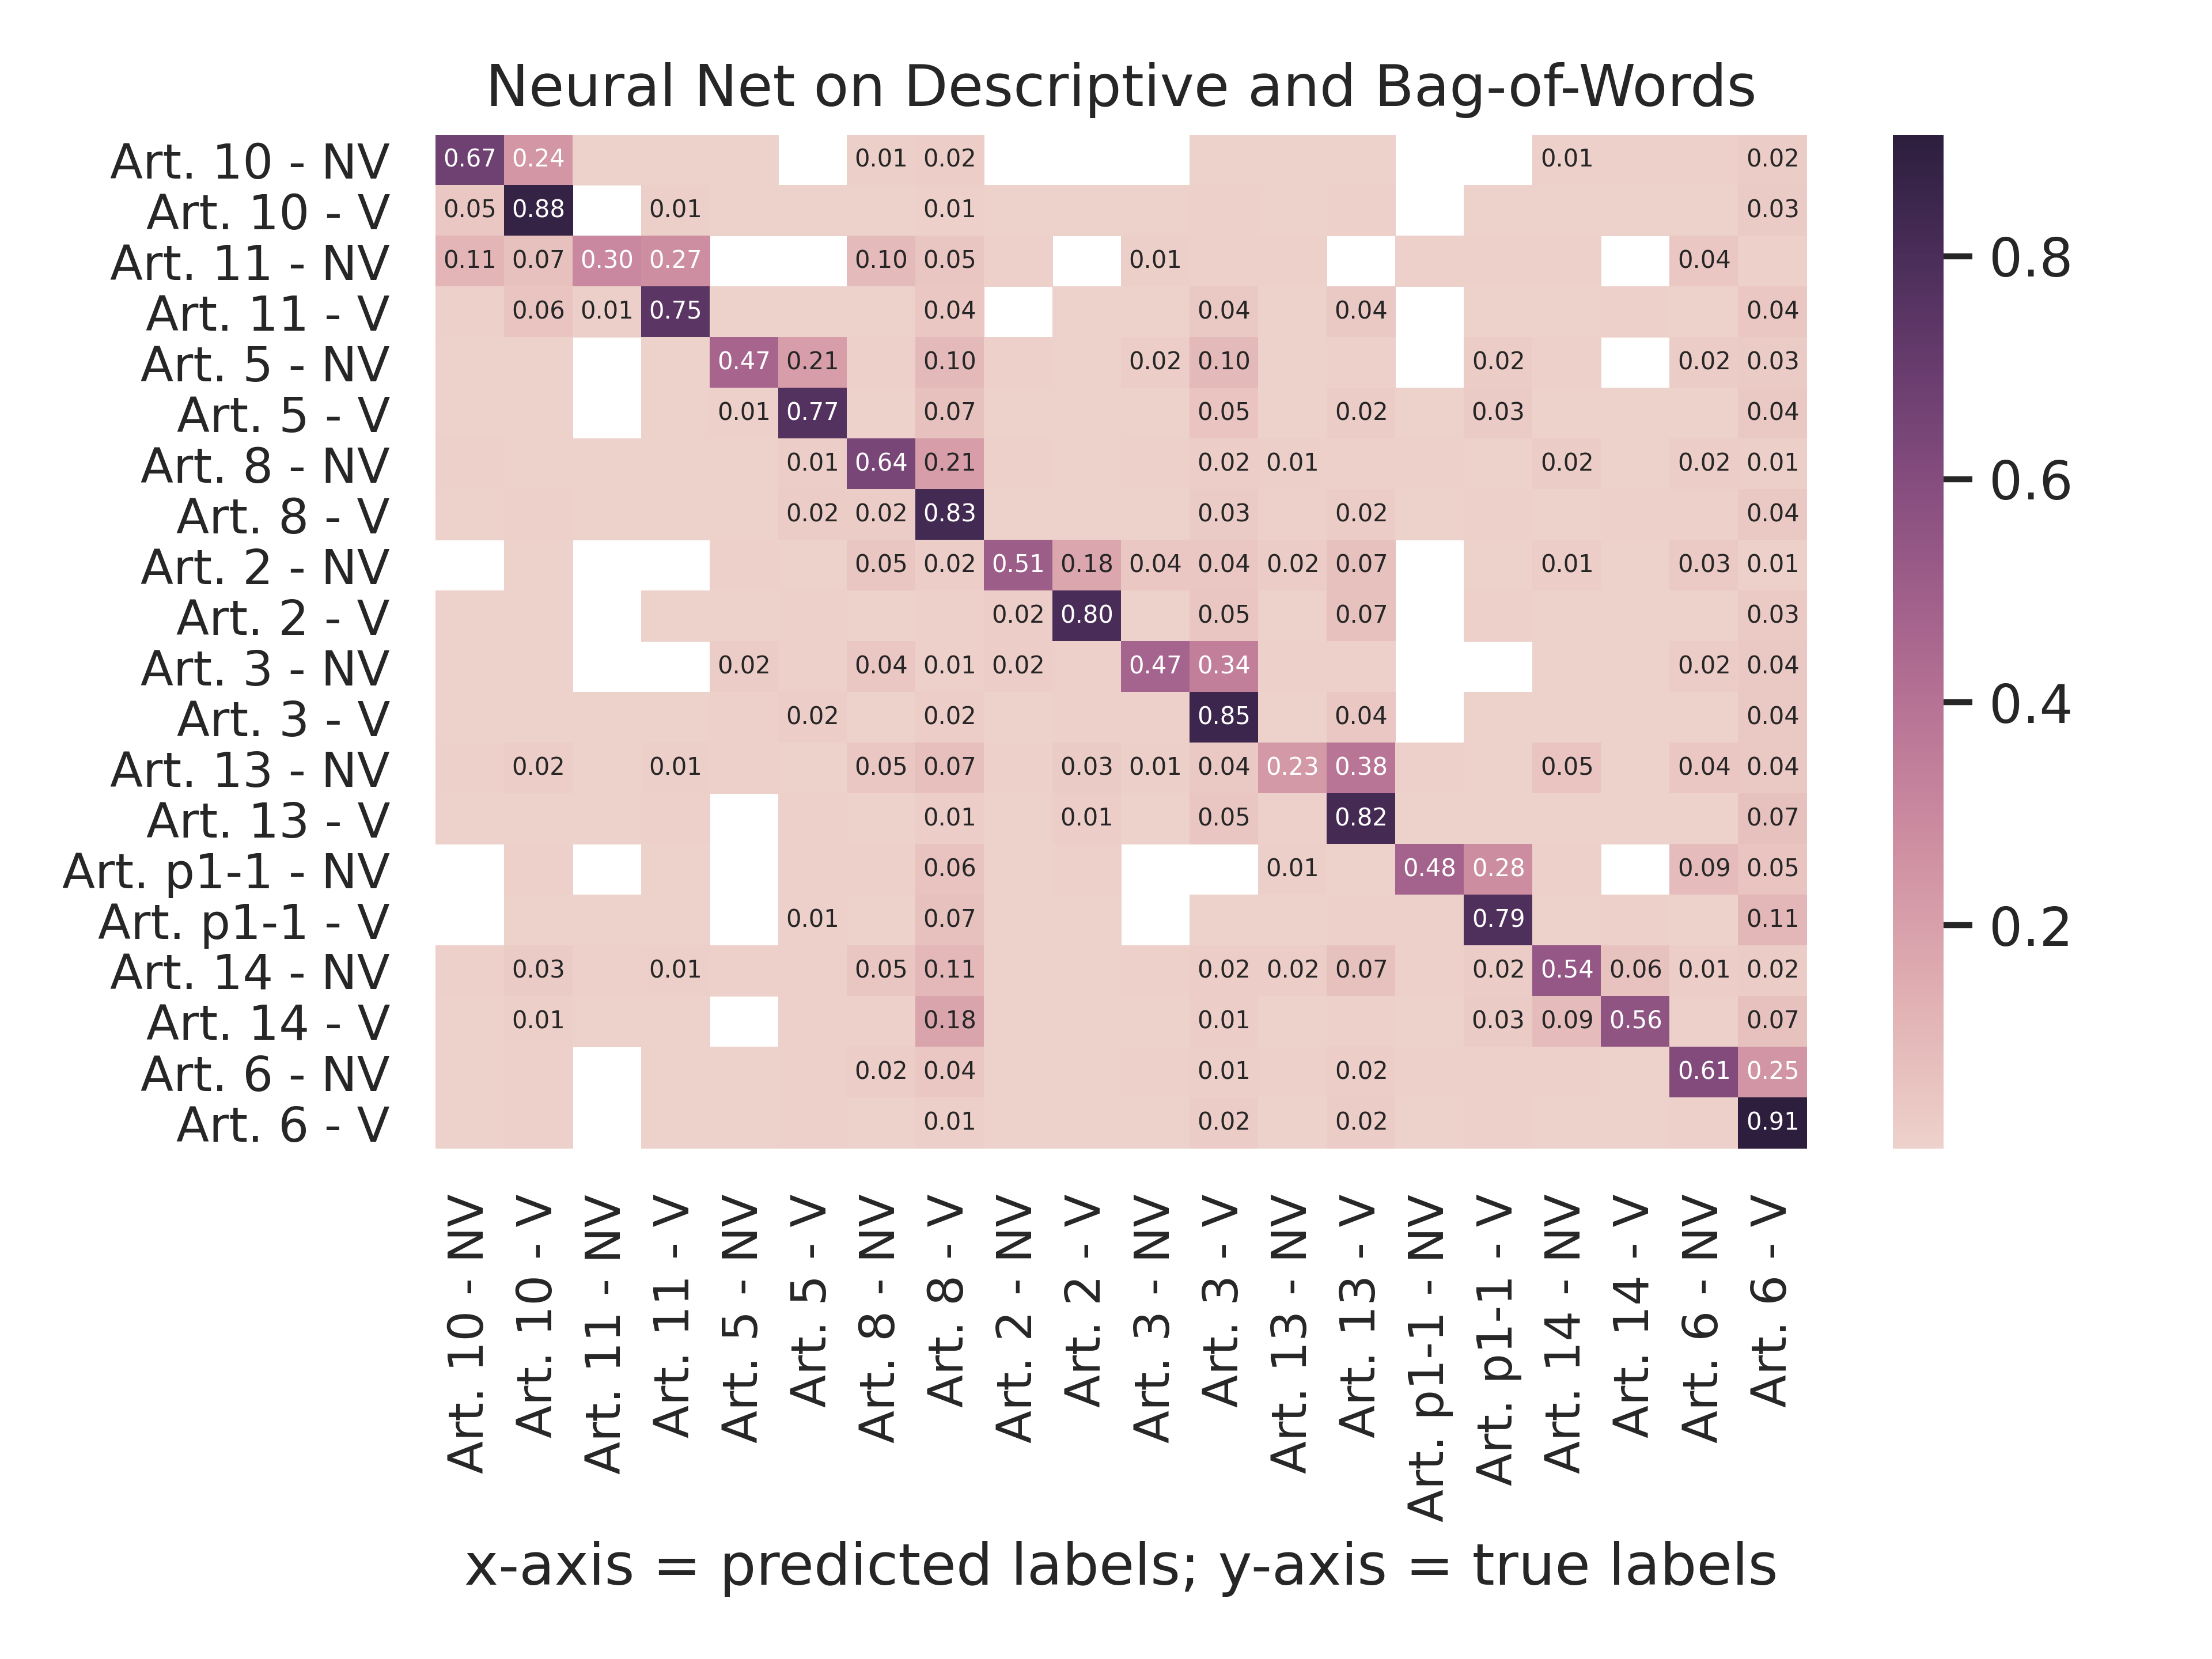
\includegraphics[scale=0.7]{data/analysis/cm/multiclass_cm_test_neural_net_descriptive_and_bag-of-words.png}  
\end{figure}
\begin{figure}[!htb]
    \centering
    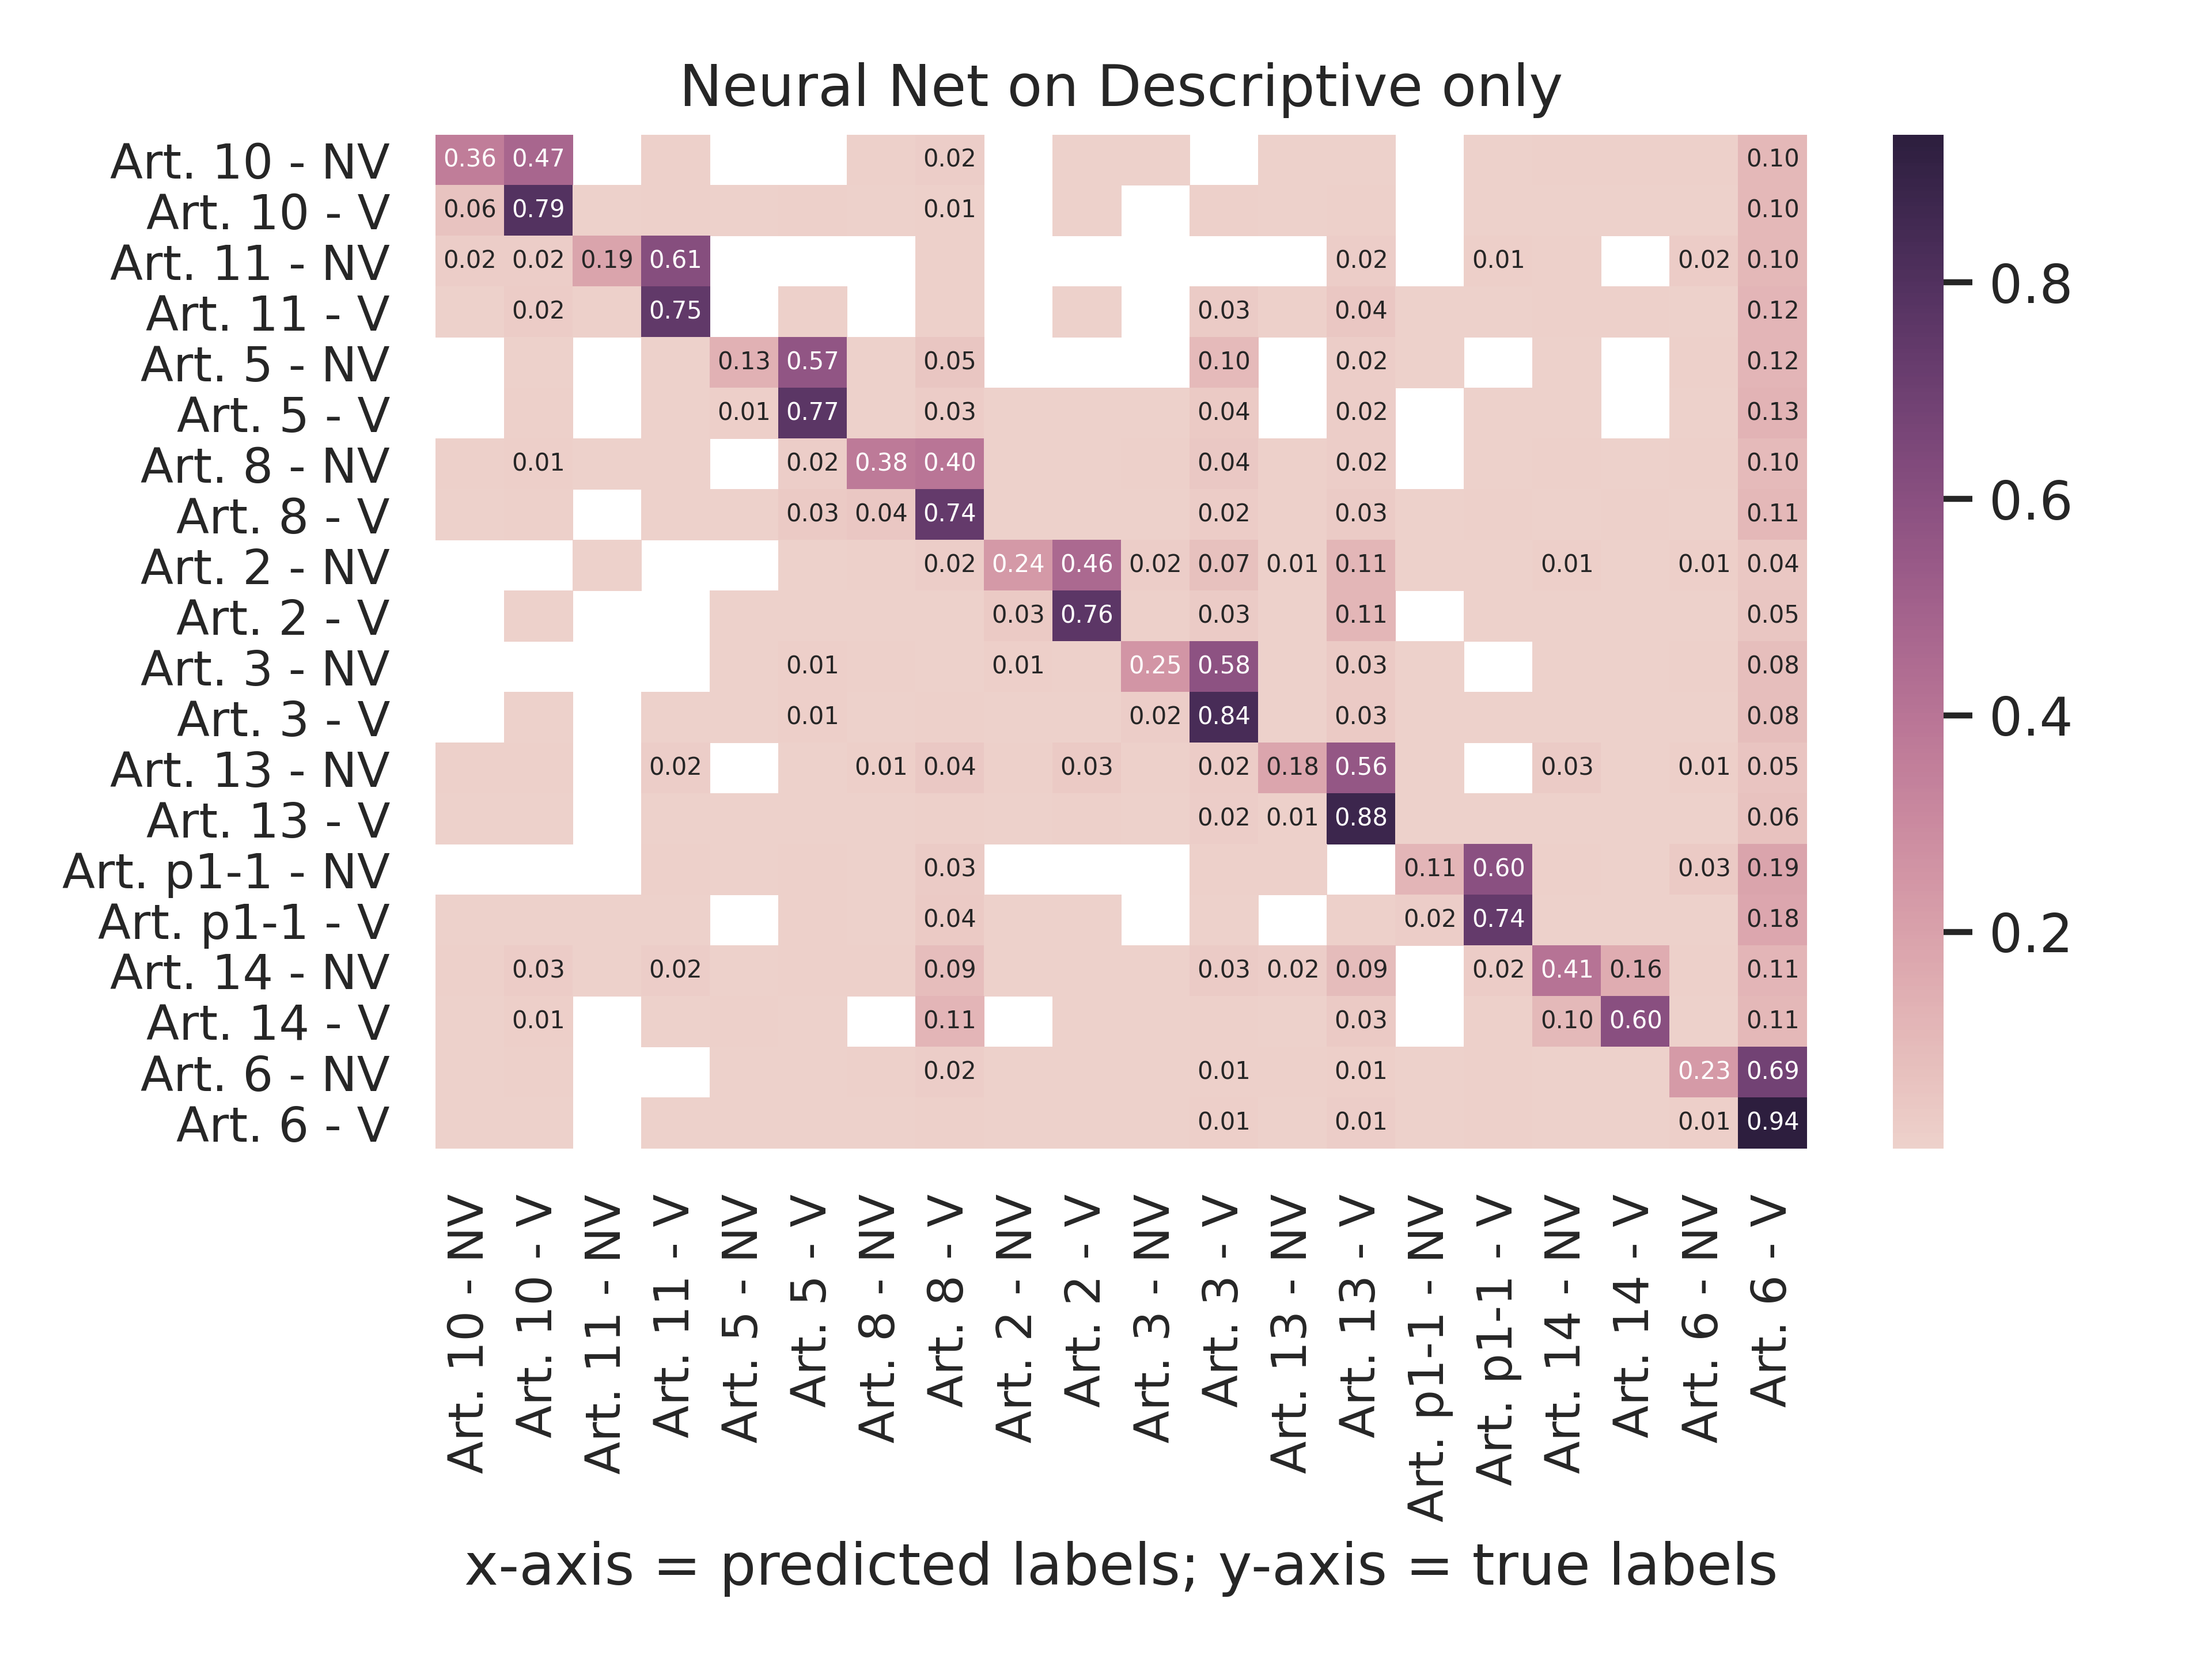
\includegraphics[scale=0.7]{data/analysis/cm/multiclass_cm_test_neural_net_descriptive_only.png}  
\end{figure}
\begin{figure}[!htb]
    \centering
    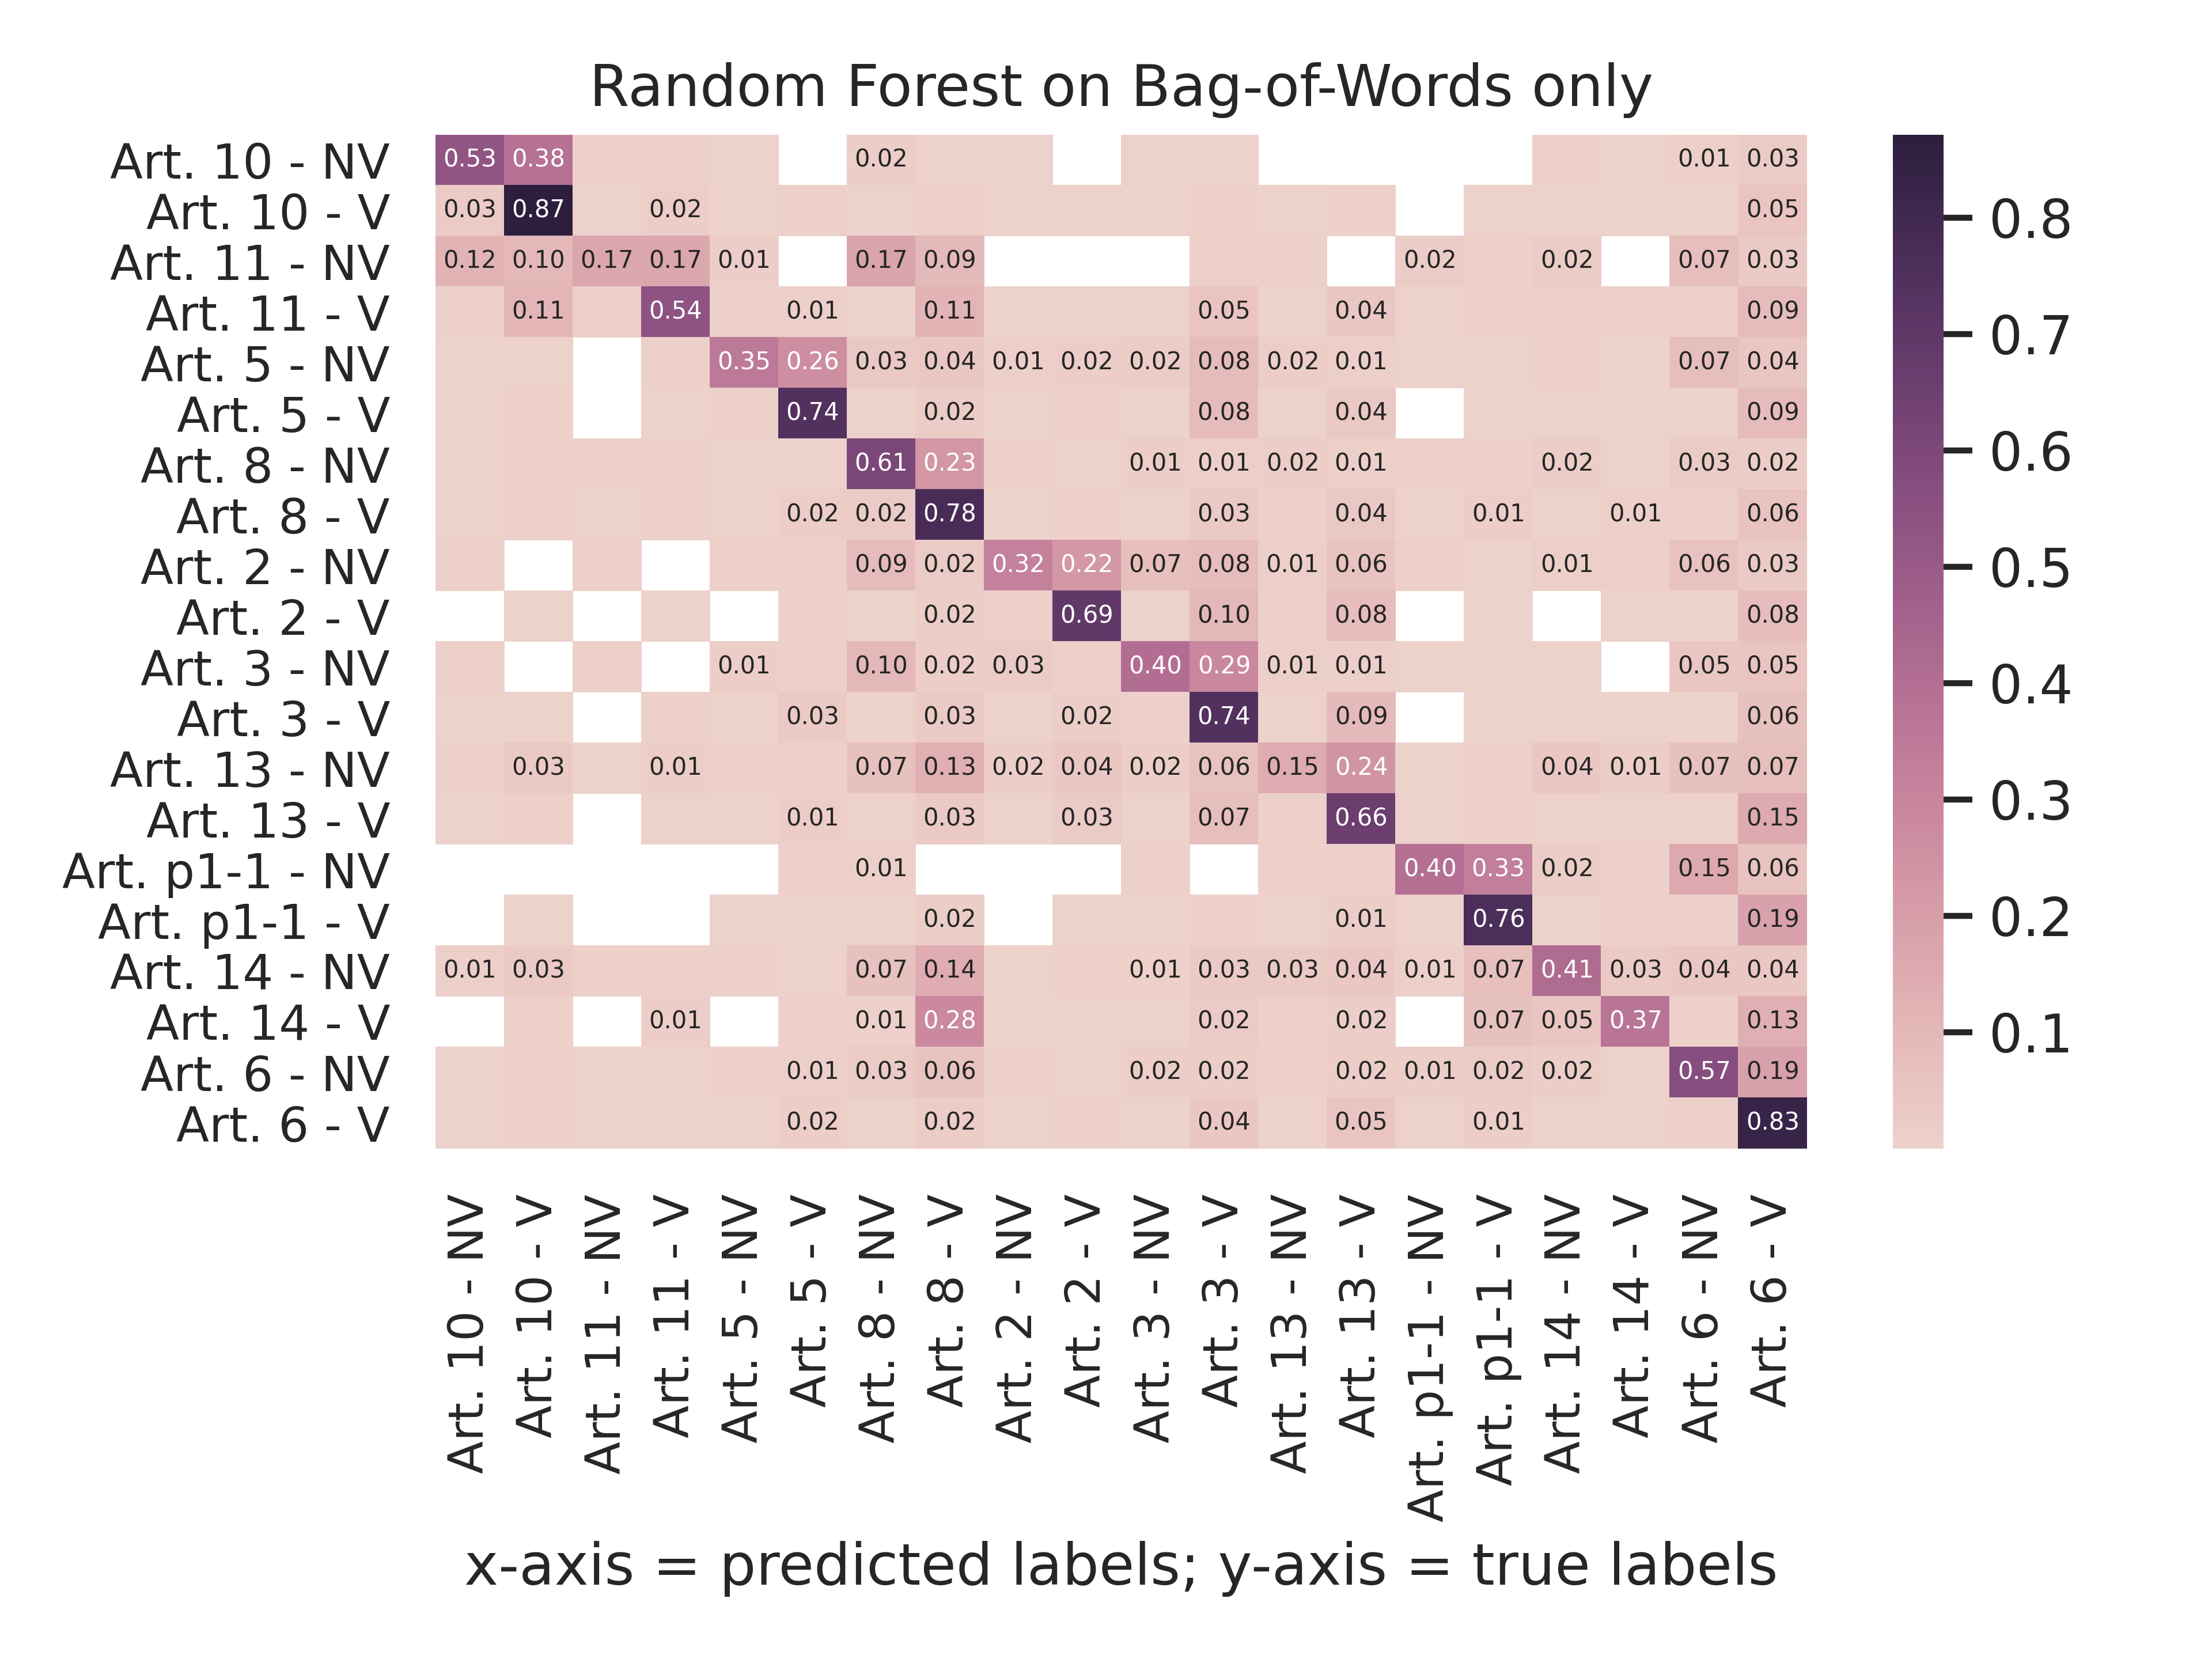
\includegraphics[scale=0.7]{data/analysis/cm/multiclass_cm_test_random_forest_bag-of-words_only.png}  
\end{figure}
\begin{figure}[!htb]
    \centering
    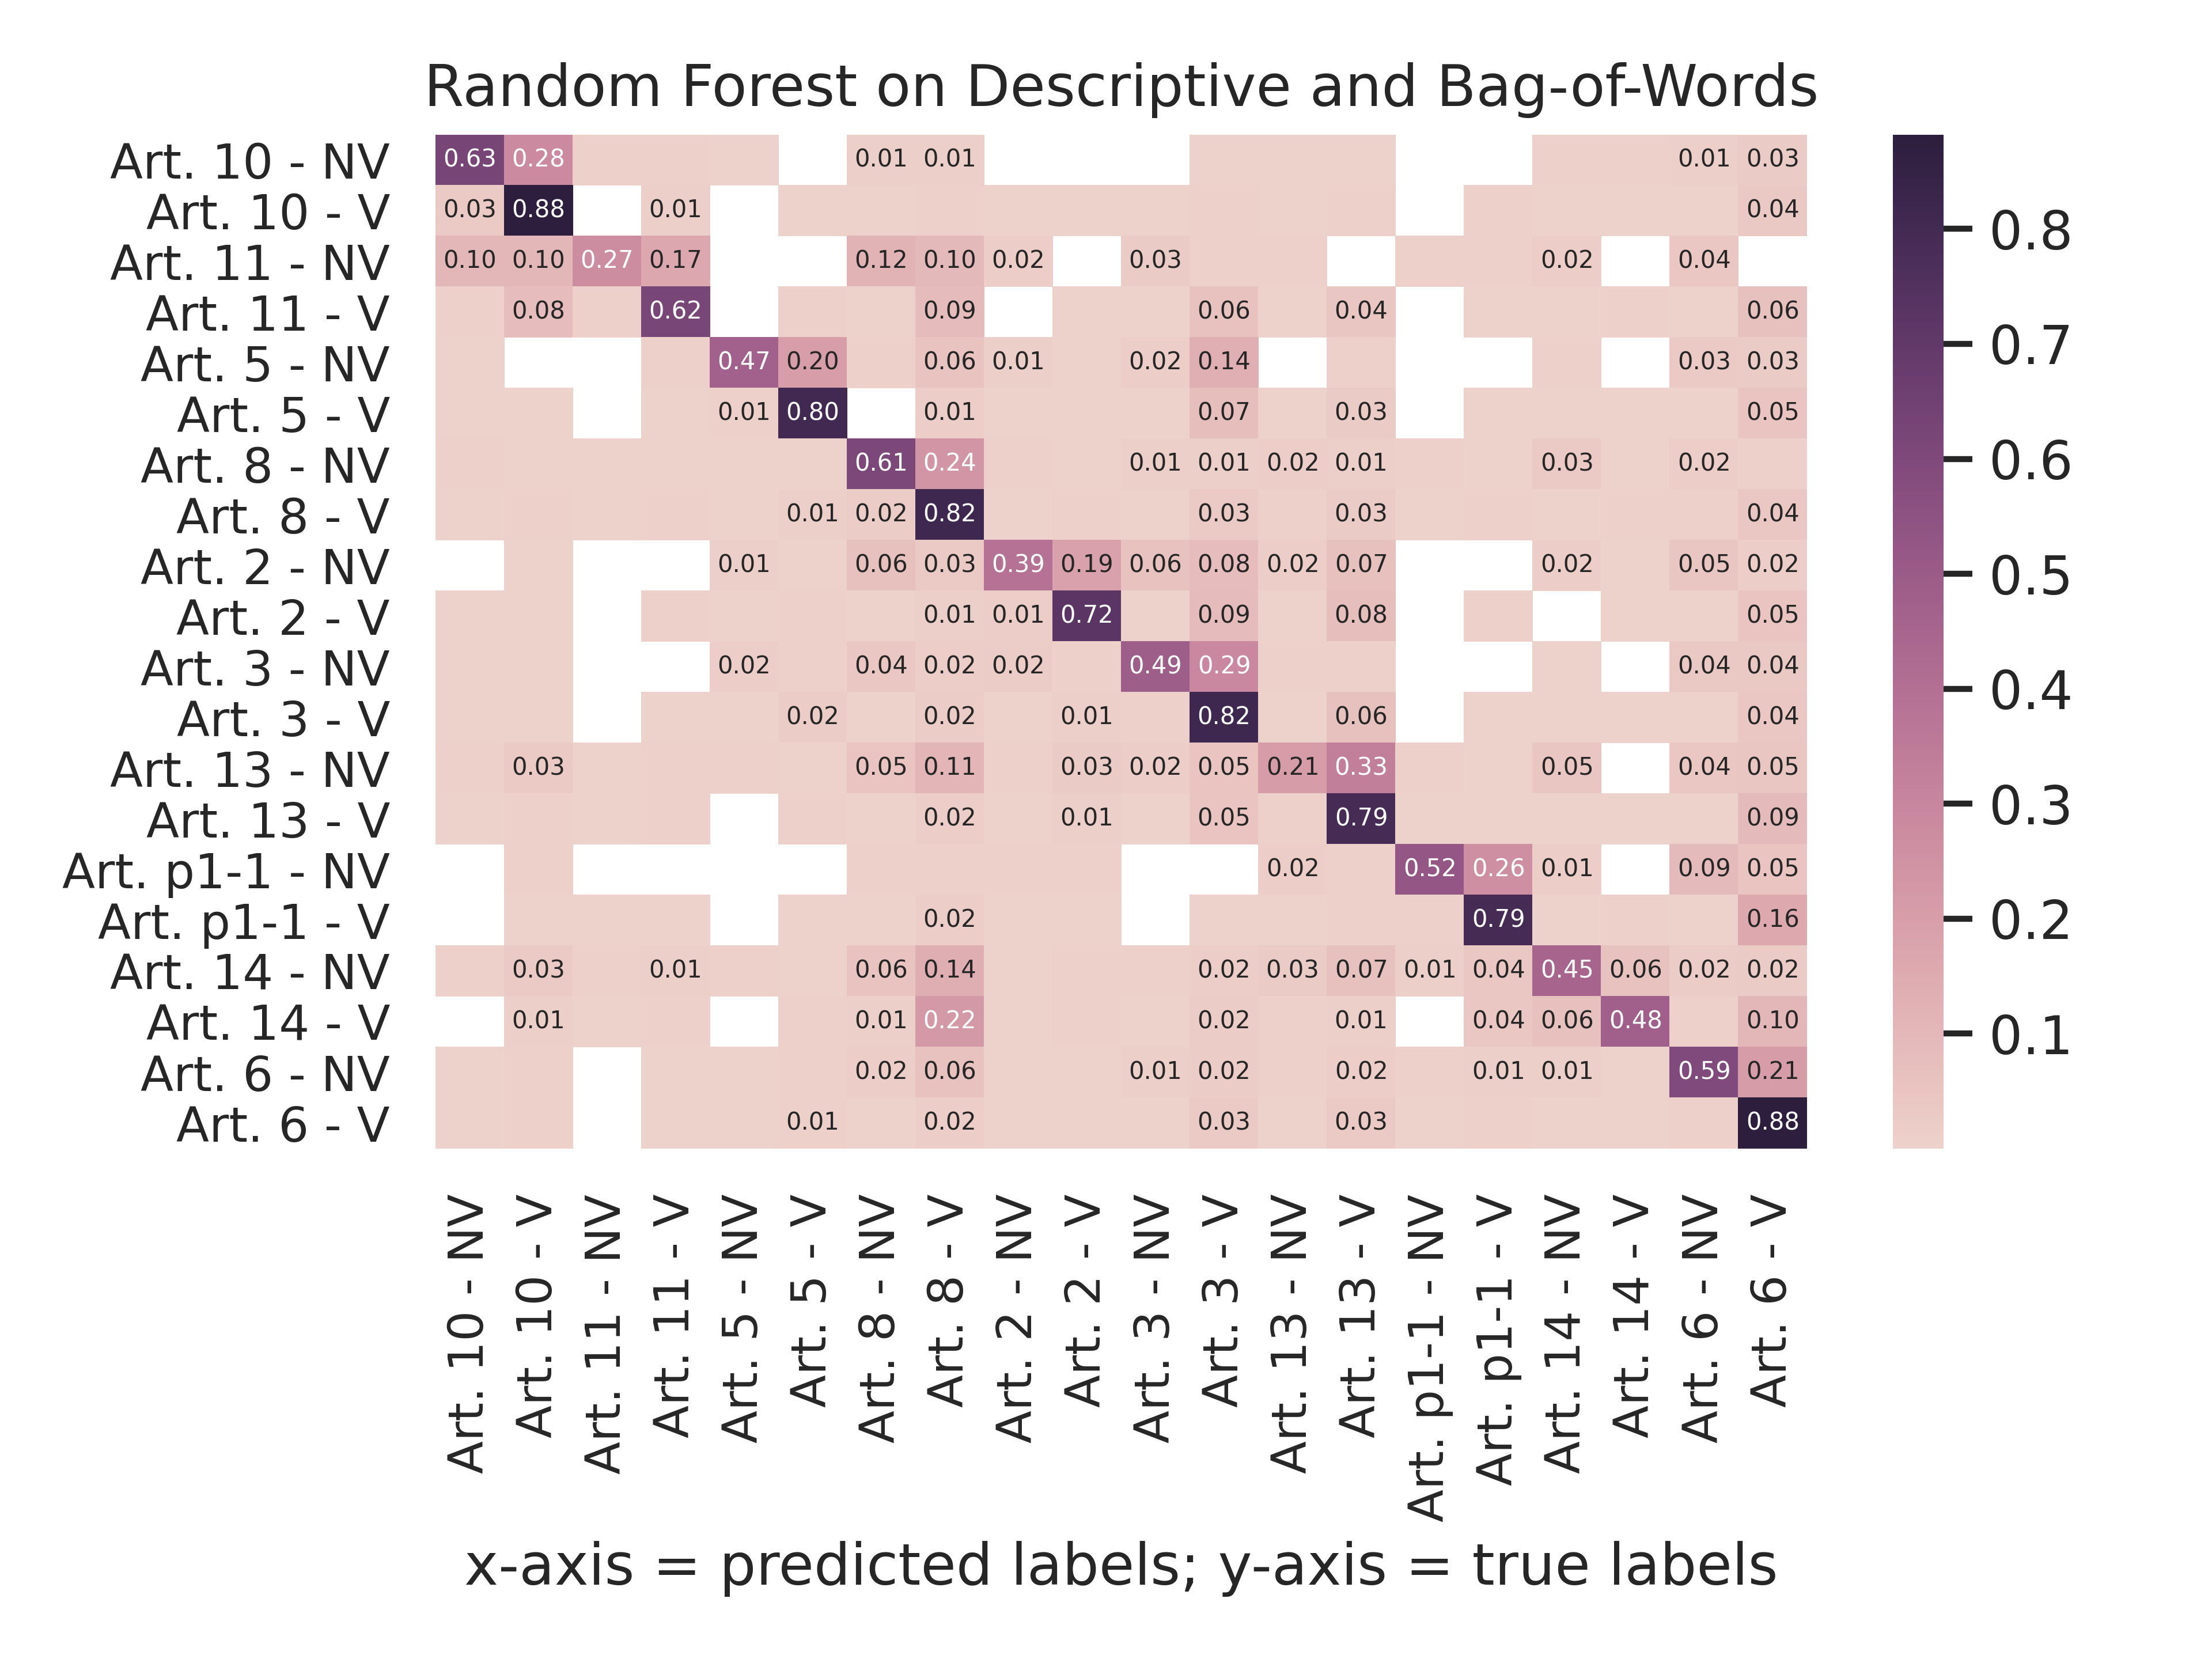
\includegraphics[scale=0.7]{data/analysis/cm/multiclass_cm_test_random_forest_descriptive_and_bag-of-words.png}  
\end{figure}
\begin{figure}[!htb]
    \centering
    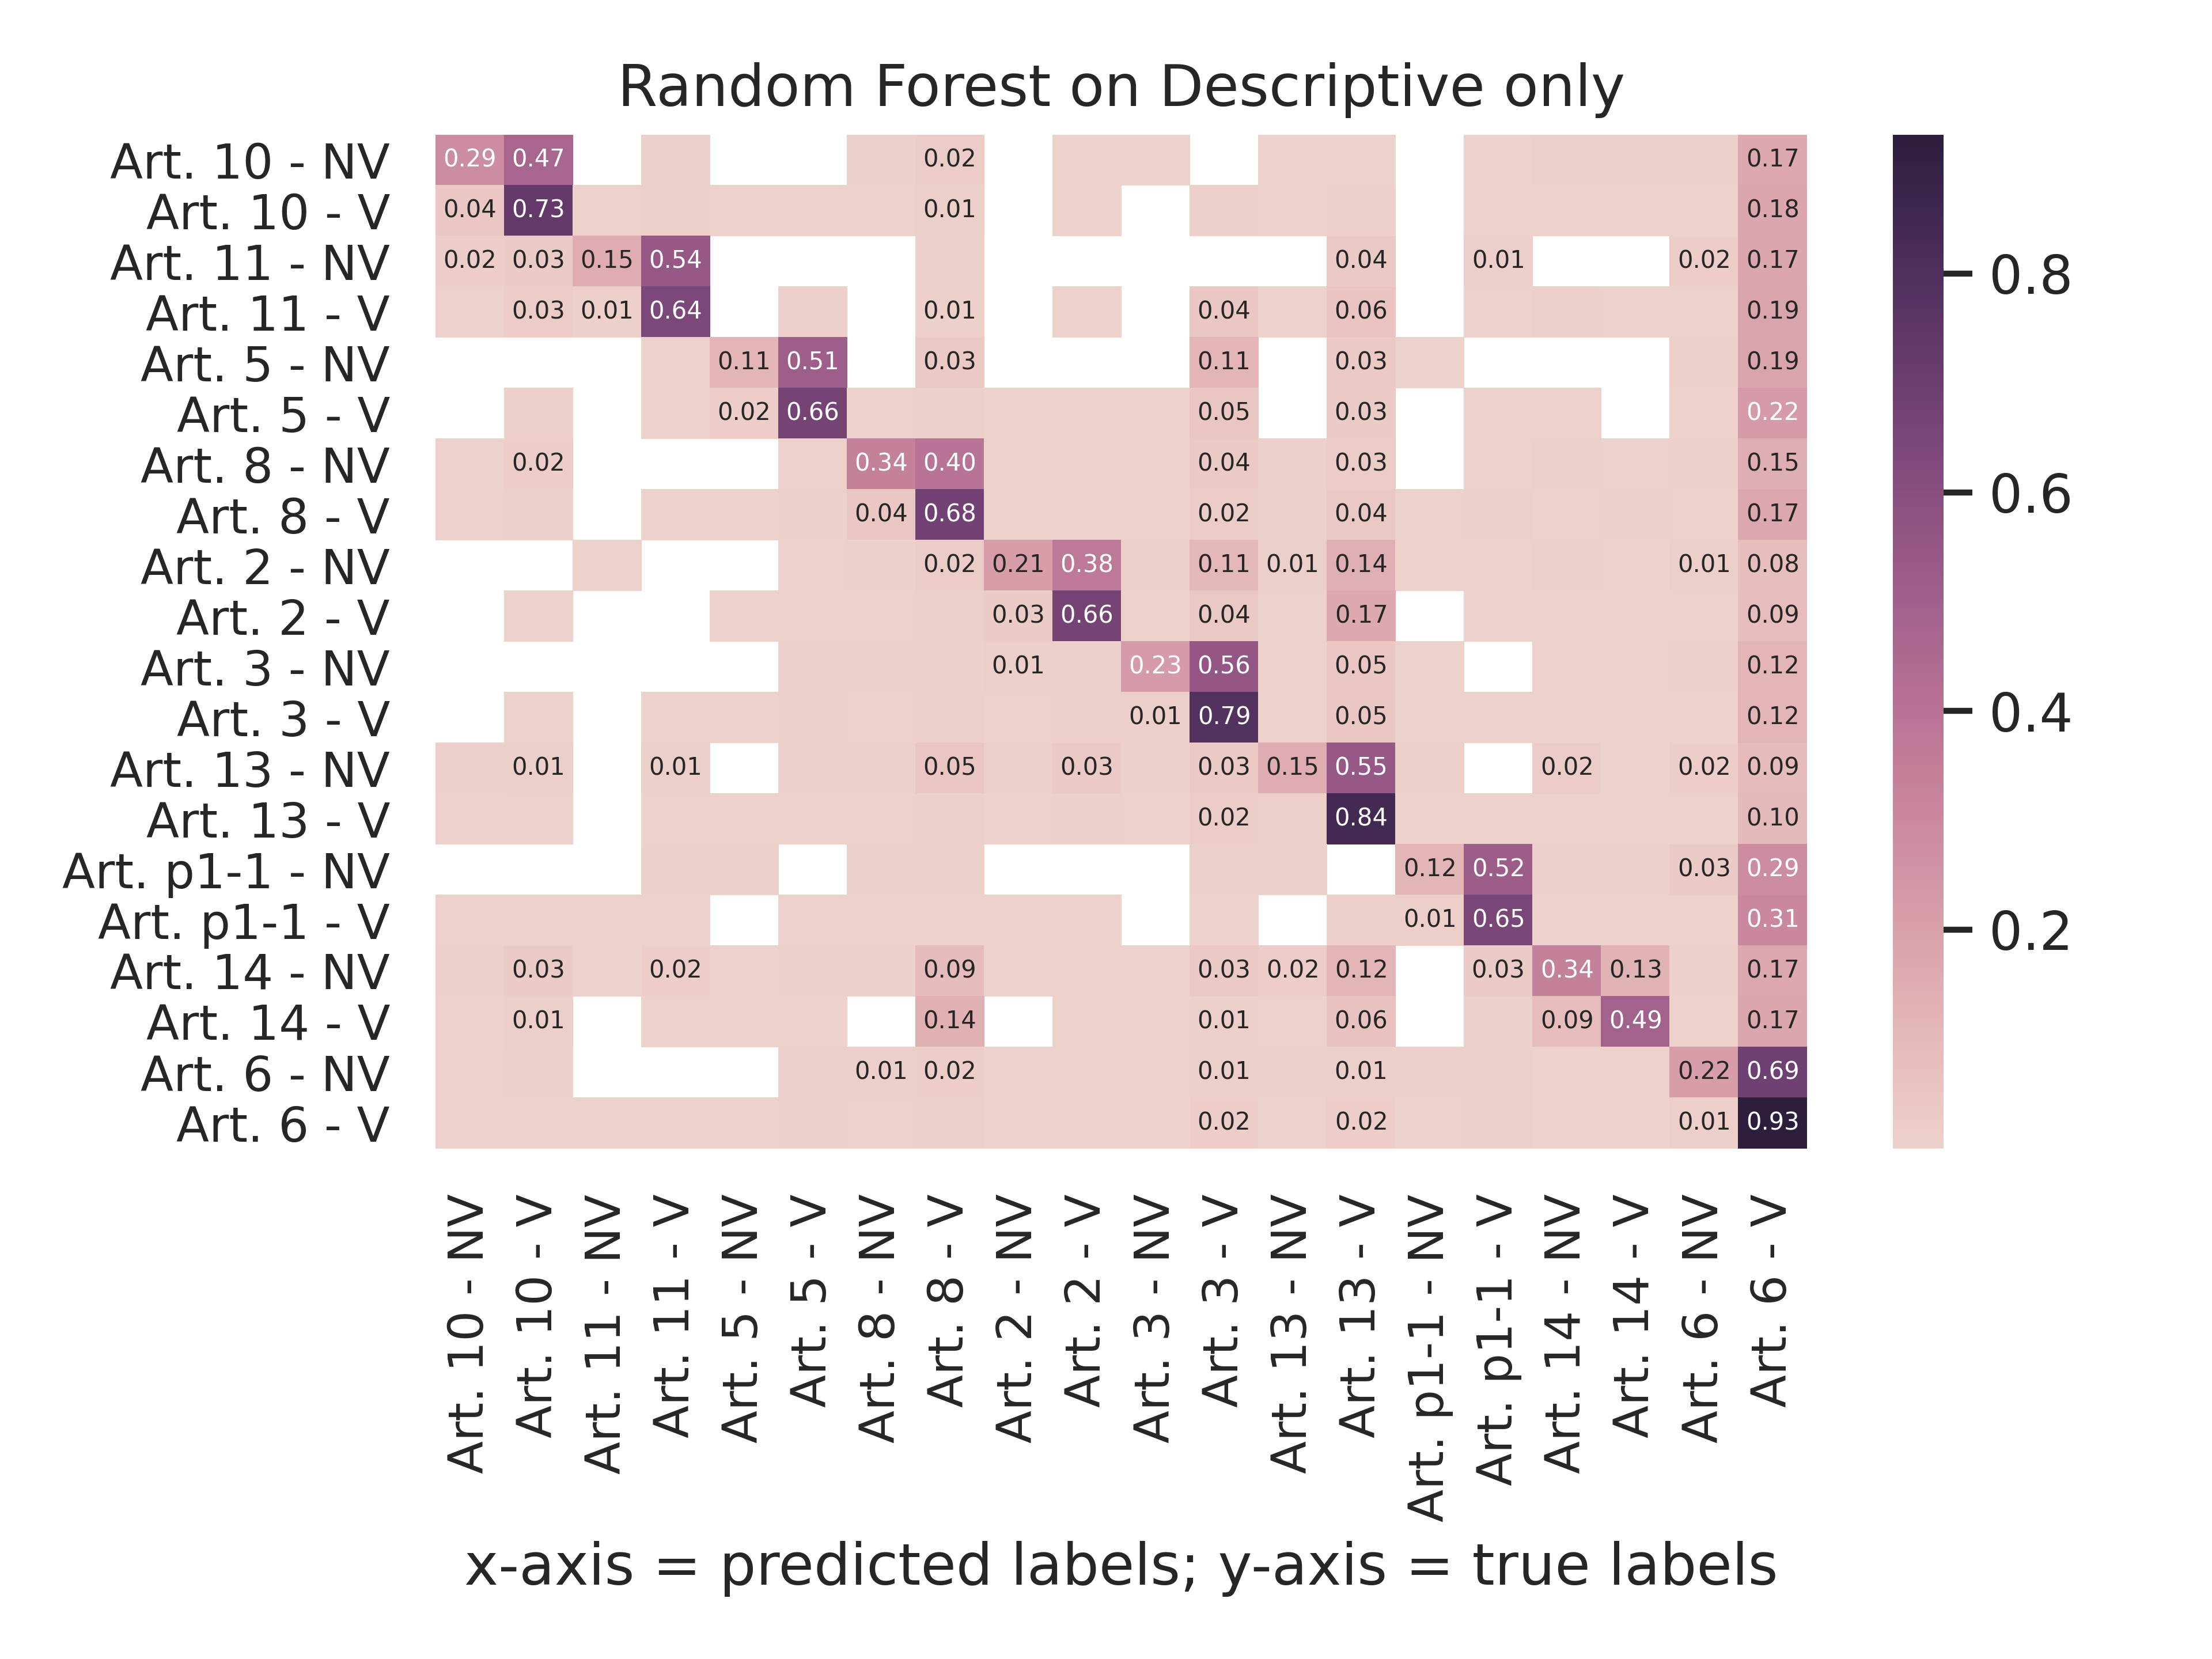
\includegraphics[scale=0.7]{data/analysis/cm/multiclass_cm_test_random_forest_descriptive_only.png}  
\end{figure}

\newpage
\section{Multilabel Classification}

This section presents the results for each method on each article and for all evaluation metrics.\\

\noindent
	\begin{tabular}{|l|l|l|l| }
\hline
 &  \multicolumn{3}{c|}{Acc - Multilabel} \\
\cline{2-4} & desc & BoW & both \\ \hline
Decision Tree       & {\bf 0.8116} (0.04) & 0.6672 (0.04) & {\bf 0.8319} (0.04)\\
Ensemble Extra Tree & 0.7425 (0.06) & 0.6546 (0.04) & 0.6856 (0.05)\\
Extra Tree          & 0.6045 (0.05) & 0.5318 (0.05) & 0.5402 (0.04)\\
Neural Net          & 0.7511 (0.05) & {\bf 0.6845} (0.04) & 0.7339 (0.05)\\
Random Forest       & 0.7281 (0.06) & 0.6342 (0.04) & 0.6655 (0.04)\\
\hline
\end{tabular}~\\
	\begin{tabular}{|l|l|l|l| }
\hline
 &  \multicolumn{3}{c|}{F1 Weighted - Multilabel} \\
\cline{2-4} & desc & BoW & both \\ \hline
Decision Tree       & {\bf 0.8678} & 0.7807 & {\bf 0.8903}\\
Ensemble Extra Tree & 0.8372 & 0.7917 & 0.8124\\
Extra Tree          & 0.7221 & 0.6634 & 0.6701\\
Neural Net          & 0.8568 & {\bf 0.8301} & 0.8556\\
Random Forest       & 0.8271 & 0.7766 & 0.7985\\
\hline
\end{tabular}~\\
	\begin{tabular}{|l|l|l|l| }
\hline
 &  \multicolumn{3}{c|}{Hamming Loss - Multilabel} \\
\cline{2-4} & desc & BoW & both \\ \hline
Decision Tree       & {\bf 0.0068} & 0.0112 & {\bf 0.0056}\\
Ensemble Extra Tree & 0.0075 & 0.0093 & 0.0084\\
Extra Tree          & 0.0139 & 0.0170 & 0.0167\\
Neural Net          & 0.0069 & {\bf 0.0081} & 0.0068\\
Random Forest       & 0.0080 & 0.0099 & 0.0089\\
\hline
\end{tabular}~\\
	\begin{tabular}{|l|l|l|l| }
\hline
 &  \multicolumn{3}{c|}{Jaccard Similarity Score - Multilabel} \\
\cline{2-4} & desc & BoW & both \\ \hline
Decision Tree       & {\bf 0.7674} & 0.6412 & {\bf 0.8033}\\
Ensemble Extra Tree & 0.7225 & 0.6566 & 0.6856\\
Extra Tree          & 0.5671 & 0.4982 & 0.5054\\
Neural Net          & 0.7511 & {\bf 0.7109} & 0.7494\\
Random Forest       & 0.7078 & 0.6361 & 0.6660\\
\hline
\end{tabular}~\\
	\begin{tabular}{|l|l|l|l| }
\hline
 &  \multicolumn{3}{c|}{Precision - Multilabel} \\
\cline{2-4} & desc & BoW & both \\ \hline
Decision Tree       & 0.8726 & 0.7899 & 0.8958\\
Ensemble Extra Tree & {\bf 0.9342} & 0.9271 & {\bf 0.9502}\\
Extra Tree          & 0.7423 & 0.6751 & 0.6831\\
Neural Net          & 0.9132 & 0.8963 & 0.9327\\
Random Forest       & 0.9305 & {\bf 0.9280} & 0.9491\\
\hline
\end{tabular}~\\
	\begin{tabular}{|l|l|l|l| }
\hline
 &  \multicolumn{3}{c|}{Recall - Multilabel} \\
\cline{2-4} & desc & BoW & both \\ \hline
Decision Tree       & {\bf 0.8632} & 0.7719 & {\bf 0.8849}\\
Ensemble Extra Tree & 0.7601 & 0.6925 & 0.7111\\
Extra Tree          & 0.7031 & 0.6523 & 0.6577\\
Neural Net          & 0.8074 & {\bf 0.7744} & 0.7918\\
Random Forest       & 0.7462 & 0.6692 & 0.6907\\
\hline
\end{tabular}~\\
	\begin{tabular}{|l|l|l|l| }
\hline
 &  \multicolumn{3}{c|}{Zero One Loss - Multilabel} \\
\cline{2-4} & desc & BoW & both \\ \hline
Decision Tree       & 0.1884 & 0.3328 & 0.1681\\
Ensemble Extra Tree & 0.2575 & 0.3454 & 0.3144\\
Extra Tree          & {\bf 0.3955} & {\bf 0.4682} & {\bf 0.4598}\\
Neural Net          & 0.2489 & 0.3155 & 0.2661\\
Random Forest       & 0.2719 & 0.3658 & 0.3345\\
\hline
\end{tabular}~\\


\end{document}